\graphicspath{{figures/integral_theorems/}}
\chapter{Integral Theorems}\label{chap integral theorems}

\section{Gradient, Divergence and Curl}\label{sec:graadDivCurl}

``Gradient, divergence and curl'', commonly called ``grad, div and curl'',
 refer to a very widely used family of differential operators and related notations that we'll get to shortly. We will 
later see that each has a ``physical'' significance. But even if they
were only shorthand\footnote{Good shorthand is not only more brief,
but also aids understanding ``of the forest by hiding the trees''.}, 
they would be worth using.

For example,
one of Maxwell's equations (relating the electric field $\vE$ and
the magnetic field $\vB$) written without the use of this notation is
\begin{align*}
\Big(\frac{\partial E_3}{\partial y} -\frac{\partial E_2}{\partial z}\Big)\hi
-\Big(\frac{\partial E_3}{\partial x} -\frac{\partial E_1}{\partial z}\Big)\hj
+\Big(\frac{\partial E_2}{\partial x} -\frac{\partial E_1}{\partial y}\Big)\hk
=-\frac{1}{c}\Big(\frac{\partial B_1}{\partial t} \hi
+\frac{\partial B_2}{\partial t} \hj
+\frac{\partial B_3}{\partial t} \hk\Big)
\end{align*}
The same equation written using this notation is
\begin{equation*}
\vnabla\times\vE = -\frac{1}{c}\frac{\partial \vB}{\partial t}
\end{equation*}
The shortest way to write (and  easiest way to remember) gradient,
divergence and curl uses the symbol ``$\vnabla$'' which is a differential
operator like $\frac{\partial\hfill}{\partial x}$. It is defined by
\begin{equation*}
\vnabla = \hi\frac{\partial\hfill}{\partial x}
          +\hj\frac{\partial\hfill}{\partial y}
          +\hk\frac{\partial\hfill}{\partial z}
\end{equation*}
and is called ``del'' or ``nabla''.  Here are the definitions.

\begin{defn}\label{def:gradDivCurl}
\begin{enumerate}[(a)]
\item
The gradient of a scalar-valued function $f(x,y,z)$ is the vector field
\begin{equation*}
\text{grad}\,f=\vnabla f 
   = \frac{\partial f}{\partial x}\hi
          +\frac{\partial f}{\partial y}\hj
          +\frac{\partial f}{\partial z} \hk
\end{equation*}
Note that the input, $f$, for the gradient is a scalar-valued function, 
while the output,$\vnabla f$, is a vector-valued function.
\item
The divergence of a vector field $\vF(x,y,z)$ is the scalar-valued function
\begin{equation*}
\text{div}\,\vF=\vnabla\cdot\vF 
          = \frac{\partial F_1}{\partial x}
          +\frac{\partial F_2}{\partial y}
          +\frac{\partial F_3}{\partial z}
\end{equation*}
Note that the input, $\vF$, for the divergence is a vector-valued function, 
while the output, $\vnabla\cdot\vF$, is a scalar-valued function.
\item
The curl of a vector field $\vF(x,y,z)$ is the vector field
\begin{equation*}
\text{curl}\,\vF= \vnabla\times\vF 
= \Big(\frac{\partial F_3}{\partial y} -\frac{\partial F_2}{\partial z}\Big)\hi
-\Big(\frac{\partial F_3}{\partial x} -\frac{\partial F_1}{\partial z}\Big)\hj
+\Big(\frac{\partial F_2}{\partial x} -\frac{\partial F_1}{\partial y}\Big)\hk
\end{equation*}
Note that the input, $\vF$, for the curl is a vector-valued function, 
and the output, $\vnabla\times\vF$, is a again a vector-valued function.
\item
The Laplacian\footnote{Pierre-Simon Laplace (1749--1827) 
was a French mathematician and astronomer. He is also the Laplace of 
Laplace's equation, the Laplace transform, and the Laplace-Bayes estimator.
He was Napoleon's examiner when Napoleon attended the Ecole Militaire 
in Paris.} 
of a scalar-valued function $f(x,y,z)$ is the scalar-valued function
\begin{equation*}
\Delta f= \vnabla^2 f =\vnabla\cdot\vnabla f
= \frac{\partial^2 f}{\partial x^2} 
+\frac{\partial^2 f}{\partial y^2}
+\frac{\partial^2 f}{\partial z^2}
\end{equation*}
The Laplacian of a vector field $\vF(x,y,z)$ is the vector field
\begin{equation*}
\Delta\vF= \vnabla^2\vF =\vnabla\cdot\vnabla \vF
= \frac{\partial^2 \vF}{\partial x^2} 
+\frac{\partial^2 \vF}{\partial y^2}
+\frac{\partial^2 \vF}{\partial z^2}
\end{equation*}
Note that the Laplacian maps either a scalar-valued function to a 
scalar-valued function, or a vector-valued function to a vector-valued 
function.

\end{enumerate}
\end{defn}

\noindent The gradient, divergence and Laplacian all have obvious 
generalizations to dimensions other than three. That is not the case for
the curl. It does have a, far from obvious, generalization, which
uses differential forms. Differential forms are well beyond our scope,
but are introduced in the optional \S\ref{sec:unified}.

\begin{eg}\label{eg:ITmaxwell}
As an example of an application in which both the divergence and curl appear,
we have Maxwell's equations\footnote{To be picky, these are Maxwell's
equations in the absence of a material medium and in Gaussian units.}
\footnote{One important consequence of Maxwell's equations is that 
electromagnetic radiation, like light, propagate at the speed of light.}
\footnote{James Clerk Maxwell (1831--1879) was a Scottish mathematical 
physicist. In a poll of prominent physicists, Maxwell was voted the third greatest physicist of all time. Only Newton and Einstein beat him.}, 
which form the foundation of classical electromagnetism.
\begin{align*}
\vnabla\cdot\vE &= 4\pi\rho \\
\vnabla\cdot\vB &= 0 \\
\vnabla\times\vE +\frac{1}{c}\frac{\partial\vB}{\partial t}&=0 \\
\vnabla\times\vB -\frac{1}{c}\frac{\partial\vB}{\partial t}&=\frac{4\pi}{c}\vJ 
\end{align*}
Here $\vE$ is the electric field, $\vB$ is the magnetic field, $\rho$ is the charge density, $\vJ$ is the current density and $c$ is the speed of light.
\end{eg}

\subsection{Vector Identities} \label{sec:vectorId}
Two computationally extremely important properties of the derivative
$\diff{\ }{x}$ are linearity and the product rule.
\begin{align*}
\diff{\ }{x}\big(af(x)+bg(x)\big) &=a\diff{f}{x}(x)+b\diff{g}{x}(x) \\
\diff{\ }{x}\big(f(x)\,g(x)\big) &=\diff{f}{x}(x)\,g(x)+f(x)\,\diff{g}{x}(x)
\end{align*}
Gradient, divergence and curl also have properties like these, which 
indeed stem (often easily) from them. First, here are the statements of a bunch of them. (A memory aid and proofs will come later.)  In fact, here are a very large 
number of them. Many are included just for completeness. Only a relatively small number are used a lot. They are in red. 

\begin{theorem}[Gradient Identities]\label{thm:gradIdentities}
\begin{enumerate}
\item[\textcolor{red}{(a)}]
\textcolor{red}{$\vnabla(f+g)=\vnabla f+\vnabla g$}
\item[\textcolor{red}{(b)}]
\textcolor{red}{$\vnabla(cf)=c\,\vnabla f$}, for any \emph{constant} $c$
\item[\textcolor{red}{(c)}]
\textcolor{red}{$\vnabla(fg)=(\vnabla f)g+ f(\vnabla g)$}
\item[(d)]
$\vnabla(f/g)=\big(g\,\vnabla f-f\,\vnabla g\big)/g^2$ at points $\vx$
where $g(\vx)\ne 0$.
\item[(e)]
$\vnabla(\vF\cdot\vG)=\vF\times(\vnabla\times\vG)-
(\vnabla\times\vF)\times\vG+(\vG\cdot\vnabla)\vF+(\vF\cdot\vnabla)\vG$\ \ \ 

Here\footnote{This is really the only definition that makes sense. For example
$\vG\cdot(\vnabla\vF)$ does not make sense because you can't take the gradient 
of a vector-valued function.}
\begin{equation*}
(\vG\cdot\vnabla)\vF
=\vG_1\frac{\partial\vF}{\partial x}
 +\vG_2\frac{\partial\vF}{\partial y}
 +\vG_3\frac{\partial\vF}{\partial z}
\end{equation*}
\end{enumerate}
\end{theorem}

\begin{theorem}[Divergence Identities]\label{thm:divIdentities}
\begin{enumerate}
\item[\textcolor{red}{(a)}]
\textcolor{red}{$\vnabla\cdot(\vF+\vG)=\vnabla\cdot\vF+\vnabla \cdot\vG$}
\item[\textcolor{red}{(b)}]
\textcolor{red}{$\vnabla\cdot(c\vF)=c\,\vnabla\cdot\vF$}, for any \emph{constant} $c$
\item[\textcolor{red}{(c)}]
\textcolor{red}{$\vnabla\cdot(f\vF)=(\vnabla f)\cdot\vF+ f\,\vnabla\cdot\vF$}
\item[(d)]
$\vnabla\cdot(\vF\times\vG)=(\vnabla\times\vF)\cdot\vG
                          - \vF\cdot(\vnabla\times\vG)$
\end{enumerate}
\end{theorem}


\begin{theorem}[Curl Identities]\label{thm:curlIdentities}
\begin{enumerate}
\item[\textcolor{red}{(a)}]
\textcolor{red}{$\vnabla\times(\vF+\vG)=\vnabla\times\vF+\vnabla \times\vG$}
\item[\textcolor{red}{(b)}]
\textcolor{red}{$\vnabla\times(c\vF)=c\,\vnabla\times\vF$}, for any \emph{constant} $c$
\item[\textcolor{red}{(c)}]
\textcolor{red}{$\vnabla\times(f\vF)=(\vnabla f)\times\vF+f\,\vnabla\times\vF$}
\item[(d)]
$\vnabla\times(\vF\times\vG)
=\vF(\vnabla\cdot\vG)-(\vnabla\cdot\vF)\vG
+(\vG\cdot\vnabla)\vF-(\vF\cdot\vnabla)\vG$

Here
\begin{equation*}
(\vG\cdot\vnabla)\vF
=\vG_1\frac{\partial\vF}{\partial x}
 +\vG_2\frac{\partial\vF}{\partial y}
 +\vG_3\frac{\partial\vF}{\partial z}
\end{equation*}

\end{enumerate}
\end{theorem}

\begin{theorem}[Laplacian Identities]\label{thm:laplaceIdentities}
\begin{enumerate}
\item[\textcolor{red}{(a)}]
\textcolor{red}{$\vnabla^2(f+g)=\vnabla^2 f+\vnabla^2 g$}
\item[\textcolor{red}{(b)}]
\textcolor{red}{$\vnabla^2(cf)=c\,\vnabla^2 f$}, for any \emph{constant} $c$
\item[(c)]
$\vnabla^2(fg)=f\,\vnabla^2 g+2\vnabla f\cdot\vnabla g+g\,\vnabla^2 f$
\end{enumerate}
\end{theorem}

\begin{theorem}[Degree Two Identities]\label{thm:degTwoIdentities}
\begin{enumerate}
\item[\textcolor{red}{(a)}]
\textcolor{red}{$\vnabla\cdot(\vnabla\times\vF)=0$}
\ \ \ (divergence of curl)
\item[\textcolor{red}{(b)}]
\textcolor{red}{$\vnabla\times(\vnabla f)=0$}
\ \ \ (curl of gradient)
\item[(c)]
$\vnabla\cdot\big(f\{\vnabla g\times\vnabla h\}\big)
             =\vnabla f\cdot(\vnabla g\times\vnabla h)$
\item[(d)]
$\vnabla\cdot(f\vnabla g-g\vnabla f)=f\,\vnabla^2g-g\,\vnabla^2f$
\item[(e)]
$\vnabla\times(\vnabla\times\vF)=\vnabla(\vnabla\cdot\vF)-\vnabla^2\vF$
\ \ \ (curl of curl)
\end{enumerate}
\end{theorem}



\noindent\textbf{Memory Aid.}
Most of the vector identities (in fact all of them except  
       Theorem \ref{thm:gradIdentities}.e, 
       Theorem \ref{thm:curlIdentities}.d and 
       Theorem \ref{thm:degTwoIdentities}) are really easy to guess. Just combine the conventional linearity
and product rules with the facts that
\begin{itemize}\itemsep1pt \parskip0pt \parsep0pt %\itemindent-15pt
\item[$\circ$]
if the left hand side is a vector (scalar), then the right hand side 
must also be a vector (scalar) and

\item[$\circ$] the only valid products of two vectors are the 
dot and cross products and

\item[$\circ$] the product of a scalar with either a scalar or a vector
cannot be either a dot or cross product and

\item[$\circ$] $\vA\times\vB = - \vB\times\vA$. (The cross product is antisymmetric.)
\end{itemize}
For example, consider Theorem \ref{thm:divIdentities}.c, which says
$\vnabla\cdot(f\vF)=(\vnabla f)\cdot\vF+ f\,\vnabla\cdot\vF$.
\begin{itemize}\itemsep1pt \parskip0pt \parsep0pt %\itemindent-15pt
\item[$\circ$]
The left hand side, $\vnabla\cdot(f\vF)$, is a scalar, so the right hand
side must also be a scalar.
\item[$\circ$]
The left hand side, $\vnabla\cdot(f\vF)$, is a derivative of the product of
$f$ and $\vF$, so, mimicking the product rule, the right hand side 
will be a sum of two terms, one
with $\vF$ multiplying a derivative of $f$, and one with $f$
multiplying a derivative of $\vF$.
\item[$\circ$]
The derivative acting on $f$ must be $\vnabla f$, because $\vnabla\cdot f$ 
and $\vnabla\times f$ are not well-defined. To end up with a scalar, rather 
than a vector, we must take the dot product of $\vnabla f$ and $\vF$. 
So that term is $(\vnabla f)\cdot\vF$.

\item[$\circ$]
The derivative acting on $\vF$ must be either $\vnabla\cdot\vF$
or $\vnabla\times\vF$. We also need to multiply by the scalar $f$
and end up with a scalar.
So the derivative must be a scalar, i.e. $\vnabla\cdot\vF$
and that term is $f\{\vnabla\cdot\vF\}$.


\item[$\circ$]
Our final guess is
$\vnabla\cdot(f\vF)=(\vnabla f)\cdot\vF+ f\,\vnabla\cdot\vF$,
which, thankfully, is correct.




\end{itemize}
\begin{proof}[Proof of Theorems \ref{thm:gradIdentities},
                        \ref{thm:divIdentities},
                        \ref{thm:curlIdentities},
                        \ref{thm:laplaceIdentities} and
                        \ref{thm:degTwoIdentities}]
All of the proofs (except for those of Theorem \ref{thm:degTwoIdentities}.c,d, 
which we will return to later)
consist of 
\begin{itemize}\itemsep1pt \parskip0pt \parsep0pt %\itemindent-15pt
\item[$\circ$]
writing out the definition of the left hand side and
\item[$\circ$]
writing out the definition of the right hand side and
\item[$\circ$]
observing (possibly after a little manipulation) that they are the same.
\end{itemize}
For Theorem \ref{thm:gradIdentities}.a,b,
    Theorem \ref{thm:divIdentities}.a,b,
    Theorem \ref{thm:curlIdentities}.a,b and
    Theorem \ref{thm:laplaceIdentities}.a,b,
the computation is trivial --- one line per identity,
if one uses some efficient notation. Rename the coordinates $x,y,z$
to $x_1,x_2,x_3$ and the standard unit basis vectors $\hi$, $\hj$, $\hk$
to $\hi_1$, $\hi_2$, $\hi_3$. Then 
$\vnabla = \sum_{n=1}^3\hi_n\frac{\partial\ }{\partial x_n}$ and
the proof of, for example, Theorem \ref{thm:divIdentities}.a is
\begin{align*}
\vnabla\cdot(\vF+\vG)
&=\sum_{n=1}^3\frac{\partial\ }{\partial x_n} \hi_n\cdot(\vF+\vG) \\
&=\sum_{n=1}^3\frac{\partial\ }{\partial x_n} \hi_n\cdot\vF
+\sum_{n=1}^3\frac{\partial\ }{\partial x_n} \hi_n\cdot\vG
=\vnabla\cdot\vF+\vnabla \cdot\vG
\end{align*}

\bigskip
\noindent 
For Theorem \ref{thm:gradIdentities}.c,d,
     Theorem \ref{thm:divIdentities}.c,
     Theorem \ref{thm:curlIdentities}.c and
     Theorem \ref{thm:laplaceIdentities}.c, 
the computation is easy --- a few lines per identity.
For example, the proof of Theorem \ref{thm:curlIdentities}.c is
\begin{align*}
\vnabla\times(f\vF)
&=\sum_{n=1}^3\frac{\partial\hfill}{\partial x_n}\hi_n\times(f \vF)
=\sum_{n=1}^3\frac{\partial\hfill}{\partial x_n}\big(f\, \{\hi_n\times\vF\}\big)
\\
&=\sum_{n=1}^3\frac{\partial f}{\partial x_n}\hi_n\times\vF
+f\sum_{n=1}^3\frac{\partial\hfill}{\partial x_n}\hi_n\times\vF 
\qquad\text{(by Theorem \ref{thm:DIFFalgebra}.b)}\\
&=(\vnabla f)\times\vF + f\,\vnabla\times\vF
\end{align*}
The similar verification of Theorems \ref{thm:gradIdentities}.c,d,
      \ref{thm:divIdentities}.c and
      \ref{thm:laplaceIdentities}.c
are left as exercises. The latter two are parts (a) and (c) of 
Question \eref{PROB4}{prb vector identity} in Section 4.1 of the CLP-4 problem book.

For Theorem \ref{thm:divIdentities}.d, the computation is also easy if 
one uses the fact that  
\begin{equation*}
\va\cdot(\vb\times\vc)=(\va\times\vb)\cdot\vc
\end{equation*} 
which is Lemma \ref{lem:tripProd}.a below. The verification of 
Theorem \ref{thm:divIdentities}.d is part (b) of 
Question \eref{PROB4}{prb vector identity} in Section 4.1 of the CLP-4 problem book.

\bigskip
\noindent That leaves the proofs of 
       Theorem \ref{thm:gradIdentities}.e,
       Theorem \ref{thm:curlIdentities}.d,
       Theorem \ref{thm:degTwoIdentities}.a,b,c,d,e, 
which we write out explicitly.

\bigskip
\noindent Theorem \ref{thm:gradIdentities}.e:

First write out the left hand side as
\begin{align*}
\vnabla(\vF\cdot\vG)
=\sum_{n=1}^3\hi_n\frac{\partial\hfill}{\partial x_n}(\vF\cdot\vG)
=\sum_{n=1}^3\hi_n\Big(\frac{\partial\vF}{\partial x_n}\cdot\vG\Big)
+\sum_{n=1}^3\hi_n\Big(\vF\cdot\frac{\partial\vG}{\partial x_n}\Big)
\end{align*}
Then rewrite $\va\times(\vb\times\vc)=(\vc\cdot\va)\vb-(\vb\cdot\va)\vc$,
which is Lemma \ref{lem:tripProd}.b below, as 
\begin{equation*}
(\vc\cdot\va)\vb=\va\times(\vb\times\vc)+(\vb\cdot\va)\vc
\end{equation*}
Applying it once with 
$\vb=\hi_n$, $\vc=\frac{\partial\vF}{\partial x_n}$, $\va=\vG$ and once with
$\vb=\hi_n$, $\vc=\frac{\partial\vG}{\partial x_n}$, $\va=\vF$ gives
\begin{align*}
\vnabla(\vF\cdot\vG)
&=\sum_{n=1}^3\bigg[
     \vG\times\Big(\hi_n\times\frac{\partial\vF}{\partial x_n}\Big)
     +(\vG\cdot\hi_n)\frac{\partial\vF}{\partial x_n}\bigg]
+\sum_{n=1}^3\bigg[
     \vF\times\Big(\hi_n\times\frac{\partial\vG}{\partial x_n}\Big)
     +(\vF\cdot\hi_n)\frac{\partial\vG}{\partial x_n}\bigg] \\
&=\vG\times(\vnabla\times\vF) +(\vG\cdot\vnabla)\vF
  +\vF\times(\vnabla\times\vG) +(\vF\cdot\vnabla)\vG
\end{align*}



\bigskip
\noindent Theorem \ref{thm:curlIdentities}.d:

We use the same trick. Write out the left hand side as
\begin{align*}
\vnabla\times(\vF\times\vG)
=\sum_{n=1}^3\hi_n\times\frac{\partial\hfill}{\partial x_n}(\vF\times\vG)
=\sum_{n=1}^3\hi_n\times\Big(\frac{\partial\vF}{\partial x_n}\times\vG\Big)
+\sum_{n=1}^3\hi_n\times\Big(\vF\times\frac{\partial\vG}{\partial x_n}\Big)
\end{align*}
Applying $\va\times(\vb\times\vc)=(\vc\cdot\va)\vb-(\vb\cdot\va)\vc$,
which is Lemma \ref{lem:tripProd}.b below,
\begin{align*}
\vnabla\times(\vF\times\vG)&=
\sum_{n=1}^3\Big[G_n\frac{\partial \vF}{\partial x_n}
-\frac{\partial F_n}{\partial x_n}\vG\Big]
+\sum_{n=1}^3\Big[\frac{\partial G_n}{\partial x_n}\vF
-F_n\frac{\partial \vG}{\partial x_n}\Big]\cr
&=(\vG\cdot\vnabla)\vF -(\vnabla\cdot\vF)\vG+(\vnabla\cdot\vG)\vF
-(\vF\cdot\vnabla)\vG
\end{align*}

\bigskip
\noindent Theorem \ref{thm:degTwoIdentities}.a:

Substituting in 
\begin{align*}
\vnabla\times\vF
&=\Big(\frac{\partial F_3}{\partial y}
-\frac{\partial F_2}{\partial z}\Big)\hi
-\Big(\frac{\partial F_3}{\partial x}
-\frac{\partial F_1}{\partial z}\Big)\hj
+\Big(\frac{\partial F_2}{\partial x}
-\frac{\partial F_1}{\partial y}\Big)\hk\\
\intertext{gives}
\vnabla\cdot\big(\vnabla\times F\big)
&=\frac{\partial\hfill}{\partial x}\Big(\frac{\partial F_3}{\partial y}
-\frac{\partial F_2}{\partial z}\Big)
-\frac{\partial\hfill}{\partial y}\Big(\frac{\partial F_3}{\partial x}
-\frac{\partial F_1}{\partial z}\Big)
+\frac{\partial\hfill}{\partial z}\Big(\frac{\partial F_2}{\partial x}
-\frac{\partial F_1}{\partial y}\Big)\cr
&=\textcolor{red}{\frac{\partial^2 F_3}{\partial x\partial y}}
-\textcolor{blue}{\frac{\partial^2 F_2}{\partial x\partial z}}
-\textcolor{red}{\frac{\partial^2 F_3}{\partial y\partial x}}
+\frac{\partial^2 F_1}{\partial y\partial z}
+\textcolor{blue}{\frac{\partial^2 F_2}{\partial z\partial x}}
-\frac{\partial^2 F_1}{\partial z\partial y} \\
&=0
\end{align*}
because the two red terms have cancelled, the two blue terms have
cancelled and the two black terms have cancelled.



\bigskip
\noindent Theorem \ref{thm:degTwoIdentities}.b:

 Substituting in 
\begin{align*}
\vnabla f
&=\frac{\partial f}{\partial x}\hi
+\frac{\partial f}{\partial y}\hj
+\frac{\partial f}{\partial z}\hk\cr
\intertext{gives}
\vnabla\times\big(\vnabla f\big)
&=\Big(\frac{\partial\hfill}{\partial y}\frac{\partial f}{\partial z}
-\frac{\partial\hfill}{\partial z}\frac{\partial f}{\partial y}\Big)
\hi
-\Big(\frac{\partial\hfill}{\partial x}\frac{\partial f}{\partial z}
-\frac{\partial\hfill}{\partial z}\frac{\partial f}{\partial x}\Big)
\hj
+\Big(\frac{\partial\hfill}{\partial x}\frac{\partial f}{\partial y}
-\frac{\partial\hfill}{\partial y}\frac{\partial f}{\partial x}\Big)
\hk
=0
\end{align*}


\bigskip
\noindent Theorem \ref{thm:degTwoIdentities}.c:


By Theorem \ref{thm:divIdentities}.c, followed by 
Theorem \ref{thm:divIdentities}.d,
\begin{align*}
\vnabla\cdot\big[f(\vnabla g\times\vnabla h)\big]
&=\vnabla f\cdot(\vnabla g\times\vnabla h)
+f\vnabla\cdot(\vnabla g\times\vnabla h) \\
&=\vnabla f\cdot(\vnabla g\times\vnabla h)
+f\big[(\vnabla\times\vnabla g)\cdot\vnabla h-\vnabla g\cdot(\vnabla\times\vnabla h)\big]
\end{align*}
By Theorem \ref{thm:degTwoIdentities}.b, 
$\vnabla\times\vnabla g=\vnabla\times\vnabla h=0$, so 
\begin{equation*}
\vnabla\cdot\big[f(\vnabla g\times\vnabla f)\big]
               =\vnabla f\cdot(\vnabla g\times\vnabla h)
\end{equation*}

\bigskip
\noindent Theorem \ref{thm:degTwoIdentities}.d:

By Theorem \ref{thm:divIdentities}.c,
\begin{align*}
\vnabla\cdot(f\vnabla g-g\vnabla f)
&= (\vnabla f)\cdot(\vnabla g) +f\,\vnabla\cdot(\vnabla g)
   -(\vnabla g)\cdot(\vnabla f) +g\,\vnabla\cdot(\vnabla f) \\
&=f\,\vnabla^2g-g\,\vnabla^2f
\end{align*}


\bigskip
\noindent Theorem \ref{thm:degTwoIdentities}.e:
\begin{align*}
\vnabla\times(\vnabla\times\vF)
&=\sum_{\ell=1}^3\hi_\ell\frac{\partial\hfill} {\partial x_\ell}
       \times\bigg(\sum_{m=1}^3 \hi_m\frac{\partial\hfill} {\partial x_m}
       \times\sum_{n=1}^3\hi_n F_n\bigg)
=\sum_{\ell,m,n=1}^3\hi_\ell\times \big(\hi_m\times\hi_n\big)\ 
          \frac{\partial^2\hfill F_n\hfill}
                           {\partial x_\ell\partial x_m}
\end{align*}
Using $\va\times(\vb\times\vc)=(\vc\cdot\va)\vb-(\vb\cdot\va)\vc$,
we have 
\begin{equation*}
\hi_\ell\times \big(\hi_m\times\hi_n\big)
          =(\hi_\ell\cdot\hi_n)\hi_m -(\hi_\ell\cdot\hi_m)\hi_n
          =\delta_{\ell,n}\hi_m -\delta_{\ell,m}\hi_n
\end{equation*}
where\footnote{$\delta_{m,n}$ is called the Kronecker delta function.
It is named after the German number theorist and logician Leopold Kronecker
(1823--1891). He is reputed to have said ``God made the integers. All else is the work of man.''} 
\begin{equation*}
\delta_{m,n} =\begin{cases}
                  1& \text{if $m=n$}\\
                  0& \text{if $m\ne n$}
              \end{cases}
\end{equation*}
Hence
\begin{align*}
\vnabla\times(\vnabla\times\vF)
&=\sum_{\ell,m,n=1}^3\delta_{\ell,n}\hi_m\ 
          \frac{\partial^2\hfill F_n\hfill}
                           {\partial x_\ell\partial x_m}
-\sum_{\ell,m,n=1}^3\delta_{\ell,m}\hi_n\ 
          \frac{\partial^2\hfill F_n\hfill}
                           {\partial x_\ell\partial x_m} \\
&=\sum_{m,n=1}^3\hi_m\ \frac{\partial\hfill}{\partial x_m}
          \frac{\partial\hfill F_n\hfill}{\partial x_n}
-\sum_{m,n=1}^3\hi_n\  \frac{\partial^2 F_n}{\partial x_m^2}\cr
&= \vnabla(\vnabla\cdot\vF)-\vnabla^2\vF
\end{align*}
\end{proof}

\begin{lemma}\label{lem:tripProd}
\begin{enumerate}[(a)]
\item\ \ \ 
$\va\cdot(\vb\times\vc)=(\va\times\vb)\cdot\vc$
\item\ \ \ 
$\va\times(\vb\times\vc)=(\vc\cdot\va)\vb-(\vb\cdot\va)\vc$
\end{enumerate}
\end{lemma}
\begin{proof} (a)
Here are two proofs.
For the first, just write out both sides
\begin{align*}
\va\cdot(\vb\times\vc)
&=(a_1,a_2,a_3)\cdot(b_2c_3-b_3c_2\,,\,b_3c_1-b_1c_3\,,\,b_1c_2-b_2c_1)\\
&=a_1b_2c_3-a_1b_3c_2+a_2b_3c_1-a_2b_1c_3+a_3b_1c_2-a_3b_2c_1\\
(\va\times\vb)\cdot\vc
&=(a_2b_3-a_3b_2\,,\,a_3b_1-a_1b_3\,,\,a_1b_2-a_2b_1)\cdot(c_1,c_2,c_3)\\
&=a_2b_3c_1-a_3b_2c_1+a_3b_1c_2-a_1b_3c_2+a_1b_2c_3-a_2b_1c_3
\end{align*}
and observe that they are the same.

\medskip
For the second proof,
we again write out both sides, but this time we express them
in terms of determinants.
\begin{align*}
\va\cdot\vb\times\vc
&=(a_1,a_2,a_3)\cdot\det\left[\begin{matrix}\hi&\hj&\hk\\
                                       b_1&b_2&b_3\\
                                       c_1&c_2&c_3\end{matrix}\right]\\
&=a_1\det\left[\begin{matrix}
                                       b_2&b_3\\
                                       c_2&c_3\end{matrix}\right]
                             -a_2\det\left[\begin{matrix}
                                       b_1&b_3\\
                                       c_1&c_3\end{matrix}\right]
                             +a_3\det\left[\begin{matrix}
                                       b_1&b_2\\
                                       c_1&c_2\end{matrix}\right]\\
&=\det\left[\begin{matrix}a_1&a_2&a_3\\
                                       b_1&b_2&b_3\\
                                       c_1&c_2&c_3\end{matrix}\right]\\[0.1in]
\va\times\vb\cdot\vc
&=\det\left[\begin{matrix}\hi&\hj&\hk\\
                     a_1&a_2&a_3\\
                     b_1&b_2&b_3\end{matrix}\right]\cdot(c_1,c_2,c_3)\\
&=c_1\det\left[\begin{matrix}
                                       a_2&a_3\\
                                       b_2&b_3\end{matrix}\right]
                             -c_2\det\left[\begin{matrix}
                                       a_1&a_3\\
                                       b_1&b_3\end{matrix}\right]
                             +c_3\det\left[\begin{matrix}
                                       a_1&a_2\\
                                       b_1&b_2\end{matrix}\right]\\
&=\det\left[\begin{matrix}c_1&c_2&c_3\cr a_1&a_2&a_3\\
                                       b_1&b_2&b_3\\
                                       \end{matrix}\right]
\end{align*}
Exchanging two rows in a determinant changes the sign of the determinant.
Moving the top row of a $3\times 3$ determinant to the bottom row requires
two exchanges of rows.
So the two $3\times 3$ determinants are equal.

\noindent (b)
The proof is not exceptionally difficult --- just write out both sides and grind.
Substituting in
\begin{equation*}
\vb\times\vc
\ =\ (b_2c_3-b_3c_2)\hi-(b_1c_3-b_3c_1)\hj + (b_1c_2-b_2c_1)\hk
\end{equation*}
gives, for the left hand side,
\begin{align*}
\va\times(\vb\times\vc)
=\phantom{-}&\!\!\!\det\left[\begin{matrix}\hi&\hj &\hk\\
                     a_1&a_2&a_3\\
                     b_2c_3-b_3c_2&-b_1c_3+b_3c_1&b_1c_2-b_2c_1
                     \end{matrix}\right]\\[0.1in]
=\phantom{-}&\hi\big[a_2(b_1c_2-b_2c_1)-a_3(-b_1c_3+b_3c_1)\big]\\
-&\hj\big[a_1(b_1c_2-b_2c_1)-a_3(b_2c_3-b_3c_2)\big]\\
+&\hk\big[a_1(-b_1c_3+b_3c_1)-a_2(b_2c_3-b_3c_2)\big]
\end{align*}
On the other hand, the right hand side
\begin{align*}
(\va\cdot\vc)\vb-(\va\cdot\vb)\vc
\ =\ &(a_1c_1+a_2c_2+a_3c_3)(b_1\hi+b_2\hj+b_3\hk)
-(a_1b_1+a_2b_2+a_3b_3)(c_1\hi+c_2\hj+c_3\hk)\cr
=\ &
\hi\ \big[\textcolor{blue}{a_1b_1c_1}
         +a_2b_1c_2+a_3b_1c_3-
         \textcolor{blue}{a_1b_1c_1}
         -a_2b_2c_1-a_3b_3c_1\big]
\\
{+}&\hj\ \big[a_1b_2c_1
      +\textcolor{blue}{a_2b_2c_2}
      +a_3b_2c_3-a_1b_1c_2
      -\textcolor{blue}{a_2b_2c_2}
      -a_3b_3c_2\big]
\cr
{+}&\hk\ \big[a_1b_3c_1+a_2b_3c_2
          +\textcolor{blue}{a_3b_3c_3}
          -a_1b_1c_3-a_2b_2c_3
          -\textcolor{blue}{a_3b_3c_3}\big]
\\
{=}\ &
\hi\ [a_2b_1c_2+a_3b_1c_3-a_2b_2c_1-a_3b_3c_1]
\cr
{+}&\hj\ [a_1b_2c_1+a_3b_2c_3-a_1b_1c_2-a_3b_3c_2]
\cr
{+}&\hk\ [a_1b_3c_1+a_2b_3c_2-a_1b_1c_3-a_2b_2c_3]
\end{align*}
The last formula that we had for the left hand side is the same as the last formula we had for the right hand side.
\end{proof}


\begin{eg}[Screening tests]\label{eg:ITmawellB}
We have seen the vector identity Theorem \ref{thm:degTwoIdentities}.b
before. It says that if a vector
field $\vF$ is of the form $\vF = \vnabla\varphi$ for some some function 
$\varphi$ (that is, if $\vF$ is conservative), then
\begin{equation*}
\vnabla\times\vF = \vnabla\times(\vnabla\varphi) = 0
\end{equation*}
Conversely, we have also seen, in Theorem \ref{thm:screenConserv}, 
that, if $\vF$ is defined and has continuous first order partial 
derivatives on all of $\bbbr^3$, and if $\vnabla\times\vF=0$, then
$\vF$ is conservative. The vector identity Theorem \ref{thm:degTwoIdentities}.b
is our screening test for conservativeness.

Because its right hand side is zero, the vector identity Theorem \ref{thm:degTwoIdentities}.a is suggestive. 
It says that if a vector field $\vF$ is of the form 
$\vF = \vnabla\times\vA$ for some some vector field $\vA$, then
\begin{equation*}
\vnabla\cdot\vF = \vnabla\cdot(\vnabla\times\vA) = 0
\end{equation*}
When $\vF = \vnabla\times\vA$, $\vA$ is called a \emph{vector potential}
for $\vF$. We shall see in Theorem \ref{thm:screenVectorB}, below,
that, conversely, if $\vF(\vx)$ is defined and has continuous first 
order partial derivatives on all of $\bbbr^3$, and if $\vnabla\cdot\vF=0$, 
then $\vF$ has a vector potential\footnote{Does this remind you of 
Theorem \ref{thm:screenConserv}? It should.}. The vector identity 
Theorem \ref{thm:degTwoIdentities}.a is indeed another screening test.


As an example, consider the Maxwell's equations
\begin{align*}
\vnabla\cdot\vB &= 0 \\
\vnabla\times\vE +\frac{1}{c}\frac{\partial\vB}{\partial t}&=0 
\end{align*}
that we saw in Example \ref{eg:ITmaxwell}. The first equation implies
that (assuming $\vB$ is sufficiently smooth) there is a 
vector field $\vA$, called the magnetic potential, with 
$\vB=\vnabla\times\vA$. Substituting this into the second equation 
gives
\begin{equation*}
0= \vnabla\times\vE +\frac{1}{c}\frac{\partial\ }{\partial t}\vnabla\times\vA
=\vnabla\times\Big(\vE+\frac{1}{c}\frac{\partial\vA }{\partial t}\Big)
\end{equation*}
So $\vE+\frac{1}{c}\frac{\partial\vA }{\partial t}$ passes the screening
test of Theorem \ref{thm:degTwoIdentities}.b and there is a function $\varphi$
(called the electric potential)  with 
\begin{equation*}
\vE+\frac{1}{c}\frac{\partial\vA }{\partial t} = -\nabla \varphi
\end{equation*}
We have put in the minus sign just to provide compatibility with the
usual physics terminology.
\end{eg}

\begin{eg}\label{eg:vecIdA}
\noindent\textit{Problem}:
Let $\vr(x,y,z) = x\,\hi+y\,\hj+z\,\hk$ and let $\psi(x,y,z)$ be an arbitrary
function. Verify that
\begin{equation*}
\vnabla\cdot\big(\vr\times\vnabla\psi\big) = 0
\end{equation*}

\medskip
\noindent\textit{Solution}. By the vector identity 
Theorem \ref{thm:divIdentities}.d,
\begin{align*}
\vnabla\cdot\big(\vr\times\vnabla\psi\big)
=(\vnabla\times\vr)\cdot\vnabla \psi
  -\vr\cdot\big(\vnabla\times(\vnabla\psi)\big)
\end{align*}
By the vector identity Theorem \ref{thm:degTwoIdentities}.b, 
the second term is zero. Now since
\begin{equation*}
\vnabla\times\vr 
= \Big(\frac{\partial z}{\partial y} -\frac{\partial y}{\partial z}\Big)\hi
-\Big(\frac{\partial z}{\partial x} -\frac{\partial x}{\partial z}\Big)\hj
+\Big(\frac{\partial y}{\partial x} -\frac{\partial x}{\partial y}\Big)\hk
=\vZero
\end{equation*}
the first term is also zero. Indeed 
$\vnabla\cdot\big(\vr\times\vnabla\psi\big) = 0$ 
holds for any curl free $\vr(x,y,z)$.

\end{eg}

\intremark{
\begin{eg}[Optional]\label{eg:vecIdB}
\noindent\textit{Problem}:
Let $\vr(x,y,z) = x\,\hi+y\,\hj+z\,\hk$ and let $\psi(x,y,z)$ be an arbitrary
function. Verify that
\begin{equation*}
\vnabla^2\big(\vr\times\vnabla\psi\big) =\vr\times\vnabla^2(\vnabla\psi)
\end{equation*}

\medskip
\noindent\textit{Solution}
 By the vector identity Theorem \ref{thm:degTwoIdentities}.e
with $\vF= \vr\times\vnabla\psi$,
\begin{align*}
\vnabla^2\big(\vr\times\vnabla\psi\big)
=\vnabla\big(\vnabla\cdot(\vr\times\vnabla\psi)\big)
   -\vnabla\times\big(\vnabla\times(\vr\times\vnabla\psi)\big)
\end{align*}
The first term vanishes by Example \ref{eg:vecIdB}. By the vector identity 
Theorem \ref{thm:curlIdentities}.d,
with $\vF=\vr$ and $\vG=\vnabla\psi$,
the second term, including the minus sign, is
\begin{align*}
-\vnabla\times\big[\vnabla\times(\vr\times\vnabla\psi)\big]
&=-\vnabla\times\big[\vr(\vnabla\cdot(\vnabla\psi))
      -(\vnabla\cdot\vr)\vnabla\psi
       +\big((\vnabla\psi)\cdot\vnabla\big)\vr
       -(\vr\cdot\vnabla)(\vnabla\psi)\big]
\end{align*}
{\bf INCOMPLETE. See handwritten notes.}
\end{eg}

\begin{eg}\label{eg:vecIdC}
Let $f(x,y,z)$ be a function, $\vF(x,y,z)$ be a vector field, and $C$ 
be a constant. Let $(x_0,y_0,z_0)$ be a point on the level surface
$f(x,y,z)=C$.
We shall now verify that the components of $\vF(x,y,z)$ normal to
and tangential to $f(x,y,z)=C$ at $(x_0,y_0,z_0)$ are
$\frac{(\vF\cdot\vnabla f)\vnabla f}{|\vnabla f|^2}$
and $\frac{\vnabla f\times(\vF\times(\vnabla f))}{|\vnabla f|^2}$,
evaluated at $(x_0,y_0,z_0)$, respectively.

Since $\vnabla f$ is normal to the surface $f=C$, it is obvious that
\begin{itemize}
\item[$\circ$]
$\frac{(\vF\cdot\vnabla f)\vnabla f}{|\vnabla f|^2}$
is normal to $f=C$ and

\item[$\circ$]
$\frac{\vnabla f\times(\vF\times(\vnabla f))}{|\vnabla f|^2}$
is perpendicular to $\vnabla f$ and hence tangential to $f=C$, so that

\item[$\circ$] it suffices to show that 
$\frac{(\vF\cdot\vnabla f)\vnabla f}{|\vnabla f|^2}$
and
$\frac{\vnabla f\times(\vF\times(\vnabla f))}{|\vnabla f|^2}$
add up to $\vF$.

\end{itemize}
By Lemma \ref{lem:tripProd}.b,
\begin{align*}
\frac{(\vF\cdot\vnabla f)\vnabla f}{|\vnabla f|^2}
+\frac{\vnabla f\times(\vF\times(\vnabla f))}{|\vnabla f|^2}
&=\frac{(\vF\cdot\vnabla f)\vnabla f}{|\vnabla f|^2}
+\frac{|\vnabla f|^2\vF}{|\vnabla f|^2}
-\frac{(\vnabla f\cdot\vF)(\vnabla f)}{|\vnabla f|^2}
\\
&=\vF
\end{align*}
as desired.
\end{eg}

}




\subsection{Vector Potentials}\label{sec:vectorPotential}

We'll now further explore the vector potentials that were introduced in Example
\ref{eg:ITmawellB}. First, here is the formal definition.

\begin{defn}\label{def:vectorPotential}
The vector field $\vA$ is said to be a \emph{vector potential} 
for the vector field $\vB$ if
\begin{equation*}
\vB=\vnabla\times\vA
\end{equation*}
\end{defn}
As we saw in Example \ref{eg:ITmawellB}, if a vector field $\vB$
has a vector potential, then the vector identity 
Theorem \ref{thm:degTwoIdentities}.a implies that
$\vnabla\cdot\vB=0$. This fact deserves to be called a theorem.

\begin{theorem}[Screening test for vector potentials]
   \label{thm:screenVector}
If there exists a vector potential for the vector field $\vB$, then
\begin{equation*}
\vnabla\cdot\vB=0
\end{equation*}
\end{theorem}

Of course, we'll consider the converse soon.
Also note that the vector potential, when it exists, is far from unique. 
Two vector fields $\vA$ and $\tilde\vA$ are both vector potentials for the 
same vector field if and only if
\begin{equation*}
\vnabla\times\vA=\vnabla\times\tilde\vA
\iff \vnabla\times(\vA-\tilde\vA)=\vZero
\end{equation*}
That is, if and only if the difference $\vA-\tilde\vA$ passes the conservative
field screening test of Theorems \ref{thm:screen} and \ref{thm:screenConserv}.
In particular, if $\vA$ is one vector potential for a vector field $\vB$ 
(i.e. if $\vB=\vnabla\times\vA$), and if 
$\psi$ is any function, then 
\begin{equation*}
\vnabla\times(\vA+\vnabla\psi) =\vnabla\times\vA + \vnabla\times\vnabla\psi
=\vB
\end{equation*}
by the vector identity Theorem \ref{thm:degTwoIdentities}.b. That is, $\vA+\vnabla\psi$ is another vector potential for $\vB$. 

To simplify computations, we can always choose $\psi$ so that, for example, 
the third component of $\vA+\vnabla\psi$, namely 
$\big(\vA+\vnabla\psi\big)\cdot\hk= \vA_3+\frac{\partial\psi}{\partial z}$,
is zero --- just choose $\psi = -\int \vA_3\, \dee{z}$. We have just proven
\begin{lemma}\label{lem:A3zero}
If the vector field $\vB$ has a vector potential, then, in particular,
there is a vector potential $\vA$ for $\vB$ with\footnote{There is
nothing special about the subscript $3$ here. By precisely the same
argument, we could come up with another vector potential whose
second component is zero, and with a third vector potential whose
first component is zero.} $\vA_3=0$.
\end{lemma}
\noindent
Here is an example which exploits this choice to simplify the 
computations used to find a vector potential. 

\begin{eg}\label{eg:vectorPotential}
Let 
\begin{equation*}
\vB = yz\,\hi + zx\,\hj + xy\,\hk
\end{equation*}
This vector field has been set up carefully to obey
\begin{equation*}
\vnabla\cdot\vB = \frac{\partial\hfill}{\partial x}(yz)
                 +\frac{\partial\hfill}{\partial y}(zx)
                 +\frac{\partial\hfill}{\partial z}(xy)
                =0
\end{equation*}
and so passes the screening test of Theorem \ref{thm:screenVector}.

Let's try and find a vector potential for $\vB$. That is, let's
try and find a vector field $\vA= A_1\,\hi + A_2\,\hj + A_3\,\hk$ 
that obeys $\vnabla\times\vA = \vB$,
or equivalently,
\begin{align*}
\frac{\partial A_3}{\partial y} -\frac{\partial A_2}{\partial z} &= B_1 =yz\\
-\frac{\partial A_3}{\partial x} +\frac{\partial A_1}{\partial z}&=B_2=zx \\
\frac{\partial A_2}{\partial x} -\frac{\partial A_1}{\partial y}&=B_3=xy
\end{align*}
This system is nasty to solve because every equation contains more than one
of the three unknowns, $A_1$, $A_2$, $A_3$.
Let us take advantage of our observation above that, 
if any vector potential exists, then, in particular,
a vector potential $\vA$ exists that also obeys $A_3=0$. So let's also
require that $A_3=0$. Then the equations above simplify to
 \begin{align*}
 -\frac{\partial A_2}{\partial z} &=yz\\
  \frac{\partial A_1}{\partial z} &=zx \\
\frac{\partial A_2}{\partial x} -\frac{\partial A_1}{\partial y}&=xy
\end{align*}
This system is much easier because, now that we have chosen $A_3=0$, 
the first equation contains only a single unknown, namely $A_2$ and we 
can find all $A_2$'s that obey the first equation simply by integrating 
with respect to $z$:
\begin{equation*}
A_2 = -\frac{yz^2}{2} + N(x,y)
\end{equation*}
Note that, because $\frac{\partial\hfill}{\partial z}$ treats $x$ and $y$
as constants, the constant of integration $N$ is allowed to depend on $x$ 
and $y$. 

Similarly, the second equation contains only a single unknown,
$A_1$, and is easily solved by integrating with respect to $z$. 
The second equation is satisfied if and only if
\begin{equation*}
A_1 = \frac{xz^2}{2} + M(x,y)
\end{equation*}
for some function $M$. 

Finally, the third equation is also satisfied
if and only if $M(x,y)$ and $N(x,y)$ obey
\begin{equation*}
\frac{\partial\hfill}{\partial x}\Big(-\frac{yz^2}{2} + N(x,y)\Big) 
-\frac{\partial\hfill}{\partial y}\Big(\frac{xz^2}{2} + M(x,y)\Big)=xy
\end{equation*}
which simplifies to
\begin{equation*}
\frac{\partial N}{\partial x}(x,y) -\frac{\partial M}{\partial y}(x,y) =xy
\end{equation*}
This is one linear equation in two unknowns, $M$ and $N$. 
Typically, we can easily solve one linear equation in one unknown. 
So we are free to eliminate one of the unknowns by setting, for example, 
$M=0$, and then choose any $N$ that obeys
\begin{equation*}
\frac{\partial N}{\partial x}(x,y) = xy
\end{equation*}
Integrating with respect to $x$ gives, as one possible choice, $N(x,y) = \frac{x^2y}{2}$. So we have found a vector potential. Namely
\begin{equation*}
\vA = \frac{xz^2}{2} \hi +\Big(-\frac{yz^2}{2} +  \frac{x^2y}{2}\Big)\hj
\end{equation*}
One can, and indeed should, quickly check that $\vnabla\times\vA=\vB$.
\end{eg}

\noindent Let's do another.
\begin{eg}\label{eg:vectorPotentialB}
Let 
\begin{equation*}
\vB = (2x)\,\hi+(2z-2x)\,\hj +(2x-2z)\,\hk
\end{equation*}
This vector field obeys
\begin{equation*}
\vnabla\cdot\vB = \frac{\partial\hfill}{\partial x}(2x)
                 +\frac{\partial\hfill}{\partial y}(2z-2x)
                 +\frac{\partial\hfill}{\partial z}(2x-2z)
                =0
\end{equation*}
and so passes the screening test of Theorem \ref{thm:screenVector}.
We'll now find a vector potential $\vA= A_1\,\hi + A_2\,\hj + A_3\,\hk$ 
for $\vB$. As in the last example, we'll simplify the computations
by further requiring\footnote{Of course, we could equally well pick
$A_1=0$ or $A_2=0$.} that $A_3=0$. 

The requirements that $\vnabla\times\vA = \vB$ and $A_3=0$ come down to
 \begin{align*}
 -\frac{\partial A_2}{\partial z} &=2x\\
  \frac{\partial A_1}{\partial z} &=2z-2x \\
\frac{\partial A_2}{\partial x} -\frac{\partial A_1}{\partial y}&=2x-2z
\end{align*}
Because $\frac{\partial\hfill}{\partial z}$ treats $x$ and $y$
as constants, the first equation is satisfied if and only if there 
is a function $N(x,y)$
\begin{equation*}
A_2 = -2xz + N(x,y)
\end{equation*}
and second equation is satisfied if and only if there 
is a function $M(x,y)$
\begin{equation*}
A_1 = z^2-2xz + M(x,y)
\end{equation*}
Finally, the third equation is also satisfied
if and only if $M(x,y)$ and $N(x,y)$ obey
\begin{align*}
&\frac{\partial\hfill}{\partial x}\Big(-2xz + N(x,y)\Big) 
-\frac{\partial\hfill}{\partial y}\Big(z^2-2xz + M(x,y))\Big)=2x-2z \\
&\iff
-2z+\frac{\partial N}{\partial x}(x,y) -\frac{\partial M}{\partial y}(x,y) 
 =2x -2z \\
&\iff
\phantom{-2z+\ \,}
\frac{\partial N}{\partial x}(x,y) -\frac{\partial M}{\partial y}(x,y) 
 =2x
\end{align*}
All of the $z$'s in this equation have cancelled out\footnote{If the $z$'s had not cancelled out, no $N(x,y)$ and $M(x,y)$, which after all are 
independent of $z$, 
could satisfy the equation. That would have been a sure sign of a 
user error.}, and we can choose, for example,
$M(x,y)=0$ and  $N(x,y) = x^2$. So we have found a vector potential. Namely
\begin{equation*}
\vA = (z^2-2xz) \hi +(x^2-2xz)\hj
\end{equation*}
Again it is a good idea to check that $\vnabla\times\vA=\vB$.
\end{eg}

We can use exactly the strategy of the last examples to prove
\begin{theorem}\label{thm:screenVectorB}
Let $\vB$ be a vector field that is defined and has all of its 
first order partial derivatives continuous on all of $\bbbr^3$.
Then there exists a vector potential for $\vB$ if and only if 
it passes the screening test $\vnabla\cdot\vB=0$.
\end{theorem}

\begin{proof}
We already know that the existence of a vector potential implies that
$\vnabla\cdot\vB=0$. So we just have to assume that $\vnabla\cdot\vB=0$
and prove that this implies the existence of a vector field $\vA$  that
obeys $\vnabla\times\vA = \vB$. Hence we need to solve
\begin{align*}
\frac{\partial A_3}{\partial y} -\frac{\partial A_2}{\partial z} &= B_1(x,y,z)\\
-\frac{\partial A_3}{\partial x} +\frac{\partial A_1}{\partial z}&=B_2(x,y,z) \\
\frac{\partial A_2}{\partial x} -\frac{\partial A_1}{\partial y}&=B_3(x,y,z)
\end{align*}
We'll explicitly find such an $\vA$ using exactly the strategy of
Example \ref{eg:vectorPotential}. In particular, we'll look for an $\vA$
that also has $A_3=0$. Then the equations simplify to
 \begin{align*}
 -\frac{\partial A_2}{\partial z} &=B_1(x,y,z)\\
  \frac{\partial A_1}{\partial z} &=B_2(x,y,z) \\
\frac{\partial A_2}{\partial x} -\frac{\partial A_1}{\partial y}&=B_3(x,y,z)
\end{align*}
The first equation is satisfied if and only if
\begin{equation*}
A_2(x,y,z) = -\int_0^z B_1(x,y,\tilde z)\ \dee{\tilde z} +N(x,y)
\end{equation*}
for some function $N(x,y)$. And 
the second equation is satisfied if and only if
\begin{equation*}
A_1(x,y,z) = \int_0^z B_2(x,y,\tilde z)\ \dee{\tilde z} +M(x,y)
\end{equation*}
So all three equations are satisfied if and only only if we
can find $M(x,y)$ and $N(x,y)$ that obey
\begin{align*}
\frac{\partial\hfill}{\partial x}\Big(
     \overbrace{-\int_0^z B_1(x,y,\tilde z)\ \dee{\tilde z} +N(x,y)}^{A_2(x,y,z)}\Big) 
-\frac{\partial\hfill}{\partial y}\Big(
     \overbrace{\int_0^z B_2(x,y,\tilde z)\ \dee{\tilde z} +M(x,y)}^{A_1(x,y,z)}\Big)
&=B_3(x,y,z)
\end{align*}
which is the case if and only if
\begin{align*}
\frac{\partial N}{\partial x}(x,y) -\frac{\partial M}{\partial y}(x,y) =
         B_3(x,y,z) 
         + \int_0^z\Big(\frac{\partial B_1}{\partial x}(x,y,\tilde z) 
         + \frac{\partial B_2}{\partial y}(x,y,\tilde z)\Big)
                            \ \dee{\tilde z}
\end{align*}
Oof! At first sight, it looks like we have a very big problem here.
No matter what $N$ and $M$ we pick the left hand side will depend on $x$ 
and $y$ only --- not on $z$. But it appears like the right hand side
depends on $z$ too. Fortunately the screening test (which we have not used
to this point in the proof) rides to the rescue
and ensures that the right hand actually does does not depend on $z$.
By the screening test,
\begin{equation*}
\vnabla\cdot\vB
=\frac{\partial B_1}{\partial x}
+\frac{\partial B_2}{\partial y}
+\frac{\partial B_3}{\partial z}=0
\end{equation*}
and we have
\begin{equation*}
\frac{\partial B_1}{\partial x}
+\frac{\partial B_2}{\partial y}
=-\frac{\partial B_3}{\partial z}
\end{equation*}
so that the right hand side is
\begin{align*}
         B_3(x,y,z) 
        + \int_0^z\Big(-\frac{\partial B_3}{\partial z}(x,y,\tilde z) \Big)
                                        \ \dee{\tilde z}
       = B_3(x,y,z) +\Big[-B_3(x,y,\tilde z\Big]^{\tilde z=z}_{\tilde z=0}
       =B_3(x,y,0)
\end{align*}
by the fundamental theorem of calculus. So we just have to choose $M$ and $N$ to
obey
\begin{align*}
\frac{\partial N}{\partial x}(x,y) -\frac{\partial M}{\partial y}(x,y) =
         B_3(x,y,0) 
\end{align*}
For example, $M=0$, $N(x,y) = \int _0^x B_3(\tilde x,y,0)\ \dee{\tilde x}$
work. So not only have we proven that a vector potential exists, but we have found a formula for it. 
\end{proof}

\begin{warning}\label{warn:screeningC}
Note that in Theorem \ref{thm:screenVectorB} we are assuming that
$\vB$ passes the screening test on \emph{all} of $\bbbr^3$.
If that is not the case, for example
because the vector field is not defined on all of $\bbbr^3$, then 
$\vB$ can fail to have a vector potential. An example (the point source)
is provided in Example \ref{eg:stokesE}.
\end{warning}



\subsection{Interpretation of the Gradient}\label{sec:gradInterp}
%\subsection{Optional --- Interpretation of the Gradient}\label{sec:gradInterp}
In this section we'll develop an interpretation of the gradient
$\vnabla f(\vr_0)$. This should just be a review of material that 
you have seen before.

Suppose that you are moving through space and that your position at time $t$
is $\vr(t)=\big(x(t),y(t),z(t)\big)$. As you move along, you measure, 
for example, the temperature. If the temperature at position $(x,y,z)$ 
is $f(x,y,z)$, then the temperature that you measure at time $t$ is $f\big(x(t),y(t),z(t)\big)$. So the rate of change of temperature that you feel is
\begin{align*}
&\diff{\hfill}{t}f\big(x(t),y(t),z(t)\big)\\
&\hskip0.3in
  =\frac{\partial f}{\partial x}\big(x(t),y(t),z(t)\big) \diff{x}{t}(t)
  +\frac{\partial f}{\partial y}\big(x(t),y(t),z(t)\big) \diff{y}{t}(t)
  +\frac{\partial f}{\partial z}\big(x(t),y(t),z(t)\big) \diff{z}{t}(t)
\\&\hskip4in \text{(by the chain rule)}
\\
&\hskip0.3in=\vnabla f\big(\vr(t)\big)\cdot\vr'(t) \\
&\hskip0.3in=\big|\vnabla f\big(\vr(t)\big)\big|
                \,\big|\vr'(t)\big|\,\cos\theta 
\end{align*}
where $\theta$ is the angle between the gradient 
vector $\vnabla f\big(\vr(t)\big)$ and the velocity vector $\vr'(t)$.
This is the rate of change per unit time. We can get the rate of change
per unit distance travelled by moving with speed one, so that 
$\big|\vr'(t)\big|=1$ and then
\begin{align*}
\diff{\hfill}{t}f\big(\vr(t)\big)
         =\big|\vnabla f\big(\vr(t)\big)\big|\,\cos\theta 
\end{align*}
If, at a given moment $t=t_0$, you are at $\vr(t_0)=\vr_0$, then
\begin{align*}
\diff{\hfill}{t}f\big(\vr(t)\big)\Big|_{t=t_0}
         =\big|\vnabla f(\vr_0)\big|\,\cos\theta 
\end{align*}
Recall that $\theta$ is the angle between our  direction of motion and
the gradient vector $\vnabla f(\vr_0)$. So to maximize the rate of change of
temperature that we feel, as we pass through $\vr_0$, we should
choose our direction of motion 
to be the direction of the the gradient vector $\vnabla f(\vr_0)$.
In conclusion
\begin{impeqn}\label{eq:gradInterp}
\begin{align*}
\vnabla f(\vr_0)
\quad\text{has direction}&=\left\{
       \parbox[c]{6.0cm}{direction of maximum rate
                           of change of $f$ at $\vr_0$}
                           \right. \\[0.1in]
\text{has magnitude}&=\left\{
       \parbox[c]{6.5cm}{magnitude of maximum rate of\\
                          change (per unit distance) of $f$ at $\vr_0$}
                           \right.
\end{align*}
\end{impeqn}





%\subsection{Optional --- Interpretation of the Divergence}\label{sec:divInterp}
\subsection{Interpretation of the Divergence}\label{sec:divInterp}

In this section we'll develop an interpretation of the divergence
$\vnabla\cdot\vv(\vr_0)$ of the vector field $\vv(\vr)$ at the point 
$\vr_0$. We shall do so in two steps. 
\begin{itemize}\itemsep1pt \parskip0pt \parsep0pt %\itemindent-15pt
\item[$\circ$]
First we'll express $\vnabla\cdot\vv(\vr_0)$ in terms of flux integrals.
\item[$\circ$] 
Then we'll use the interpretation of flux integrals given in 
Lemma \ref{lem:fluxInterp} to get an interpretation of 
$\vnabla\cdot\vv(\vr_0)$.

\end{itemize}
Think of $\vv(x,y,z)$ as the velocity of a fluid at $(x,y,z)$ 
and fix any point $\vr_0=(x_0,y_0,z_0)$. Let, for any $\veps>0$,
$S_\veps$ be the sphere
\begin{itemize}\itemsep1pt \parskip0pt \parsep0pt %\itemindent-15pt
\item[$\circ$] centered at $\vr_0$
\item[$\circ$] of radius $\veps$.
\item[$\circ$] Denote by $\hn(x,y,z)$ the outward normal to $S_\veps$
 at $(x,y,z)$.
\end{itemize}
We shall prove, in Lemma \ref{lem:divInterp}, below, that we can write
$\vnabla\cdot\vv(\vr_0)$ as the limit
\begin{align*}
\vnabla\cdot\vv(x_0,y_0,z_0)
=\lim_{\veps\rightarrow 0}
     \frac{1}{\frac{4}{3}\pi\veps^3}
           \dblInt_{S_\veps}\vv(x,y,z)\cdot\hn(x,y,z)\,\dee{S}
\end{align*}
Once we have that lemma we can use that
\begin{itemize}\itemsep1pt \parskip0pt \parsep0pt %\itemindent-15pt
\item[$\circ$]
$\frac{4}{3}\pi\veps^3$ is the volume of the interior of the sphere
$S_\veps$ and 
\item[$\circ$] by Lemma \ref{lem:fluxInterp}, 
$\dblInt_{S_\veps}\vv(x,y,z)\cdot\hn(x,y,z)\,\dee{S}$ is the 
rate\footnote{Lemma \ref{lem:fluxInterp} is being applied with the 
density $\rho$ set equal to one, so, more precisely, the rate is 
the number of units of volume of fluid exiting $S_\veps$ per unit time} 
at which fluid is exiting $S_\veps$
\end{itemize}
to conclude that 
\begin{impeqn}\label{eq:divInterp}
\begin{align*}
\vnabla\cdot\vv(\vr_0)
&=\left\{\parbox[c]{10.0cm}{rate at which fluid is exiting
                        an infinitesimal sphere centred at $\vr_0$, 
                        per unit time, per unit volume}
\right. \\
&=\text{strength of the source at $\vr_0$}
\end{align*}
\end{impeqn}
Here is the critical computation.
\begin{lemma}\label{lem:divInterp}
\begin{align*}
\vnabla\cdot\vv(x_0,y_0,z_0)
=\lim_{\veps\rightarrow 0}
     \frac{1}{\frac{4}{3}\pi\veps^3}
           \dblInt_{S_\veps}\vv(x,y,z)\cdot\hn(x,y,z)\,\dee{S}
\end{align*}
\end{lemma}


\begin{proof}[Proof. (Optional)]\footnote{There is another, easier to understand, proof of this result given in \S\ref{sec:interpBis}. We cannot give that proof here because it uses the divergence theorem, which we will get to
later in the chapter.}

By translating our coordinate system, it suffices to consider 
$\vr_0=(x_0,y_0,z_0) = (0,0,0)$. Then
\begin{align*}
S_\veps = \Set{(x,y,z)}{|(x,y,z)|=\veps}\qquad
\hn(x,y,z) = \frac{1}{\veps}(x,y,z)
\end{align*}
We expand $\vv(x,y,z)$ in a Taylor expansion in powers of $x$, $y$, and $z$,
to first order, with second order error term.
\begin{align*}
\vv(x,y,z) = \vA + \vB\,x +\vC\,y +\vD\, z +\vR(x,y,z)
\end{align*}
where
\begin{align*}
\vA=\vv(0,0,0) \qquad
\vB=\frac{\partial \vv}{\partial x}(0,0,0) \qquad
\vC=\frac{\partial \vv}{\partial y}(0,0,0) \qquad
\vD=\frac{\partial \vv}{\partial z}(0,0,0) 
\end{align*}
and the error term $\vR(x,y,z)$ is bounded by a constant 
times\footnote{ Terms like $xy$, $xz$ and $yz$ are not needed
because, for example, $|xy|\le \frac{1}{2}(x^2+y^2)$. This inequality
is equivalent to $\big(|x|-|y|\big)^2\ge 0$.}
$x^2+y^2+z^2$. In particular there is a constant $K$ so that, on $S_\veps$,
\begin{equation*}
|\vR(x,y,z)|\le K\veps^2
\end{equation*}
So 
\begin{align*}
\dblInt_{S_\veps}\vv(x,y,z)\cdot\hn(x,y,z)\,\dee{S}
&= \frac{1}{\veps} \dblInt_{S_\veps}\big(
   \vA + \vB\,x +\vC\,y +\vD\, z +\vR(x,y,z)
\big)\cdot (x,y,z)\,\dee{S}
\end{align*}
Multiply out the dot product so that the integrand becomes
\begin{alignat*}{5}
&\phantom{+}\ \vA\cdot\hi\,x
&&+\ \vA\cdot\hj\,y
&&+\vA\cdot\hk\,z \\ 
&+\vB\cdot\hi\,x^2
&&+\ \vB\cdot\hj\,xy
&&+\vB\cdot\hk\,xz \\ 
&+\vC\cdot\hi\,xy 
&&+\ \vC\cdot\hj\,y^2
&&+\vC\cdot\hk\,yz \\ 
&+\vD\cdot\hi\,xz\ 
&&+\ \vD\cdot\hj\,yz
&&+\vD\cdot\hk\,z^2 \\ 
&+\vR(x,y,z)\cdot (x,y,z)\hidewidth
\end{alignat*}
That's a lot of terms. But most of them integrate to zero, simply
because the integral of an odd function over an even domain is zero.
Because $S_\veps$ is invariant under $x\rightarrow -x$ and under
$y\rightarrow -y$ and under $z\rightarrow -z$ we have
\begin{align*}
\dblInt_{S_\veps} x\,\dee{S}
=\dblInt_{S_\veps} y\,\dee{S}
=\dblInt_{S_\veps} z\,\dee{S}
=\dblInt_{S_\veps} xy\,\dee{S}
=\dblInt_{S_\veps} xz\,\dee{S}
=\dblInt_{S_\veps} yz\,\dee{S}
=0
\end{align*}
which is a relief. We are now left with 
\begin{align*}
\dblInt_{S_\veps}\vv(x,y,z)\cdot\hn(x,y,z)\,\dee{S}
&= \frac{1}{\veps} \dblInt_{S_\veps}\big(
    \vB\cdot\hi\,x^2 +\vC\cdot\hj\,y^2 +\vD\cdot\hk\, z^2 
     \big)\,\dee{S} \\&\hskip2in
+\frac{1}{\veps} \dblInt_{S_\veps}\vR(x,y,z)\cdot (x,y,z)\,\dee{S}
\end{align*}
As well $S_\veps$ is invariant\footnote{Spheres have lots of symmetry!} 
under the interchange of $x$ and $y$
and also under the interchange of $x$ and $z$. Consequently
\begin{align*}
\dblInt_{S_\veps} x^2\,\dee{S}
=\dblInt_{S_\veps} y^2\,\dee{S}
=\dblInt_{S_\veps} z^2\,\dee{S}
&=\frac{1}{3}\dblInt_{S_\veps}\big[x^2+y^2+ z^2\big]\,\dee{S} \\
&=\frac{1}{3}\dblInt_{S_\veps}\veps^2\,\dee{S} 
\qquad\text{since $x^2+y^2+z^2=\veps^2$ on $S_\veps$}\\
&=\frac{4}{3}\pi\veps^4
\end{align*}
since the surface area of the sphere $S_\veps$ is $4\pi\veps^2$.
So far, we have
\begin{align*}
&\dblInt_{S_\veps}\vv(x,y,z)\cdot\hn(x,y,z)\,\dee{S}
= \frac{4}{3}\pi\veps^3 \big(\vB\cdot\hi +\vC\cdot\hj +\vD\cdot\hk\big)
+\frac{1}{\veps} \dblInt_{S_\veps}\vR(x,y,z)\cdot (x,y,z)\,\dee{S} \\
&\hskip0.75in= \frac{4}{3}\pi\veps^3 \vnabla\cdot\vv(\vZero)
+\frac{1}{\veps} \dblInt_{S_\veps}\vR(x,y,z)\cdot (x,y,z)\,\dee{S} 
\quad\text{(review the definitions of $\vB$, $\vC$, $\vD$)}
\end{align*}
which implies
\begin{align*}
\lim_{\veps\rightarrow 0}
     \frac{1}{\frac{4}{3}\pi\veps^3}
           \dblInt_{S_\veps}\vv(x,y,z)\cdot\hn(x,y,z)\,\dee{S}
&= \vnabla\cdot\vv(\vZero)
   +\lim_{\veps\rightarrow 0}
     \frac{3}{4\pi\veps^4}
           \dblInt_{S_\veps}\vR(x,y,z)\cdot (x,y,z)\,\dee{S} 
\end{align*}
Finally, it suffices to recall that
$|\vR(x,y,z)|\le K\veps^2$ and, on $S_\veps$,
$|(x,y,z)|=\veps$, so that
\begin{align*}
\frac{3}{4\pi\veps^4}\bigg|
           \dblInt_{S_\veps}\vR(x,y,z)\cdot (x,y,z)\,\dee{S} \bigg|
&\le \frac{3}{4\pi\veps^4}
           \dblInt_{S_\veps}|\vR(x,y,z)|\,|(x,y,z)|\,\dee{S}  \\
&\le \frac{3}{4\pi\veps^4}
           \dblInt_{S_\veps}K\veps^3\,\dee{S} 
= \frac{3}{4\pi\veps^4} \ K\veps^3\,\big(4\pi \veps^2) \\
&= 3K\veps
\end{align*}
converges to zero as $\veps\rightarrow 0$. So we are left with the 
desired result.
\end{proof}

\begin{eg}\label{eg:divInterpA}
Here is a sketch of the vector field $\vv(x,y,z) = x\,\hi+y\,\hj+z\,\hk$
and a sphere centered on the origin, like $S_\veps$. 
\begin{nfig}
\begin{center}
    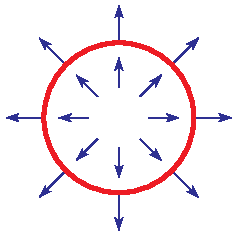
\includegraphics{sourceDiv.pdf}
\end{center}
\end{nfig}
This velocity field has fluid being created and pushed out through
the sphere. We have
\begin{align*}
\vnabla\cdot\vv(\vZero) = 3
\end{align*}
consistent with our interpretation \eqref{eq:divInterp}.
\end{eg}


\begin{eg}\label{eg:divInterpB}
Here is a sketch of the vector field $\vv(x,y,z) = -y\,\hi+x\,\hj$
and a sphere centered on the origin, like $S_\veps$. 
\begin{nfig}
\begin{center}
    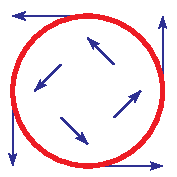
\includegraphics{vortexDiv.pdf}
\end{center}
\end{nfig}
This velocity field just has fluid going around in circles.
No fluid actually crosses the sphere. The divergence
\begin{align*}
\vnabla\cdot\vv(\vZero) = 0
\end{align*}
consistent with our interpretation \eqref{eq:divInterp}.
\end{eg}


\begin{eg}\label{eg:divInterpC}
Here is a sketch of the vector field $\vv(x,y,z) = \hi$
and a sphere centered on the origin, like $S_\veps$. 
\begin{nfig}
\begin{center}
    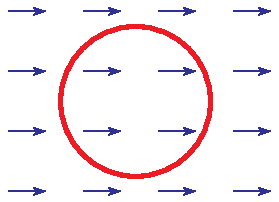
\includegraphics{transDiv.pdf}
\end{center}
\end{nfig}
This velocity field just has fluid moving uniformly to the right.
Fluid enters the sphere from the left and leaves through the right at 
precisely the same rate, so that the net rate at fluid crosses the 
sphere is zero. The divergence
\begin{align*}
\vnabla\cdot\vv(\vZero) = 0
\end{align*}
again consistent with our interpretation \eqref{eq:divInterp}.
\end{eg}



%\subsection{Optional --- Interpretation of the Curl}\label{sec:curlInterp}
\subsection{Interpretation of the Curl}\label{sec:curlInterp}

We'll now develop the interpretation of the curl, or
more precisely, of $\vnabla\times\vv(\vr_0)\cdot\hn$ for any unit vector $\hn$.
As we did in developing the interpretation of divergence, we'll
\begin{itemize}\itemsep1pt \parskip0pt \parsep0pt %\itemindent-15pt
\item[$\circ$]
first express $\vnabla\times\vv(\vr_0)\cdot\hn$ as a limit of integrals, and
\item[$\circ$] 
then we'll interpret the integrals.
\end{itemize}
To specify the integrals involved, let $C_\veps$ be the circle which 
\begin{itemize}\itemsep1pt \parskip0pt \parsep0pt %\itemindent-15pt
\item[$\circ$] is centered at $\vr_0$
\item[$\circ$] has radius $\veps$
\item[$\circ$] lies in the plane through $\vr_0$ perpendicular to $\hn$
\item[$\circ$] is oriented in the standard way with respect to $\hn$.
   Imagine standing on the circle with your feet on the plane through $\vr_0$ 
   perpendicular to $\hn$, with the vector from your feet to your head in the
   same direction as  $\hn$ and with your left arm point towards $\vr_0$.
   Then your are facing in the positive direction for $C_\veps$.
\end{itemize}
\begin{nfig}
\begin{center}
    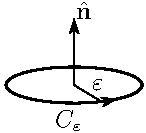
\includegraphics{prepaddle.pdf}
\end{center}
\end{nfig}
We shall show in Lemma \ref{lem:curlInterp}, below, that
\begin{equation*}%\label{eq:curlInterpB}
\vnabla\times v(\vr_0)\cdot \hn
=\lim_{\veps\rightarrow 0}\frac{1}{\pi\veps^2}
         \oint_{C_\veps} \vv(\vr)\cdot \dee{\vr}
\end{equation*}
Now let's work on interpreting the right hand side, and in particular
on interpreting the integral $\oint_{C_\veps} \vv(\vr)\cdot \dee{\vr}$,
which is called the circulation of $\vv$ around $C_\veps$.
Place a tiny paddlewheel in the fluid with its axle running along $\hn$
and its paddles along $C_\veps$, as in the figure below, except that
\vadjust{
\begin{nfig}
\begin{center}
    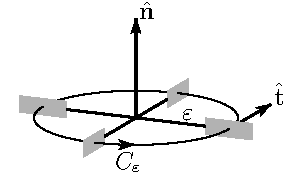
\includegraphics{paddle.pdf}
\end{center}
\end{nfig}
}
the paddlewheel is really expensive and has a lot more than just four
paddles. Pretend\footnote{Method acting might help you here.} that you are one of the paddles. 
\begin{itemize}
\item
If the paddlewheel is rotating at $\Om$ radians per unit time, then in one 
unit of time you sweep out an arc of a circle of radius $\veps$ that subtends 
an angle $\Om$. That arc has length $\Om\veps$. So you are moving at speed 
$\Om \veps$. 
\item
If you are at $\vr$, the component of the fluid velocity in your direction of motion, i.e. tangential to $C_\veps$, is $\vv(\vr)\cdot\diff{\vr}{s}$,
because $\hvt=\diff{\vr}{s}$, with $s$ denoting arc length along the circle, 
is a unit vector tangential to $C_\veps$. 
\item
All paddles have to move at the same speed. So the speed of the 
paddles, $\Om\veps$, should be the average value of $\vv(\vr)\cdot\diff{\vr}{s}$ around the circle.
\end{itemize}
Thus the rate of rotation, $\Om$, of the  paddlewheel should be
determined by
\begin{align*}
\Om \veps 
&= \frac{\oint_{C_\veps} \vv(\vr)\cdot\diff{\vr}{s}\dee{s}}
              {\oint_{C_\veps}\dee{s}} 
= \frac{\oint_{C_\veps} \vv(\vr)\cdot\dee{\vr}}
              {2\pi\veps} \\
\end{align*}
Consequently, $\vnabla\times v(\vr_0)\cdot \hn$ is the limit
as $\veps$ (the radius of the paddlewheel) tends to zero of
\begin{align*}
\frac{1}{\pi\veps^2}
         \oint_{C_\veps} \vv(\vr)\cdot \dee{\vr}
=2\Om
\end{align*}
That's our interpretation.
\begin{impeqn}\label{eq:curlInterp}
If a fluid has velocity field $\vv$ and you place an infinitesimal
paddlewheel at $\vr_0$ with its axle in direction $\vn$, then it rotates
at $\frac{1}{2}\vnabla\times \vv(\vr_0)\cdot \hn$ radians per unit time.
In particular, to maximize the rate of rotation, orient the paddlewheel so that
$\hn\parallel\vnabla\times \vv(\vr_0)$.
\end{impeqn}

There will be some examples at the end of this section.
First, we show

\begin{lemma}\label{lem:curlInterp}
\begin{equation*}
\vnabla\times \vv(\vr_0)\cdot \hn
=\lim_{\veps\rightarrow 0}\frac{1}{\pi\veps^2}
         \oint_{C_\veps} \vv(\vr)\cdot \dee{\vr}
\end{equation*}
\end{lemma}

\begin{proof}[Proof. (Optional)]\footnote{There is another, easier to understand, proof of this result given in \S\ref{sec:interpBis}. We cannot give that proof here because it uses Stokes' theorem, which we will get to
later in the chapter.}

Just as we did in the proof of Lemma \ref{lem:divInterp}, we can always
translate our coordinate system so that $\vr_0=(x_0,y_0,z_0) = (0,0,0)$. 
We can also rotate our coordinate system so that $\hn=\hk$. 
Because $\vr_0=(0,0,0)$ and $\hn=\hk$, so that $C_\veps$ lies in the 
$xy$-plane, we can parametrize $C_\veps$ by
\begin{equation*}
\vr(t) =\veps\cos t\,\hi +\veps\sin t\,\hj
\end{equation*}
Again as we did in the proof of Lemma \ref{lem:divInterp}, 
expand $\vv(x,y,z)$ in a Taylor expansion in powers of $x$, $y$, and $z$,
to first order, with second order error term.
\begin{align*}
\vv(x,y,z) = \vA + \vB\,x +\vC\,y +\vD\, z +\vR(x,y,z)
\end{align*}
where
\begin{align*}
\vA=\vv(0,0,0) \qquad
\vB=\frac{\partial \vv}{\partial x}(0,0,0) \qquad
\vC=\frac{\partial \vv}{\partial y}(0,0,0) \qquad
\vD=\frac{\partial \vv}{\partial z}(0,0,0) 
\end{align*}
and the error term $\vR(x,y,z)$ is bounded by a constant times
$x^2+y^2+z^2$. In particular there is a constant $K$ so that, on $C_\veps$,
\begin{equation*}
|\vR(x,y,z)|\le K\veps^2
\end{equation*}
So
\begin{align*}
\oint_{C_\veps} \vv(\vr)\cdot \dee{\vr}
&=\int_0^{2\pi} \big(\vA + \vB\,\veps\,\cos t +\vC\,\veps\,\sin t 
       +\vR(\vr(t))\big)
        \cdot \big(-\veps\sin t\,\hi +\veps\cos t\,\hj\big)\ \dee{t}
\end{align*}
Again, multiply out the dot product so that the integrand becomes
\begin{alignat*}{5}
& -\veps\vA\cdot\hi\,\sin t
&&+\ \veps\vA\cdot\hj\,\cos t \\ 
&-\veps^2\vB\cdot\hi\,\sin t\cos t
&&+\veps^2\vB\cdot\hj\,\cos^2t \\ 
&-\veps^2\vC\cdot\hi\,\sin^2 t 
&&+\ \veps^2\vC\cdot\hj\,\sin t\cos t \\ 
&+\vR(\vr(t))\cdot \big(-\veps\sin t\,\hi +\veps\cos t\,\hj\big)\hidewidth
\end{alignat*}
Again most of these terms integrate to zero, because
\begin{alignat*}{3}
\int_0^{2\pi}\sin t\ \dee{t}
   &=\hskip10pt\int_0^{2\pi}\cos t\ \dee{t}
   &&=0 \\
\int_0^{2\pi}\sin t\cos t\ \dee{t} 
&= \frac{1}{2}\int_0^{2\pi}\sin(2t)\ \dee{t}
&&=0
\end{alignat*}
and the $\sin^2t$ and $\cos^2 t$ terms are easily integrated using
(see Example \ref{eg:workIntegalB})
\begin{equation*}
\int_0^{2\pi}\sin^2 t\ \dee{t}=\int_0^{2\pi}\cos^2 t\ \dee{t}
=\frac{1}{2}\int_0^{2\pi}\big[\sin^2t+\cos^2 t\big]\ \dee{t}=\pi
\end{equation*}
So we are left with
\begin{align*}
\oint_{C_\veps} \vv(\vr)\cdot \dee{\vr} 
&= \pi\veps^2\vB\cdot\hj - \pi\veps^2\vC\cdot\hi
+\int_0^{2\pi} \vR(\vr(t))
        \cdot \big(-\veps\sin t\,\hi +\veps\cos t\,\hj\big)\ \dee{t}
\end{align*}
which implies that
\begin{align*}
&\lim_{\veps\rightarrow 0}\frac{1}{\pi\veps^2}
         \oint_{C_\veps} \vv(\vr)\cdot \dee{\vr} \\
&\hskip0.5in= \frac{\partial \vv_2}{\partial x}(0,0,0) 
  - \frac{\partial \vv_1}{\partial y}(0,0,0)
   +\lim_{\veps\rightarrow 0}\!
     \frac{1}{\pi\veps^2}
           \int_0^{2\pi}\!\!\!\! \vR(\vr(t))
        \cdot \big(-\veps\sin t\,\hi +\veps\cos t\,\hj\big)\,\dee{t} \\
&\hskip0.5in= \big(\vnabla\times\vv(0,0,0)\big)\cdot\hk
   +\lim_{\veps\rightarrow 0}
     \frac{1}{\pi\veps^2}
           \int_0^{2\pi} \vR(\vr(t))
        \cdot \big(-\veps\sin t\,\hi +\veps\cos t\,\hj\big)\ \dee{t}
\end{align*}
Finally, it suffices to recall that
$|\vR(x,y,z)|\le K\veps^2$, so that
\begin{align*}
\frac{1}{\pi\veps^2}\bigg|
            \int_0^{2\pi} \vR(\vr(t))
        \cdot \big(-\veps\sin t\,\hi +\veps\cos t\,\hj\big)\ \dee{t} \bigg|
&\le \frac{1}{\pi\veps}
            \int_0^{2\pi}|\vR(\vr(t))|\,\dee{t}  \\
&\le \frac{1}{\pi\veps}
           \int_0^{2\pi}K\veps^2\,\dee{t} 
= \frac{1}{\pi\veps} \ K\veps^2\,(2\pi) \\
&= 2K\veps
\end{align*}
converges to zero as $\veps\rightarrow 0$.

 \intremark{
To handle general $\hn$,
pick any three vectors $\hi',\ \hj',\ \hk'$ unit vectors such that
\begin{itemize}\itemsep1pt \parskip0pt \parsep0pt \itemindent 15pt
\item[$\circ$]  $\hk'=\hn$
\item[$\circ$] $\hi'\perp\hn$, $\hj'\perp\hn$
\item[$\circ$] $\hi'\times\hj'=\hk'$
\end{itemize}
and repeat the above argument with $\hi$, $\hj$, $\hk$ replaced by
$\hi'$, $\hj'$, $\hk'$.

Even if $\vr_0$ is not the origin we may parametrize $C_\veps$ by
\begin{equation*}
\vr(t)=\vr_0+\veps\cos t\ \hi'+\veps\sin t\ \hj'
\end{equation*}
So
\begin{align*}
&\oint_{C_\veps} \vv(\vr)\cdot \dee{\vr}
=\int_0^{2\pi} \vv\big(\vr_0+\veps\cos t\ \hi'+\veps\sin t\ \hj'\big)
\cdot\big(-\veps\sin t\ \hi'+\veps\cos t\ \hj'\big) \dee{t}\cr
&=\veps\int_0^{2\pi} \!\!\Big[
-\sin t\ \hi'\cdot\vv\big(\vr_0+\veps\cos t\ \hi'+\veps\sin t\ \hj'\big)
+\cos t\ \hj'\cdot\vv\big(\vr_0+\veps\cos t\ \hi'+\veps\sin t\ \hj'\big)\Big]\
\dee{t}
\end{align*}
Denote $f(\vr)=\hi'\cdot\vv(\vr)$.
Now Taylor expand 
$F(\veps)=f\big(\vr_0+\veps\cos t\ \hi'+\veps\sin t\ \hj'\big)$
about $\veps=0$.
\begin{align*}
F(\veps)&=F(0)+F'(0)\veps +O(\veps^2)\\
&=f\big(\vr_0\big)
+\veps\cos t\ \hi'\cdot\vnabla f\big(\vr_0\big)
+\veps\sin t\ \hj'\cdot\vnabla f\big(\vr_0\big) +O(\veps^2)\\
&=\hi'\cdot\vv\big(\vr_0\big)
+\veps\cos t\ \hi'\cdot\vnabla(\hi'\cdot\vv)\big(\vr_0\big)
+\veps\sin t\ \hj'\cdot\vnabla(\hi'\cdot\vv)\big(\vr_0\big) +O(\veps^2)
\end{align*}
Similarly, if $G(\veps)=\hj'\cdot\vv\big(\vr_0+\veps\cos t\ \hi'+\veps\sin t\ \hj'\big)$,
\begin{align*}
G(\veps)
&=\hj'\cdot\vv\big(\vr_0\big)
+\veps\cos t\ \hi'\cdot\vnabla(\hj'\cdot\vv)\big(\vr_0\big)
+\veps\sin t\ \hj'\cdot\vnabla(\hj'\cdot\vv)\big(\vr_0\big) +O(\veps^2)\cr
\end{align*}
Hence, the integrand
\begin{align*}
&-\sin t\ \hi'\cdot\vv\big(\vr_0+\veps\cos t\ \hi'+\veps\sin t\ \hj'\big) 
   \\&\hskip1in
+\cos t\ \hj'\cdot\vv\big(\vr_0+\veps\cos t\ \hi'+\veps\sin t\ \hj'\big)
\\
&\hskip0.5in= -\sin t\ \hi'\cdot\vv\big(\vr_0\big)
-\veps\sin t\cos t\ \hi'\cdot\vnabla(\hi'\cdot\vv)\big(\vr_0\big)
 -\veps\sin^2 t\ \hj'\cdot\vnabla(\hi'\cdot\vv)\big(\vr_0\big)
   \\&\hskip0.5in\phantom{=\ }
+\cos t\ \hj'\cdot\vv\big(\vr_0\big)
+\ \ \ \veps\cos^2 t\ \hi'\cdot\vnabla(\hj'\cdot\vv)\big(\vr_0\big)\ \ \ 
+\veps\sin t\cos t\ \hj'\cdot\vnabla(\hj'\cdot\vv)\big(\vr_0\big)+O(\veps^2)
\end{align*}
Since
\begin{equation*}
\int_0^{2\pi}\sin t\ \dee{t}=\int_0^{2\pi}\cos t\ \dee{t}
=\int_0^{2\pi}\sin t\cos t\ \dee{t}=0\qquad
\int_0^{2\pi}\sin^2 t\ \dee{t}=\int_0^{2\pi}\cos^2 t\ \dee{t}=\pi
\end{equation*}
we have
\begin{equation*}
\oint_{C_\veps} \vv(\vr)\cdot \dee{\vr}
=\pi\veps^2\Big[-\hj'\cdot\vnabla(\hi'\cdot\vv)\big(\vr_0\big)
    +\hi'\cdot\vnabla(\hj'\cdot\vv)\big(\vr_0\big)\Big]+O(\veps^3)
\end{equation*}
Substitute in 
\begin{equation*}
\hi'=-\hk'\times \hj'\qquad
\hj'=\hk'\times \hi'\qquad
\vnabla=\sum_{n=1}^3\hi_n\frac{\partial\hfill}{\partial x_n}
\end{equation*}
where we have renamed the standard basis for $\bbbr^3$ from $\hi,\hj,\hk$
to $\hi_1,\hi_2,\hi_3$ and the standard coordinates on $\bbbr^3$ from $x,y,z$
to $x_1,x_2,x_3$. Then
\begin{align*}
-\hj'\cdot\vnabla(\hi'\cdot\vv)\big(\vr_0\big)+\hi'\cdot\vnabla(\hj'\cdot\vv)\big(\vr_0\big)
&=\sum_{n=1}^3 -\hj'\cdot\hi_n\frac{\partial \hi'\cdot\vv}
{\partial x_n}\big(\vr_0\big)
+\sum_{n=1}^3\hi'\cdot\hi_n\frac{\partial \hj'\cdot\vv}{\partial x_n}\big(\vr_0\big)\cr
&\hskip-.5in=\sum_{n=1}^3 -(\hk'\times \hi')\cdot\hi_n\frac{\partial \hi'\cdot\vv}
{\partial x_n}\big(\vr_0\big)
+\sum_{n=1}^3-(\hk'\times \hj')\cdot\hi_n\frac{\partial \hj'\cdot\vv}{\partial x_n}\big(\vr_0\big)\cr
&\hskip-.5in=\sum_{n=1}^3 -\hk'\cdot( \hi'\times\hi_n)\frac{\partial \hi'\cdot\vv}
{\partial x_n}\big(\vr_0\big)
+\sum_{n=1}^3-\hk'\cdot( \hj'\times\hi_n)\frac{\partial \hj'\cdot\vv}{\partial x_n}\big(\vr_0\big)\cr
&\hskip-.5in=\sum_{n=1}^3 \hk'\cdot( \hi_n\times\hi')\frac{\partial \hi'\cdot\vv}
{\partial x_n}\big(\vr_0\big)
+\sum_{n=1}^3\hk'\cdot( \hi_n\times\hj')\frac{\partial \hj'\cdot\vv}{\partial x_n}\big(\vr_0\big)\cr
\end{align*}
Since $\hk'\perp \hi_n\times\hk'$,  $\hk'\cdot( \hi_n\times\hk')=0$
and
\begin{align*}
-\hj'\cdot\vnabla(\hi'\cdot\vv)\big(\vr_0\big)+\hi'\cdot\vnabla(\hj'\cdot\vv)
         \big(\vr_0\big)
&=\!\sum_{n=1}^3 \hk'\cdot \hi_n\!\times\!
\frac{\partial \hfill}{\partial x_n}
\big[\hi'(\hi'\cdot\vv)
+\hj'(\hj'\cdot\vv)
+\hk'(\hk'\cdot\vv)\big]\big(\vr_0\big)
\end{align*}
For any orthonormal basis, $\hi',\ \hj',\ \hk'$ and any vector $\vv$,
\begin{equation*}
\hi'(\hi'\cdot\vv)
+\hj'(\hj'\cdot\vv)
+\hk'(\hk'\cdot\vv)=\vv
\end{equation*}
so
\begin{equation*}
-\hj'\cdot\vnabla(\hi'\cdot\vv)\big(\vr_0\big)+\hi'\cdot\vnabla(\hj'\cdot\vv)\big(\vr_0\big)
=\sum_{n=1}^3 \hk'\cdot \hi_n\times
\frac{\partial \vv}{\partial x_n}(\vr_0)
=\hk'\cdot\vnabla\times \vv(\vr_0)
\end{equation*}
and
\begin{equation*}
\oint_{C_\veps} \vv(\vr)\cdot \dee{\vr} =\pi\veps^2\vnabla\times v(\vr_0)\cdot \hn
+O(\veps^3)
\end{equation*}
}

\end{proof}

Here are some examples. We will use the same vector fields as in Examples
\ref{eg:divInterpA}, \ref{eg:divInterpB} and \ref{eg:divInterpC}.
In all examples, we shall orient the paddlewheel so that $\hn=\hk$
and sketch the top view, so that the paddlewheel looks like
\begin{nfig}
\begin{center}
    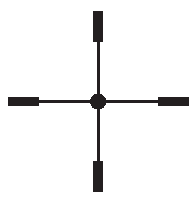
\includegraphics{paddlewheelTop.pdf}
\end{center}
\end{nfig}



\begin{eg}\label{eg:curlInterpA}
Here is a sketch of the vector field $\vv(x,y,z) = x\,\hi+y\,\hj+z\,\hk$
and a circle centered on the origin, like $C_\veps$. 
\begin{nfig}
\begin{center}
    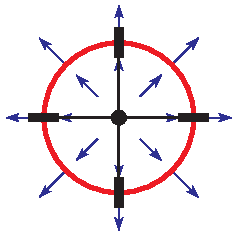
\includegraphics{sourceCurl.pdf}
\end{center}
\end{nfig}
This velocity field has fluid moving parallel to the paddles,
so the paddlewheel should not rotate at all. The computation
\begin{align*}
\vnabla\times\vv(\vZero) =
\det\left[\begin{matrix}
          \hi & \hj &\hk \\[0.05in]
          \frac{\partial\hfill}{\partial x} &
              \frac{\partial\hfill}{\partial y} &
              \frac{\partial\hfill}{\partial z}  \\
           x & y & z
          \end{matrix}
     \right] 
=\vZero
\implies \vnabla\times\vv(\vZero)\cdot\hk = 0
\end{align*}
is consistent with our interpretation \eqref{eq:curlInterp}.
\end{eg}


\begin{eg}\label{eg:curlInterpB}
Here is a sketch of the vector field $\vv(x,y,z) = -y\,\hi+x\,\hj$
and a circle centered on the origin, like $C_\veps$. 
\begin{nfig}
\begin{center}
    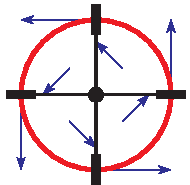
\includegraphics{vortexCurl.pdf}
\end{center}
\end{nfig}
This velocity field has fluid going around in circles, counterclockwise.
So the paddlewheel should rotate counterclockwise too. That is, it should
have positive angular velocity.
Our interpretation \eqref{eq:curlInterp} predicts an angular velocity of half
\begin{align*}
\vnabla\times\vv(\vZero)\cdot\hk =
\det\left[\begin{matrix}
          \hi & \hj &\hk \\[0.05in]
          \frac{\partial\hfill}{\partial x} &
              \frac{\partial\hfill}{\partial y} &
              \frac{\partial\hfill}{\partial z}  \\
           -y & x & 0
          \end{matrix}
     \right] \cdot\hk
=2\hk\cdot\hk
=2
\end{align*}
which is indeed positive\footnote{Even for small values of $2$.}.
\end{eg}


\begin{eg}\label{eg:curlInterpc}
Here is a sketch of the vector field $\vv(x,y,z) = \hi$
and a circle centered on the origin, like $C_\veps$. 
\begin{nfig}
\begin{center}
    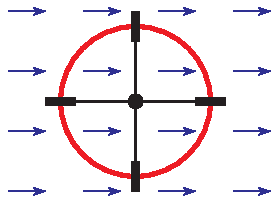
\includegraphics{transCurl.pdf}
\end{center}
\end{nfig}
The fluid pushing on the top paddle tries to make the paddlewheel rotate
clockwise. The fluid pushing on the bottom paddle tries to make the 
paddlewheel rotate counterclockwise, at the same rate.
So the paddlewheel should not rotate at all.
Our interpretation \eqref{eq:curlInterp} predicts an angular velocity of
\begin{align*}
\frac{1}{2}\cdot\vnabla\times\vv(\vZero)\cdot\hk 
=\frac{1}{2}
\det\left[\begin{matrix}
          \hi & \hj &\hk \\[0.05in]
          \frac{\partial\hfill}{\partial x} &
              \frac{\partial\hfill}{\partial y} &
              \frac{\partial\hfill}{\partial z}  \\
           1 & 0 & 0
          \end{matrix}
     \right] \cdot\hk
=\vZero\cdot\hk
=0
\end{align*}
as expected.
\end{eg}









\section{The Divergence Theorem}\label{sec:divergenceThm}
The rest of this chapter concerns three theorems: the divergence theorem,
Green's theorem and Stokes' theorem. Superficially, they look
quite different from each other. But, in fact, they are all \emph{very} 
closely related and all three are generalizations of the 
fundamental theorem of calculus
\begin{equation*}
\int_a^b \diff{f}{t}(t)\ \dee{t}
   = f(b) -f(a) 
\end{equation*}
The left hand side of the fundamental theorem of calculus is the 
integral of the derivative of a function.
The right hand side involves only values of the function on the boundary
of the domain of integration. The divergence theorem, Green's theorem
and Stokes' theorem also have this form, but the integrals are in more than 
one dimension. So the derivatives are multidimensional, like the curl
and divergence, and the integrands can involve vector fields.
\begin{itemize}
\item 
For the divergence theorem, the integral on the left hand side is over 
a (three dimensional) volume and the right hand side is an integral
over the boundary of the volume, which is a surface.
\item 
For Green's and Stokes' theorems, the integral on the left hand side is over 
a (two dimensional) surface and the right hand side is an integral
over the boundary of the surface, which is a curve.
\end{itemize}

The divergence theorem is going to relate a volume integral over a solid $V$
to a flux integral over the surface of $V$. First we need a couple of 
definitions concerning the allowed surfaces. In many applications solids,
for example cubes, have corners and edges where the normal vector is not defined. On the other hand, to be able to compute a flux integral over 
a surface, we certainly need that the set of points where  the normal vector
is not well-defined is small enough that the existence of the flux integral
is not jeopardized. This is the case for ``piecewise smooth'' surfaces,
which we now define.
\begin{defn}\label{def:pSmoothSurface}

\begin{enumerate}[(a)]
\item 
A surface is \emph{smooth} if it has a parametrization
$\vr(u,v)$ with continuous partial derivatives 
$\frac{\partial\vr}{\partial u}$ and $\frac{\partial\vr}{\partial v}$
and with $\frac{\partial\vr}{\partial u}\times\frac{\partial\vr}{\partial v}$
nonzero.

\item 
A surface is \emph{piecewise smooth} if it consists of a finite
number of smooth pieces that meet along sharp curves and at sharp corners.
\end{enumerate}
\end{defn}

\noindent Here are sketches of a smooth surface (a sausage) 
and a piecewise smooth surface (an ice-cream cone), followed by the
divergence theorem\footnote{It is also known as Gauss's theorem.
Johann Carl Friedrich Gauss (1777--1855) was a German mathematician.
Throughout the 1990's Gauss's portrait appeared on the German 
ten-mark banknote. In addition to Gauss's theorem, the Gaussian 
distribution (the bell curve), degaussing and the CGS unit for the 
magnetic field, and the crater Gauss on the Moon are named in his honour.}.
\begin{nfig}
\begin{center}
    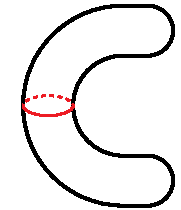
\includegraphics{divGenA.pdf}\qquad\quad
    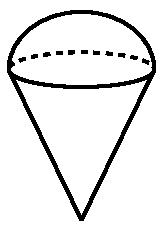
\includegraphics{pSmoothB.pdf}
\end{center}
\end{nfig}

\begin{theorem}[Divergence Theorem]\label{thm:divThm}
Let 
\begin{itemize}\itemsep1pt \parskip0pt \parsep0pt %\itemindent-15pt
\item
$V$ be a bounded solid with a piecewise smooth 
surface\footnote{We are going to consistently use the notation $\partial$(thing) to denote the boundary of (thing).} $\partial V$
\item
$\vF$ be a vector field that has continuous first partial derivatives 
at every point of $V$.
\end{itemize}
Then
\begin{align*}
\dblInt_{\partial V} \vF\cdot\hn\,\dee{S}
&=\tripInt_V\vnabla\cdot\vF\ \dee{V} 
\end{align*}
where $\hn$ is the outward unit normal of $\partial V$.
\end{theorem}

\intremark{
References:
\begin{itemize} 
\item[$\circ$]
Wilfred Kaplan, \emph{Advanced Calculus}
\item[$\circ$]
O. D. Kellogg, \emph{Foundations of Potential Theory}

\end{itemize}
} 
\noindent
Like the fundamental theorem of calculus, the divergence theorem expresses 
the integral of a derivative of a function (in this case a vector-valued
function) over a region in terms of the values of the function on the boundary of the region.

\begin{warning}\label{warn:divThm}
Note that in Theorem \ref{thm:divThm} we are assuming that
the vector field $\vF$ has continuous first partial derivatives 
at \emph{every} point of $V$.
If that is not the case, for example
because $\vF$ is not defined on all of $V$, then 
the conclusion of the divergence theorem can fail. An example is
$\vF = \frac{\vr}{|\vr|^3}$, $V=\Set{(x,y,z)}{x^2+y^2+z^2\le 1}$.
See Example~\ref{eg:divThmD}.
\end{warning}

\begin{proof}
We have to show that
\begin{align*}
\dblInt_{\partial V} \Big(
     \vF_1\,\hi + \vF_2\,\hj + \vF_3\,\hk\Big)
     \cdot\hn\,\dee{S}
&=\tripInt_V\Big(
     \frac{\,\partial \vF_1}{\partial x}
     +\frac{\partial \vF_2}{\partial y}
     +\frac{\partial \vF_3}{\partial z}\Big)
     \ \dee{V} 
\end{align*}
Note that the left hand side is a sum of three terms --- one involving $\vF_1$,
one involving $\vF_2$ and one involving $\vF_3$ ---
and the right hand side is a sum of three terms --- one involving $\vF_1$,
one involving $\vF_2$ and one involving $\vF_3$. We'll  just show that
the $\vF_3$ terms on the left hand side and right hand side are equal, i.e. 
that
\begin{align*}
\dblInt_{\partial V}  \vF_3\,\hk \cdot\hn\,\dee{S}
&=\tripInt_V
     \frac{\partial \vF_3}{\partial z}
     \ \dee{V} 
\end{align*}
Showing that the $\vF_1$ terms match and the $\vF_2$ terms match is done 
in the same way\footnote{Mutatis mutandis.}.

\medskip
\noindent \emph{Special Geometry}

We'll first assume that the solid has the special form
\begin{equation*}
V = \Set{(x,y,z)}{ B(x,y)\le z\le T(x,y),\ \ (x,y)\in R_{xy}}
\end{equation*}
where $R_{x,y}$ is some subset of the $xy$-plane. We can further assume
that, for each $(x,y)~\in~R_{xy}$, we have $B(x,y)\le  T(x,y)$.
After we're finished with this special case, we'll handle the general case.



\intremark{

\noindent Old version:

We'll first assume that the solid has the special form
\begin{equation*}
V = \Set{(x,y,z)}{ B(x,y)\le z\le T(x,y),\ \ (x,y)\in R_{xy}}
\end{equation*}
where $R_{x,y}$ is some subset of the $xy$-plane. 
For solids of this form, if you fix any $x=x_0$ and $y=y_0$,
then set of $z$-coordinates for which $(x_0,y_0,z)$ lies in the solid
are either 
\begin{itemize}\itemsep1pt \parskip0pt \parsep0pt %\itemindent-15pt
\item[$\circ$]
an interval, namely $\big[B(x_0,y_0), T(x_0,y_0)\big]$,
if $B(x_0,y_0)< T(x_0,y_0)$ or
\item[$\circ$]
a single point, namely $\big\{B(x_0,y_0)\big\}$,
if $B(x_0,y_0)= T(x_0,y_0)$, or
\item[$\circ$] the empty set if $B(x_0,y_0)> T(x_0,y_0)$
or if $(x_0,y_0)\notin R_{xy}$.
\end{itemize}
The interval case is illustrated by the leftmost line in the figure below;
the single point case is illustrated by the middle line; and the empty set
case is illustrated by the rightmost line.
\begin{nfig}
\begin{center}
    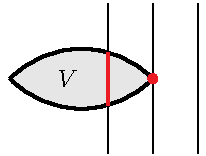
\includegraphics{divSpec.pdf}
\end{center}
\end{nfig}
\noindent
After we're finished with this special case, we'll handle the general case.
}

Let's work on $\dblInt_{\partial V}  \vF_3\,\hk \cdot\hn\,\dee{S}$
first.
As in the figure below, 
\vadjust{
\begin{nfig}
\begin{center}
    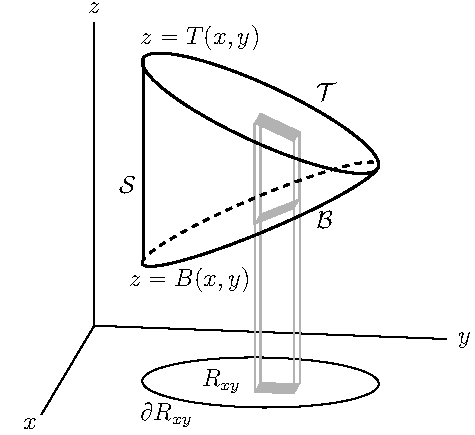
\includegraphics{divthm.pdf}
\end{center}
\end{nfig}
}
the surface $\partial V$ consists of three pieces --- the top, the bottom and 
the side. We'll consider each in turn.

\begin{itemize}\itemsep1pt \parskip0pt \parsep0pt %\itemindent-15pt
\item[$\circ$]
The top is $\cT=\Set{(x,y,z)}{ z= T(x,y),\ \ (x,y)\in R_{xy}}$.
By \eqref{eq:SUdSgraph}, on $\cT$
\begin{equation*}
\hn\, \dee{S}  = +\big[-T_x(x,y)\,\hi - T_y(x,y)\,\hj + \hk\big]\ 
          \dee{x}\dee{y}
\end{equation*}
As $\hn$ is to be the outward normal, it must point upwards on $\cT$.
That's why we have chosen, and emphasised, the ``$+$'' sign. So $\hk\cdot\hn\,\dee{S} = 
\dee{x}\dee{y}$ and
\begin{equation*}
\dblInt_{\cT}  \vF_3\,\hk \cdot\hn\,\dee{S}
=\dblInt_{R_{xy}}  \vF_3(x,y,T(x,y))\,\dee{x}\dee{y}
\end{equation*}

\item[$\circ$]
The bottom is 
$\cB=\Set{(x,y,z)}{ z= B(x,y),\ \ (x,y)\in R_{xy}}$.
By \eqref{eq:SUdSgraph}, on $\cB$
\begin{equation*}
\hn\, \dee{S}  = -\big[-B_x(x,y)\,\hi - B_y(x,y)\,\hj + \hk\big]\ 
          \dee{x}\dee{y}
\end{equation*}
As $\hn$ is to be the outward normal, it must point downwards on $\cB$.
That's why we have chosen the ``$-$'' sign. So $\hk\cdot\hn\,\dee{S} = 
-\dee{x}\dee{y}$ and
\begin{equation*}
\dblInt_{\cB}  \vF_3\,\hk \cdot\hn\,\dee{S}
=-\dblInt_{R_{xy}}  \vF_3(x,y,B(x,y))\,\dee{x}\dee{y}
\end{equation*}

\item[$\circ$]
The side is $\cS=\Set{(x,y,z)}{(x,y)\in\partial R_{xy},\ B(x,y)\le z\le T(x,y)}$. It runs vertically. Hence on  $\cS$ the normal vector to $\partial V$ 
is parallel to the $xy$-plane so that $\hk\cdot\hn=0$ and
\begin{equation*}
\dblInt_{\cS}  \vF_3\,\hk \cdot\hn\,\dee{S} = 0
\end{equation*}
\end{itemize}

So all together
\begin{align}
\dblInt_{\partial V}  \vF_3\,\hk \cdot\hn\,\dee{S}
&=\dblInt_{\cT}  \vF_3\,\hk \cdot\hn\,\dee{S}
 +\dblInt_{\cB}  \vF_3\,\hk \cdot\hn\,\dee{S}
 +\dblInt_{\cS}  \vF_3\,\hk \cdot\hn\,\dee{S} \notag\\
&=\dblInt_{R_{xy}}  \big[\vF_3(x,y,T(x,y))
   -\vF_3(x,y,B(x,y))\big]\,\dee{x}\dee{y}
   +0
\tag{$\partial V$}
\end{align}

Now let us examine
\begin{align}
\tripInt_V\frac{\partial \vF_3}{\partial z}\ \dee{V} 
&= \dblInt_{R_{xy}}\dee{x}\dee{y}\int_{B(x,y)}^{T(x,y)}\dee{z}\ 
            \frac{\partial \vF_3}{\partial z}(x,y,z) \notag\\
&=\dblInt_{R_{xy}}  \big[\vF_3(x,y,T(x,y))
   -\vF_3(x,y,B(x,y))\big]\,\dee{x}\dee{y}
\tag{$V$}
\end{align}
by the fundamental theorem of calculus.
That's exactly what we had to show. The integrals ($\partial V$)
and ($V$) are equal.


\medskip
\noindent \emph{General Geometry}

Now we'll drop the assumption on $V$ that we imposed in the ``Special 
Geometry'' section above. The key idea that makes the proof work 
is that we can cut up any\footnote{We are assuming that $V$ is
``reasonable''.} $V$ into pieces, each of which does obey the 
special assumption that we just considered. Consider, for example, 
the sausage shaped solid in the figure on the left below.
\begin{nfig}
\begin{center}
    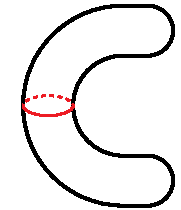
\includegraphics{divGenA.pdf}\qquad\qquad
    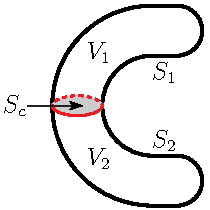
\includegraphics{divGen.pdf}
\end{center}
\end{nfig}
Call the sausage $V$.
Cut it into two halves by running a cleaver horizontally through its
centre. This splits the solid $V$ into two halves, $V_1$ and $V_2$
as in the figure on the right above. It also splits the boundary $\partial V$
of $V$ into two halves $S_1$ and $S_2$, also as in the figure on
the right above. Note that
\begin{itemize}\itemsep1pt \parskip0pt \parsep0pt %\itemindent-15pt
\item[$\circ$]
the boundary, $\partial V_1$, of $V_1$ is the union of $S_1$
and the shaded disk $S_c$ (the cut introduced by the cleaver). 
On the cut $S_c$, the outward pointing normal to $V_1$ is $-\hk$.
\item[$\circ$]
The boundary, $\partial V_2$, of $V_2$ is the union of $S_2$
and the shaded disk $S_c$. 
On the cut $S_c$, the outward pointing normal to $V_2$ is $+\hk$.
\end{itemize}
Now both $V_1$ and $V_2$ do satisfy the assumption of the ``Special Geometry''
section above. So
\begin{align*}
\tripInt_V\frac{\partial \vF_3}{\partial z}\ \dee{V} 
&= \tripInt_{V_1}\frac{\partial \vF_3}{\partial z}\ \dee{V} 
  +\tripInt_{V_2}\frac{\partial \vF_3}{\partial z}\ \dee{V} \\
&=\dblInt_{\partial V_1}  \vF_3\,\hk \cdot\hn\,\dee{S}
  +\dblInt_{\partial V_2}  \vF_3\,\hk \cdot\hn\,\dee{S} \\
&=\dblInt_{S_1}  \vF_3\,\hk \cdot\hn\,\dee{S}
  +\dblInt_{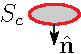
\includegraphics{SCdn.pdf}}  \vF_3\,\hk \cdot\hn\,\dee{S}
  +\dblInt_{S_2}  \vF_3\,\hk \cdot\hn\,\dee{S} 
  +\dblInt_{\raisebox{5pt}[23pt][10pt]{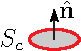
\includegraphics{SCup.pdf}}}  \vF_3\,\hk \cdot\hn\,\dee{S}
\end{align*}
The second and fourth integrals  are identical
except that $\hn=-\hk$ in the second integral and $\hn=+\hk$ in the
fourth integral. So they cancel exactly and
\begin{align*}
\tripInt_V\frac{\partial \vF_3}{\partial z}\ \dee{V} 
&=\dblInt_{S_1}  \vF_3\,\hk \cdot\hn\,\dee{S}
  +\dblInt_{S_2}  \vF_3\,\hk \cdot\hn\,\dee{S} 
=\dblInt_{\partial V}  \vF_3\,\hk \cdot\hn\,\dee{S}
\end{align*}
as desired.
\end{proof}

\begin{eg}\label{eg:divThmA}
\noindent\textit{Problem}:
Evaluate the flux integral $\dblInt_S \vF\cdot\hn\,\dee{S}$ where
$\hn $ is the outward normal to $S$, which is the surface of 
the hemispherical region
\begin{equation*}
V=\Set{(x,y,z)}{x^2+y^2+z^2\le a^2,\ z\ge 0}
\hskip0.5in\raisebox{-37pt}[30pt][20pt]
                         {\smash{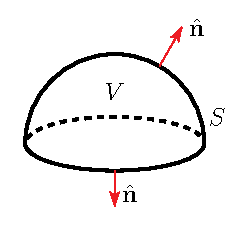
\includegraphics{hemisphere}}}
\end{equation*}
and
\begin{equation*}
\vF = xz^2\,\hi + (x^2y-z^3)\,\hj + \big(2xy + y^2 z +e^{\cos y}\big)\hk
\end{equation*}

\medskip
\noindent\textit{Solution}. The $e^{\cos y}$ in $\vF$ suggests that
a direct evaluation of the integral is difficult. So we'll use a 
little trickery to to evaluate it. Not surprisingly, 
considering that we have just proven the divergence theorem, the trick 
is to apply the divergence theorem\footnote{It's almost as though someone 
rigged the example with this in mind.}.
Since
\begin{align*}
\vnabla\cdot\vF &= \frac{\partial \vF_1}{\partial x}
                 +\frac{\partial \vF_2}{\partial y}
                 +\frac{\partial \vF_3}{\partial z}
=\frac{\partial\hfill}{\partial x}\big(xz^2\big)
+\frac{\partial\hfill}{\partial y}\big(x^2y-z^3\big)
+\frac{\partial\hfill}{\partial z}\big(2xy + y^2 z +e^{\cos y}\big) \\
&= z^2 + x^2 +y^2
\end{align*}
The divergence theorem tell us that
\begin{align*}
\dblInt_S \vF\cdot\hn\,\dee{S}
&=\tripInt_V\big(x^2+y^2+z^2\big)\ \dee{V}
\end{align*}
Spherical coordinates are perfect for this integral. (See 
Appendix \ref{ap:spherCoord}, if you need to refresh your memory.)
\begin{align*}
\tripInt_V\big(x^2+y^2+z^2\big)\ \dee{V}
&=\int_0^{2\pi}\dee{\theta}\int_0^{\nicefrac{\pi}{2}}\dee{\varphi}
   \int_0^a \dee{\rho}\,\rho^2\sin\varphi\ \rho^2 \\
&=\bigg[\int_0^{2\pi}\dee{\theta}\bigg]
\bigg[\int_0^{\nicefrac{\pi}{2}}\sin\varphi\,\dee{\varphi}\bigg]
\bigg[\int_0^{a}\rho^4\,\dee{\rho}\bigg] \\
&=\big[2\pi\big]\Big[-\cos\varphi\Big]_0^{\nicefrac{\pi}{2}}
   \left[\frac{\rho^5}{5}\right]_0^a \\
&=\frac{2\pi a^5}{5}
\end{align*}


\end{eg}

\begin{eg}\label{eg:divThmB}
\noindent\textit{Problem}:
Evaluate the flux integral $\dblInt_S \vF\cdot\hn\,\dee{S}$ where
$\hn $ is the outward normal to $S$, which is the part of the surface
$z^2=x^2+y^2$ with $1\le z\le 2$, and where
\begin{equation*}
\vF = 3x\,\hi + (5y+e^{\cos x})\,\hj + z\,\hk
\end{equation*}

\medskip
\noindent\textit{Solution}. 
Again the $e^{\cos x}$ in $\vF$ suggests that a direct evaluation 
is difficult\footnote{In fact, it is possible to evaluate this integral directly, if one recognizes that the ugly part of the integrand 
is odd under $y\rightarrow-y$ and integrates to exactly zero. } 
and again we'll apply the divergence theorem. But this time
$S$ is not the boundary of a solid $V$. It is the portion of the cone outlined
in red in the figure on the left below and does not have a top or 
bottom ``cap''.
\vadjust{
\begin{efig}
\begin{center}
    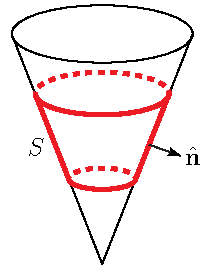
\includegraphics{coneP.pdf}\qquad\qquad
    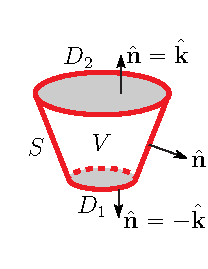
\includegraphics{coneB.pdf}
\end{center}
\end{efig}
}
Fortunately, there is a solid $V$ whose boundary, while not being equal to  
$S$, at least contains $S$. It is (unsurprisingly)
\begin{equation*}
V = \Set{(x,y,z)}{x^2+y^2\le z^2,\ \ 1\le z\le 2}
\end{equation*}
and is sketched in the figure on the right above.
The boundary, $\partial V$, is the union of $S$ and the two disks
\begin{align*}
D_1 &= \Set{(x,y,z)}{x^2+y^2\le z^2,\ \ z=1} \\
D_2 &= \Set{(x,y,z)}{x^2+y^2\le z^2,\ \ z=2} 
\end{align*}
So the divergence theorem gives
\begin{align*}
\tripInt_V\vnabla\cdot\vF\ \dee{V} = \dblInt_{\partial V} \vF\cdot\hn\,\dee{S}
= \dblInt_S \vF\cdot\hn\,\dee{S}
 +\dblInt_{D_1} \vF\cdot\hn\,\dee{S}
 +\dblInt_{D_2} \vF\cdot\hn\,\dee{S}
\end{align*}
which implies
\begin{align*}
\dblInt_S \vF\cdot\hn\,\dee{S}
&= \tripInt_V\vnabla\cdot\vF\ \dee{V} 
  -\dblInt_{D_1} \vF\cdot\hn\,\dee{S}
 -\dblInt_{D_2} \vF\cdot\hn\,\dee{S}
\end{align*}
The point of this exercise is that the left hand side, which is not easy
to evaluate directly, is the integral we want, while the three
integrals on the right hand side are all easy to evaluate. We do so now.
The outward normal to (the horizontal disk) $D_2$ is $+\hk$. So
\begin{align*}
\dblInt_{D_2} \vF\cdot\hn\,\dee{S}
&=\dblInt_{D_2} \vF\cdot\hk\,\dee{S}
=\dblInt_{D_2} z\,\dee{S}
\end{align*} 
As $z=2$ on $D_2$, and $D_2$ is a disk of radius $2$,
\begin{equation*}
\dblInt_{D_1} \vF\cdot\hn\,\dee{S}
=2\text{Area}(D_2)
=2\pi 2^2 = 8\pi
\end{equation*}
Similarly, the outward normal to (the horizontal disk) $D_1$ is $-\hk$. So
\begin{align*}
\dblInt_{D_1} \vF\cdot\hn\,\dee{S}
&=-\dblInt_{D_1} \vF\cdot\hk\,\dee{S}
=-\dblInt_{D_1} z\,\dee{S}
\end{align*} 
As $z=1$ on $D_1$, and $D_1$ is a disk of radius $1$,
\begin{equation*}
\dblInt_{D_1} \vF\cdot\hn\,\dee{S}
=\text{Area}(D_1)
=-\pi 1^2 = -\pi
\end{equation*}
Finally, as $\vnabla\cdot\vF = 3+5+1 = 9$
\begin{align*}
\tripInt_V\vnabla\cdot\vF\ \dee{V}
=9\,\text{Vol}(V)
\end{align*}
The volume of $V$ can be easily computed using the first year 
technique\footnote{You can review in \S1.6 of the CLP-2 text.}
of slicing $V$ into thin horizontal pancakes like that sketched in the 
figure below.
\begin{nfig}
\begin{center}
    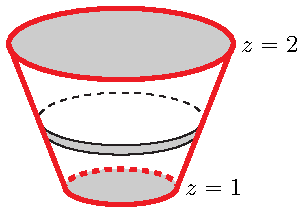
\includegraphics{coneC.pdf}
\end{center}
\end{nfig}
The pancake at height $z$ has 
\begin{itemize}\itemsep1pt \parskip0pt \parsep0pt %\itemindent-15pt
\item[$\circ$] 
thickness $\dee{z}$,
\item[$\circ$] 
a circular cross-section of radius $z$ (remember that the outer
boundary of $V$ has equation $x^2+y^2=z^2$), and hence has
\item[$\circ$] 
cross-sectional area $\pi z^2$ and
\item[$\circ$] 
volume $\pi z^2\,\dee{z}$.
\end{itemize}
So
\begin{align*}
\tripInt_V\vnabla\cdot\vF\ \dee{V}
=9\,\text{Vol}(V)
=9\int_1^2 \pi z^2\,\dee{z}
=9\left[\frac{\pi z^3}{3}\right]_1^2
=9\times \pi\frac{7}{3}
=21\pi
\end{align*}
and, all together
\begin{align*}
\dblInt_S \vF\cdot\hn\,\dee{S}
&= \tripInt_V\vnabla\cdot\vF\ \dee{V} 
  -\dblInt_{D_1} \vF\cdot\hn\,\dee{S}
 -\dblInt_{D_2} \vF\cdot\hn\,\dee{S}
= 21\pi - (-\pi) -8\pi
=14\pi
\end{align*}


\intremark{
To integrate the given integral directly use
\begin{equation*}
\hn\,\dee{S} = \frac{\vnabla(z^2-x^2-y^2)}{\hk\cdot\vnabla(z^2-x^2-y^2)}
                       \dee{x}\dee{y}
             =\frac{-x\,\hi - y\,\hj +z\,\hk}{z}\dee{x}\dee{y}
\end{equation*}
so that
\begin{equation*}
\vF\cdot\hn\,\dee{S} 
=\frac{-3x^2-5y^2-ye^{\cos x}+z^2}{z}\dee{x}\dee{y}
\end{equation*}
with $z = \sqrt{x^2+y^2}$ and with domain of integration $1\le x^2+y^2\le 4$.
The term $-\frac{y}{z}e^{\cos x}$ will integrate to $0$ because it is
odd under $y\rightarrow-y$. The rest can be integrated using polar coordinates.
}

\end{eg}

\begin{eg}\label{eg:divThmC}
\noindent\textit{Problem}:
Evaluate the flux integral $\dblInt_S \vF\cdot\hn\,\dee{S}$ where
$\hn $ is the upward normal to $S$, which is the part of 
$z={\big(x^2+y^2\big)}^2$ with $0\le z\le 1$, and
\begin{equation*}
\vF = \big(x+e^{y^2}\big)\,\hi + (y+\cos z)\,\hj + \hk
\end{equation*}

\medskip
\noindent\textit{Solution}.
This integral can be evaluated in much the same way as we evaluated 
the integral of Example~\ref{eg:divThmB}. We first define a solid $V$ 
whose boundary $\partial V$ contains $S$. A good, and hopefully obvious, 
choice is
\begin{align*}
V = \Set{(x,y,z)}{{\big(x^2+y^2\big)}^2\le z,\ \ 0\le z\le 1 }
\end{align*}
The boundary of $V$ is the union of $S$, with outward pointing normal $-\vn$
(recall that the problem specifies that the symbol $\hn$ refers to
the upward pointing normal)  and the disk
\begin{equation*}
D = \Set{(x,y,z)}{z= 1,\ \  {\big(x^2+y^2\big)}^2\le 1}
\end{equation*}
with outward pointing normal $\hk$.
\begin{nfig}
\begin{center}
    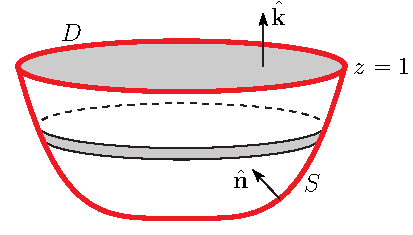
\includegraphics{bowl.pdf}
\end{center}
\end{nfig}
So the divergence theorem gives
\begin{align*}
\tripInt_V\vnabla\cdot\vF\ \dee{V} 
= -\dblInt_S \vF\cdot\hn\,\dee{S}
 +\dblInt_{D} \vF\cdot\hk\,\dee{S}
\end{align*}
which implies
\begin{align*}
\dblInt_S \vF\cdot\hn\,\dee{S}
&= -\tripInt_V\vnabla\cdot\vF\ \dee{V} 
  +\dblInt_{D} \vF\cdot\hk\,\dee{S} \\
&= -\tripInt_V 2\ \dee{V} 
  +\dblInt_{D} \dee{S} 
\end{align*}
$D$ is a circular disk of radius $1$, and so has area $\pi$. To evaluate the
volume integral we slice $V$ into horizontal pancakes with the pancake at height $z$ having a circular cross-section of radius $z^{\nicefrac{1}{4}}$. 
(Recall that the boundary of $V$ has ${\big(x^2+y^2\big)}^2 = z$.) So 
\begin{align*}
\dblInt_S \vF\cdot\hn\,\dee{S}
&= -2\int_0^1\pi \sqrt{z}\ \dee{z} 
  +\pi 
=-2\pi\times\frac{2}{3} +\pi
=-\frac{\pi}{3}
\end{align*}
Again, you can see that the actual integration is quite easy. All of the work 
(or at least all of the thinking) happens in the setup.
\end{eg} 

\begin{eg}\label{eg:divThmD}
In Warning \ref{warn:divThm} we emphasised that the conclusion of the
divergence Theorem \ref{thm:divThm} can fail if
the vector field $\vF$ is not defined at even a single
point of $V$. Here is an example. Set
\begin{equation*}
\vF = \frac{\vr}{|\vr|^3}
\qquad\text{where $\vr=x\,\hi+y\,\hj +z\,\hk$}
\end{equation*}
and $V=\Set{(x,y,z)}{x^2+y^2+z^2\le 1}$.
Then, if $(x,y,z)\ne\vZero$,
\begin{align*}
\vnabla\cdot\vF(x,y,z)
&=\frac{\partial\hfill}{\partial x}\frac{x}{{\big[x^2+y^2+z^2\big]}^{3/2}}
+\frac{\partial\hfill}{\partial y}\frac{y}{{\big[x^2+y^2+z^2\big]}^{3/2}}
+\frac{\partial\hfill}{\partial z}\frac{z}{{\big[x^2+y^2+z^2\big]}^{3/2}}
\\
&=\frac{\big[x^2+y^2+z^2\big]-x\frac{3}{2}(2x)}{{\big[x^2+y^2+z^2\big]}^{5/2}}
+\frac{\big[x^2+y^2+z^2\big]-y\frac{3}{2}(2y)}{{\big[x^2+y^2+z^2\big]}^{5/2}}
+\frac{\big[x^2+y^2+z^2\big]-z\frac{3}{2}(2z)}{{\big[x^2+y^2+z^2\big]}^{5/2}}
\\
&=0
\end{align*}
On the other hand, the boundary of $V$ is the unit sphere
$\partial V = \Set{(x,y,z)}{x^2+y^2+z^2 = 1}$. The outward unit 
normal to $\partial V$
is $\hn = \frac{\vr}{|\vr|}$ so that
\begin{align*}
\int_{\partial V}\vF\cdot\hn\ \dee{S}
&=\int_{|\vr|=1}  \frac{\vr}{|\vr|^3}\cdot \frac{\vr}{|\vr|}\ \dee{S} 
=\int_{|\vr|=1}  \frac{1}{|\vr|^2}\ \dee{S}
=\int_{|\vr|=1}\dee{S} \\
&=4\pi\ne 0
\end{align*}


\end{eg}



\subsection{Optional --- An Application of the Divergence Theorem --- the Heat Equation}  \label{sec:heatEqn}

\subsubsection{Derivation of the Heat Equation}

Let $T(x,y,z,t)$ be the temperature at time $t$ at the point $(x,y,z)$
in some object $\cB$. The heat equation\footnote{The heat equation was 
formulated by the French mathematician and physicist Jean-Baptiste 
Joseph Fourier in 1807. He lived from 1768 to 1830, a period which 
included both the French revolution and the reign of Napoleon. Indeed 
Fourier served on his local Revolutionary Committee, was imprisoned 
briefly during the Terror, and was Napoleon Bonaparte's scientific 
advisor on his Egyptian expedition of 1798. Fourier series and 
the Fourier transform are named after him. Fourier is also credited 
with discovering the greenhouse effect.}  
is the partial differential equation 
that describes the flow of heat energy and consequently the behaviour of
$T$. We now use the divergence theorem to derive the heat 
equation
from two physical ``laws'', that we assume are valid:
\begin{itemize}\itemsep1pt \parskip0pt \parsep0pt %\itemindent-15pt
\item[$\circ$] 
The amount of heat energy required to raise the temperature
of an object by $\De T$ degrees is $CM\,\De T$ where, $M$ is the mass 
of the object and $C$ is a positive physical constant determined by the 
material contained in the object. It is called the specific heat, or specific heat capacity\footnote{
Heat is now understood to arise from the internal energy of the object.
In an earlier theory, heat was viewed as measuring an invisible fluid, 
called the caloric. The amount of caloric that an object could hold 
was called its ``heat capacity'' by the Scottish physician and chemist 
Joseph Black (1728--1799).}, of the object.
\item[$\circ$]
Think of heat energy as a moving fluid. We will rig its velocity field so
that heat flows in the direction opposite to the temperature gradient.
Precisely, we choose its velocity field to be $-\ka\vnabla T(x,y,z,t)$. 
Here $\ka$ is another positive physical constant called the thermal 
conductivity of the object. So the rate at which heat is conducted
across an element of surface area $\dee{S}$ at $(x,y,z)$ in the direction of 
its unit normal $\hn$ is given by $-\ka\hn\cdot\vnabla T(x,y,z,t)\,\dee{S}$ at 
time $t$. (See Lemma \ref{lem:fluxInterp}.) For example, in the figure
\begin{nfig}
\begin{center}
    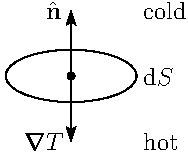
\includegraphics{heat1.pdf}
\end{center}
\end{nfig}
the temperature gradient, which points in the direction of 
increasing temperature, is opposite $\hn$. Consequently the flow rate 
$-\ka\hn\cdot\vnabla T(x,y,z,t)\,\dee{S}$ is positive, indicating flow in the 
direction of $\hn$. This is just what you would expect --- heat flows from
hot regions to cold regions. Also the rate of flow increases as the 
magnitude of the temperature gradient increases. This also makes sense
(and is reminiscent of Newton's law of cooling).
\end{itemize}
\noindent
Let $V\subset\cB$ be \emph{any} three dimensional region in the object and denote 
by $\partial V$ the surface of $V$ and by $\hn$ the outward normal to 
$\partial V$. The amount of heat that \emph{enters} $V$ across an infinitesimal
piece $\dee{S}$ of $\partial V$ in an infinitesimal time interval $\dee{t}$ is
$-\big(-\ka\hn\cdot\vnabla T(x,y,z,t)\,\dee{S}\big)\,\dee{t}$.
The amount of heat that enters $V$ across all of $\partial V$ in the
time interval $\dee{t}$ is given by the integral
\begin{equation*}
\dblInt_{\partial V} \ka\hn\cdot\vnabla T(x,y,z,t)\,\dee{S}\,\dee{t}
\hskip0.5in\raisebox{-32pt}[68pt][30pt]
                         {\smash{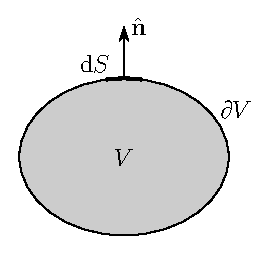
\includegraphics{heat2}}}
\end{equation*}
In this same time interval, the temperature at a point  $(x,y,z)$ in $V$
changes by $\frac{\partial T}{\partial t}(x,y,z,t)\,\dee{t}$. If the density of 
the object at $(x,y,z)$ is $\rho(x,y,z)$, the amount of heat energy  
required to increase the temperature of an infinitesimal volume $\dee{V}$ of 
the object centred at $(x,y,z)$ by  
$\frac{\partial T}{\partial t}(x,y,z,t)\,\dee{t}$
is $C(\rho\dee{V})\,\frac{\partial T}{\partial t}(x,y,z,t)\,\dee{t}$.
The amount of heat energy required
to increase the temperature by $\frac{\partial T}{\partial t}(x,y,z,t)\,\dee{t}$
at all points $(x,y,z)$ in $V$ is then
\begin{equation*}
\tripInt_V C\rho\frac{\partial T}{\partial t}(x,y,z,t)\,\dee{V}\,\dee{t}
\end{equation*}
Assuming that the object is not generating or destroying\footnote{The caloric theory of heat was itself destroyed by the cannon boring experiment of 1798.
In this experiment the American/British physicist Benjamin Thompson 
(1753--1814) boiled water just using the heat generated by friction 
during the boring of a cannon.} heat itself, this
must be same as the amount of heat that entered $V$ in the time interval
$\dee{t}$. That is
\begin{equation*}
\dblInt_{\partial V} \ka\hn\cdot\vnabla T\,\dee{S}\,\dee{t}
=\tripInt_V C\rho\frac{\partial T}{\partial t}\,\dee{V}\,\dee{t}
\end{equation*}
Now we cancel the common factor of $\dee{t}$. We can then rewrite the
left hand side as an integral over $V$ by applying the divergence theorem
giving
\begin{equation*}
\tripInt_{V} \ka\vnabla\cdot\vnabla T\,\dee{V}
=\tripInt_V C\rho\frac{\partial T}{\partial t}\,\dee{V}
\end{equation*}
As both integrals are over the same volume $V$, we have
\begin{equation}
\tripInt_{V} \ka\vnabla\cdot\vnabla T\,\dee{V}
-\tripInt_V C\rho\frac{\partial T}{\partial t}\,\dee{V}
=0
\implies 
\tripInt_{V} \left[\ka\vnabla^2 T
          -C\rho\frac{\partial T}{\partial t}\right]\,\dee{V}=0
\tag{H}\end{equation}
where $\vnabla^2=\vnabla\cdot\vnabla=\frac{\partial^2\hfill}{\partial x^2}+
\frac{\partial^2\hfill}{\partial y^2}+\frac{\partial^2\hfill}{\partial z^2}$
is the Laplacian.
This must be true for all volumes $V$ in the object and for all times $t$. We
claim that this forces 
\begin{equation*}
\ka\vnabla^2 T(x,y,z,t)-C\rho\frac{\partial T}{\partial t}(x,y,z,t)=0
\end{equation*}
for all $(x,y,z)$ in the object and all $t$.

Suppose that to the contrary there was a point $(x_0,y_0,z_0)$ in the object
and a time $t_0$ with, for example,
$\ka\vnabla^2 T(x_0,y_0,z_0,t_0)
   -C\rho\frac{\partial T}{\partial t}(x_0,y_0,z_0,t_0)>0$. 
By continuity, which we are assuming, $\ka\vnabla^2 T(x,y,z,t_0)
   -C\rho\frac{\partial T}{\partial t}(x,y,z,t_0)$
must remain close to $\ka\vnabla^2 T(x_0,y_0,z_0,t_0)
   -C\rho\frac{\partial T}{\partial t}(x_0,y_0,z_0,t_0)$ when $(x,y,z)$ 
is close to $(x_0,y_0,z_0)$.
So we would have 
\begin{equation*}
\ka\vnabla^2 T(x,y,z,t_0)
-C\rho\frac{\partial T}{\partial t}(x,y,z,t_0)>0
\end{equation*}
for all $(x,y,z)$ in some small ball $B$ centered on $(x_0,y_0,z_0)$. 
Then, necessarily,
\begin{equation*}
\tripInt_{B} \Big[\ka\vnabla\cdot\vnabla T(x,y,z,t_0)
      -C\rho\frac{\partial T}{\partial t}(x,y,z,t_0)\Big]\,\dee{V}>0
\end{equation*}
which violates (H) for $V=B$.  This completes our derivation of the 
heat equation, which is
\begin{impeqn}\label{eqn:heat}
\begin{equation*}
\frac{\partial T}{\partial t}(x,y,z,t)
=\alpha \vnabla^2 T(x,y,z,t)
\end{equation*}
where $\alpha=\frac{\ka}{C\rho}$ is called the thermal diffusivity.
\end{impeqn}


\subsubsection{An Application of the Heat Equation}
As an application, we look at the temperature a short distance 
below the surface of the Earth. For simplicity, we make the Earth 
flat\footnote{Insert sarcastic footnote here.}
and we assume that the temperature, $T$, depends only on time, $t$, and 
the vertical coordinate, $z$. Then the heat equation simplifies to
\begin{equation}
\frac{\partial T}{\partial t}(z,t)
=\alpha \frac{\partial^2 T}{\partial z^2}(z,t)
\tag{HE}\end{equation}
We choose a coordinate system having the
surface of the Earth at $z=0$ and having $z$ increase downward.
We also assume that the temperature $T(0,t)$ at the surface of the Earth
is primarily determined by solar heating and is given by
\begin{equation}
T(0,t)=T_0+T_A\cos(\sigma t)+T_D\cos(\delta t)
\tag{BC}\end{equation}
Here $T_0$ is the long term
average of the temperature at the surface of the Earth, 
$T_A\cos(\sigma t)$ gives seasonal temperature variations and 
$T_D\cos(\delta t)$ gives daily temperature variations.% 
\vadjust{
\begin{wfig}
\begin{center}
    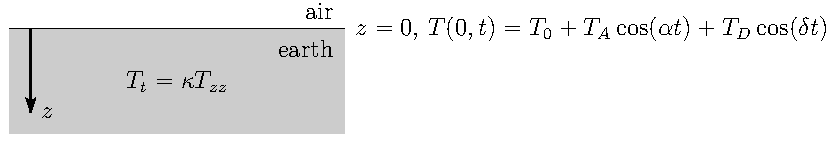
\includegraphics{heat3.pdf}
\end{center}
\end{wfig}
}
%We measure time in seconds so that 
%$\delta =\frac{2\pi}{1\ {\rm day}}=\frac{2\pi}{86,400 {\rm sec}}$ and 
%$\sigma =\frac{2\pi}{1\ {\rm year}}=\frac{2\pi}{3.15\times 10^7 {\rm sec}}$.
We measure time in days so that 
$\delta =2\pi$ and 
$\sigma =\frac{2\pi}{1\ {\rm year}}=\frac{2\pi}{365{\rm days}}$.
Then $T_A\cos(\sigma t)$ has period one year and 
$T_D\cos(\delta t)$ has period one day.
The solution to the initial value problem (HE)+(BC) can be found by separation
of variables, a standard topic in courses on partial differential equations.
The solution is
\begin{equation}
T(z,t)=T_0
+T_Ae^{-\sqrt{\sigma \over 2\alpha}\ z}
     \cos\Big(\sigma t-\sqrt{\frac{\sigma }{2\alpha}}\ z\Big)
+T_De^{-\sqrt{\delta \over 2\alpha}\ z}
 \cos\Big(\delta t-\sqrt{\frac{\delta }{2\alpha}}\ z\Big)
\tag{SLN}\end{equation}
Whether or not you can find this solution, 
you can, and should, check that (SLN) satisfies both (HE) and (BC). 

Now let's see what we can learn from the solution (SLN).
For any fixed $z$, the time average of $T(z,t)$ is $T_0$ (just because the average
value if cosine is zero), the same as the average temperature
at the surface $z=0$. That is, under the hypotheses that we have made,
the long term average temperature at any depth $z$ is is the same as 
the long term average temperature at the surface.

The term 
$T_Ae^{-\sqrt{\sigma \over 2\alpha}\ z}
           \cos\Big(\sigma t-\sqrt{\frac{\sigma }{2\alpha}}\   z\Big)$
\begin{itemize}\itemsep1pt \parskip5pt \parsep0pt %\itemindent-15pt
\item[$\circ$] 
oscillates in time with a period of one year, just like $T_A\cos(\sigma t)$
\item[$\circ$]
has an amplitude $T_Ae^{-\sqrt{\sigma \over 2\alpha}\ z}$ which
is $T_A$ at the surface and decreases exponentially as $z$ increases. 
Increasing the depth $z$ by a distance $\sqrt{\nicefrac{2\alpha}{\sigma}}$ 
causes the amplitude of the oscillation to decrease by a factor 
of $\nicefrac{1}{e}$. Both of these first two bullet points are probably
very consistent with your intuition. But this term also has a third property
that you may find less obvious. It has 
\item[$\circ$]
has a time lag of $\frac{z}{\sqrt{2\alpha\sigma}}$ with respect to 
$T_A\cos(\sigma t)$.
The surface term $T_A\cos(\sigma t)$ takes its maximum value when
$t=0,\ \nicefrac{2\pi}{\sigma},\ \nicefrac{4\pi}{\sigma},\ \cdots$. 
At depth $z$, the corresponding term $T_Ae^{-\sqrt{\sigma \over 2\alpha}\ z}
         \cos\Big(\sigma t-\sqrt{\nicefrac{\sigma }{2\alpha}}\ z\Big)$
takes its maximum value when $\ \sigma t-\sqrt{\nicefrac{\sigma }{2\alpha}}\ z
        =0,\ 2\pi, 4\pi,\ \cdots$ so that
$t=\nicefrac{z}{\sqrt{2\alpha\sigma}},\ \nicefrac{2\pi}{\sigma}+\nicefrac{z}{\sqrt{2\alpha\sigma}},
\ \nicefrac{4\pi}{\sigma}+\nicefrac{z}{\sqrt{2\alpha\sigma}},\ \cdots$.
\end{itemize}
Similarly, the term 
$T_De^{-\sqrt{\delta \over 2\alpha}\ z}
          \cos\Big(\delta t-\sqrt{\frac{\delta }{2\alpha}}\ z\Big)$
\begin{itemize}\itemsep1pt \parskip5pt \parsep0pt %\itemindent-15pt
\item[$\circ$] 
oscillates in time with a period of one day, just like $T_D\cos(\delta t)$
\item[$\circ$]
has an amplitude which is $T_D$ at the surface and decreases by a 
factor of $\nicefrac{1}{e}$ for each increase of 
$\sqrt{\nicefrac{2\alpha}{\delta}}$  in depth.
\item[$\circ$]
has a time lag of $\frac{z}{\sqrt{2\alpha\delta}}$ with respect to 
$T_D\cos(\delta t)$.
\end{itemize}
For water $\alpha$ is approximately $0.012$ m$^2$/day. This $\alpha$ gives 
\begin{equation*}
\sqrt{\frac{2\alpha}{\sigma}}\approx  1.2\,{\rm m}\qquad
\sqrt{\frac{2\alpha}{\delta}}\approx    0.062\,{\rm m} \qquad
\frac{z}{\sqrt{2\alpha\sigma}}\approx 49\, z\,{\rm days} \qquad
\frac{z}{\sqrt{2\alpha\delta}}\approx 2.6\, z\,{\rm days}
\end{equation*}
for $z$ measured in centimeters. So at a depth of a couple of meters,
the temperature is pretty constant in time. What variation there is
lags the surface variations by several months. 


\intremark{

\noindent
Thermal diffusivity table


\noindent
\renewcommand{\arraystretch}{1.5}
\begin{tabular}{ | l | l |}
  \hline
& $\alpha$ \\ \hline
soil & $0.005$ cm$^2$/sec$=0.043$ m$^2$/day \\ \hline
soil & $0.034$ m$^2$/day \\ \hline
soil & $0.027$ m$^2$/day \\ \hline
soil & $0.32\times 10^{-6}$ m$^2$/sec$=0.028$ m$^2$/day \\ \hline
soil & $0.65\times 10^{-6}$ m$^2$/sec$=0.056$ m$^2$/day \\ \hline
soil & $0.98\times 10^{-6}$ m$^2$/sec$=0.085$ m$^2$/day \\ \hline
sandy soil & $0.24\times 10^{-6}$ m$^2$/sec$=0.021$ m$^2$/day \\ \hline
clay soil & $0.18\times 10^{-6}$ m$^2$/sec$=0.016$ m$^2$/day \\ \hline
peat soil & $0.10\times 10^{-6}$ m$^2$/sec$=0.009$ m$^2$/day \\ \hline
rock & $1.43\times 10^{-6}$ m$^2$/sec$=0.124$ m$^2$/day \\ \hline
water & $0.0014$ cm$^2$/sec$=0.012$ m$^2$/day \\ \hline
water & $0.14\times 10^{-6}$ m$^2$/sec$=0.012$ m$^2$/day \\ \hline
\end{tabular}
\renewcommand{\arraystretch}{1.5}

\bigskip
\noindent References
\begin{itemize}\itemsep1pt \parskip0pt \parsep0pt \itemindent-15pt
\item[$\circ$] 
www.scielo.br/scielo.php?script=sci\_arttext\&pid=S0100-06832013000100011
\item[$\circ$] 
www.mdpi.com/1424-8220/16/3/306/pdf
\item[$\circ$]
http:/\!/web.archive.org/web/20150215053624/http:/\!/apollo.lsc.vsc.edu/
         \\\null\hskip3in classes/met455/notes/section6/2.html
\item[$\circ$]
https:/\!/link.springer.com/article/10.1007/BF02702224
\end{itemize}
For soil $\alpha\approx 0.005$ cm$^2$/sec. This $\alpha$
gives 
\begin{equation*}
\sqrt{\frac{2\alpha}{\sigma}}\approx  2{\rm m}\qquad
\sqrt{\frac{2\alpha}{\delta}}\approx 10{\rm cm} \qquad
\frac{z}{\sqrt{2\alpha\sigma}}\approx 0.3 z\,{\rm days} \qquad
\frac{z}{\sqrt{2\alpha\delta}}\approx 0.3z\,{\rm hours}
\end{equation*}
for $z$ measured in centimeters.
For water $\alpha\approx 0.0014$ cm$^2$/sec. This $\alpha$
gives 
\begin{equation*}
\sqrt{\frac{2\alpha}{\sigma}}\approx  1.2{\rm m}\qquad
\sqrt{\frac{2\alpha}{\delta}}\approx 6{\rm cm} \qquad
\frac{z}{\sqrt{2\alpha\sigma}}\approx 0.5 z\,{\rm days} \qquad
\frac{z}{\sqrt{2\alpha\delta}}\approx 0.6z\,{\rm hours}
\end{equation*}
for $z$ measured in centimeters.

}


\subsection{Variations of the Divergence Theorem}\label{sec:divVar}
Here are a couple useful variations of the divergence theorem.


\begin{theorem}[Variations on the divergence theorem]\label{thm:divVrn}
If $V$ is a solid with surface $\partial V$, then
\begin{align*}
\dblInt_{\partial V} \vF\cdot\hn\,\dee{S}
&=\tripInt_V\vnabla\cdot\vF\ \dee{V} \\
\dblInt_{\partial V} f \hn\,\dee{S}
&=\tripInt_V\vnabla f\ \dee{V} \\
\dblInt_{\partial V} \hn\times\vF\,\dee{S}
&=\tripInt_V\vnabla\times\vF\ \dee{V}
\end{align*}
where $\hn$ is the outward unit normal of $\partial V$.
\end{theorem}

\noindent\textbf{Memory Aid.} All three formulae can be combined into
\begin{equation*}
\dblInt_{\partial V} \hn *\tilde F\,\dee{S}
=\tripInt_V\vnabla *\tilde F\ \dee{V}
\end{equation*}
where $*$ can be either $\cdot$, $\times$ or nothing. 
When $*=\cdot$ or $*=\times$, then $\tilde F=\vF$. When $*$ is nothing,
$\tilde F=f$. 

\begin{proof}
The first formula is exactly the divergence theorem and was proven 
in Theorem~\ref{thm:divThm}.

\medskip
\noindent
To prove the second formula, set $\vF=f\va$, where $\va$ is any constant 
vector, and apply the divergence theorem.
\begin{align*}
\dblInt_{\partial V} f\va\cdot\hn\,\dee{S}
&=\tripInt_V\vnabla\cdot(f\va)\ \dee{V} \\
&=\tripInt_V\big[(\vnabla f)\cdot\va
+f\underbrace{\vnabla\cdot\va}_{=0}\big]\ \dee{V} 
\qquad\text{(by the vector identity Theorem \ref{thm:divIdentities}.c)} \\
&=\tripInt_V(\vnabla f)\cdot\va\ \dee{V}
\end{align*}
To get the third line, we just used that $\va$ is a constant, so that 
all of its derivatives are zero. Rewrite
\begin{equation*}
\tripInt_V(\vnabla f)\cdot\va\ \dee{V}
=\tripInt_V\va\cdot(\vnabla f)\ \dee{V}
\end{equation*}
Since $\va$ is a constant, we can factor
it out of both integrals, so
\begin{align*}
&\va\cdot\dblInt_{\partial V} f\hn\,\dee{S}
=\va\cdot\tripInt_V\vnabla f\ \dee{V} \\
\implies &\va\cdot\bigg\{\dblInt_{\partial V} f\hn\,\dee{S}
-\tripInt_V\vnabla f\ \dee{V}\bigg\}=0
\end{align*}
In particular, choosing $\va=\hi$, $\hj$ and $\hk$, we see that
all three components of the vector $\dblInt_{\partial V} f\hn\,\dee{S}
-\tripInt_V\vnabla f\ \dee{V}$ are zero. So 
\begin{equation*}
\dblInt_{\partial V} f\hn\,\dee{S}
-\tripInt_V\vnabla f\ \dee{V}=0
\end{equation*}
which is what we wanted show.


\medskip
\noindent
To prove the third formula, apply the divergence theorem, but with
$\vF$ replaced by $\va\times\vF$, where $\va$ is any constant vector.
\begin{align*}
&\dblInt_{\partial V} (\va\times\vF)\cdot\hn\ \dee{S}
=\tripInt_V\vnabla\cdot(\va\times\vF)\ \dee{V} \\
&\hskip0.5in=\tripInt_V\big[\vF\cdot\underbrace{(\vnabla \times \va)}_{=\vZero}
  -\va\cdot(\vnabla\times\vF)\big]\ \dee{V} 
\quad \text{(by the vector identity Theorem \ref{thm:divIdentities}.d)} \\
&\hskip0.5in=-\tripInt_V\va\cdot(\vnabla \times\vF)\ \dee{V}
=-\va\cdot\tripInt_V\vnabla \times\vF\ \dee{V}
\end{align*}
To get the third line, we again used that $\va$ is a constant, so that
all of its derivatives are zero. For all vectors 
$(\va\times\vb)\cdot\vc=\va\cdot(\vb\times\vc)$ (in case you don't
remember this, it was Lemma \ref{lem:tripProd}.a) so that
\begin{equation*}
(\va\times\vF)\cdot\hn
=\va\cdot(\vF\times\hn)
\end{equation*}
and
\begin{align*}
&\va\cdot\dblInt_{\partial V} \vF\times\vn\ \dee{S}
=-\va\cdot\tripInt_V\vnabla \times\vF\ \dee{V} \\
\implies &\va\cdot\bigg\{\dblInt_{\partial V} \vF\times\vn\ \dee{S}
+\tripInt_V\vnabla\times\vF\ \dee{V}\bigg\}=0
\end{align*}
In particular, choosing $\va=\hi$, $\hj$ and $\hk$, we see that
all three components of the vector $\dblInt_{\partial V} \vF\times\vn\ \dee{S}
+\tripInt_V\vnabla\times\vF\ \dee{V}$ are zero. So 
\begin{equation*}
\tripInt_V\vnabla\times\vF\ \dee{V}
=-\dblInt_{\partial V} \vF\times\vn\ \dee{S}
=\dblInt_{\partial V} \hn\times\vF\ \dee{S}
\end{equation*}
which is what we wanted show.
%%%%%%%%%%%%%%%%%%%%%%%%%%%%%%% OLD VERSION
%To prove the third formula, apply the divergence theorem, but with
%$\vF$ replaced by $\vF\times\va$, where $\va$ is any constant vector.
%\begin{align*}
%&\dblInt_{\partial V} \vF\times\va\cdot\hn\ \dee{S}
%=\tripInt_V\vnabla\cdot(\vF\times\va)\ \dee{V} \\
%&\hskip0.5in=\tripInt_V\big[(\vnabla \times \vF)\cdot\va
%  -\vF\cdot\underbrace{\vnabla\times\va}_{=\vZero}\big]\ \dee{V} 
%\quad \text{(by the vector identity Theorem \ref{thm:divIdentities}.d)} \\
%&\hskip0.5in=\tripInt_V(\vnabla \times\vF)\cdot\va\ \dee{V}
%\end{align*}
%To get the third line, we again used that $\va$ is a constant, so that
%all of its derivatives are zero. For all vectors 
%$\va\cdot(\vb\times\vc)=(\va\times\vb)\cdot\vc$ (in case you don't
%remember this, it was Lemma \ref{lem:tripProd}.a) so that
%\begin{equation*}
%(\vF\times\va)\cdot\hn
%=\hn\cdot(\vF\times\va)
%=(\hn\times\vF)\cdot\va
%\end{equation*}
% so
%\begin{align*}
%&\va\cdot\dblInt_{\partial V} \hn\times\vF\ \dee{S}
%=\va\cdot\tripInt_V\vnabla \times\vF\ \dee{V} \\
%\implies &\va\cdot\bigg\{\dblInt_{\partial V} \hn\times\vF\ \dee{S}
%-\tripInt_V\vnabla\times\vF\ \dee{V}\bigg\}=0
%\end{align*}
%In particular, choosing $\va=\hi$, $\hj$ and $\hk$, we see that
%all three components of the vector $\dblInt_{\partial V} \hn\times\vF\ \dee{S}
%-\tripInt_V\vnabla\times\vF\ \dee{V}$ are zero. So 
%\begin{equation*}
%\dblInt_{\partial V} \hn\times\vF\ \dee{S}
%-\tripInt_V\vnabla\times\vF\ \dee{V}=0
%\end{equation*}
%which is what we wanted show.
%%%%%%%%%%%%%%%%%%%%%%%%%%%%%%%%%%%%%%%%
\end{proof}




\subsection{An Application of the Divergence Theorem --- Buoyancy}
                                      \label{sec:buoy}

In this section, we use the divergence theorem to show that
when you immerse an object in a fluid the net effect of fluid pressure
acting on the surface of the object is a vertical force (called the buoyant
force) whose magnitude equals the weight of fluid displaced by the object. 
This is known as Archimedes' principle\footnote{The interested reader should
do a net search for the story of Archimedes and the golden crown.}. 

We shall also show that the buoyant
force acts through the ``centre of buoyancy'' which is the centre of mass of 
the fluid displaced by the object. The design of 
self-righting\footnote{The first design of a self-righting boat was
entered by William Wouldhave in a lifeboat design competition organised 
by South Shield's Law House committee in 1789.} boats exploits
the fact that the centre of buoyancy and the centre of gravity, where gravity 
acts, need not be the same.  


We start by computing the total force due to the pressure of the fluid
pushing on the object. Recall that pressure
\begin{itemize}\itemsep1pt \parskip0pt \parsep0pt %\itemindent-15pt
\item[$\circ$]
is the force per unit surface area that the fluid exerts on the object
\item[$\circ$]
acts perpendicularly to the surface
\item[$\circ$]
pushes on the object
\end{itemize}
Thus the force due to pressure that acts on an infinitesimal
piece of the object's surface at $\vr=(x,y,z)$ with surface area $\dee{S}$ and 
outward normal $\hn$ is $-p(\vr)\,\hn \dee{S}$. The minus sign is there because pressure is directed into the object. 
If the object fills the volume $V$ and has surface $\partial
V$, then the total force on the object due to fluid pressure, called
the buoyant force,  is
\begin{equation*}
\vB=-\dblInt_{\partial V}p(\vr)\,\hn\,\dee{S}
\end{equation*}
We now wish to apply a variant of the divergence theorem to rewrite
$\vB=-\tripInt_V \vnabla p\ \dee{V}$. But there is a problem with this:
$p(\vr)$ is the fluid pressure at $\vr$ and is only defined where there is
fluid. In particular, there is no fluid\footnote{A cup of tea in the galley 
doesn't count.} inside the object, so $p(\vr)$ is not
defined for any $\vr$ in the interior of $V$. 

So we pretend that we remove 
the object from the fluid and we call $P(\vr)$ the fluid pressure at $\vr$ 
when there is no object in the fluid. We also make the assumption that at 
any point $\vr$ outside of the object, the pressure at $\vr$ does not depend 
on whether the object is in the fluid or not. In other words, we assume that
\begin{equation*}
p(\vr)=\begin{cases}
             P(\vr)& \text{if $\vr$ is not in $V$}\\
            \text{not defined} & \text{if $\vr$ is in the $V$}
        \end{cases}
\end{equation*}
This assumption is only an approximation to reality, but, in practice,
it is a very good approximation. So, by Theorem \ref{thm:divVrn},
\begin{equation}\label{eq:buoyancy}
\vB=-\dblInt_{\partial V}p(\vr)\,\hn\,\dee{S}
=-\dblInt_{\partial V}P(\vr)\,\hn\,\dee{S}
=-\tripInt_{V}\vnabla P(\vr)\,\dee{V}
\end{equation}


Our next job is to compute $\vnabla P$. Concentrate on an infinitesimal
cube of fluid whose edges are parallel to the coordinate axes. Call the 
lengths of the edges $\dee{x}$, $\dee{y}$ and $\dee{z}$ and the position 
of the centre of the cube $(x,y,z)$. The forces applied to the various 
faces of the cube by the pressure of fluid outside the cube are 
illustrated in the figure
\begin{efig}
\begin{center}
    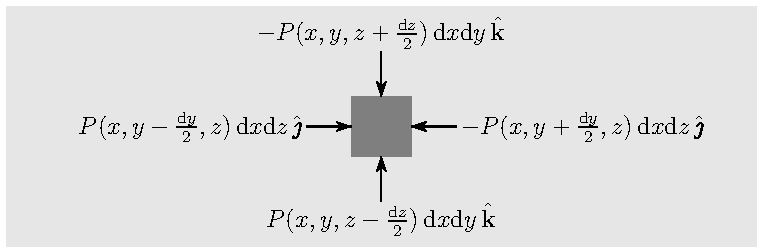
\includegraphics{fluidcube.pdf}
\end{center}
\end{efig}
The total force due to the pressure acting on the cube
is the sum 
\begin{align*}
&-P\left(x+\frac{\dee{x}}{2},y,z\right)\,dy\dee{z}\,\hi
+P\left(x-\frac{\dee{x}}{2},y,z\right)\,dy\dee{z}\,\hi\\
&-P\left(x,y+\frac{dy}{2},z\right)\,\dee{x}\dee{z}\,\hj
+P\left(x,y-\frac{dy}{2},z\right)\,\dee{x}\dee{z}\,\hj\\
&-P\left(x,y,z+\frac{\dee{z}}{2}\right)\,\dee{x}dy\,\hk
+P\left(x,y,z-\frac{\dee{z}}{2}\right)\,\dee{x}dy\,\hk
\end{align*}
of the forces acting on the six faces.
Consider the $\hi$ component and rewrite it as
\begin{align*}
&-P\left(x+\frac{\dee{x}}{2},y,z\right)\,dy\dee{z}\,\hi
+P\left(x-\frac{\dee{x}}{2},y,z\right)\,dy\dee{z}\,\hi \\
&\hskip1in
=-\frac{P(x+{\dee{x}\over2},y,z)-P(x-{\dee{x}\over2},y,z)}{\dee{x}}\,\hi\ 
     \dee{x} \dee{y} \dee{z} \\
&\hskip1in
= - \frac{\partial P}{\partial x}(x,y,z)\,\hi\ 
     \dee{x} \dee{y} \dee{z}
\end{align*}
%and rewriting the remaining four terms in a similar manner, we see that
Doing this for the other components as well,
we see that the total force due to the pressure acting on the cube is
\begin{align*}
-\Big\{\frac{\partial P}{\partial x}(x,y,z)\,\hi
+\frac{\partial P}{\partial y}(x,y,z)\,\hj
+\frac{\partial P}{\partial z}(x,y,z)\,\hk
\Big\}\dee{x} \dee{y} \dee{z}
=-\vnabla P(x,y,z)\, \dee{x} \dee{y} \dee{z}
\end{align*}
We shall assume that the only other force acting on the cube is gravity
and that the fluid is stationary (or at least not accelerating).
Hence the total force acting on the cube is zero. If the fluid has density
$\rhof$, then the  cube has mass $\rhof\, \dee{x}\dee{y}\dee{z}$ so that the force of 
gravity is $- g\rhof\,  \dee{x}\dee{y}\dee{z}\,\hk$. The vanishing of 
the total force now tells us that
\begin{equation*}
-\vnabla P(\vr)\, \dee{x} \dee{y} \dee{z}
- g\rhof\,  \dee{x} \dee{y} \dee{z}\,\hk=0
\implies \vnabla P(\vr)= - g\rhof  \,\hk
\end{equation*}
Subbing this into \eqref{eq:buoyancy} gives
\begin{equation*}
\vB= g\,\hk\tripInt_{V}\rhof\,\dee{V} = gM_f\,\hk
\end{equation*}
where $M_f =\tripInt_V \rhof\,\dee{V}$ is the mass of the fluid 
displaced by the object --- \emph{not} the mass of the object itself. 
Thus the buoyant force acts straight up and has magnitude equal to
$gM_f $, which is also the magnitude of the force of gravity acting on the 
fluid displaced by the object. In other words, it is the weight of the 
displaced fluid. This is exactly Archimedes' principle. 

We next consider the rotational motion of our submerged object. The physical
law that determines the rotational motion of a rigid body about a point
$\vr_0$ is analogous to the familiar Newton's law, $m\frac{d\vv}{\dee{t}}=\vF$, 
that determines the translational motion of the object. For the rotational
law of motion, 
\begin{itemize}\itemsep1pt \parskip0pt \parsep0pt %\itemindent-15pt
\item[$\circ$]
the mass $m$ is replaced by a physical quantity, characteristic
of the object, called the moment of inertia, and
\item[$\circ$] 
the ordinary velocity $\vv$ is replaced by the angular 
velocity, which is a vector whose length is the rate of rotation (i.e.
angle rotated per unit time) and whose direction is parallel to the axis
of rotation (with the sign determined by a right hand rule), and 
\item[$\circ$] the force $\vF$ 
is replaced by a vector called the torque about $\vr_0$.  A force $\vF$ applied 
at $\vr=(x,y,z)$ produces the torque\footnote{This is what Archimedes was referring to when he said ``Give me a lever and a place to stand and I will move the earth.''} $(\vr-\vr_0)\times\vF$ about $\vr_0$. 
\end{itemize}
This is derived in the optional \S\ref{sec:torque}, entitled ``Torque'', 
and is all that we need to know about rotational motion of rigid bodies in 
this discussion.

Fix any point $\vr_0$. The total torque about $\vr_0$ produced by 
force of pressure acting on the surface of the submerged object is
\begin{equation*}
\vT=\dblInt_{\partial V} (\vr-\vr_0)\times\big(-p(\vr)\hn\big)\,\dee{S}
=\dblInt_{\partial V} \hn\times\big(P(\vr)\, (\vr-\vr_0)\big)\,\dee{S}
\end{equation*}
Recall that in these integrals $\vr=(x,y,z)$ is the position of the 
infinitesimal piece $\dee{S}$ of the surface $S$.
Applying the cross product variant of the divergence theorem in Theorem
\ref{thm:divVrn}, followed by the vector identity 
Theorem \ref{thm:curlIdentities}.c, gives
\begin{align*}
\vT&=\tripInt_V \vnabla\times\big(P(\vr)\,(\vr-\vr_0)\big)\,\dee{V}
=\tripInt_V \big\{\vnabla P(\vr)\times(\vr-\vr_0)
     +P(\vr)\underbrace{\vnabla\times(\vr-\vr_0)}_{=\vZero}\big\}\,\dee{V}\cr
&=\tripInt_V \vnabla P(\vr)\times(\vr-\vr_0)\,\dee{V}
\end{align*}
since $\vnabla\times\vr_0=0$, because $\vr_0$ is a constant, and
\begin{equation*}
\vnabla\times\vr=\det\left[\begin{matrix}
                   \hi&\hj&\hk\cr
                   \frac{\partial\hfill}{\partial x}&
                   \frac{\partial\hfill}{\partial y}&
                   \frac{\partial\hfill}{\partial z}\\
                   x&y&z
                  \end{matrix}\right] 
=0
\end{equation*}
We have already found that $\vnabla P(\vr)=-g\rhof\hk$.
Substituting it in gives
\begin{alignat*}{3}
\vT&=-\tripInt_V g\rhof\hk\times(\vr-\vr_0)\,\dee{V}
&&=-g\hk\times\tripInt_V \rhof (\vr-\vr_0)\,\dee{V}\\
&=-g\hk\times\bigg\{\tripInt_V\! \vr\rhof\,\dee{V}
                 -\vr_0\!\tripInt_V\! \rhof\,\dee{V}\bigg\}
&&=-g\bigg\{\tripInt_V\! \rhof\,\dee{V}\bigg\}\hk\times \bigg\{
     \frac{\tripInt_V \vr\rhof\,\dee{V}}{\tripInt_V\rhof\,
                     \dee{V}}-\vr_0\bigg\}\\
&=-\vB\times\bigg\{\frac{\tripInt_V \vr\rhof\,\dee{V}}
                        {\tripInt_V\rhof\,\dee{V}}-\vr_0\bigg\}
&&=\bigg\{\frac{\tripInt_V \vr\rhof\,\dee{V}}
            {\tripInt_V\rhof\,\dee{V}}-\vr_0\bigg\}\times\vB
\end{alignat*}
So the torque generated at $\vr_0$ by pressure over the entire surface
is the same as the torque generated at $\vr_0$ by a force $\vB$ applied at the single point
\begin{equation*}
\vC_\vB=\frac{\tripInt_V \vr\rhof\,\dee{V}}{\tripInt_V\rhof\,\dee{V}}
\end{equation*}
This point is called the centre of buoyancy. It is the centre of mass
of the displaced fluid. 

%\noindent
The moral of the above discussion is that the buoyant force, $\vB$,
on a rigid body
\begin{itemize}\itemsep1pt \parskip0pt \parsep0pt %\itemindent-15pt
\item[$\circ$]
acts straight upward, 
\item[$\circ$] 
has magnitude equal to the weight of the displaced fluid and 
\item[$\circ$] 
acts at the centre of buoyancy, which is the centre of mass 
of the displaced fluid. 
\end{itemize}
As above, denoting by $\rhob$ the density of the object, 
the torque about $\vr_0$ due to gravity acting on the object is
\begin{equation*}
\tripInt_V (\vr-\vr_0)\times(-g\rhob\hk)\,\dee{V}
=\bigg\{\frac{\tripInt_V \vr\rhob\,\dee{V}}
            {\tripInt_V\rhob\,\dee{V}}-\vr_0\bigg\}\times
                  \left(-g\bigg\{\tripInt_V \rhob\,\dee{V}\bigg\}\ \hk\right)
\end{equation*}
So the gravitational force, $\vG$, 
\begin{itemize}\itemsep1pt \parskip0pt \parsep0pt %\itemindent-15pt
\item[$\circ$]
acts straight down, 
\item[$\circ$] 
has magnitude equal to the weight 
$g M_b=g\tripInt_V \vr\rhob\,\dee{V}$ (where $\rhob$ is the density of 
the object) of the object and 
\item[$\circ$] 
acts at the centre of mass,
$
\vC_\vG=\frac{\tripInt_V \vr\rhob\,\dee{V}}{\tripInt_V\rhob\,\dee{V}}
$, 
of the object.
\end{itemize}
\intremark{
The torque about $\vr_0$ due to gravity is
\begin{alignat*}{3}
\vT&=-\tripInt_V (\vr-\vr_0)\times g\rhob\hk\,\dee{V}
&&=g\hk\times\tripInt_V \rhob (\vr-\vr_0)\,\dee{V}\\
&=g\hk\times\bigg\{\tripInt_V\! \vr\rhob\,\dee{V}
                 -\vr_0\!\tripInt_V\! \rhob\,\dee{V}\bigg\}
&&=g\bigg\{\tripInt_V\! \rhob\,\dee{V}\bigg\}\hk\times \bigg\{
     \frac{\tripInt_V \vr\rhob\,\dee{V}}{\tripInt_V\rhob\,\dee{V}}-\vr_0\bigg\}
\\
&=\big(gM_b\hk\big)\times\bigg\{\frac{\tripInt_V \vr\rhob\,\dee{V}}
                        {\tripInt_V\rhob\,\dee{V}}-\vr_0\bigg\}
&&=\bigg\{\frac{\tripInt_V \vr\rhob\,\dee{V}}
            {\tripInt_V\rhob\,\dee{V}}-\vr_0\bigg\}\times\big(-gM_b\hk\big)
\end{alignat*}


}

\noindent
Because the mass distribution of the object need not be the same as the
mass distribution of the displaced fluid, buoyancy and gravity may act at 
two different points. This is exploited in the design of self-righting boats.
 
These boats are constructed with a heavy, often lead (which is cheap and dense), keel.  As a result, the centre of gravity is lower in the boat 
than the center of buoyancy, which, because the displaced fluid has constant density, is at the geometric centre of the boat. As the figure below illustrates, 
a right side up configuration of such a boat is stable, while an upside down 
configuration is unstable. The boat rotates so as to keep the centre
of gravity straight below the centre of buoyancy. To see this pretend that
you are holding on to the boat with one hand holding the centre of buoyancy
and the other hand holding the centre of gravity. Use your hands to apply forces
in the directions of the arrows and think about how the boat will respond.

\begin{efig}
\begin{center}
    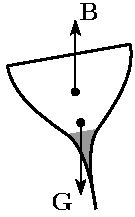
\includegraphics{boatU.pdf}\qquad\qquad\qquad
    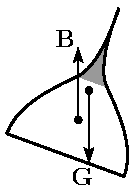
\includegraphics{boatD.pdf}
\end{center}
\end{efig}

%%%%%%%%%%%%%%%%%
\subsection{Optional --- Torque}\label{sec:torque}
%%%%%%%%%%%%%%%%%

In this section, we derive the properties of torque that we used in 
the last section. Newton's law of motion says that the position $\vr(t)$ 
of a single particle moving under the influence
of a force $\vF$ obeys $m\vr''(t)=\vF$. Similarly, the positions $\vr_i(t)$, 
$1\le i\le n$, of a set of particles moving under the influence
of forces $\vF_i$ obey $m\vr_i''(t)=\vF_i$, $1\le i\le n$. Very often 
systems of interest consist
of some small number of rigid bodies. Suppose that we are interested in
the motion of a single rigid body, say a piece of wood. The piece of wood
is made up of a huge number\footnote{Just 12 grams of carbon contains
about $6\times 10^{23}$ atoms.} of atoms. So the system of equations 
determining the motion of all of the individual atoms in the piece of 
wood is huge. On the other hand, we shall see that because the piece of 
wood is rigid, its configuration is completely determined by the 
position of, for example, its centre of mass and its orientation 
(we won't get into what precisely is meant by ``orientation'', but 
it is certainly determined by, for example, the positions of a few 
of the corners of the piece of wood). 
To be precise, we shall extract from the  huge system of equations 
that determine the motion of all of the individual atoms, a 
small system of equations that determine the motion of the centre of mass 
and the orientation. We'll do so now.

Imagine a piece of wood moving in $\bbbr^3$.
\vadjust{
\begin{nfig}
\begin{center}
    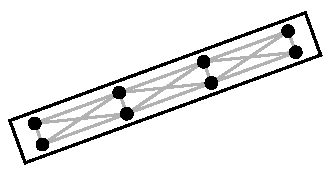
\includegraphics{seesaw.pdf}
\end{center}
\end{nfig}
}
Furthermore, imagine that the piece of wood consists of a huge number of
particles joined by a huge number of weightless but very 
strong\footnote{Mathematicians and their idealizations! Really the rods just
represent the atomic/chemical forces that hold the wood together.} steel rods.
The steel rod joining particle number one to particle number two just
represents a force acting between particles number one and two.
Suppose that
\begin{itemize}\itemsep1pt \parskip0pt \parsep0pt %\itemindent-15pt
\item[$\circ$] 
there are $n$ particles, with particle number $i$ having mass $m_i$,
\item[$\circ$] 
at time $t$, particle number $i$ has position $\vr_i(t)$,
\item[$\circ$] 
at time $t$,  the external force (gravity and the like)
acting on particle number $i$ is $\vF_i(t)$, and
\item[$\circ$] 
at time $t$, the force acting on particle number $i$,
due to the steel rod joining particle number $i$ to particle number $j$
is $\vF_{i,j}(t)$. If there is no steel rod joining particles 
number $i$ and $j$, just set
$\vF_{i,j}(t)=0$. In particular, $\vF_{i,i}(t)=0$.
\end{itemize}
The only assumptions that we shall make about the steel rod forces are
\begin{itemize}\itemsep1pt \parskip0pt \parsep0pt %\itemindent-15pt
\item[(A1)]
for each $i\ne j$, $\vF_{i,j}(t)=-\vF_{j,i}(t)$. In words, 
the steel rod joining particles $i$ and $j$ applies equal and opposite 
forces to particles $i$ and $j$.
\item[(A2)] 
for each $i\ne j$, there is a function $M_{i,j}(t)$ such
that $\vF_{i,j}(t)=M_{i,j}(t)\big[\vr_i(t)-\vr_j(t)\big]$. In words, 
the force due to the rod joining particles $i$ and $j$ acts parallel to the 
line joining particles $i$ and $j$. For (A1) to be true, that is 
to have $M_{i,j}(t)\big[\vr_i(t)-\vr_j(t)\big]
=-M_{j,i}(t)\big[\vr_j(t)-\vr_i(t)\big]$, we need 
$M_{i,j}(t)=M_{j,i}(t)$.
\end{itemize}
Newton's law of motion, applied to particle number $i$,  now tells us that
\begin{align}
m_i \vr''_i(t)&= \vF_i(t)+\sum_{j=1}^n \vF_{i,j}(t)
%\tag{\ref{eqn:rigid}$_i$}\end{align}
\tag{$N_i$}\end{align}
Adding up all of the equations ($N_i$), 
for $i=1,\ 2,\ 3,\ \cdots,\ n$ gives
\begin{align}
\sum_{i=1}^n m_i \vr''_i(t)&= \sum_{i=1}^n \vF_i(t)+\sum_{1\le i,j\le n} \vF_{i,j}(t)
\tag{$\Sigma N_i$}\end{align}
The sum $\sum\limits_{1\le i,j\le n} \vF_{i,j}(t)$ contains $\vF_{1,2}(t)$
exactly once and it also contains $\vF_{2,1}(t)$ exactly once and these two
terms cancel exactly, by assumption (A1). In this way, all terms in 
$\sum\limits_{1\le i,j\le n} \vF_{i,j}(t)$
with $i\ne j$ exactly cancel. All terms with $i=j$ are assumed to be zero.
So $\sum\limits_{1\le i,j\le n} \vF_{i,j}(t)=0$ and the equation 
($\Sigma N_i$) simplifies to
\begin{align}
\sum_{i=1}^n m_i \vr''_i(t)&= \sum_{i=1}^n \vF_i(t)
\tag{$\Sigma N_i$}\end{align}
Phew! Denote by $M=\sum\limits_{i=1}^n m_i$ the total mass of the body,
by $\vR(t)=\frac{1}{M}\sum\limits_{i=1}^n m_i\vr_i(t)$  the centre of 
mass\footnote{Note that this is just the weighted average (no pun intended)
of the positions of the particles.} of the body and by 
$\vF(t)=\sum\limits_{i=1}^n \vF_i(t)$  the total external force acting
on the system. In this notation, equation ($\Sigma N_i$) can be written as
\begin{impeqn}\label{eqn:rigidCofM}
\begin{equation*}
M\vR''(t)=\vF(t)
\end{equation*}
\end{impeqn}
\noindent 
The upshot is that the centre of mass of the system moves just like 
a single particle of mass $M$ subject to the total external force.
This is why we can often replace an extended object by a point mass at its
centre of mass.

Now take the cross product of $\vr_i(t)$ and equation ($N_i$) 
and sum over $i$. This gives
\begin{equation}
\sum_{i=1}^n m_i\ \vr_i(t)\times\vr''_i(t)
= \sum_{i=1}^n \vr_i(t)\times\vF_i(t)
+\sum_{1\le i,j\le n} \vr_i(t)\times\vF_{i,j}(t)
\tag{$\Sigma \vr_i\times N_i$}\end{equation}
By the assumption (A2)
\begin{align*}
\vr_1(t)\times\vF_{1,2}(t)
&=M_{1,2}(t)\ \vr_1(t)\times\big[\vr_1(t)-\vr_2(t)\big]\\
%%%
\vr_2(t)\times\vF_{2,1}(t)
&=M_{2,1}(t)\ \vr_2(t)\times\big[\vr_2(t)-\vr_1(t)\big]\\
&=-M_{1,2}(t)\ \vr_2(t)\times\big[\vr_1(t)-\vr_2(t)\big]\\
\intertext{so that}
\vr_1(t)\times\vF_{1,2}(t)
+\vr_2(t)\times\vF_{2,1}(t)
&=M_{1,2}(t)\ \big[\vr_1(t)-\vr_2(t)\big]\times\big[\vr_1(t)-\vr_2(t)\big]
=0
\end{align*}
because the cross product of any two parallel vectors is zero.

The last equation says that the $i=1$, $j=2$ term in 
$\sum\limits_{1\le i,j\le n} \vr_i(t)\times\vF_{i,j}(t)$
exactly cancels the $i=2$, $j=1$ term. 
In this way all of the terms in 
$\sum\limits_{1\le i,j\le n} \vr_i(t)\times\vF_{i,j}(t)$
with $i\ne j$ cancel. Each term with $i=j$ is exactly zero because
$\vF_{ii}=0$.
So $\sum\limits_{1\le i,j\le n} \vr_i(t)\times\vF_{i,j}(t)=0$
and ($\Sigma \vr_i\times N_i$) simplifies to
\begin{equation}
\sum_{i=1}^n m_i\ \vr_i(t)\times\vr''_i(t)
= \sum_{i=1}^n \vr_i(t)\times\vF_i(t)
\tag{$\Sigma \vr_i\times N_i$}\end{equation}
At this point it makes sense to define vectors
\begin{align*}
\vL(t)&= \sum_{i=1}^n m_i\ \vr_i(t)\times\vr'_i(t)\\
\vT(t)&=\sum_{i=1}^n \vr_i(t)\times\vF_i(t)
\end{align*}
because, in this notation, ($\Sigma \vr_i\times N_i$) becomes
\begin{impeqn}\label{eqn:rigidR}
\begin{equation*}
\diff{\hfill}{t}\vL(t)=\vT(t)
\end{equation*}
\end{impeqn}
\noindent
Equation \eqref{eqn:rigidR} plays the r\^ole of Newton's law of 
motion for rotational motion. $\vT(t)$ is called the torque and 
plays the r\^ole of ``rotational force''. $\vL(t)$ is called the 
angular momentum (about the origin) and is a measure of the rate 
at which the piece of wood is rotating. 
For example, if a particle of mass $m$ is traveling in a circle of 
radius $\rho$ in the $xy$-plane at $\om$ radians per unit time, then $\vr(t)=\rho\cos(\om t)\hi+\rho\sin(\om t)\hj$ and
\begin{align*}
m\vr(t)\times\vr'(t) 
&= m \big[\rho\cos(\om t)\hi+\rho\sin(\om t)\hj\big]
\times\big[-\om\rho\sin(\om t)\hi+\om\rho\cos(\om t)\hj\big] \\
&=m \rho^2\ \om\ \hk
\end{align*}
is proportional to $\om$, which is the rate of rotation about the origin
and is in the direction $\hk$, which is normal to the plane containing
the circle.

In any event, in order for the piece of wood to remain stationary, 
equations \eqref{eqn:rigidCofM} and \eqref{eqn:rigidR} 
force $\vF(t)=\vT(t)=0$.

Now suppose that the piece of wood is a seesaw\footnote{Or teeter-totter
for those who speak a different English dialect.} that is supported on a 
fulcrum at $\vp$. The forces consist of gravity, $-m_ig\hk$,
acting on particle number $i$, for each  $1\le i\le n$, and the% 
\vadjust{
\begin{nfig}
\begin{center}
    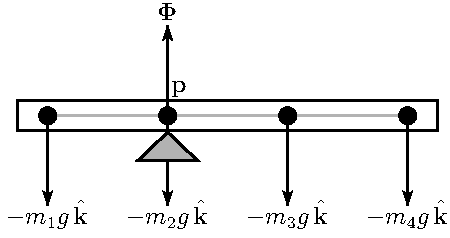
\includegraphics{seesaw2.pdf}
\end{center}
\end{nfig}
}
force $\vPhi$ imposed by the fulcrum that is pushing up on the particle 
at $\vp$. The total external force is $\vF=\vPhi-\sum\limits_{i=1}^n m_ig\hk
=\vPhi-Mg\hk$. If the seesaw is to remain stationary, this must be zero so that
$\vPhi=Mg\hk$. 

The total torque (about the origin) is 
\begin{equation*}
\vT=\vp\times\vPhi-\sum_{i=1}^n m_ig \vr_i\times\hk
=g\Big(M\vp-\sum_{i=1}^n m_i \vr_i\Big)\times\hk
\end{equation*}
If the seesaw is to remain stationary, this must also be zero. This will
be the case if the fulcrum is placed at
\begin{equation*}
\vp=\frac{1}{M}\sum_{i=1}^n m_i \vr_i
\end{equation*}
which is just the centre of mass of the piece of wood.

More generally, suppose that the external forces acting on the piece of wood
consist of $\vF_i$, acting on particle number $i$, for each $1\le i\le n$, 
and a ``fulcrum force'' $\vPhi$ acting on a particle at 
$\vp$. The total external force is $\vF=\vPhi+\sum\limits_{i=1}^n \vF_i$. 
If the piece of wood is to remain stationary, this must be zero so that
$\vPhi=-\sum\limits_{i=1}^n \vF_i$. The total torque (about the origin) is 
\begin{equation*}
\vT=\vp\times\vPhi+\sum_{i=1}^n \vr_i\times\vF_i
=\sum_{i=1}^n (\vr_i-\vp)\times\vF_i
\end{equation*}
If the piece of wood is to remain stationary, this must also be zero. 
That is, the torque about point $\vp$ due to all of the forces $\vF_i$,
$1\le i\le n$, must be zero.



%%%%%%%%%%%%%%%%%
\subsection{Optional --- Solving Poisson's Equation}\label{sec:poisson}
%%%%%%%%%%%%%%%%%

In this section we shall use the divergence theorem to find a formula for the solution of Poisson's equation
\begin{equation*}
\vnabla^2\varphi = 4\pi\rho
\end{equation*}
Here $\rho=\rho(\vr)$ is a given (continuous) function and $\varphi$ 
is the unknown function that we wish to find.
This equation arises, for example, in electrostatics, where $\rho$ is 
the charge density and $\varphi$ is the electric potential. 

The main step in finding this solution formula will be to consider an
\begin{itemize}\itemsep1pt \parskip0pt \parsep0pt \itemindent 15pt
\item[]
arbitrary (smooth) function $\varphi$ and an 
\item[]
arbitrary (smooth) region $V$  in $\bbbr^3$ and an
\item[]
arbitrary point $\vr_0$ in the interior of $V$
\end{itemize}
and to find an auxiliary formula which expresses $\varphi(\vr_0)$ in terms of 
\begin{itemize}\itemsep1pt \parskip0pt \parsep0pt \itemindent 15pt
\item[]
$\vnabla^2\varphi(\vr)$, with $\vr$ running over $V$ and
\item[]
$\vnabla\varphi(\vr)$ and $\varphi(\vr)$, with $\vr$ running only over 
$\partial V$.
\end{itemize}
This auxiliary formula, which we shall derive below, is
\begin{equation}
\varphi(\vr_0)=-\frac{1}{4\pi}\bigg\{
\tripInt_V\frac{ \vnabla^2\varphi(\vr)}{|\vr-\vr_0|}\ d^3\vr
-\dblInt_{\partial V}\varphi(\vr)\frac{\vr-\vr_0}{|\vr-\vr_0|^3}\cdot\hn\ \dee{S}
-\dblInt_{\partial V}\frac{\vnabla\varphi(\vr)}{|\vr-\vr_0|}\cdot\hn\ \dee{S}\bigg\}
\tag{$V$}
\end{equation}
When we take the limit as $V$ expands to fill all of $\bbbr^3$ then,
assuming that $\varphi$ and $\vnabla\varphi$ go to zero sufficiently 
quickly\footnote{Suppose, for example, that, for large $|\vr-\vr_0|$, 
$|\varphi(\vr)|$ is bounded by a constant times $\nicefrac{1}{|\vr-\vr_0|}$
and $|\vnabla\varphi(\vr)|$ is bounded by a constant times 
$\nicefrac{1}{|\vr-\vr_0|^2}$. Then, if $\partial V$ is the sphere of 
radius $R$ centred on $\vr_0$,  $\partial V$ has surface area $4\pi R^2$ 
and the two integrals over $\partial V$ are bounded by a constant times
$\nicefrac{1}{R}$.}
at $\infty$, the two integrals over $\partial V$ will converge to zero and
we will end up with the formula 
\begin{equation*}
\varphi(\vr_0)=-\frac{1}{4\pi}
\tripInt_{\bbbr^3}\frac{ \vnabla^2\varphi(\vr)}{|\vr-\vr_0|}\ d^3\vr
\end{equation*}
This expresses $\varphi$ evaluated at an
arbitrary point, $\vr_0$, of $\bbbr^3$ in terms of $\vnabla^2\varphi(\vr)$, 
with $\vr$ running over $\bbbr^3$, which is exactly what we want, since
$\vnabla^2\varphi = 4\pi\rho$ for any solution of Poisson's equation.
So once we have proven (V) we will have proven\footnote{Note that the theorem
does not claim that the $\varphi$ defined in the theorem obeys
$\vnabla^2\varphi = 4\pi\rho$. It does, but the proof is beyond our scope.}
\begin{theorem}\label{thm:PoissonSoln}
Assume that $\rho(\vr)$ is continuous and decays sufficiently quickly as
$\vr\rightarrow\infty$.  If $\varphi$ obeys
$\vnabla^2\varphi = 4\pi\rho$ on $\bbbr^3$, and $\varphi$ 
and $\vnabla\varphi$ decay sufficiently quickly as $\vr\rightarrow\infty$, then
\begin{equation*}
\varphi(\vr_0)=
-\tripInt_{\bbbr^3}\frac{ \rho(\vr)}{|\vr-\vr_0|}\ d^3\vr
\end{equation*}
for all $\vr_0$ in $\bbbr^3$.
\end{theorem}

Let 
\begin{align*}
\vr(x,y,z)&=x\,\hi+y\,\hj+z\,\hk\\
\vr_0&=x_0\,\hi+y_0\,\hj+z_0\,\hk
\end{align*}
We shall exploit three properties of the function
$\frac{1}{|\vr-\vr_0|}$. The first two properties are
\begin{align}
\vnabla \frac{1}{|\vr-\vr_0|} &=-\frac{\vr-\vr_0}{|\vr-\vr_0|^3}\tag{P1}\\
\vnabla^2 \frac{1}{|\vr-\vr_0|} &=-\vnabla\cdot\frac{\vr-\vr_0}{|\vr-\vr_0|^3}
=0
\tag{P2}\end{align}
and are valid for all $\vr\ne \vr_0$. Verification of the first property is
a simple one line computation. Verification of the second property is
a simple three line computation. (See the solution to Question 
\eref{PROB4}{poisson} in Section 4.1 of the CLP-4 problem book.)

The other property of $\frac{1}{|\vr-\vr_0|}$ 
that we shall use is the following. Let $S_\veps$ be the sphere of 
radius $\veps$ centered on $\vr_0$. Then, for any continuous function $\psi(\vr)$,
\begin{align}
\lim_{\veps\rightarrow 0+}\dblInt_{S_\veps}
              \frac{\psi(\vr)}{|\vr-\vr_0|^p}\ \dee{S}
&=\lim_{\veps\rightarrow 0+} \frac{1}{\veps^p} \dblInt_{S_\veps}
              \psi(\vr)\ \dee{S}
=\lim_{\veps\rightarrow 0+}\frac{\psi(\vr_0)}{\veps^p}
             \dblInt_{S_\veps}\ \dee{S}
=\lim_{\veps\rightarrow 0+}\frac{\psi(\vr_0)}{\veps^p}4\pi\veps^2
\notag\\
&=\begin{cases}4\pi\psi(\vr_0)& \text{if $p=2$}\\
         0             & \text{if $p<2$}\\
         \text{undefined} & \text{if $p>2$}
         \end{cases}
\tag{P3}
\end{align}

\intremark{

\noindent
Here is the verification of (P1) and (P2). 
It suffices to consider $\vr_0=\vZero$.
The $x$-component of (P1) is
\begin{align*}
\frac{\partial\hfill}{\partial x}\frac{1}{|\vr|}
=\frac{\partial\hfill}{\partial x}\frac{1}{\sqrt{x^2+y^2+z^2}}
=-\frac{1}{2}\frac{2x}{{\big[x^2+y^2+z^2\big]}^{3/2}}
=-\frac{\vr\cdot\hi}{|\vr|^3}
\end{align*}
as desired. For (P2), we have
\begin{align*}
\vnabla\cdot\frac{\vr}{|\vr|^3}
&=\frac{\partial\hfill}{\partial x}\frac{x}{{\big[x^2+y^2+z^2\big]}^{3/2}}
+\frac{\partial\hfill}{\partial y}\frac{y}{{\big[x^2+y^2+z^2\big]}^{3/2}}
+\frac{\partial\hfill}{\partial z}\frac{z}{{\big[x^2+y^2+z^2\big]}^{3/2}}
\\
&=\frac{\big[x^2+y^2+z^2\big]-x\frac{3}{2}(2x)}{{\big[x^2+y^2+z^2\big]}^{5/2}}
+\frac{\big[x^2+y^2+z^2\big]-y\frac{3}{2}(2y)}{{\big[x^2+y^2+z^2\big]}^{5/2}}
+\frac{\big[x^2+y^2+z^2\big]-z\frac{3}{2}(2z)}{{\big[x^2+y^2+z^2\big]}^{5/2}}
\\
&=0
\end{align*}

}


\noindent\emph{Derivation of (V):}

Here is the derivation of ($V$). Let $V_\veps$ be the part of $V$ outside
of $S_\veps$. 
\vadjust{
\begin{nfig}
\begin{center}
    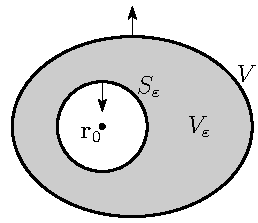
\includegraphics{poisson.pdf}
\end{center}
\end{nfig}
}
Note that the boundary $\partial V_\veps$ of $V_\veps$ consists
of two parts --- the boundary $\partial V$ of $V$ and the sphere $S_\veps$
--- and that the unit outward normal to $\partial V_\veps$ on $S_\veps$ is
$-\frac{\vr-\vr_0}{|\vr-\vr_0|}$, because it points towards $\vr_0$ and hence
outside of $V_\veps$.


Recall the vector identity Theorem \ref{thm:degTwoIdentities}.d, which says
\begin{equation*}
\vnabla\cdot(f\vnabla g-g\vnabla f)=f\,\vnabla^2g-g\,\vnabla^2f
\end{equation*}
Applying this identity with $f= \frac{1}{|\vr-\vr_0|}$ and $g=\varphi$
gives
\begin{align*}
\vnabla\cdot\Big(\frac{1}{|\vr-\vr_0|}\vnabla\varphi
-\varphi\vnabla\frac{1}{|\vr-\vr_0|}\Big)
&=\frac{\vnabla^2\varphi}{|\vr-\vr_0|}
  -\varphi\,\overbrace{ \vnabla^2\frac{1}{|\vr-\vr_0|} }^{=0\text{ by (P2)}} \\
&=\frac{\vnabla^2\varphi}{|\vr-\vr_0|}
\end{align*}
which is the integrand of the first integral on the right hand side of (V). 
So, by the divergence theorem
\begin{align}
\tripInt_{V_\veps} \frac{\vnabla^2\varphi}{|\vr-\vr_0|} dV
&=\tripInt_{V_\veps}\vnabla\cdot\Big(\frac{1}{|\vr-\vr_0|}\vnabla\varphi
-\varphi\vnabla\frac{1}{|\vr-\vr_0|}\Big) dV \notag\\
&=\dblInt_{\partial V}\Big(\frac{1}{|\vr-\vr_0|}\vnabla\varphi
-\varphi\vnabla\frac{1}{|\vr-\vr_0|}\Big)\cdot\hn\ \dee{S}  \notag\\
&\hskip1in+\dblInt_{S_\veps}\Big(\frac{1}{|\vr-\vr_0|}\vnabla\varphi
-\varphi\vnabla\frac{1}{|\vr-\vr_0|}\Big)\cdot
\Big(-\frac{\vr-\vr_0}{|\vr-\vr_0|}\Big) \dee{S}
\tag{M}\end{align}
To see the connection between (M) and the rest of (V), note that, 

\begin{itemize}\itemsep1pt \parskip0pt \parsep0pt %\itemindent-15pt
\item[$\circ$]
by (P1), the first term on the right hand side of (M) is
\begin{equation}
\dblInt_{\partial V}\Big(\frac{1}{|\vr-\vr_0|}\vnabla\varphi
-\varphi\vnabla\frac{1}{|\vr-\vr_0|}\Big)\cdot\hn\ \dee{S}
=\dblInt_{\partial V}\frac{\vnabla\varphi(\vr)}{|\vr-\vr_0|}\cdot\hn\ \dee{S}
+\dblInt_{\partial V}\varphi(\vr)\frac{\vr-\vr_0}{|\vr-\vr_0|^3}\cdot\hn\ \dee{S}
\tag{R1}\end{equation}
which is $4\pi$ times the second and third terms on the right hand side of (V),
%\item[$\circ$]
%So applying $\lim_{\veps\rightarrow 0+}$ to to the left hand side of (M) 
%gives
%\begin{equation}
%\lim_{\veps\rightarrow 0+}
%\tripInt_{V_\veps}\vnabla\cdot\Big(\frac{1}{|\vr-\vr_0|}\vnabla\varphi
%-\varphi\vnabla\frac{1}{|\vr-\vr_0|}\Big) dV
%=\tripInt_{V}\frac{\vnabla^2\varphi}{|\vr-\vr_0|}\ dV
%\tag{L}\end{equation}


\item[$\circ$]
and substituting in 
$\vnabla \frac{1}{|\vr-\vr_0|} =-\frac{\vr-\vr_0}{|\vr-\vr_0|^3}$,
from (P1), and applying (P3) with $p=2$, the limit of the second 
term on the right hand side of (M) is
\begin{align}
&\lim_{\veps\rightarrow 0+}
\dblInt_{S_\veps}\Big(\frac{1}{|\vr-\vr_0|}\vnabla\varphi
-\varphi\vnabla\frac{1}{|\vr-\vr_0|}\Big)\cdot
        \Big(-\frac{\vr-\vr_0}{|\vr-\vr_0|}\Big) \dee{S}
\notag\\
&\hskip1in=-\lim_{\veps\rightarrow 0+}
\dblInt_{B_\veps}\big[\vnabla\varphi\cdot(\vr-\vr_0)+\varphi\big]
\frac{1}{|\vr-\vr_0|^2} \dee{S}
\notag\\
&\hskip1in=-4\pi\Big[\vnabla\varphi\cdot(\vr-\vr_0)+\varphi\Big]_{\vr=\vr_0}
\notag\\
&\hskip1in=-4\pi\varphi(\vr_0)
\tag{R2}\end{align}
\end{itemize}
So applying\footnote{You might worry about the singularity in 
$\frac{\vnabla^2\varphi}{|\vr-\vr_0|}$
when applying $\lim_{\veps\rightarrow 0+}$ to $\tripInt_{V_\veps} \frac{\vnabla^2\varphi}{|\vr-\vr_0|} dV$. That this singularity 
is harmless may be seen using spherical coordinates centred on $\vr_0$.
Then $\dee{V}$ contains a factor of $|\vr-\vr_0|^2$ 
(see \S\ref{ap:spherCoord}), 
which completely eliminates the singularity. 
}
$\lim_{\veps\rightarrow 0+}$ to (M) and substituting in (R1) and (R2) 
gives
\begin{align*}
\tripInt_{V}\frac{\vnabla^2\varphi}{|\vr-\vr_0|}\ dV
=\dblInt_{\partial V}\frac{\vnabla\varphi(\vr)}{|\vr-\vr_0|}\cdot\hn\ \dee{S}
+\dblInt_{\partial V}\varphi(\vr)\frac{\vr-\vr_0}{|\vr-\vr_0|^3}\cdot\hn\ \dee{S}
-4\pi\varphi(\vr_0)
\end{align*}
which is exactly equation (V).


%\newpage
%%%%%%%%%%%%%%%%%%%%%%%%%
\section{Green's Theorem}\label{sec:GreenThm}
%%%%%%%%%%%%%%%%%%%%%%%%%%
Our next variant of the fundamental theorem of calculus is 
Green's\footnote{George Green (1793--1841) was a British 
mathematical physicist. He spent much of the early part of his life
working in his father's bakery and grain mill. He was finally admitted
as an undergraduate to Cambridge in 1832, aged nearly forty.} theorem, which 
relates an integral, of a derivative of a (vector-valued) function,
over a region  in the $xy$-plane, with an integral of the function
over the curve bounding the region. 
First we need to define some properties of curves.

\begin{defn}\label{def:Green}

\begin{enumerate}[(a)]
\item 
A curve $C$ with parametrization $\vr(t)$, $a\le t\le b$, is said to be 
\emph{closed} if $\vr(a)=\vr(b)$.

\item 
A curve $C$ is said to be \emph{simple} if it does not cross itself.
More precisely, if $\vr(t)$, $a\le t\le b$, is a parametrization of the
curve and if $a\le t_1,t_2\le b$ obey $t_1\ne t_2$ and $\{t_1,t_2\}
\ne\{a,b\}$, then $\vr(t_1)\ne \vr(t_2)$. That is, if $\vr(t_1)=\vr(t_2)$,
then either $t_1=t_2$ or $t_1=a$, $t_2=b$, or $t_1=b$, $t_2=a$.

\item 
A curve $C$ is \emph{piecewise smooth} if it has a parametrization
$\vr(t)$ which
\begin{itemize}  \itemsep1pt \parskip0pt \parsep0pt %\itemindent-15pt
\item
is continuous and which
\item
is differentiable except possibly at finitely many points with
\item
the derivative being continuous and nonzero except possibly at finitely 
many points.
\end{itemize}
\end{enumerate}
\end{defn}
\noindent Here are sketches of some examples.

\begin{wfig}
\begin{center}
    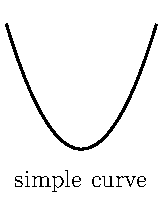
\includegraphics{curve1.pdf}\qquad
    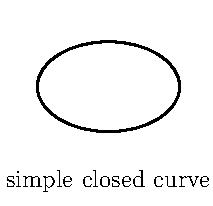
\includegraphics{curve2.pdf}\qquad
    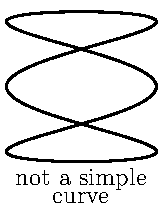
\includegraphics{curve3.pdf}\qquad
    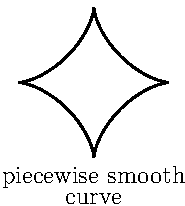
\includegraphics{astroid5.pdf}
\end{center}
\end{wfig}
And here is Green's theorem.

\begin{theorem}[Green's Theorem]\label{thm:Green}
Let 
\begin{itemize}\itemsep1pt \parskip0pt \parsep0pt % \itemindent-15pt
\item
$R$ be a finite region in the $xy$-plane,
\item
the boundary, $C$, of $R$ consist of a finite number of piecewise smooth, simple closed curves 
    \begin{itemize}\itemsep1pt \parskip0pt \parsep0pt %\itemindent-15pt
     \item
     that are oriented (i.e. arrows are put on $C$) consistently 
     with $R$ in the sense that if you walk along
     $C$ in the direction of the arrows, then $R$ is on your left
    \end{itemize}
     \begin{efig}
     \begin{center}
        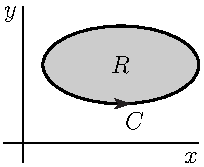
\includegraphics{greens1.pdf}\qquad
        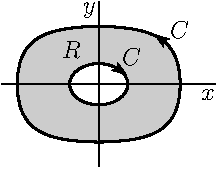
\includegraphics{dcircleE.pdf}
    \end{center}
    \end{efig}
\item
$F_1(x,y)$ and $F_2(x,y)$ have continuous first partial derivatives 
at \emph{every} point of $R$.
\end{itemize}
Then
\begin{equation*}
\oint_{C} \big[F_1(x,y)\,\dee{x} +F_2(x,y)\,\dee{y}\big]
 =\dblInt_{R}\left(\frac{\partial F_2}{\partial x} 
                - \frac{\partial F_1}{\partial y}\right)\ \dee{x}\dee{y}
\end{equation*}
\end{theorem}

\begin{warning}\label{warn:Green}
Note that in Theorem \ref{thm:Green} we are assuming that
$F_1$ and $F_2$ have continuous first partial derivatives 
at \emph{every} point of $R$.
If that is not the case, for example
because $F_1$ or $F_2$ is not defined on all of $R$, then 
the conclusion of Green's theorem can fail. An example is
$F_1=-\frac{y}{x^2+y^2}$, $F_2=\frac{x}{x^2+y^2}$, $R=\Set{(x,y)}{x^2+y^2\le 1}$.
See Examples~\ref{eg:greenC} and \ref{eg:greenCC}.
\end{warning}

\noindent
Here are three notational remarks before we start the proof.
\begin{itemize}\itemsep1pt \parskip0pt \parsep0pt \itemindent-15pt
\item[$\circ$]
One way to remember the integrand on the right hand side is to write it
as $(\vnabla\times\vF)\cdot\hk$.
\item[$\circ$]
Many people use $M$ instead of $F_1$ and $N$ instead of $F_2$.
Then Green's theorem becomes 
$\oint_{C} \big[M(x,y)\,\dee{x} +N(x,y)\,\dee{y}\big]
 =\dblInt_{R}\Big(\frac{\partial N}{\partial x} 
                - \frac{\partial M}{\partial y}\Big)\ \dee{x}\dee{y}$
\item[$\circ$] The symbol $\oint_C$ is just an alternate notation for $\int_C$
that is sometimes used when $C$ is a closed curve. 
See Notation \ref{not:workIntegral}.
\end{itemize}
\begin{proof}
We prove the result by reformulating it as a divergence theorem statement.
To that end, we define
\begin{align*}
V&=\Set{(x,y,z)}{ (x,y)\in R,\ \ 0\le z\le 1} \\
\vG(x,y,z) &= F_2(x,y)\,\hi -F_1(x,y)\,\hj
\end{align*}
Notice that $V$ is exactly the volume obtained by expanding $R$ vertically
upward by one unit.
 
\begin{nfig}
\begin{center}
    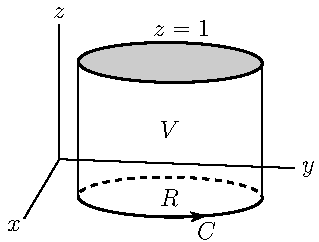
\includegraphics{greens2.pdf}
\end{center}
\end{nfig}
The definition of $\vG$ does \emph{not} contain a typo --- the $x$-component
of $\vG$ really is $F_2$ and the $y$-component of $\vG$ really is $-F_1$.
(More or less the reverse of what you would normally write down.)

These definitions have been rigged so that the divergence theorem
applied to $\vG$ and $V$, namely
\begin{align*}
\dblInt_{\partial V} \vG\cdot\hn\,\dee{S}
&=\tripInt_V\vnabla\cdot\vG\ \dee{V} 
\end{align*}
gives us exactly Green's theorem, as we shall now see.

Since $\vnabla\cdot\vG = \frac{\partial F_2}{\partial x} 
                - \frac{\partial F_1}{\partial y}$,  the right hand side is just
\begin{align*}
\tripInt_V\vnabla\cdot\vG\ \dee{V}
&= \dblInt_{R}\dee{x}\dee{y}\int_0^1\dee{z} \ \vnabla\cdot\vG \\
&= \dblInt_{R}\dee{x}\dee{y}\int_0^1\dee{z} \ 
        \left(\frac{\partial F_2}{\partial x}(x,y) 
                - \frac{\partial F_1}{\partial y}(x,y)\right) \\
&= \dblInt_{R}\dee{x}\dee{y}\
        \left(\frac{\partial F_2}{\partial x}(x,y) 
                - \frac{\partial F_1}{\partial y}(x,y)\right) 
\end{align*}
because the integrand is independent of $z$. This is exactly the right 
hand side of Green's theorem.

Now for the left hand side. The boundary, $\partial V$, of $V$ is the union 
of the (flat) bottom, the (flat) top and the (curved) side.
The outward unit normal on the (horizontal, flat) top is $+\hk$ and
the outward unit normal on the (horizontal, flat) bottom is $-\hk$  so that
\begin{align*}
\dblInt_{\partial V} \vG\cdot\hn\,\dee{S}
&=\dblInt_{\text{top}} \vG\cdot\hk\,\dee{S}
   +\dblInt_{\text{bottom}} \vG\cdot(-\hk)\,\dee{S}
   +\dblInt_{\text{side}} \vG\cdot\hn\,\dee{S} \\
&=\dblInt_{\text{side}} \vG\cdot\hn\,\dee{S} 
\end{align*}
We have used the fact that the $\hk$ component of $\vG$ is exactly zero
to discard the integrals over the top and bottom of $\partial V$. 
To evaluate the integral over the side, we'll parametrize the side. Suppose that 
$\vr(t)=x(t)\,\hi +y(t)\,\hj$, $a\le t\le b$,
is a parametrization of $C$, with the arrow in the figure above giving the
direction of increasing $t$. Then we can use
\begin{align*}
\vR(t,z)  = \vr(t) +z\,\hk
          = x(t)\,\hi +y(t)\,\hj +z\,\hk \qquad a\le t\le b,\ 0\le z\le 1
\end{align*}
as a parametrization of the side. We'll use \eqref{eq:SUdSparam} to determine
$\hn\,\dee{S}$ for the side. Since
\begin{align*}
\frac{\partial\vR}{\partial t}(t,z) & = x'(t)\,\hi +y'(t)\,\hj \\
\frac{\partial\vR}{\partial z}(t,z) & = \hk 
\end{align*}
\eqref{eq:SUdSparam} gives
\begin{align*}
\hn\,\dee{S} &= \frac{\partial\vR}{\partial t}(t,z)\times 
               \frac{\partial\vR}{\partial z}(t,z)\ \dee{t}\dee{z} \\
&= \big(x'(t)\,\hi +y'(t)\,\hj\big)\times \hk\ \dee{t}\dee{z} \\
&= \big(-x'(t)\,\hj +y'(t)\,\hi\big)\ \dee{t}\dee{z}
\end{align*}
Note that with this choice of $\pm$ sign (that is, 
$\frac{\partial\vR}{\partial t}\times 
               \frac{\partial\vR}{\partial z}\ \dee{t}\dee{z}$
rather than
$-\frac{\partial\vR}{\partial t}\times 
               \frac{\partial\vR}{\partial z}\ \dee{t}\dee{z}$), the vector
$\hn$ really is the \emph{outward} pointing normal, as we see from the sketch
\begin{nfig}
\begin{center}
    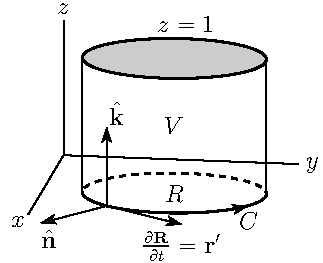
\includegraphics{greens3.pdf}
\end{center}
\end{nfig}
We can now compute the surface integral directly.
\begin{align*}
\dblInt_{\partial V} \vG\cdot\hn\,\dee{S}
&=\dblInt_{\text{side}} \vG\cdot\hn\,\dee{S}  \\
&=\int_a^b\dee{t}\int_0^1\dee{z}\ \vG\big(\vR(t,z)\big)\cdot 
          \big(-x'(t)\,\hj +y'(t)\,\hi\big)
\\
&=\int_a^b\dee{t}\int_0^1\dee{z}\ 
         \big(F_2(x(t),y(t))\,\hi -F_1(x(t),y(t))\,\hj\big)\cdot 
          \big(-x'(t)\,\hj +y'(t)\,\hi\big) \\
&=\int_a^b\dee{t}\ 
         \big[F_2(x(t),y(t))\,y'(t) +F_1(x(t),y(t))\,x'(t)\big]
\\
&\hskip2in \text{since the integrand is independent of $z$}
\\
&=\oint_{C} \big[F_1(x,y)\,\dee{x} +F_2(x,y)\,\dee{y}\big]
\end{align*}
This is exactly the left 
hand side of Green's theorem.
\end{proof}


\begin{eg}\label{eg:greenA}
\noindent\textit{Problem}:
Evaluate
\begin{equation*}
\oint_C\big[(x-xy)\,\dee{x} + (y^3+1)\,\dee{y}
\end{equation*}
where $C$ is the curve given in the figure
\begin{nfig}
\begin{center}
   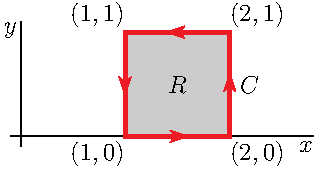
\includegraphics{greensSquare.pdf}
\end{center}
\end{nfig}
\medskip
\noindent\textit{Solution}. Let $R=\Set{(x,y)}{1\le x\le 2,\ 0\le y\le 1}$.
By Green's theorem
\begin{align*}
\oint_C\big[(x-xy)\,\dee{x} + (y^3+1)\,\dee{y}
&=\dblInt_R\Big[\frac{\partial\hfill}{\partial x}(y^3+1) 
                - \frac{\partial\hfill}{\partial y}(x-xy)\Big]\dee{x}\dee{y}\\
&=\int_1^2\dee{x}\int_0^1\dee{y}\ x
=\frac{x^2}{2}\bigg|_1^2
=\frac{3}{2}
\end{align*}
\end{eg}

Here is a simple corollary of Green's theorem that tells how to compute the area enclosed by a curve in the $xy$-plane.
\begin{cor}\label{cor:greens}
Let 
\begin{itemize}\itemsep1pt \parskip0pt \parsep0pt %\itemindent-15pt
\item
$R$ be a finite region in the $xy$-plane whose boundary
\item
$C$ consists of a finite number of piecewise smooth, simple closed curves.
\item
Orient $C$ (i.e. put arrows on $C$) so that if you walk along
$C$ in the direction of the arrows, then $R$ is on your left.

\end{itemize}
Then
\begin{equation*}
\text{Area}(R)
 =\oint_C x\dee{y}
 =-\oint_C y\dee{x}
 =\frac{1}{2}\oint_C \big[x\dee{y} -y\dee{x}\big]
\end{equation*}
\end{cor}
\begin{proof}
This is just Green's theorem applied first with 
$\vF = x\,\hj$, then with $\vF= -y\,\hi$ and finally with 
$\vF = \frac{1}{2}\big[-y\,\hi +x\,\hj\big]$. For all three of these
$\vF$'s,
\begin{equation*}
\frac{\partial F_2}{\partial x} 
                - \frac{\partial F_1}{\partial y} = 1
\end{equation*}
so that Green's theorem gives
\begin{equation*}
\oint_{C} \big[F_1(x,y)\,\dee{x} +F_2(x,y)\,\dee{y}\big]
 =\dblInt_{R}\Big(\frac{\partial F_2}{\partial x} 
                - \frac{\partial F_1}{\partial y}\Big)\ \dee{x}\dee{y}
 =\dblInt_{R}\ \dee{x}\dee{y}
 = \text{Area}(R)
\end{equation*}

\end{proof}


\begin{eg}\label{eg:greenB}
In this example we will use Green's theorem to compute the area enclosed
by the astroid $x^{2/3} + y^{2/3} = a^{2/3}$.
\begin{nfig}
\begin{center}
    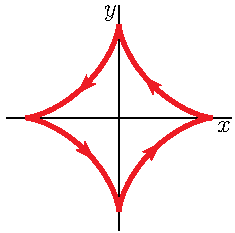
\includegraphics{astroid6.pdf}
\end{center}
\end{nfig}
In Example \ref{eg:astroid} we found the parametrization
\begin{equation*}
\vr(t) = x(t)\,\hi + y(t)\,\hj = a\cos^3t\,\hi + a\sin^3 t\,\hj
\qquad 0\le t\le 2\pi
\end{equation*}
for the astroid. So, by Corollary \ref{cor:greens},
\begin{align*}
\text{Area}
&=\frac{1}{2}\oint_C \big[x\dee{y} -y\dee{x}\big]
 =\frac{1}{2}\int_0^{2\pi} \big[x(t)y'(t) -y(t)x'(t)\big]\dee{t} \\
&=\frac{3a^2}{2}\int_0^{2\pi} \big[\cos^3t\sin^2t\cos t 
                                 +\sin^3t\cos^2 t\sin t\big]\dee{t} \\
&=\frac{3a^2}{2}\int_0^{2\pi} \cos^2t\sin^2t\big[\cos^2t 
                                 +\sin^2t\big]\dee{t} \\
&=\frac{3a^2}{2}\int_0^{2\pi} \cos^2t\sin^2t\ \dee{t} \\
&=\frac{3a^2}{8}\int_0^{2\pi} \sin^2(2t)\ \dee{t} 
=\frac{3a^2}{16}\int_0^{2\pi} [1-\cos(4t)]\ \dee{t} \\
&=\frac{3}{8}a^2\pi
\end{align*}
\end{eg}

\begin{eg}[Trick Question]\label{eg:greenC}
\noindent\textit{Problem}:
Evaluate
\begin{equation*}
\oint_C\vB\cdot\dee{\vr}
\end{equation*}
where
\begin{equation*}
\vB = \frac{-y\,\hi+x\,\hj}{x^2+y^2}
\end{equation*}
and $C$ is the curve
\begin{align*}
x(t) &= \sin(\cos t) \\
y(t) &= \sin(\sin t) \\
z(t) &= 0
\end{align*}
with $0\le t\le 2\pi$.

\medskip
\noindent\textit{Solution}.
First let's think about the curve $C$. If the curve were just
$X(t)=\cos t$, $Y(t)=\sin t$, $Z(t)=0$, it would be the unit circle
centred on the origin in the $xy$-plane, traversed counterclockwise.
For $-\frac{\pi}{2}\le u\le \frac{\pi}{2}$, the function $\sin u$ 
increases monotonically with  $u$ and is of the same sign as $u$ so that,  
since $|\sin t|,|\cos t|\le 1<\frac{\pi}{2}$,
\begin{itemize}\itemsep1pt \parskip0pt \parsep0pt %\itemindent-15pt
\item[$\circ$]
$x(t) = \sin\big(\cos t)$ has the same sign as $X(t)=\cos t$ and is increasing
at precisely the same $t$'s as is $X(t)$
\item[$\circ$]
$y(t) = \sin\big(\sin t)$ has the same sign as $Y(t)=\sin t$ and is increasing
at precisely the same $t$'s as is $Y(t)$
\end{itemize}
So the extra sine in our 
parametrization of $C$ just distorts the circle, straightening the sides a little
as depicted here.
\begin{nfig}
\begin{center}
    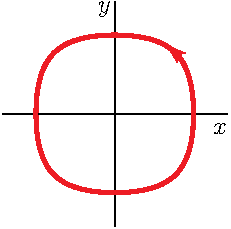
\includegraphics{dcircleA.pdf}
\end{center}
\end{nfig}
It looks like our problem is a straightforward Green's theorem problem
like Example~\ref{eg:greenA}. Let's just try using the strategy of 
Example \ref{eg:greenA}. Because
\begin{align*}
\frac{\partial \vB_2}{\partial x} - \frac{\partial \vB_1}{\partial y}
&=\frac{\partial\hfill}{\partial x}\frac{x}{x^2+y^2} 
                - \frac{\partial\hfill}{\partial y}\frac{-y}{x^2+y^2} \\
&= \frac{1}{x^2+y^2} - \frac{2x^2}{{(x^2+y^2)}^2}
  +\frac{1}{x^2+y^2} - \frac{2y^2}{{(x^2+y^2)}^2}  \\
&= \frac{(x^2+y^2) - 2x^2 + (x^2+y^2) - 2y^2}{{(x^2+y^2)}^2}  \\
&=0
\end{align*}
it looks like Green's theorem gives us, trivially,
\begin{equation*}
\oint_C\vB\cdot\dee{\vr}
=\oint_C\big[\vB_1\,\dee{x} +\vB_2\,\dee{y}\big]
= \dblInt_{R}\left(\frac{\partial B_2}{\partial x} 
                - \frac{\partial B_1}{\partial y}\right)\ \dee{x}\dee{y}
=0
\end{equation*}
where $R$ is the region inside our curve $C$. 

That was easy --- but it's also very \textbf{wrong}!
Our next steps are to 
\begin{itemize}\itemsep1pt \parskip0pt \parsep0pt %\itemindent-15pt
\item
verify that $\oint_C\vB\cdot\dee{\vr}\ne 0$, and 
\item
explain why we got the wrong answer, and
\item
modify our computation so as to give the correct answer.
We'll do this in Example \ref{eg:greenCC}.
\end{itemize}

\noindent
\emph{Verification that $\oint_C\vB\cdot\dee{\vr}\ne 0$:}\ \ \ 

\noindent
Since 
\begin{align*}
x'(t) &= -\cos(\cos t)\ \sin t \\
y'(t) &= \cos(\sin t)\ \cos t \\
z'(t) &= 0
\end{align*}
our integral is
\begin{align*}
\oint_C\vB\cdot\dee{\vr}
&=\oint_C\big[\vB_1\,\dee{x} +\vB_2\,\dee{y}\big]
=\int_0^{2\pi}\big[\vB_1\big(x(t),y(t)\big)\,x'(t) 
            +\vB_2\,\big(x(t),y(t)\big)\,y'(t)\big]\dee{t}
\\
&=\int_0^{2\pi}
            \frac{\sin(\sin t)\,\cos(\cos t)\,\sin t
                  +\sin(\cos t)\,\cos(\sin t)\,\cos t}
                  {\sin^2(\cos t) +\sin^2(\sin t)}
            \dee{t}
\end{align*}
This is a very ugly looking integral\footnote{Indeed!}. 
But even if we can't evaluate the 
integral, we can see that the integrand is strictly positive,
and that forces $\oint_C\vB\cdot\vr>0$. Because
\begin{equation*}
0\le|\sin t|,|\cos t|\le 1<\frac{\pi}{2}
\end{equation*}
\begin{itemize}\itemsep1pt \parskip0pt \parsep0pt %\itemindent-15p
\item[$\circ$]
$\cos(\cos t)>0$, and $\sin(\sin t)$ has the same sign as $\sin t$,
and $\sin(\sin t)$ is zero if and only if $\sin t=0$. 
So the first term in the numerator,
\begin{equation*}
\cos(\cos t)\,\sin(\sin t)\,\sin t\ge 0
\end{equation*} 
and is zero if and only if $\sin t=0$ 
\item[$\circ$]
$\cos(\sin t)>0$, and $\sin(\cos t)$ has the same sign as $\cos t$, and 
$\sin(\cos t)$ is zero if and only if $\cos t=0$. So the second term 
in the numerator,
\begin{equation*}
\cos(\sin t)\,\sin(\cos t)\,\cos t\ge 0
\end{equation*}
and is zero
if and only if $\cos t=0$. 
\item[$\circ$]
There is no $t$ for which both $\sin t$ and $\cos t$ are simultaneously
zero. So the whole numerator 
\begin{equation*}
\sin(\sin t)\,\cos(\cos t)\,\sin t
                  +\sin(\cos t)\,\cos(\sin t)\,\cos t>0
\end{equation*}
is strictly positive.
\end{itemize}
Since the integrand is strictly positive, the integral is strictly positive.

\medskip
\noindent
\emph{Why we got the wrong answer:}

\noindent
In our initial and wrong calculation above, we assumed that 
$\frac{\partial B_2}{\partial x}(x,y) 
                - \frac{\partial B_1}{\partial y}(x,y)=0$
at all points $(x,y)$ of the region $R$ inside $C$. That's not true.
While it is true for most points, it is not true for  \emph{all} points.
The vector field $\vB(x,y)$ is not defined at $(x,y)=(0,0)$.
So $\frac{\partial B_2}{\partial x}(x,y) 
                - \frac{\partial B_1}{\partial y}(x,y)$
is also not defined at $(x,y)=(0,0)$. That's enough to invalidate
Green's theorem. Read the statement of Theorem \ref{thm:Green} again carefully.

\end{eg}

\begin{eg}[Example \ref{eg:greenC}, again.]\label{eg:greenCC}
\noindent\textit{Problem}:
Evaluate
\begin{equation*}
\oint_C\vB\cdot\dee{\vr}
\end{equation*}
where
\begin{equation*}
\vB = \frac{-y\,\hi+x\,\hj}{x^2+y^2}
\end{equation*}
and $C$ is the curve
\begin{align*}
x(t) &= \sin(\cos t) \\
y(t) &= \sin(\sin t) \\
z(t) &= 0
\end{align*}
with $0\le t\le 2\pi$.

\medskip
\noindent\textit{Solution}.
This is the same integral that we computed incorrectly in Example
 \ref{eg:greenC}.
We'll use two ingredients to compute $\oint_C\vB\cdot\dee{\vr}$
correctly.

\begin{itemize}\itemsep1pt \parskip0pt \parsep0pt %\itemindent-15p
\item
Let $a>0$ and denote by $C_a$ the clockwise oriented circle in 
the $xy$-plane that is of radius $a$ and is centered on the origin. 
We can explicitly compute
$\oint_{C_a}\vB\cdot\dee{\vr}$. To do so just parametrize 
$C_a$ by $x(t)=a\cos t$, $y(t) = a\sin t$, $z(t)=0$. Then
$x'(t)=-a\sin t$, $y'(t) = a\cos t$ and
\begin{align*}
\oint_{C_a}\vB\cdot\dee{\vr}
%&=\oint_{C_a}\big[\vB_1\,\dee{x} +\vB_2\,\dee{y}\big]
%=\int_0^{2\pi}\big[\vB_1\big(x(t),y(t)\big)\,x'(t) 
%            +\vB_2\,\big(x(t),y(t)\big)\,y'(t)\big]\dee{t}
%\\
&=\int_0^{2\pi}\Big[\frac{-a\sin t\,\hi+a\cos t\,\hj}
                            {a^2\cos^2t+a^2\sin^2t}\Big]
           \cdot\big[-a\sin t\,\hi+a\cos t\,\hj\big]
           \dee{t}
=\int_0^{2\pi}\dee{t}=2\pi
\end{align*}

\item
Pick an $a$ that is small enough that $C_a$ lies entirely inside $C$ and
apply Green's theorem with the region, $R_a$, that is between $C$ and $C_a$.
\vadjust{ 
\begin{nfig}
\begin{center}
    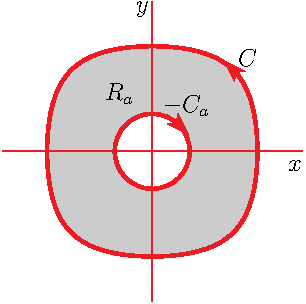
\includegraphics{dcircleB.pdf}
\end{center}
\end{nfig}
}
The curve bounding $R_a$ has two components --- $C$ and $C_a$, but now $C_a$
is oriented clockwise. (Recall that, in Green's theorem, when you walk along a boundary curve in the direction of the arrow, $R_a$ has to be on your left.). Use 
$-C_a$ to denote $C_a$ oriented clockwise. 
$\frac{\partial B_2}{\partial x}(x,y) 
                - \frac{\partial B_1}{\partial y}(x,y)$ really is zero
at \emph{all} points $(x,y)$ of the region $R_a$. So Green's theorem gives
\begin{align*}
0&= \dblInt_{R_a}\Big(\frac{\partial B_2}{\partial x} 
                - \frac{\partial B_1}{\partial y}\Big)\ \dee{x}\dee{y} 
  = \oint_{C}\vB\cdot\dee{\vr} + \oint_{-C_a}\vB\cdot\dee{\vr} \\
 & = \oint_{C}\vB\cdot\dee{\vr} - \oint_{C_a}\vB\cdot\dee{\vr} 
\end{align*}
and so
\begin{align*}
\oint_{C}\vB\cdot\dee{\vr}
= \oint_{C_a}\vB\cdot\dee{\vr}
=2\pi
\end{align*}
\end{itemize}

\intremark{
\noindent
\emph{Why Green's theorem applies to $R_a$:}

\begin{itemize}\itemsep1pt \parskip0pt \parsep0pt %\itemindent-15p
\item[$\circ$]
Remove from $R_a$ a narrow path joining the central hole and the outside world
as in the figure

\begin{center}
    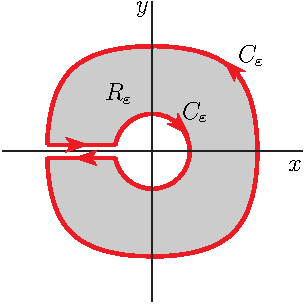
\includegraphics{dcircleC.pdf}
\end{center}

\noindent Call the resulting region $R_\veps$, when the path has width $\veps$,
and denote by $C_\veps$ the bounding curve of $R_\veps$.
Theorem \ref{thm:Green} does apply to $R_\veps$, so
\begin{align*}
\oint_{C_\veps}\vB\cdot\dee{\vr}
=\dblInt_{R_\veps}\Big(\frac{\partial B_2}{\partial x} 
                - \frac{\partial B_1}{\partial y}\Big)\ \dee{x}\dee{y} 
=0
\end{align*}

\item[$\circ$] Now take the limit $\veps\rightarrow 0$. This gives 
\begin{align*}
\oint_{C_0}\vB\cdot\dee{\vr}
=\lim_{\veps\rightarrow 0}\oint_{C_\veps}\vB\cdot\dee{\vr}
%=\lim_{\veps\rightarrow 0}\dblInt_{R_\veps}\Big(\frac{\partial B_2}{\partial x} 
%                - \frac{\partial B_1}{\partial y}\Big)\ \dee{x}\dee{y} 
%=\dblInt_{R_a}\Big(\frac{\partial B_2}{\partial x} 
%                - \frac{\partial B_1}{\partial y}\Big)\ \dee{x}\dee{y} 
=0
\end{align*}
where $C_0$ is the curve in the figure

\begin{center}
    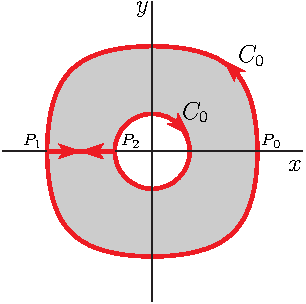
\includegraphics{dcircleD.pdf}
\end{center}

\noindent
Pick any point $P_0$ on the original curve $C$. The curve $C_0$
\begin{itemize}\itemsep1pt \parskip0pt \parsep0pt %\itemindent-15p
\item
first\footnote{It doesn't matter where $C_0$ starts from.
For concreteness, we can start it at the point, $P_0=(\sin 1,0,0)$, where 
the original curve $C$ intersects the positive $x$-axis.} 
follows the original curve $C$ from $P_0$ counterclockwise to the point $P_1$
on the negative $x$-axis.
\item 
Then it follows the negative $x$-axis towards the origin until it
hits $C_a$ at the point $P_2$.
\item 
Then it circumnavigates $C_a$ once clockwise, returning to $P_2$.
\item
Then it follows the negative $x$-axis away from the origin until it
returns to $P_1$.
\item
Finally it follows $C$ back to its starting point.
\end{itemize}

\item[$\circ$]
So
\begin{align*}
0=\oint_{C_0}\vB\cdot\dee{\vr}
&=\oint_{C}\vB\cdot\dee{\vr}
 +\oint_{\overline{P_1 P_2}}\vB\cdot\dee{\vr}
 +\oint_{-C_a}\vB\cdot\dee{\vr}
 +\oint_{\overline{P_2 P_1}}\vB\cdot\dee{\vr} \\
&=\oint_{C}\vB\cdot\dee{\vr}
 +\oint_{\overline{P_1 P_2}}\vB\cdot\dee{\vr}
 +\oint_{-C_a}\vB\cdot\dee{\vr}
 -\oint_{\overline{P_1 P_2}}\vB\cdot\dee{\vr} \\
&=\oint_{C}\vB\cdot\dee{\vr}
 +\oint_{-C_a}\vB\cdot\dee{\vr}
\end{align*}
as desired.
\end{itemize}
}
\end{eg}


%%%%%%%%%%%%%%%%%%%%%%%%%%
\section{Stokes' Theorem}\label{sec:StokesThm}
%%%%%%%%%%%%%%%%%%%%%%%%%
Our last variant of the fundamental theorem of calculus is 
Stokes'\footnote{Sir George Gabriel Stokes (1819--1903) was an Irish physicist and mathematician. In addition to Stokes' theorem, he is known for the Navier-Stokes equations of fluid dynamics and for his work on the wave theory
of light. He gave evidence to the Royal Commission on the Use of Iron in 
Railway Structures after the Dee bridge disaster of 1847.} theorem, which is like Green's theorem, but in three dimensions.
It relates an integral over a finite surface 
in $\bbbr^3$ with an integral over the curve bounding the surface. 

\begin{theorem}[Stokes' Theorem]\label{thm:Stokes}
Let 
\begin{itemize}\itemsep1pt \parskip0pt \parsep0pt %\itemindent-15pt
\item
$S$ be a piecewise smooth oriented surface (i.e. a unit normal $\hn$ has 
been chosen at each point of $S$ and this choice depends continuously
on the point)
\item
the boundary, $\partial S$, of the surface $S$ consist of a finite number of piecewise smooth, simple curves that are oriented consistently with $\hn$ in the sense that
    \begin{itemize}\itemsep1pt \parskip0pt \parsep0pt %\itemindent-15pt
    \item
    if you walk along $\partial S$ in the direction of the arrow
    on $\partial S$,
     \item
     with the vector from your feet to your head  having direction $\hn$
    \item
    then $S$ is on your left hand side.
    \end{itemize}

\begin{center}
    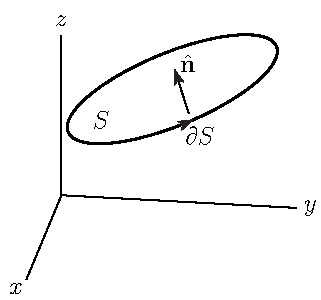
\includegraphics{stokes0.pdf}
\end{center}


\item
$\vF$ be a vector field that has continuous first partial derivatives 
at every point of $S$.
\end{itemize}
Then
\begin{equation*}
\oint_{\partial S}\vF\cdot \dee{\vr}
  =\dblInt_{S}\vnabla\times\vF\cdot\hn\ \dee{S}
\end{equation*}

\end{theorem}
Note that
\begin{itemize}
\item
in Stokes' theorem, $S$ must be an oriented surface. In particular, $S$ may not be a M\"obius strip. (See Example \ref{eg:orientMobius}.)
\item
If $S$ is part of the $xy$-plane, then Stokes' theorem reduces to Green's
theorem. Our proof of Stokes' theorem will consist of rewriting the integrals 
%that appear in Stoke's theorem 
so as to allow an application of Green's theorem.
\item
If $\partial S$ is simple closed curve and
\begin{itemize}
\item
when you look at $\partial S$ from high on the $z$-axis, it is oriented
counterclockwise (look at the figure in Theorem \ref{thm:Stokes}), then
\item 
$\hn$ is upward pointing, i.e. has positive $z$-component, at least near 
$\partial S$.
\end{itemize}
\end{itemize}

\begin{proof}
Write $\vF=F_1\,\hi+F_2\,\hj+F_3\,\hk$.
Both integrals involve $F_1$ terms and $F_2$ terms and
$F_3$ terms. We shall show that the $F_1$ terms in the two integrals agree.
In other words, we shall assume that $\vF=F_1\hi$.
The proofs that the $F_2$ and $F_3$ terms also agree are similar.
For simplicity, we'll assume\footnote{Otherwise, decompose $S$ into simpler pieces, analogously to what we did in the proof of the divergence theorem.} 
that the boundary of $S$ consists of just a single curve, and that we can
\begin{itemize}\itemsep1pt \parskip0pt \parsep0pt %\itemindent15pt
\item[$\circ$]
pick a parametrization of $S$ with
\begin{equation*}
S=\Set{\vr(u,v)=\big(x(u,v),y(u,v),z(u,v)\big)}{ (u,v)\text{ in }
                 R\subset\bbbr^2}
\end{equation*}
and with $\vr(u,v)$ orientation preserving in the sense that
$\hn\,\dee{S} = +\frac{\partial \vr}{\partial u}
\times \frac{\partial \vr}{\partial v}\,\dee{u}\,\dee{v}$. Also
\item[$\circ$] pick a parametrization of the curve, $\partial R$, bounding $R$ as 
$\big( u(t), v(t)\big)$, $a\le t\le b$, in such a way that 
%the velocity vector $\big( u'(t), v'(t)\big)$ is never zero, and 
when you walk along $\partial R$ in the direction of increasing $t$, then $R$ 
is on your left. 
\end{itemize}
Then the curve $\partial S$ bounding $S$ 
can be parametrized as $\vR(t)=\vr\big(u(t),v(t)\big)$, $a\le t\le b$.
\vadjust{
\begin{efig}
\begin{center}
    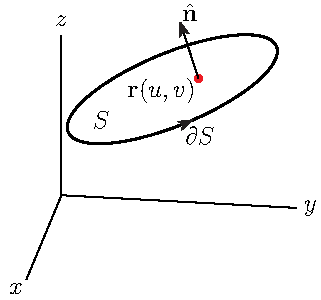
\includegraphics{stokes1.pdf}\qquad\qquad
    \raisebox{15pt}{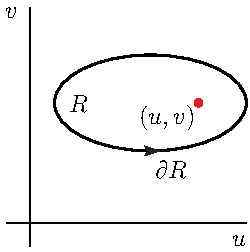
\includegraphics{stokes2.pdf}}
\end{center}
\end{efig}
}

\noindent
\emph{The orientation of $\vR(t)$:}\ \ \

We'll now verify that the direction of increasing $t$ for the parametrization 
$\vR(t)$ of $\partial S$ is the direction of the arrow on $\partial S$ 
in the figure on the left above.
%For simplicity, suppose that $\partial R$ is connected. 
By continuity, it suffices to check the orientation at a single point.

Find a point $(u_0,v_0)$ on $\partial R$ where the forward pointing 
tangent vector is a positive multiple of $\,\hi$. The horizontal 
arrow on $\partial R$ 
in the figure on the left below is at such a point. Suppose that 
$t=t_0$ at this point --- in other words, suppose 
that $(u_0,v_0)=\big(u(t_0),v(t_0)\big)$. 
Because  the forward pointing tangent vector to $\partial R$ at 
$(u_0,v_0)$, namely $\big(u'(t_0),v'(t_0)\big)$,
 is a positive multiple of $\,\hi$, we have $u'(t_0)>0$ and 
$v'(t_0)=0$. 
The tangent vector to $\partial S$ at $ \vR(t_0)=\vr\big(u_0,v_0\big)$,
pointing in the direction of increasing $t$, is 
\begin{align*}
\vR'(t_0)&=\diff{\hfill}{t}\vr\big(u(t),v(t)\big)\big|_{t=t_0}
=u'(t_0)\frac{\partial \vr}{\partial u}(u_0,v_0)
+v'(t_0) \frac{\partial \vr}{\partial v}(u_0,v_0) \\
&=u'(t_0)\frac{\partial \vr}{\partial u}(u_0,v_0)
\end{align*}
and so is a positive multiple of $\frac{\partial \vr}{\partial u}(u_0,v_0)$.
See the figure on the right below.
 
If we now walk along a path in the $uv$-plane which starts at $(u_0,v_0)$,
holds $u$ fixed at $u_0$ and increases $v$, we move into the interior of 
$R$ starting at $(u_0,v_0)$. Correspondingly, if we walk along the path,
$\vr(u_0,v)$, in $\bbbr^3$ with $v$ starting at $v_0$ and increasing,
we move into the interior of $S$. The forward tangent to this new path, 
$\frac{\partial \vr}{\partial v}(u_0,v_0)$,
points from $ \vr(u_0,v_0)$ into the interior of $S$. It's the blue arrow in
the figure on the right below.

\begin{wfig}
\begin{center}
    \raisebox{20pt}{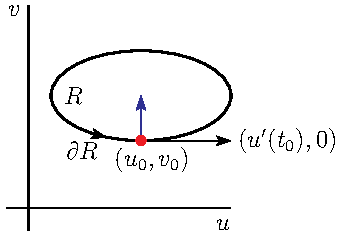
\includegraphics{stokes4.pdf}}
    \raisebox{100pt}{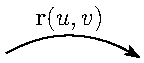
\includegraphics{stokes5.pdf}}
    \includegraphics{stokes3.pdf}
\end{center}
\end{wfig}


Now imagine that you are walking along $\partial S$ in the direction of
increasing $t$. At time $t_0$ you are at $\vR(t_0)$. You point your right arm
straight ahead of you. So it is pointing in the direction
$\frac{\partial \vr}{\partial u}(u_0,v_0)$. You point your left arm
out sideways into the interior of $S$. It is pointing in the 
direction $\frac{\partial \vr}{\partial v}(u_0,v_0)$. If the direction
of increasing $t$ is the same as the forward direction of the orientation
of $\partial S$, then the vector from our feet to our head, which is 
$\frac{\partial \vr}{\partial u}(u_0,v_0)
\times \frac{\partial \vr}{\partial v}(u_0,v_0)$, should be pointing in
the same direction as $\hn$. And since 
$\hn\,\dee{S} = +\frac{\partial \vr}{\partial u}
     \times \frac{\partial \vr}{\partial v}\,\dee{u}\,\dee{v}$, it is.

Now, with our parametrization and orientation sorted out, we can examine
the integrals.

\bigskip
\noindent
\emph{The surface integral:}\ \ \

Since $F=F_1\,\hi$, so that 
\begin{align*}
\vnabla\times\vF
&=\det\left[\begin{matrix} \hi & \hj & \hk \\[0.05in]
         \frac{\partial\hfill}{\partial x} & \frac{\partial\hfill}{\partial y} &
                         \frac{\partial\hfill}{\partial z} \\[0.05in]
         F_1 & 0 & 0
       \end{matrix}\right] 
= \left(0,\frac{\partial F_1}{\partial z}, 
                -\frac{\partial F_1}{\partial y}\right)
\end{align*}
and 
\begin{align*}
\hn\,\dee{S}
&=\frac{\partial \vr}{\partial u} \times \frac{\partial \vr}{\partial v}
         \ \dee{u}\,\dee{v} 
=\det\left[\begin{matrix} \hi & \hj & \hk \\
         \frac{\partial x}{\partial u} & \frac{\partial y}{\partial u} &
                         \frac{\partial z}{\partial u} \\[0.05in]
         \frac{\partial x}{\partial v} & \frac{\partial y}{\partial v} &
                         \frac{\partial z}{\partial v}
       \end{matrix}\right] \\
&=\left(\frac{\partial y}{\partial u}
                         \frac{\partial z}{\partial v}
                       -\frac{\partial z}{\partial u}
                       \frac{\partial y}{\partial v}\right)\hi
  + \left(\frac{\partial z}{\partial u}
                         \frac{\partial x}{\partial v}
                       -\frac{\partial x}{\partial u}
                       \frac{\partial z}{\partial v}\right)\hj
  +\left(\frac{\partial x}{\partial u}
                         \frac{\partial y}{\partial v}
                       -\frac{\partial y}{\partial u}
                       \frac{\partial x}{\partial v}\right) \hk
\end{align*}
and
\begin{align*}
&\dblInt_{S}\vnabla\times\vF\cdot\hn\,\dee{S}
=\dblInt_{R}\left(0,\frac{\partial F_1}{\partial z}, 
                -\frac{\partial F_1}{\partial y}\right)
   \cdot\frac{\partial \vr}{\partial u}
\times \frac{\partial \vr}{\partial v}\ \dee{u}\,\dee{v}\cr
&\hskip.15in=\dblInt_{R}\left\{\frac{\partial F_1}{\partial z}
                    \left(\frac{\partial z}{\partial u}
                         \frac{\partial x}{\partial v}
                       -\frac{\partial x}{\partial u}
                       \frac{\partial z}{\partial v}\right)
-\frac{\partial F_1}{\partial y}
                    \left(\frac{\partial x}{\partial u}
                         \frac{\partial y}{\partial v}
                       -\frac{\partial y}{\partial u}
                       \frac{\partial x}{\partial v}\right)
\right\}\,\dee{u}\,\dee{v}
\end{align*}
Now we examine the line integral and show that it equals this one.

\bigskip
\noindent
\emph{The line integral:}\ \ \ 
\begin{align*}
\oint_{\partial S}\vF\cdot \dee{\vr}
&=\int_a^b\vF\Big(\vr\big(u(t),v(t)\big)\Big)\cdot\diff{\hfill}{t}
\vr\big(u(t),v(t)\big)\ \dee{t} \\
&=\int_a^b\vF\Big(\vr\big(u(t),v(t)\big)\Big)\cdot\Big[
\frac{\partial\vr}{\partial u}\big(u(t),v(t)\big)\diff{u}{t}(t)
+\frac{\partial\vr}{\partial v}\big(u(t),v(t)\big)\diff{v}{t}(t)\Big]\ \dee{t}
\end{align*}
We can write this as the line integral
\begin{equation*}
\oint_{\partial R}M(u,v)\ \dee{u}+N(u,v)\ \dee{v}
=\int_a^b \Big[M\big(u(t),v(t)\big)\ \diff{u}{t}(t)
+N\big(u(t),v(t))\ \diff{v}{t}(t)\Big]\ \dee{t}
\end{equation*}
around $\partial R$, if we choose
\begin{alignat*}{3}
M(u,v)&=\vF\big(\vr(u,v)\big)\cdot\frac{\partial\vr}{\partial u}(u,v)
&&=F_1\big({x(u,v),y(u,v),z(u,v)}\big)\frac{\partial x}{\partial u}(u,v)\\
N(u,v)&=\vF\big(\vr(u,v)\big)\cdot\frac{\partial\vr}{\partial v}(u,v)
&&=F_1\big({x(u,v),y(u,v),z(u,v)}\big)\frac{\partial x}{\partial v}(u,v)
\end{alignat*}

\bigskip
\noindent
\emph{Finally, we show that the surface integral equals the line integral:}\ \ \

By Green's Theorem, we have
\begin{align*}
\oint_{\partial S}\vF\cdot \dee{\vr}
&=\oint_{\partial R}M(u,v)\ \dee{u}+N(u,v)\ \dee{v}\cr
=\dblInt_{R}\bigg\{&\frac{\partial N}{\partial u}-\frac{\partial M}{\partial v}
\bigg\}\ \dee{u} \dee{v}\cr
=\dblInt_{R}\bigg\{&
               \frac{\partial\hfill}{\partial u}\big[
                     F_1\big({x(u,v),y(u,v),z(u,v)}\big)
                     \big]\frac{\partial x}{\partial v}
                   +F_1\frac{\partial^2 x}{\partial u\partial v} \\
-& \frac{\partial\hfill}{\partial v}\big[
                     F_1\big({x(u,v),y(u,v),z(u,v)}\big)
                     \big]\frac{\partial x}{\partial u}
                   -F_1\frac{\partial^2 x}{\partial v\partial u}
                                        \bigg\}\ \dee{u} \dee{v}
\displaybreak[0]\\
=\dblInt_{R}\bigg\{&
               \textcolor{blue}{\Big(\frac{\partial F_1}{\partial x}
                     \frac{\partial x}{\partial u}}
                     +\frac{\partial F_1}{\partial y}
                     \frac{\partial y}{\partial u}
                     +\frac{\partial F_1}{\partial z}
                     \frac{\partial z}{\partial u}
                     \Big)\frac{\partial x}{\partial v}
                \textcolor{red}{
                   +F_1\frac{\partial^2 x}{\partial u\partial v}}\cr
-&\Big(
              \textcolor{blue}{\frac{\partial F_1}{\partial x}
                     \frac{\partial x}{\partial v}}
                     +\frac{\partial F_1}{\partial y}
                     \frac{\partial y}{\partial v}
                     +\frac{\partial F_1}{\partial z}
                     \frac{\partial z}{\partial v}
                     \Big)\frac{\partial x}{\partial u}
                \textcolor{red}{
                   -F_1\frac{\partial^2 x}{\partial v\partial u}}
                                        \bigg\}\ \dee{u} \dee{v}\cr
=\dblInt_{R}\bigg\{&\Big(\frac{\partial F_1}{\partial y}
                     \frac{\partial y}{\partial u}
                     +\frac{\partial F_1}{\partial z}
                     \frac{\partial z}{\partial u}
                     \Big)\frac{\partial x}{\partial v}
%\cr-&
-\Big(\frac{\partial F_1}{\partial y}
                     \frac{\partial y}{\partial v}
                     +\frac{\partial F_1}{\partial z}
                     \frac{\partial z}{\partial v}
                     \Big)\frac{\partial x}{\partial u}
\bigg\}\,\dee{u}\, \dee{v}\cr
\noalign{\vskip.05in}
&\hskip-33pt=\dblInt_{S}\vnabla\times\vF\cdot\hn\,\dee{S}
\end{align*}
which is the conclusion that we wanted.
\end{proof}

Before we move on to some examples, here are a couple of remarks.

\begin{itemize}
\item
Stokes' theorem says that 
$\oint_{C}\vF\cdot \dee{\vr}
  =\dblInt_{S}\vnabla\times\vF\cdot\hn\ \dee{S}$
for any (suitably oriented) surface whose boundary is $C$. So if
$S_1$ and $S_2$ are two different (suitably oriented) surfaces having the 
same boundary curve $C$, then
\begin{equation*}
\dblInt_{S_1}\vnabla\times\vF\cdot\hn\ \dee{S}
=\dblInt_{S_2}\vnabla\times\vF\cdot\hn\ \dee{S}
\end{equation*}
For example, if $C$ is the unit circle
\begin{equation*}
C=\Set{(x,y,z)}{x^2+y^2=1,\ z=0}
\end{equation*}
oriented counterclockwise when viewed from above, then both
\begin{align*}
S_1&= \Set{(x,y,z)}{x^2+y^2\le 1,\ z=0} \\
S_2&= \Set{(x,y,z)}{z\ge0,\ x^2+y^2+z^2=1} 
\end{align*}
with upward pointing unit normal vectors, have boundary $C$. So Stokes'
tells us that $\dblInt_{S_1}\vnabla\times\vF\cdot\hn\ \dee{S}
=\dblInt_{S_2}\vnabla\times\vF\cdot\hn\ \dee{S}$.
\begin{nfig}
\begin{center}
    \includegraphics{twoSurfaceA.pdf}
\end{center}
\end{nfig}
It should not be a surprise that $\dblInt_{S_1}\vnabla\times\vF\cdot\hn\ \dee{S}
=\dblInt_{S_2}\vnabla\times\vF\cdot\hn\ \dee{S}$, for the following reason.
Let 
\begin{equation*}
V= \Set{(x,y,z)}{x^2+y^2+z^2\le 1,\ z\ge 0} \\
\end{equation*}
be the solid between $S_1$ and $S_2$.
The boundary $\partial V$ of $V$ is the union of $S_1$ and $S_2$.
\vadjust{
\begin{nfig}
\begin{center}
    \includegraphics{twoSurfaceB.pdf}
\end{center}
\end{nfig}
}
But beware that the outward pointing normal to $\partial V$ (call it
$\hN$) is $+\hn$ on $S_2$ and $-\hn$ on $S_1$. So the divergence 
theorem gives
\begin{align*}
\dblInt_{S_2}\vnabla\times\vF\cdot\hn\ \dee{S}
-\dblInt_{S_1}\vnabla\times\vF\cdot\hn\ \dee{S}
&= \dblInt_{S_2}\vnabla\times\vF\cdot\hN\ \dee{S}
+\dblInt_{S_1}\vnabla\times\vF\cdot\hN\ \dee{S} \\
&= \dblInt_{\partial V}\vnabla\times\vF\cdot\hN\ \dee{S} \\
&= \tripInt_{V}\vnabla\cdot\big(\vnabla\times\vF\big)\ \dee{V} \\[-0.2in]
&\hskip1in\qquad\text{by the divergence theorem} \\
&=0
\end{align*}
by the vector identity Theorem \ref{thm:degTwoIdentities}.a.





\item
As a second remark, suppose that the vector field $\vF$ obeys $\vnabla\times\vF=\vZero$ everywhere. Then Stokes' theorem forces
$\oint_{C}\vF\cdot \dee{\vr}=0$ are around all closed curves $C$,
which implies that $\vF$ is conservative, by 
Theorem \ref{thm:pathIndepConserv}. So Stokes' theorem provides
another proof of Theorem \ref{thm:screenConserv}.

\end{itemize}

Here is an easy example which shows that Stokes' can be very useful 
when $\vnabla\times\vF$ simplifies.


\begin{eg}\label{eg:stokesAA}
\noindent\textit{Problem}:
Evaluate
$
\oint_C\vF\cdot\dee{\vr}
$
where $\vF= \big[2z+\sin\big(x^{146}\big)\big]\,\hi-5z\,\hj -5y\,\hk$ 
and the curve $C$ is the circle $x^2+y^2=4$, $z=1$, 
oriented counterclockwise when viewed from above.

\medskip
\noindent\textit{Solution}. 
The $x^{146}$ in $\vF$ will probably make a direct evaluation of the
integral difficult. So we'll use Stokes' theorem. To do so we need
a surface $S$ with $\partial S=C$. The simplest is just the flat
disk
\begin{equation*}
S = \Set{(x,y,z)}{ x^2+y^2\le 4,\ \ z=1}
\end{equation*}
\begin{nfig}
\begin{center}
    \includegraphics{horizontalDiskB.pdf}
\end{center}
\end{nfig}
Since
\begin{align*}
\vnabla\times\vF & = \det\left[\begin{matrix}
                         \hi & \hj & \hk \\[0.05in]
                         \frac{\partial\hfill}{\partial x} &
                         \frac{\partial\hfill}{\partial y} &
                         \frac{\partial\hfill}{\partial z} \\
                              2z+\sin\big(x^{146}\big)  &  -5z  & -5y
                               \end{matrix}\right] \\
& =\hi \det\left[\begin{matrix}
                         \frac{\partial\hfill}{\partial y} &
                         \frac{\partial\hfill}{\partial z} \\
                               -5z  & -5y
                               \end{matrix}\right] 
   -\hj\det\left[\begin{matrix}
                         \frac{\partial\hfill}{\partial x} &
                         \frac{\partial\hfill}{\partial z} \\
                              2z+\sin\big(x^{146}\big)   & -5y
                               \end{matrix}\right] 
   +\hk\det\left[\begin{matrix}
                         \frac{\partial\hfill}{\partial x} &
                         \frac{\partial\hfill}{\partial y}  \\
                              2z+\sin\big(x^{146}\big)  &  -5z  
                               \end{matrix}\right]\\
  &=2\hj
\end{align*}
and the normal to $S$ is $\hk$,
Stokes' theorem gives
\begin{align*}
\oint_C\vF\cdot\dee{\vr}
& = \dblInt_S \vnabla\times\vF\cdot\hn\,\dee{S}
=  \dblInt_S (2\hj)\cdot\hk\,\dee{S}
=0
\end{align*}

\end{eg}

Now we'll repeat the last example with a harder curve.

\begin{eg}\label{eg:stokesA}
\noindent\textit{Problem}:
Evaluate
$
\oint_C\vF\cdot\dee{\vr}
$
where $\vF= \big[2z+\sin\big(x^{146}\big)\big]\,\hi-5z\,\hj -5y\,\hk$ 
and the curve $C$ is the intersection of $x^2+y^2+z^2=4$ 
and $z=y$, oriented counterclockwise when viewed from above.

\medskip
\noindent\textit{Solution}. 
The surface $x^2+y^2+z^2=4$ is the sphere of radius $2$ centred on the origin
and $z=y$ is a plane which contains the origin. So $C$, being the 
intersection of a sphere with a plane through the centre of the sphere,
is a circle, with centre $(0,0,0)$ and radius $2$. The part of the circle
in the first octant is sketched on the left below.
\vadjust{
\begin{nfig}
\begin{center}
    \includegraphics{circle4c.pdf} \qquad\quad
    \includegraphics{circle4d.pdf}
\end{center}
\end{nfig}
}
The $x^{146}$ in $\vF$ will probably make a direct evaluation of the
integral difficult. So we'll use Stokes' theorem. To do so we need
a surface $S$ with $\partial S=C$. The simplest is the flat
disk
\begin{equation*}
S = \Set{(x,y,z)}{ x^2+y^2+z^2\le 4,\ \ z=y}
\end{equation*}
The first octant of $S$ is shown in the figure on the right above.
We saw in the last Example \ref{eg:stokesAA} that
\begin{align*}
\vnabla\times\vF &=2\hj
\end{align*}
So Stokes' theorem gives
\begin{align*}
\oint_C\vF\cdot\dee{\vr}
& = \dblInt_S \vnabla\times\vF\cdot\hn\,\dee{S}
 = 2\dblInt_S \hj\cdot\hn\,\dee{S}
\end{align*}

We'll evaluate the integral $2\dblInt_S \hj\cdot\hn\,\dee{S}$ in two ways.
The first way is more efficient, but also requires more insight.
Since $\vnabla(z-y)=\hk-\hj$, the upward unit normal to the plane $z-y=0$, 
and hence to $S$, is $\hn = \frac{1}{\sqrt{2}}(\hk-\hj)$.
Consequently the integrand 
\begin{align*}
\hj\cdot\hn=\hj\cdot\Big(\frac{-\hj+\hk}{\sqrt{2}}\Big)=-\frac{1}{\sqrt{2}}
\end{align*}
is a constant and we do not need a formula for $\hn\,dS$:
\begin{align*}
\oint_C\vF\cdot\dee{\vr}
& = 2\dblInt_S \hj\cdot\hn\,\dee{S}
=-\sqrt{2} \dblInt_S \dee{S} 
= -\sqrt{2}\text{Area}(S)
=-\sqrt{2}\pi\, 2^2 \\
&=-4\sqrt{2}\pi
\end{align*}

Alternatively, we can evaluate the integral $\dblInt_S \hj\cdot\hn\,\dee{S}$
using our normal protocol. 
As $S$ is part of the plane $z=f(x,y)=y$,
\begin{align*}
\hn\,dS = \pm\big(-f_x\,\hi-f_y\,\hj+\hk\big)\,\dee{x}\dee{y}
        = \pm (-\hj+\hk)\,\dee{x}\dee{y}
\end{align*}
To get the upward pointing normal pointing normal, we take the $+$ sign
so that $\hn\,dS= (-\hj+\hk)\,\dee{x}\dee{y}$. As $(x,y,z)$ runs over
\begin{align*}
S &= \Set{(x,y,z)}{ x^2+y^2+z^2\le 4,\ \ z=y}
  = \Set{(x,y,z)}{ x^2+2y^2\le 4,\ \ z=y} \\
  &= \Set{(x,y,z)}{ \tfrac{x^2}{4} +\tfrac{y^2}{2}\le 1,\ \ z=y} 
\end{align*}
$(x,y)$ runs over the elliptical disk 
$R=\Set{(x,y)}{\frac{x^2}{4} +\frac{y^2}{2}\le 1}$. 
The part of this ellipse in the first octant is the shaded region in 
the figure below.
\vadjust{
\begin{nfig}
\begin{center}
    \includegraphics{circle4e.pdf}
\end{center}
\end{nfig}
}
This ellipse has semiaxes $a=2$ and $b =\sqrt{2}$ and hence area $\pi a b = 2\sqrt{2} \pi$. So
\begin{align*}
\oint_C\vF\cdot\dee{\vr}
& = 2\dblInt_S \hj\cdot\hn\,\dee{S}
=2\dblInt_R \hj\cdot(-\hj+\hk)\,\dee{x}\dee{y}
=-2 \dblInt_R \dee{x}\dee{y} 
= -2\text{Area}(R)\\
&=-4\sqrt{2}\pi
\end{align*}
\end{eg}

\begin{eg}\label{eg:stokesB}
\noindent\textit{Problem}:
Evaluate
$
\oint_C\vF\cdot\dee{\vr}
$
where $\vF= (x+y)\,\hi+2(x-z)\,\hj +(y^2+z)\,\hk$ 
and $C$ is the oriented curve  obtained by 
going from $(2,0,0)$ to $(0, 3, 0)$ to $(0, 0, 6)$ and back to 
$(2, 0, 0)$ along straight line segments. 

\begin{nfig}
\begin{center}
    \includegraphics{domainTriangle.pdf}
\end{center}
\end{nfig}


\medskip
\noindent\textit{Solution 1}. 
In this first solution, we'll evaluate the integral directly.
The first line segment ($C_1$ in the figure above) may be parametrized as
\begin{equation*}
\vr(t)=(2,0,0)+t\big\{(0, 3, 0)-(2,0,0)\big\}
=\big(2-2t\,,\,3t\,,\,0\big)\qquad 0\le t\le 1
\end{equation*} 
So the integral along this segment is
\begin{align*}
\int_0^1 \vF(\vr(t))\cdot\diff{\vr}{t}\ \dee{t}
&=\int_0^1 (2+t\,,\, 2(2-2t)\,,\, (3t)^2)\cdot(-2\,,\, 3\,,\, 0)\ \dee{t}
=\int_0^1 (8-14t)\ \dee{t} \\
&=\Big[8t-7t^2\Big]_0^1=1
\end{align*}
%%%%%
The second line segment ($C_2$ in the figure above) may be parametrized as
\begin{equation*}
\vr(t)=(0,3,0)+t\big\{(0, 0, 6)-(0,3,0)\big\}
=\big(0\,,\,3-3t\,,\,6t\big)\qquad 0\le t\le 1
\end{equation*}. 
So the integral along this segment is
\begin{align*}
\int_0^1 \vF(\vr(t))\cdot\diff{\vr}{t}\ \dee{t}
&=\int_0^1 \big(3(1-t)\,,\, - 12t\,,\, 9(1-t)^2+ 6t\big)\cdot(0, -3, 6)\ \dee{t}
\\
&=\int_0^1 [36t+54(1-t)^2+36t]\ \dee{t}
=\Big[18t^2-18(1-t)^3+18t^2\Big]_0^1
\\
&=54
\end{align*}
The final line segment ($C_3$ in the figure above) may be parametrized as
\begin{equation*}
\vr(t)=(0,0,6)+t\big\{(2,0,0) -(0,0,6)\big\} = (2t\,,\,0\,,\,6-6t)
\qquad 0\le t\le 1
\end{equation*}
So the line integral along this segment is
\begin{align*}
\int_0^1 \vF(\vr(t))\cdot\diff{\vr}{t}\ \dee{t}
&=\int_0^1 \big(2t\,,\, 4t - 12(1-t)\,,\,  6(1-t)\big)\cdot(2, 0, -6)\ \dee{t}
\\
&=\int_0^1 [4t-36(1-t)]\ \dee{t}
=\Big[2t^2+18(1-t)^2\Big]_0^1
=-16
\end{align*}
The full line integral is
\begin{equation*}
\oint_C\vF\cdot \dee{\vr}=1+54-16=39
\end{equation*}


\medskip
\noindent\textit{Solution 2}. 
This time we shall apply Stokes' Theorem. The curl of $\vF$ is
\begin{equation*}
\vnabla\times\vF
=\det\left[\begin{matrix}
          \hi & \hj &\hk \\[0.05in]
          \frac{\partial\hfill}{\partial x} &
              \frac{\partial\hfill}{\partial y} &
              \frac{\partial\hfill}{\partial z}  \\
           x+y & 2(x-z) & y^2+z
          \end{matrix}
     \right] 
=(2y+2)\hi-(0-0)\hj+(2-1)\hk=2(y+1)\hi+\hk
\end{equation*}
The curve $C$ is a triangle and so is contained in a plane.
Any plane has an equation of the form $Ax+By+Cz=D$.
Our plane does not pass through the origin (look at the figure above)
so the $D$ must be nonzero. Consequently we may divide $Ax+By+Cz=D$ through 
by $D$ giving an equation of the form $ax+by+cz=1$. 
\begin{itemize}\itemsep1pt \parskip0pt \parsep0pt %\itemindent-15pt
\item[$\circ$] Because $(2,0,0)$ lies on the plane, $a=\frac{1}{2}$.
\item[$\circ$] Because $(0,3,0)$ lies on the plane, $b=\frac{1}{3}$.
\item[$\circ$] Because $(0,0,6)$ lies on the plane, $c=\frac{1}{6}$.
\end{itemize}
So the triangle is contained in the plane $\frac{x}{2}+\frac{y}{3}+\frac{z}{6}=1$. 
It is the boundary
of the surface $S$ that consists of the portion of the plane 
$\frac{x}{2}+\frac{y}{3}+\frac{z}{6}=1$ that obeys 
$x\ge 0$, $y\ge 0$ and $z\ge 0$. Rewrite the equation of the plane as
$z=6-3x-2y$. For this surface 
\begin{equation*}
\hn\ \dee{S}=(3\hi+2\hj+\hk)\,\dee{x}\,\dee{y}
\end{equation*} 
by \eqref{eq:SUdSgraph}, and we can write
\begin{align*}
S&=\Set{(x,y,z)}{x\ge0,\ y\ge0,\ z\ge0,\ z=6-3x-2y} \\
&=\Set{(x,y,z)}{x\ge0, y\ge0,\ 6-3x-2y\ge0,\ z=6-3x-2y} 
\end{align*}
As $(x,y,z)$ runs over $S$, $(x,y)$ runs over the triangle 
\begin{align*}
R&=\Set{(x,y,z)}{x\ge0,\ y\ge0,\ 3x+2y\le 6} \\
&=\Set{(x,y,z)}{x\ge0,\  0\le y \le \tfrac{3}{2}(2-x)} 
\end{align*}
\begin{nfig}
\begin{center}
    \includegraphics{domainTriangleB.pdf}
\end{center}
\end{nfig}
Using horizontal strips as in the figure below,
\begin{align*}
\oint_C\vF\cdot \dee{\vr}&=\dblInt_S\vnabla\times\vF\cdot\hn\,\dee{S} \\
&=\dblInt_R [2(y+1)\hi+\hk]\cdot[3\hi+2\hj+\hk]\ \dee{x}\,\dee{y}\cr
&=\dblInt_R [6y+7]\ \dee{x}\,\dee{y}
=\int_0^3 \dee{y}\int_0^{{1\over 3}(6-2y)} \dee{x}\  [6y+7]
\hskip0.3in\raisebox{-20pt}[20pt][25pt]{\includegraphics{limitsv3.pdf}} \\
&=\int_0^3 \dee{y}\  \frac{1}{3}[6y+7][6-2y]
=\frac{1}{3}\int_0^3 \dee{y}\  [-12y^2+22y+42] \\
&=\frac{1}{3}\Big[-4y^3+11y^2+42y\Big]_0^3
=\big[-4\times 9 +11\times 3 +42\big]
=39
\end{align*}

Alternatively, using vertical strips as in the figure below,
\begin{align*}
\oint_C\vF\cdot \dee{\vr}
%&=\dblInt_S\vnabla\times\vF\cdot\hn\,\dee{S} \\
%&=\dblInt_R [2(y+1)\hi+\hk]\cdot[3\hi+2\hj+\hk]\ \dee{x}\,\dee{y}\cr
&=\dblInt_R [6y+7]\ \dee{x}\,\dee{y} \\
&=\int_0^2 \dee{x}\int_0^{{3\over 2}(2-x)} \dee{y}\  [6y+7]
\hskip0.3in\raisebox{-26pt}[20pt][25pt]{\includegraphics{limitsv2.pdf}} \\
&=\int_0^2 \dee{x}\  \Big[3\frac{3^2}{2^2}(2-x)^2+7\frac{3}{2}(2-x)\Big]
=\Big[-\frac{27}{4}\,\frac{1}{3}(2-x)^3
   -\frac{21}{2}\,\frac{1}{2}(2-x)^2\Big]_0^2
\\[0.05in]
&=\frac{9}{4}\,8+\frac{21}{4}\,4
=39
\end{align*}
\end{eg}

\begin{eg}\label{eg:stokesC}
\noindent\textit{Problem}:
Evaluate
$
\oint_C\vF\cdot\dee{\vr}
$
where $\vF= (\cos x +y+z)\,\hi+(x+z)\,\hj +(x+y)\,\hk$ 
and $C$ is the intersection of the surfaces
\begin{equation*}
x^2+\frac{y^2}{2}+\frac{z^2}{3}=1\qquad\text{and}\qquad z=x^2+2y^2
\end{equation*}
oriented counterclockwise when viewed from above.

\medskip
\noindent\textit{Solution}. First, let's sketch the curve.
$x^2+\frac{y^2}{2}+\frac{z^2}{3}=1$ is an ellipsoid centred on the
origin and $z=x^2+2y^2$ is an upward opening paraboloid that passes
through the origin. They are sketched in the figure below. 
The paraboloid is red.
\vadjust{
\begin{nfig}
\begin{center}
    \includegraphics{stokes6.pdf}
\end{center}
\end{nfig}
}
Their intersection, the curve $C$, is the blue curve in the figure. 
It looks like a deformed\footnote{By Salvador Dali?} circle. 

One could imagine parametrizing $C$. For example, substituting
$x^2~=~z~-~2y^2$ into the equation of the ellipsoid gives 
$-\frac{3}{2}y^2 + \frac{1}{3}(z+\frac{3}{2}\big)^2 = \frac{7}{4}$.
This can be solved to give $y$ as a function of $z$ and then 
$x^2=z-2y^2$ also gives $x$ as a function of $z$. However this would 
clearly yield, at best, a really messy integral. So let's try
Stokes' theorem.

In fact, since
\begin{align*}
\vnabla\times\vF
&=\det\left[\begin{matrix}\hi&\hj&\hk \\[0.05in]
           \frac{\partial\hfill}{\partial x}
                 &\frac{\partial\hfill}{\partial y}
                 &\frac{\partial\hfill}{\partial z}\\
                \cos x +  y+z&x+z&x+y\end{matrix}\right] \\
&=\hi\big(1-1\big)-\hj\big(1-1\big)+\hk\big(1-1\big) \\
&=\vZero 
\end{align*}
This $\vF$ is conservative! (In fact 
$\vF=\vnabla\big(\sin x + xy + xz +yz\big)$.) As $C$ is a closed
curve,  $
\oint_C\vF\cdot\dee{\vr}=0
$.
\end{eg}

\begin{eg}\label{eg:stokesD}
\noindent\textit{Problem}:
Evaluate
$
\dblInt_S\vG\cdot\hn\,\dee{S}
$
where $\vG= (2x)\,\hi+(2z-2x)\,\hj +(2x-2z)\,\hk$ 
and 
\begin{equation*}
S=\Set{(x,y,z)}{z=\big(1-x^2-y^2\big)(1-y^3)\cos x\ e^{y},\ x^2+y^2\le 1}
\end{equation*}
with upward pointing normal

\medskip
\noindent\textit{Solution 1}. 
The surface $S$ is sketched below. It is a pretty weird surface. About the 
\vadjust{
\begin{nfig}
\begin{center}
    \includegraphics{stokes7.pdf}
\end{center}
\end{nfig}
}
only simple thing about it is that its boundary, $\partial S$, is the circle
$x^2+y^2=1$, $z=0$.
It is clear that we should not try to evaluate the integral 
directly\footnote{That way lies pain.}.
In this solution we will combine the divergence theorem with the
observation that 
\begin{align*}
\vnabla\cdot\vG = \frac{\partial\hfill}{\partial x}(2x)+
                  \frac{\partial\hfill}{\partial y}(2z-2x)+
                  \frac{\partial\hfill}{\partial z}(2x-2z)
                =0
\end{align*}
to avoid ever having work with the surface $S$. Here is an outline of 
what we will do.
\begin{itemize}\itemsep1pt \parskip0pt \parsep0pt %\itemindent-15pt
\item[$\circ$]
We first select a simple surface $S'$ whose boundary $\partial S'$ is also 
the circle $x^2+y^2=1$, $z=0$. A nice simple choice of $S'$, and the surface that we will use, is the disk
\begin{equation*}
S' =\Set{(x,y,z)}{x^2+y^2=1,\ z=0}
\end{equation*}
\item[$\circ$] 
Then we define $V$ to be the solid whose top surface is $S$ and 
whose bottom surface is $S'$. So the boundary of $V$ is the union of $S$ and
$S'$. 

\begin{nfig}
\begin{center}
    \includegraphics{stokes7a.pdf}
\end{center}
\end{nfig}

\item[$\circ$] 
For $S'$, we will use the upward pointing normal $\hn=\hk$,
which is \emph{minus} the outward pointing normal to $\partial V$ 
on $S'$. So the divergence theorem says that
\begin{equation*}
\tripInt_V \vnabla\cdot\vG\,\dee{V}
=\dblInt_S\vG\cdot\hn\,\dee{S}-\dblInt_{S'}\vG\cdot\hn\,\dee{S}
\end{equation*}
The left hand side is zero because, as we have already seen,
$\vnabla\cdot\vG=0$. So 
\begin{equation*}
\dblInt_S\vG\cdot\hn\,\dee{S}
=\dblInt_{S'}\vG\cdot\hn\,\dee{S}
\end{equation*}

\item[$\circ$] Finally, we compute $\dblInt_{S'}\vG\cdot\hn\,\dee{S}$.
\end{itemize}
We saw an argument like this (with $\vG=\vnabla\times\vF$) 
in the first remark following the proof of
Theorem \ref{thm:Stokes}.

So all that we have to do now is compute
\begin{align*}
\dblInt_S\vG\cdot\hn\,\dee{S}
&=\dblInt_{S'}\vG\cdot\hn\,\dee{S}
=\dblInt_{S'}\vG\cdot\hk\,\dee{S}
=\dblInt_{\Atop{x^2+y^2\le 1}{z=0}}(2x-2z)\,\dee{x}\dee{y}
=\dblInt_{\Atop{x^2+y^2\le 1}{z=0}}(2x)\,\dee{x}\dee{y} \\
&=0
\end{align*}
simply because the integrand is odd under $x\rightarrow-x$.

\medskip
\noindent\textit{Solution 2}. 
In this second solution we'll use Stokes' theorem instead of 
the divergence theorem. To do so, we have to express $\vG$ in the form
$\vnabla\times\vF$. So the first thing to do is to check if $\vG$
passes the screening test, Theorem \ref{thm:screenVector}, for the existence 
of vector potentials. That is, to check if $\vnabla\cdot\vG=0$. It is.
We saw this in Solution 1 above. 

Next, we have to find a vector potential.
In fact, we have already found, in Example \ref{eg:vectorPotentialB}, that
\begin{equation*}
\vF = (z^2-2xz) \hi +(x^2-2xz)\hj
\end{equation*}
is a vector potential for $\vG$, which we can quickly check.

Parametrizing $C$ by
$\vr(t) = \cos t\,\hi+\sin t\,\hj$, $0\le t\le 2\pi$,
Stokes' theorem gives (recalling that $z=0$ on $C$ so that
$\vF\big(\vr(t)\big)=x^2\,\hj\Big|_{x=\cos t}=\cos^2t$)
\begin{align*}
\dblInt_S\vG\cdot\hn\,\dee{S}
&= \dblInt_S\vnabla\times\vF\cdot\hn\,\dee{S}
= \oint_C \vF\cdot\dee{\vr}
=\int_0^{2\pi} \vF\big(\vr(t)\big)\cdot\diff{\vr}{t}\ \dee{t} \\
&= \int_0^{2\pi} \big(\cos^2 t\big)(\cos t)\ \dee{t}
\end{align*} 
Of course this integral can be evaluated by using that
one antiderivative of the integrand $\cos^3 t =\big(1-\sin^2t\big)\cos t$
is $\sin t-\frac{1}{3}\sin^3 t$ and that this antiderivative 
is zero at $t=0$ and at $t=2\pi$. But it is easier to observe that the
integral of any odd power of $\sin t$ or $\cos t$ over any full period
is zero. Look, for example, at the graphs of $\sin^3x$ and $\cos^3x$, below.
\begin{wfig}
\begin{center}
    \includegraphics{sin3Graph.pdf}\qquad\quad
    \includegraphics{cos3Graph.pdf}
\end{center}
\end{wfig}
Either way
\begin{align*}
\dblInt_S\vG\cdot\hn\,\dee{S}
=0
\end{align*} 
\end{eg}
\begin{eg}\label{eg:stokesLong}

In this example we compute, in three different ways, 
$\oint_C\vF\cdot \dee{\vr}$ where 
\begin{equation*}
\vF=(z-y)\,\hi-(x+z)\,\hj-(x+y)\,\hk
\end{equation*}
and $C$ is the curve $x^2+y^2+z^2=4$, $z=y$
oriented counterclockwise when viewed from above. 
\begin{nfig}
\begin{center}
    \includegraphics{circle4bb.pdf}
\end{center}
\end{nfig}



\medskip
\noindent
\emph{Direct Computation:}

\noindent
In this first computation, we parametrize the curve $C$ and compute
$\oint_C\vF\cdot \dee{\vr}$ directly. The plane $z=y$ passes through the origin,
which is the centre of the sphere $x^2+y^2+z^2=4$. 
So $C$ is a circle which, like the sphere, has radius $2$ and centre 
$(0,0,0)$. We use a parametrization of the form 
$$
\vr(t)=\vc+\rho\cos t\,\hi'+ \rho\sin t\,\hj'
\qquad 0\le t\le 2\pi
$$
where 
    \begin{itemize}\itemsep1pt \parskip0pt \parsep0pt %\itemindent-15pt
     \item[$\circ$]
      $\vc=(0,0,0)$ is the centre of $C$, 
      \item[$\circ$]
      $\rho=2$ is the radius of $C$ and 
      \item[$\circ$]
       $\hi'$ and $\hj'$ are two vectors that 
       \begin{itemize}\itemsep1pt \parskip0pt \parsep0pt %\itemindent-15pt
        \item[(a)] are unit vectors, 
        \item[(b)] are parallel to the plane $z=y$ and 
        \item[(c)] are mutually perpendicular. 
        \end{itemize}
\end{itemize}
\begin{nfig}
\begin{center}
    \includegraphics{circle4a.pdf}
\end{center}
\end{nfig}
The trickiest part is finding suitable vectors $\hi'$ and $\hj'$:
    \begin{itemize}\itemsep1pt \parskip0pt \parsep0pt %\itemindent-15pt
     \item[$\circ$]
     The point $(2,0,0)$ satisfies both  $x^2+y^2+z^2=4$ and $z=y$ and 
     so is on $C$. We may choose $\hi'$ to be the unit vector in the 
     direction from the centre $(0,0,0)$ of the circle towards $(2,0,0)$. 
     Namely $\hi'=(1,0,0)$. 
     \item[$\circ$]
     Since the plane of the circle is $z-y=0$, the 
     vector $\vnabla(z-y)=(0,-1,1)$ is perpendicular to the plane of 
     $C$. So  $\hk'=\frac{1}{\sqrt{2}}(0,-1,1)$ is a unit vector normal 
     to $z=y$. Then 
      $\hj'=\hk'\times\hi'=\frac{1}{\sqrt{2}}(0,-1,1)\times(1,0,0)
      =\frac{1}{\sqrt{2}}(0,1,1)$ is a unit vector that is 
      perpendicular to $\hi'$ and $\hk'$.
     Since $\hj'$ is perpendicular to $\hk'$, it is parallel to $z=y$.
     \end{itemize}
Substituting in $\vc=(0,0,0)$, $\rho=2$, $\hi'=(1,0,0)$ and 
$\hj'=\frac{1}{\sqrt{2}}(0,1,1)$ gives
\begin{equation*}
\vr(t)=2\cos t\,(1,0,0)+ 2\sin t\,\frac{1}{\sqrt{2}}(0,1,1)
=2\Big(\cos t, \frac{\sin t}{\sqrt{2}},\frac{\sin t}{\sqrt{2}}\Big)
\qquad 0\le t\le 2\pi
\end{equation*}
To check that this parametrization is correct, note that 
$x=2\cos t$, $y=\sqrt{2}\sin t$, $z=\sqrt{2}\sin t$ satisfies both 
$x^2+y^2+z^2=4$ and $z=y$. 

At $t=0$, $\vr(0)=(2,0,0)$. As $t$ increases,
$z(t)=\sqrt{2}\sin t$ increases and $\vr(t)$ moves upwards towards 
$\vr\big(\frac{\pi}{2}\big)=(0,\sqrt{2},\sqrt{2})$.
This is the desired counterclockwise direction (when viewed from above). Now that we have a 
parametrization, we can set up the integral.
\begin{align*}
\vr(t)&=\big(2\cos t, \sqrt{2}\sin t,\sqrt{2}\sin t\big)\cr
\vr\,'(t)&=\big(-2\sin t,\sqrt{2}\cos t,\sqrt{2}\cos t\big)\cr
\vF\big(\vr(t)\big)&=\big(z(t)-y(t),-x(t)-z(t),-x(t)-y(t)\big)\cr
&=\big(\sqrt{2}\sin t-\sqrt{2}\sin t,
              -2\cos t-\sqrt{2}\sin t,-2\cos t-\sqrt{2}\sin t\big)\cr
&=-\big(0, 2\cos t+\sqrt{2}\sin t,2\cos t+\sqrt{2}\sin t\big)\cr
\vF\big(\vr(t)\big)\cdot \vr\,'(t)
&=-\big[4\sqrt{2}\cos^2 t+4\cos t\sin t\big]
=-\big[2\sqrt{2}\cos(2t)+2\sqrt{2}+2\sin(2t)\big]
\end{align*}
by the double angle formulae $\sin(2t)=2\sin t\,\cos t$ and
$\cos(2t) = 2\cos^2t-1$. So
\begin{align*}
\oint_C\vF\cdot \dee{\vr}
&=\int_0^{2\pi}\vF\big(\vr(t)\big)\cdot \vr\,'(t)\ \dee{t}\\
&=\int_0^{2\pi}-\big[2\sqrt{2}\cos(2t)+2\sqrt{2}+2\sin(2t)\big]\ \dee{t}\\
&=-\Big[\sqrt{2}\sin(2t)+2\sqrt{2}t-\cos(2t)\Big]_0^{2\pi}\\
&=-4\sqrt{2}\pi
\end{align*}
Oof! Let's do it an easier way.

\medskip
\noindent
\emph{Stokes' Theorem}

To apply Stokes' theorem we need to express $C$ as the boundary 
$\partial S$ of a surface $S$. As
\begin{equation*}
C=\Set{(x,y,z)}{x^2+y^2+z^2=4,\ z=y}
\end{equation*}
is a closed curve, this is possible. In fact there are many possible choices
of $S$ with $\partial S=C$. Three possible $S$'s (sketched below) are
\begin{align*}
%\smash{\figplace{circle4b}{-1in}{-1in}}\hskip0.3in
S&=\Set{(x,y,z)}{x^2+y^2+z^2\le 4,\ z=y}\cr
S'&=\Set{(x,y,z)}{x^2+y^2+z^2= 4,\ z\ge y}\cr
S''&=\Set{(x,y,z)}{x^2+y^2+z^2= 4,\ z\le y}
\end{align*}
\begin{nfig}
\begin{center}
    \includegraphics{circle4b.pdf}
\end{center}
\end{nfig}
The first of these, which is part of a plane, is likely to lead to simpler 
computations than the last two, which are parts of a sphere. So we choose
what looks like the simpler way.

In preparation for application of Stokes' theorem, we compute
$\vnabla\times\vF$ and $\hn\,\dee{S}$. For the latter, we apply the formula
$\hn\,\dee{S}=\pm(-f_x,-f_y,1)\,\dee{x}dy$ (of Equation \eqref{eq:SUdSgraph})
to the surface $z=f(x,y)=y$. We use the $+$
sign to give the normal a positive $\hk$ component.
\begin{align*}
\vnabla\times\vF
&=\det\left[\begin{matrix}\hi&\hj&\hk \\[0.05in]
           \frac{\partial\hfill}{\partial x}
                 &\frac{\partial\hfill}{\partial y}
                 &\frac{\partial\hfill}{\partial z}\\
                 z-y&-x-z&-x-y\end{matrix}\right] \\
&=\hi\big(-1-(-1)\big)-\hj\big(-1-1\big)+\hk\big(-1-(-1)\big) \\
&=2\,\hj\\
\hn\,\dee{S}&=(0,-1,1)\,\dee{x}\dee{y}\\
\vnabla\times\vF\cdot\hn\,\dee{S}&=(0,2,0)\cdot(0,-1,1)\,\dee{x}\dee{y}
=-2\,\dee{x}\dee{y}
\end{align*}
The integration variables are $x$ and $y$ and, by definition, 
the domain of integration is
\begin{equation*}
R=\Set{(x,y)}{(x,y,z)\text{ is in }S\text{ for some }z}
\end{equation*}
To determine precisely what this domain of integration is, we observe that
since $z=y$ on $S$, $x^2+y^2+z^2\le 4$ is the same as $x^2+2y^2\le 4$ on $S$, 
so that  
\begin{equation*}
S=\Set{(x,y,z)}{x^2+2y^2\le 4,\ z=y}
\implies R=\Set{(x,y)}{x^2+2y^2\le 4}
\end{equation*}
So the domain of integration is an ellipse with semimajor axis $a=2$,
semiminor axis $b=\sqrt{2}$ and area $\pi a b=2\sqrt{2}\pi$. The integral is then
\begin{equation*}
\oint_C\vF\cdot \dee{\vr}
=\dblInt_S \vnabla\times\vF\cdot\hn\,\dee{S}
=\dblInt_R (-2)\,\dee{x}\dee{y}
=-2\ \text{Area}\,(R)
=-4\sqrt{2}\pi
\end{equation*}

\medskip
\noindent
\emph{Remark (Limits of integration):}

\noindent
If the integrand were more complicated, we would have to evaluate the integral
over $R$ by expressing it as an iterated integrals with the correct limits 
of integration. First suppose that we slice up $R$ using thin vertical
slices. On each such slice, $x$ is essentially constant and $y$ runs from
$-\sqrt{(4-x^2)/2}$ to $\sqrt{(4-x^2)/2}$.  The leftmost such slice would
have $x=-2$ and the rightmost such slice would have $x=2$. So the correct 
limits with this slicing are
\begin{equation*}
\raisebox{-40pt}[30pt][35pt]{\includegraphics{limitsv}}
\hskip0.3in
\dblInt_R f(x,y)\,\dee{x}\dee{y}
=\int_{-2}^2\dee{x}\int_{-\sqrt{(4-x^2)/2}}^{\sqrt{(4-x^2)/2}} \dee{y}\ f(x,y)
\end{equation*}
If, instead, we slice up $R$ using thin horizontal
slices, then, on each such slice, $y$ is essentially constant and $x$ runs from
$-\sqrt{4-2y^2}$ to $\sqrt{4-2y^2}$.  The bottom such slice would
have $y=-\sqrt{2}$ and the top such slice would have $y=\sqrt{2}$. 
So the correct limits with this slicing are
\begin{equation*}
\raisebox{-40pt}[30pt][35pt]{\includegraphics{limitsh}}
\hskip0.3in
\dblInt_R f(x,y)\,\dee{x}\dee{y}
=\int_{-\sqrt{2}}^{\sqrt{2}}\dee{y}\int_{-\sqrt{4-2y^2}}^{\sqrt{4-2y^2}} \dee{x}\ f(x,y)
\end{equation*}
Note that the integral with limits
\begin{equation*}
\raisebox{-40pt}[30pt][35pt]{\includegraphics{limitsr}}
\hskip0.3in
\int_{-\sqrt{2}}^{\sqrt{2}}\dee{y}\int_{-2}^{2} \dee{x}\ f(x,y)
\end{equation*}
corresponds to a slicing with $x$ running from $-2$ to $2$ on {\bf every} slice.
This corresponds to a rectangular domain of integration, not what we have here.

\medskip
\noindent
\emph{Stokes' Theorem, Again:}

\noindent
Since the integrand is just a constant (after Stoking --- not the original integrand) and $S$ is so simple (because we chose it wisely), we can evaluate 
the integral $\dblInt_S \vnabla\times\vF\cdot\hn\,\dee{S}$ without ever determining
$\dee{S}$ explicitly and without ever setting up any limits of integration.
We already know that $\vnabla\times\vF=2\,\hj$. Since $S$ is the level
surface $z-y=0$, the gradient $\vnabla(z-y)=-\hj+\hk$ is normal to $S$.
So $\hn = \frac{1}{\sqrt{2}}(-\hj+\hk)$ and
\begin{equation*}
\oint_C\vF\cdot \dee{\vr}
=\dblInt_S \vnabla\times\vF\cdot\hn\,\dee{S}
=\dblInt_S (2\hj)\cdot \frac{1}{\sqrt{2}}(-\hj+\hk)\,\dee{S}
=\dblInt_S -\sqrt{2}\,\dee{S}
=-\sqrt{2}\ {\rm Area}\,(S)
\end{equation*}
As $S$ is a circle of radius $2$, $\oint_C\vF\cdot \dee{\vr}=-4\sqrt{2}\pi$,
yet again.

\end{eg}



\begin{eg}\label{eg:stokesE}
In Warning \ref{warn:screeningC}, we stated that if a vector field
fails to pass the screening test $\vnabla\cdot\vB=0$ at even a single 
point, for example because the vector field is not defined at that point, 
then $\vB$ can fail to have a vector potential.
An example is the point source
\begin{equation*}
\vB(x,y,z) = \frac{\hat\vr(x,y,z)}{r(x,y,z)^2}
\end{equation*}
of Example \ref{eg:fluxIntegralA}. Here, as usual,
\begin{equation*}
r(x,y,z) = \sqrt{x^2+y^2+z^2}\qquad
\hat\vr(x,y,z) = \frac{x\hi + y\hj + z\hk}{\sqrt{x^2+y^2+z^2}}
\end{equation*}
This vector field is defined on all of $\bbbr^3$, except for the origin, and
its divergence 
\begin{align*}
\vnabla\cdot\vB
&=\frac{\partial\hfill}{\partial x} \left(\frac{x}{(x^2+y^2+z^2)^{3/2}}\right)
  +\frac{\partial\hfill}{\partial y} \left(\frac{y}{(x^2+y^2+z^2)^{3/2}}\right)
  +\frac{\partial\hfill}{\partial z} \left(\frac{z}{(x^2+y^2+z^2)^{3/2}}\right)
\\
&=\left(\frac{1}{(x^2+y^2+z^2)^{3/2}}-\frac{3x^2}{(x^2+y^2+z^2)^{5/2}}\right)
+\left(\frac{1}{(x^2+y^2+z^2)^{3/2}}-\frac{3y^2}{(x^2+y^2+z^2)^{5/2}}\right)
\\&\hskip1in
+\left(\frac{1}{(x^2+y^2+z^2)^{3/2}}-\frac{3z^2}{(x^2+y^2+z^2)^{5/2}}\right)
\\
&=\frac{3}{(x^2+y^2+z^2)^{3/2}}-\frac{3(x^2+y^2+z^2)}{(x^2+y^2+z^2)^{5/2}}
\end{align*}
is zero everywhere except at the origin, where it is not defined.

This vector field cannot have a vector potential on its 
domain of definition, i.e. on
$
\bbbr^3\setminus\{(0,0,0)\}
             =\Set{(x,y,z)}{(x,y,z)\ne(0,0,0)}
$. To see this, suppose to the contrary that it did have a vector potential
$\vA$. Then its flux through any closed surface\footnote{If you are uncomfortable with the surface not having a boundary, poke a very small hole
in the surface, giving it a very small boundary. Then take the limit as the hole tends to zero.} (i.e. surface without a boundary) $S$ would be
\begin{align*}
\dblInt_S\vB\cdot\hn\,\dee{S}
     = \dblInt_S\vnabla\times\vA\cdot\hn\,\dee{S}
     =\oint_{\partial S}\vA\cdot\dee{\vr}
     =0
\end{align*}
by Stokes' theorem, since $\partial S$ is empty. But we found in Example \ref{eg:fluxIntegralA}, 
with $m=1$, that the flux of $\vB$ through any sphere centred on 
the origin is $4\pi$.

\end{eg}

\subsection{The Interpretation of Div and Curl Revisited}  \label{sec:interpBis}

In sections \ref{sec:divInterp} and \ref{sec:curlInterp} we derived
interpretations of the divergence and of the curl. Now that we have the 
divergence theorem and Stokes' theorem, we can simplify those derivations 
a lot. 


\subsubsection{Divergence}
Let $\veps>0$ be a tiny positive number, and then
let 
\begin{equation*}
B_\veps(x_0,y_0,z_0) =\Set{(x,y,z)}{(x-x_0)^2+(y-y_0)^2+(z-z_0)^2<\veps^2}
\end{equation*}
be a tiny ball of radius $\veps$
centred on the point $(x_0,y_0,z_0)$.
Denote by 
\begin{equation*}
S_\veps(x_0,y_0,z_0) =\Set{(x,y,z)}{(x-x_0)^2+(y-y_0)^2+(z-z_0)^2=\veps^2}
\end{equation*}
its surface. Because 
$B_\veps(x_0,y_0,z_0)$ is really small, $\vnabla\cdot \vv$ is essentially
constant in $B_\veps(x_0,y_0,z_0)$ and we 
essentially have
\begin{equation*}
\tripInt_{B_\veps(x_0,y_0,z_0)} \vnabla\cdot \vv\ \dee{V}
=\vnabla\cdot \vv(x_0,y_0,z_0)\ \text{Vol}\big(B_\veps(x_0,y_0,z_0)\big)
\end{equation*}
Of course we are really making an approximation 
here, based on the assumption that $\vv(x,y,z)$ is continuous and so 
takes values very close to $\vv(x_0,y_0,z_0)$ everywhere on the 
domain of integration. The approximation gets better and better as $\veps\rightarrow 0$ and a more precise statement is
\begin{equation*}
\vnabla\cdot\vv(x_0,y_0,z_0)=\lim_{\veps\rightarrow 0}
\frac{\tripInt_{B_\veps(x_0,y_0,z_0)} \vnabla\cdot \vv\ \dee{V}}
       {\text{Vol}\big(B_\veps(x_0,y_0,z_0)\big)}
\end{equation*}
By the divergence theorem, we also have
\begin{equation*}
\tripInt_{B_\veps(x_0,y_0,z_0)} \vnabla\cdot \vv\ \dee{V}
=\dblInt_{S_\veps(x_0,y_0,z_0)} \vv\cdot\hn \ \dee{S}
\end{equation*}
Think of the vector field $\vv$ as the velocity of a moving fluid which
has density one. We have already seen, in \S\ref{sec:fluxIntegrals}, that the 
flux integral for a velocity field has the interpretation
\begin{align*}
\dblInt_{S_\veps(x_0,y_0,z_0)}\hskip-10 pt \vv\cdot\hn \ \dee{S}
&=\left\{\parbox[c]{10.0cm}{the volume of fluid leaving 
         $B_\veps(x_0,y_0,z_0)$ through
         $S_\veps(x_0,y_0,z_0)$ per unit time}\right.
\end{align*}
We conclude that, as we said in \eqref{eq:divInterp},
\begin{align*}
\vnabla\cdot\vv(x_0,y_0,z_0)
&=\lim_{\veps\rightarrow 0}
\frac{\text{the rate at which fluid is exiting $B_\veps(x_0,y_0,z_0)$}}
{\text{Vol}\big(B_\veps(x_0,y_0,z_0)\big)}
\\
&=\left\{\parbox[c]{10.0cm}{rate at which fluid is exiting
                        an infinitesimal sphere centred at $(x_0,y_0,z_0)$, 
                        per unit time, per unit volume}
\right. \\
&=\text{strength of the source at $(x_0,y_0,z_0)$}
\end{align*}
If our world is filled with an incompressible fluid, a fluid whose density
is constant and so never expands or compresses, we will have
$\vnabla\cdot\vv=0$.

\subsubsection{Curl}
Again let $\veps>0$ be a tiny positive number and let $D_\veps(x_0,y_0,z_0)$ 
be a tiny flat circular disk of radius $\veps$ 
centred on the point  $(x_0,y_0,z_0)$ and denote by $C_\veps(x_0,y_0,z_0)$ 
its boundary circle. Let $\hn$ be a unit normal vector to $D_\veps$. It 
tells us the orientation of $D_\veps$. Give the circle $C_\veps$ the 
corresponding orientation using the right hand rule.
That is, if the fingers of your right hand are pointing in the corresponding
direction of motion along $C_\veps$ and your palm is facing $D_\veps$, then 
your thumb is pointing in the direction $\hn$.
\begin{nfig}
\begin{center}
    \includegraphics{prepaddle.pdf}
\end{center}
\end{nfig}


Because  $D_\veps(x_0,y_0,z_0)$ is really small, $\vnabla\!\times\vv$ is 
essentially constant on $D_\veps(x_0,y_0,z_0)$ and we essentially have
\begin{align*}
\dblInt_{D_\veps(x_0,y_0,z_0)} \vnabla\!\times \vv\cdot\hn\ \dee{S}
&=\vnabla\!\times \vv(x_0,y_0,z_0)\cdot\hn\ \text{Area}\big(D_\veps(x_0,y_0,z_0)\big) \\
&=\pi\veps^2\ \vnabla\times\! \vv(x_0,y_0,z_0)\cdot\hn
\end{align*}
Again, this is really an approximate statement which gets better and 
better as $\veps\rightarrow 0$. A more precise statement is 
\begin{align*}
\vnabla\times\! \vv(x_0,y_0,z_0)\cdot\hn
=\lim_{\veps\rightarrow 0} 
    \frac{\dblInt_{D_\veps(x_0,y_0,z_0)} \vnabla\!\times \vv\cdot\hn\ \dee{S}}
         {\pi\veps^2}
\end{align*}
By Stokes' theorem, we also have
\begin{align*}
\dblInt_{D_\veps(x_0,y_0,z_0)} \vnabla\!\times \vv\cdot\hn\ \dee{S}
=\oint_{C_\veps(x_0,y_0,z_0)} \vv\cdot d\vr
\end{align*}
Again, think of the vector field $\vv$ as the velocity of a moving fluid.   
Then $\oint_{C_\veps} \vv\cdot d\vr$ is called the circulation
of $\vv$ around $C_\veps$. 

To measure the circulation 
experimentally, %\footnote{Well, as  a thought experiment.}
place a small paddle wheel in the fluid, with the axle of the paddle wheel
pointing along $\hn$ and each of the paddles perpendicular to $C_\veps$ 
and  centred on $C_\veps$.% 
\vadjust{
\begin{nfig}
\begin{center}
    \includegraphics{paddle.pdf}
\end{center}
\end{nfig}
}
Each paddle moves tangentially to $C_\veps$. It would like to move with
the same speed as the tangential speed $\vv\cdot\hvt$ (where $\hvt$ is the
forward pointing unit tangent vector to $C_\veps$ at the location of the 
paddle) of the fluid at its location. But all paddles are rigidly fixed
to the axle of the paddle wheel and so must all move with the same speed.
That common speed will be the average value of $\vv\cdot\hvt$ around $C_\veps$.
If $\dee{s}$ represents an element of arc length of $C_\veps$,  
the average value of $\vv\cdot\hvt$ around $C_\veps$ is
\begin{equation*}
\overline{v_T}=\frac{1}{2\pi\veps}\oint_{C_\veps} \vv\cdot \hvt\ \dee{s}
=\frac{1}{2\pi\veps}\oint_{C_\veps} \vv\cdot \dee{\vr}
\end{equation*}
since $\dee{\vr}$ has direction $\hvt$ and length $\dee{s}$ 
so that $\dee{\vr} =\hvt \dee{s}$, and since $2\pi\veps$ is the circumference of $C_\veps$.
If the paddle wheel rotates at $\Om$ radians per unit time, each paddle
travels a distance $\Om\veps$ per unit time
(remember that $\veps$ is the radius of $C_\veps$). That is, $\overline{v_T}=\Om\veps$. Combining all this information,
\begin{align*}
\vnabla\times\! \vv(x_0,y_0,z_0)\cdot\hn
&=\lim_{\veps\rightarrow 0} 
    \frac{\dblInt_{D_\veps(x_0,y_0,z_0)} \vnabla\!\times \vv\cdot\hn\ \dee{S}}
         {\pi\veps^2} \\
&=\lim_{\veps\rightarrow 0} 
    \frac{\oint_{C_\veps} \vv\cdot \dee{\vr}}
         {\pi\veps^2} \\
&=\lim_{\veps\rightarrow 0} 
    \frac{2\pi\veps\  \overline{v_T}}
         {\pi\veps^2} \\
&=\lim_{\veps\rightarrow 0} 
    \frac{2\pi\veps\  (\Omega \veps)}
         {\pi\veps^2} \\
&=2\Om
\end{align*}
so that
\begin{equation*}
\Om = \half \vnabla\times\! \vv(x_0,y_0,z_0)\cdot\hn
\end{equation*}
The component of $\vnabla\times\!\vv(x_0,y_0,z_0)$ in any direction 
$\hn$ is twice the rate at which the paddle wheel turns when it is put 
into the fluid at  $(x_0,y_0,z_0)$ with its axle pointing in the 
direction $\hn$. The direction
of $\vnabla\times\!\vv(x_0,y_0,z_0)$ is the axle direction which gives
maximum rate of rotation and the magnitude of 
$\vnabla\times\!\vv(x_0,y_0,z_0)$ 
is twice that maximum rate of rotation. For this reason,
$\vnabla\times \vv$ is called the ``vorticity''.



\subsection{Optional --- An Application of Stokes' Theorem --- Faraday's Law}  \label{sec:Faraday}

Magnetic induction refers to a physical process whereby an electric 
voltage is created (``induced'') by a time varying magnetic field.
This process is exploited in many applications, including
electric generators, induction motors, induction cooking, induction welding 
and inductive charging. 
Michael Faraday\footnote{Michael Faraday (1791--1867) was an 
English physicist and chemist. He ended up being an extremely 
influential scientist despite having only the most basic of formal educations.
} is generally credited with the
discovery of magnetic induction. Faraday's law %, as formulated by Maxwell, 
is the following. Let $S$ be an oriented surface with boundary $C$. 
Let $\vE$ and $\vB$ be the (time dependent) electric and magnetic
fields and define
\medskip
\begin{align*}
\oint_C\vE\cdot \dee{\vr}&=\text{voltage around }C \\
\dblInt_S\vB\cdot \hn \,\dee{S}&=\text{magnetic flux through }S\qquad
\raisebox{-20pt}[20pt][10pt] {\includegraphics{faraday}}
\end{align*}
Then the voltage around $C$ is the negative of the rate of change of the
magnetic flux through $S$. As an equation, Faraday's Law is
\begin{equation*}
\oint_C\vE\cdot \dee{\vr}=-\frac{\partial\hfill}{\partial t}\dblInt_S\vB\cdot\hn\,\dee{S}
\end{equation*}
We can reformulate this as a partial differential equation. 
By Stokes' Theorem,
\begin{equation*}
\oint_C\vE\cdot \dee{\vr}=\dblInt_S(\vnabla\times\vE)\cdot \hn\,\dee{S}
\end{equation*}
so Faraday's law becomes 
\begin{equation*}
\dblInt_S\Big(\vnabla\times\vE+\frac{\partial\vB}{\partial t}\Big)\cdot\hn\,\dee{S}=0
\end{equation*}
This is true for all surfaces $S$. So the integrand, assuming that it is
continuous,  must be zero. 

To see this, let 
$\vG=\Big(\vnabla\times\vE+\frac{\partial\vB}{\partial t}\Big)$.
Suppose that $\vG(\vx_0)\ne 0$. Pick a unit vector $\hn$ in the direction
of $\vG(\vx_0)$. Let $S$ be a very small flat disk centered on $\vx_0$
with normal $\hn$ (the vector we picked). Then $\vG(\vx_0)\cdot\hn>0$
and, by continuity, $\vG(\vx)\cdot\hn>0$ for all $\vx$ on $S$, if we have
picked $S$ small enough.
 Then $\dblInt_S\Big(\vnabla\times\vE+\frac{\partial\vB}{\partial t}\Big)\cdot \hn\,\dee{S}>0$, which is a contradiction.
So $\vG=\vZero$ everywhere and we conclude that
\begin{equation*}
\vnabla\times\vE+\frac{\partial\vB}{\partial t}=0
\end{equation*}
This is one of Maxwell's electromagnetic field equations\footnote{For the others, see Example \ref{eg:ITmaxwell}}.



%%%%%%%%%%%%%%%%%%%%%
\section{Optional --- Which Vector Fields Obey 
                           $\vnabla\times\vF=0$}
%\section{Optional --- More About Which Vector Fields Obey 
%                           $\vnabla\times\vF=0$}
\label{sec:cohomology}
%%%%%%%%%%%%%%%%%%%%%%%


We already know that if a vector field $\vF$ passes the screening
test $\vnabla\times\vF=0$ on \emph{all} of $\bbbr^2$ or $\bbbr^3$,
then there is a function $\varphi$ with $\vF=\vnabla\varphi$.
That is, $\vF$ is conservative.  We are now going to take a first look
at what happens\footnote{Russell Crowe posed a related question in the movie
\emph{A Beautiful Mind}. The movie is based on the life of the American mathematician John Nash, who won a Nobel Prize in Economics.}
 when $\vF$ passes the screening test $\vnabla\times\vF=0$ 
only on some proper subset $\cD$ of $\bbbr^n$, $n=2$ or $3$. 
We will just scratch the surface of this topic --- there is a whole subbranch
of Mathematics (cohomology theory, which is part of algebraic topology) 
concerned with a general form of this question. 
We shall imagine that we are given a vector field $\vF$ that is only 
defined on $\cD$ and we shall assume
\begin{itemize}\itemsep1pt \parskip0pt \parsep0pt %\itemindent-15pt
\item[$\circ$]
that $\cD$ is a connected, open subset of $\bbbr^n$ with $n=2$ or $n=3$
(see Definition \ref{def:COopen}, below)
\item[$\circ$]
that all first order derivatives of all vector fields
and functions that we consider are continuous and
\item[$\circ$] 
that all curves we consider are piecewise smooth. A curve
is piecewise smooth if it 
%has a continuous parametrization
%$\vr(t)$, $a\le t\le b$ for which $\vr'(t)$ exists and is
%continuous and nonzero except at finitely many values of $t$.
is a union of a finite number of smooth curves 
$\cC_1,\cC_2,\cdots,\cC_m$ with the end
point of $\cC_i$ being the beginning point of $\cC_{i+1}$ 
for each $1\le i<m$. A curve is smooth\footnote{The word ``smooth'' does 
not have a universal meaning in mathematics. It is used with different meanings in different contexts. We are here using one of 
the standard definitions. Another standard definition requires that 
all derivatives of all orders are continuous.} if it has a 
parametrization $\vr(t)$, $a\le t\le b$, whose first 
derivative $\vr'(t)$ exists, is continuous and is 
nonzero everywhere.
\begin{nfig}
\begin{center}
    \includegraphics{pSmooth.pdf}
\end{center}
\end{nfig}
\end{itemize}

\begin{defn}\label{def:COopen}
Let $n\ge 1$ be an integer.
\begin{enumerate}[(a)]
\item 
Let $\va\in\bbbr^n$ and $\veps>0$. The open ball of radius $\veps$
centred on $\va$ is
\begin{equation*}
B_\veps(\va)=\big\{\ \vx\in\bbbr^n\ \big|\ |\vx-\va|<\veps\ \big\}
\end{equation*}
Note the strict inequality in $|\vx-\va|<\veps$. 

\item
A subset $\cO\subset\bbbr^n$ is said to be an ``open subset
of $\bbbr^n$'' if, for each
point $\va\in\cO$, there is an $\veps>0$ such that $B_\veps(\va)\subset\cO$.
Equivalently, $\cO$ is open if and only if it is a union of open balls.

\item A subset $\cD\subset\bbbr^n$ is said to be (pathwise) 
connected if every pair of points in $\cD$ can be joined by a piecewise
smooth curve in $\cD$.
\end{enumerate}
\end{defn}
\noindent Here are some examples to help explain this definition.
\begin{eg}\label{ex:COopen}
\begin{enumerate}[(a)]
\item
The ``open rectangle'' 
           $\cO=\big\{\ (x,y)\in\bbbr^2\ \big|\ 0<x<1,\ 0<y<1\ \big\}$
is an open subset of $\bbbr^2$ because any point $\va=(x_0,y_0)\in\cO$
is a nonzero distance, namely $d=\min\big\{x_0,1-x_0,y_0,1-y_0\big\}$ away 
from the boundary of $\cO$. So the open ball $B_{d/2}(\va)$ is contained in
$\cO$.

\item 
The ``closed rectangle'' 
   $\cC=\big\{\ (x,y)\in\bbbr^2\ \big|\ 0\le x \le 1,\ 0 \le y \le 1\ \big\}$ 
is \emph{not} an open subset of $\bbbr^2$. For example,
$\vZero=(0,0)$ is a point in $\cC$. No matter what $\veps>0$ we pick,
the open ball $B_\veps(\vZero)$ is not contained in $\cC$ because
$B_\veps(\vZero)$ contains the point $(-\frac{\veps}{2},0)$,
which is not in $\cC$.

\begin{efig}
\begin{center}
    \includegraphics{openSquare.pdf}\qquad\quad
    \includegraphics{closedSquare.pdf}\qquad\quad
    \includegraphics{xAxis.pdf}\qquad
\end{center}
\end{efig}

\item
The $x$-axis, $\cX=\big\{\ (x,y)\in\bbbr^2\ \big|\ y=0\ \big\}$, 
in $\bbbr^2$ is 
\emph{not} an open subset of $\bbbr^2$ because for any point 
$(x_0,0)\in\cX$ and 
any $\veps>0$, the ball $B_\veps\big((x_0,0)\big)$ contains points with 
nonzero $y$-coordinates and so is not contained in $\cX$. 
%On the other hand the real line $\bbbr^1$ is an open subset of $\bbbr^1$. 

\item The union of open balls
\begin{equation*}
B_1\big((0,0)\big)\cup B_1\big((2,0)\big)
=\Set{(x,y)\in\bbbr^2}{x^2+y^2<1\ \text{ or }\ (x-2)^2+y^2<1}
\end{equation*}
is not connected, since any continuous path from, for example,  
$(2,0)$ to $(0,0)$ must leave the union. In the figure on the left below, 
an ``empty disk'' has been sketched at $(1,0)$ just to emphasise 
that the point $(1,0)$ is \emph{not} in the union.

\item On the other hand the union of ``closed balls''
\begin{equation*}
\Set{(x,y)\in\bbbr^2}{x^2+y^2\le 1\text{ or }(x-2)^2+y^2\le 1}
\end{equation*}
is connected.
For example,  the straight line segment from $(2,0)$ to $(0,0)$ remains 
in the  the union. 

\begin{efig}
\begin{center}
    \includegraphics{openUnion.pdf}\qquad\qquad
    \includegraphics{closedUnion.pdf}
\end{center}
\end{efig}


\end{enumerate}
\end{eg}

Many, but not all, of the basic facts that we developed, in \S\ref{sec:pathIndep}, 
about conservative fields in $\bbbr^n$ also applies (with the same proofs) 
to fields on $\cD$. 

\begin{theorem}\label{thm:COpathIndep}
For a vector field $\vF$ 
on $\cD\subset\bbbr^n$,
\begin{align*}
\vF\text{ is conservative on $\cD$}
&\iff \vF=\vnabla \varphi\text{ on $\cD$, for some function $\varphi$} \\
&\iff \text{for each $P_0,P_1\in\cD$, the integral }\int_\cC \vF\cdot \dee{\vr} 
            \text{ takes}\\
&\hskip 0.5in \text{the same value for all curves $\cC$ from $P_0$ to $P_1$} \\
&\iff \oint_\cC \vF\cdot \dee{\vr}=0\ \text{ for all closed curves $\cC$ in $\cD$}\\
&\ \Longrightarrow \vnabla\times \vF=0\ \text{ on $\cD$}
\end{align*}
\end{theorem}
\noindent Note that the last line of this theorem contains only a one way implication.

Combining this with Stokes' Theorem \ref{thm:Stokes} 
(when $n=3$, or Green's Theorem \ref{thm:Green} when $n=2$) gives us the following two consequences.
\begin{theorem}\label{thm:closedExact}
\begin{enumerate}[(a)]
\item
If $\cD$ has the property that 
\begin{equation}
\begin{split}
&\text{every closed curve $\cC$ in $\cD$ is the boundary} \\
&\text{of a bounded oriented surface, $\cS$, in $\cD$}
\end{split}
\tag{H}\end{equation}
then 
\begin{equation*}
\vF\text{ is conservative on $\cD$}
\iff \vnabla\times \vF=0\text{ on $\cD$}
\end{equation*}

\item 
For any $\cD$, if $\vnabla\times \vF=0$ on $\cD$,
then $\vF$ is locally conservative. This means that for each point
$\vx_0\in\cD$, there is an $\veps>0$ and a function $\varphi$ such that
$\vF=\vnabla\varphi$ on $B_\veps(\vx_0)$. 
\end{enumerate}
\end{theorem}
\begin{proof} (a) 
This is simply because if $\vnabla\times\vF=0$ on $\cD$ and if 
the curve $\cC=\partial\cS$,
with $\cS$ an oriented surface in $\cD$, then Stokes' theorem gives
\begin{equation*}
\int_\cC \vF\cdot \dee{\vr}
=\int_{\partial\cS} \vF\cdot \dee{\vr}
=\dblInt_\cS \vnabla\times \vF\cdot\hn\ \dee{S}=0
\end{equation*}
So $\vF$ is conservative by Theorem \ref{thm:COpathIndep}.


\noindent (b)
This is true simply because
$B_\veps(\vx_0)$ satisfies property (H).
\end{proof}

\begin{eg}\label{ex:COhomology}
Here are some examples of $\cD$'s that violate (H). 

\begin{itemize}\itemsep5pt \parskip0pt \parsep0pt %\itemindent-15pt
\item[$\circ$]
When $\cD=\cD_1=\big\{\ (x,y)\in\bbbr^2\ \big|\ 0<|(x,y)|<3\big\}$ 
(an open ball with its centre removed), then
the circle $x^2+y^2=4$ is a curve in $\cD$ that is not the boundary 
of a surface in $\cD$. The circle $x^2+y^2=4$ is the boundary of 
the disk $x^2+y^2<4$, but the disk $x^2+y^2<4$ is not contained in 
$\cD$ because the point $(0,0)$ is in the disk and not in $\cD$. 
See the figure on the left below.

\item[$\circ$] 
When $\cD=\cD_2
   =\big\{\ (x,y,z)\in\bbbr^3\ \big|\ |(x,y,z)|<2, |(x,y)|>0\big\}$
(an open ball with the $z$-axis removed), then 
the circle $x^2+y^2=1$, $z=0$ is a curve in $\cD$ that is not the boundary 
of a surface in $\cD$. The circle is the boundary of many different 
surfaces in $\bbbr^3$, but each contains a point on the $z$-axis and 
so is  not contained in $\cD$. See the figure in the centre below.

\begin{efig}
\begin{center}
    \includegraphics{pDisk.pdf}\qquad\quad
    \includegraphics{lSphere.pdf}\qquad\quad
    \includegraphics{pSphere.pdf}\qquad
\end{center}
\end{efig}


\end{itemize}
On the other hand, here is an example which does satisfy (H).

\begin{itemize}\itemsep1pt \parskip0pt \parsep0pt %\itemindent-15pt
\item[$\circ$]
Let $\cD=\cD_3=\big\{\ (x,y,z)\in\bbbr^3\ \big|\ 0<|(x,y,z)|<2\big\}$
(an open ball with its centre removed).
For example the circle $x^2+y^2=1$, $z=0$  is the boundary of the surface
$\big\{\ (x,y,z)\in\bbbr^3\ \big|\ x^2+y^2+z^2=1, z>0\big\}\subset\cD$.
See the figure on the right above.
\end{itemize}
\end{eg}

\noindent This leaves the question of what happens when (H) is violated.
We'll just look at one example, which however gives the flavour of the
general theory.



The punctured disk is 
\begin{equation*}
\cD=\big\{\ (x,y)\in\bbbr^2\ \big|\ 0<|(x,y)|<1\ \big\}
          \qquad\raisebox{-15pt}[20pt][10pt]
                         {\smash{\includegraphics{pDisk2}}}
\end{equation*}
We'll start by looking at one particular vector field, which passes the 
screening test, but which cannot possibly be conservative. The field,
which we saw in Example \ref{eg:screeningCounterexample}, is
\begin{equation*}
\vTh =-\frac{y}{x^2+y^2}\hi + \frac{x}{x^2+y^2}\hj
\end{equation*}
with domain of definition $\cD$. We'll first check that it passes
the screening test:
\begin{align*}
\vnabla\times\vTh
&=\Big\{\frac{\partial\hfill}{\partial x}\Big(\frac{x}{x^2+y^2}\Big)
-\frac{\partial\hfill}{\partial y}\Big(-\frac{y}{x^2+y^2}\Big)\Big\}\hk \\
&=\Big\{\Big(\frac{1}{x^2+y^2}-\frac{2x^2}{{(x^2+y^2)}^2}\Big)
+\Big(\frac{1}{x^2+y^2}-\frac{2y^2}{{(x^2+y^2)}^2}\Big)\Big\}\hk\\
&=0
\end{align*}
Next we'll check that it cannot be conservative.
Denote by $\cC_\veps$ the circle $x^2+y^2=\veps^2$, with counterclockwise
orientation. Parametrize $\cC_\veps$ by 
                  $\vr(\theta)=\veps\cos\theta\,\hi+\veps\sin\theta\,\hj$ with
$0\le\theta\le2\pi$. Then
\begin{align}
\int_{\cC_\veps}\vTh\cdot \dee{\vr}
&=\int_0^{2\pi} \vTh\big(\vr(\theta)\big)\cdot\frac{\dee{\vr}}{d\theta}(\theta)\ 
        d\theta\notag\\
&=\int_0^{2\pi} 
       \Big(-\frac{1}{\veps}\sin\theta\,\hi
                   +\frac{1}{\veps}\cos\theta\,\hj\Big)
  \cdot\big(-\veps\sin\theta\,\hi+\veps\cos\theta\,\hj\big)\ d\theta
\tag{E1}\\
&=\int_0^{2\pi} \!\! d\theta\notag\\
&=2\pi
\notag\end{align}
is not zero. By Theorem \ref{thm:COpathIndep}, $\vTh$ cannot be 
conservative on the punctured disk since the integral
$\int_{\cC_\veps}\vTh\cdot \dee{\vr}$ around the closed curve $\cC_\veps$ is 
nonzero.


Next we'll check that it is locally conservative. That is, it can be written
in the form $\vnabla\theta(x,y)$ near any point $(x_0,y_0)$ in its domain. 
Define $\theta(x,y)$ to be the polar angle of $(x,y)$ with, for example,
$-\pi<\theta<\pi$. This $\theta$ is defined on all of $\cD$, 
\emph{except} for the negative real axis. The domain of definition, 
$\cD_\pi$, is sketched on the left below.%
\vadjust{
\begin{nfig}
\begin{center}
    \includegraphics{pDiskPi}\qquad\qquad
    \includegraphics{pDisk0}
\end{center}
\end{nfig}
}
If $(x_0,y_0)$ happens to lie on the negative real
axis, just replace $-\pi<\theta<\pi$ by a different interval of length $2\pi$,
like $0<\theta<2\pi$.  The domain of definition of $\theta$ would then change
to the $\cD_0$, sketched on the right above.


It's now a simple matter to check that $\vnabla\theta(x,y)=\vTh(x,y)$
on the domain of definition of $\theta$. If $x\ne 0$, then, from the
figure below,%
\begin{nfig}
\begin{center}
    \includegraphics{triangleTh}
\end{center}
\end{nfig}
we have that $\tan\theta(x,y)=\frac{y}{x}$, and
$\cos\theta(x,y) = \frac{x}{\sqrt{x^2+y^2}}$, so that
\begin{align*}
\frac{\partial\hfill}{\partial x}\tan\theta(x,y)
&=-\frac{y}{x^2} &&
&\hskip-10pt\implies&& &\Big[\frac{\partial\hfill}{\partial x}\theta(x,y)\Big]
      \ \sec^2\theta(x,y)
      =-\frac{y}{x^2}  \\
& && &\hskip-10pt\implies&& &\frac{\partial\hfill}{\partial x}\theta(x,y) 
=-\frac{y}{x^2}\cos^2\theta(x,y)
=-\frac{y}{x^2}\ \frac{x^2}{x^2+y^2}
=-\frac{y}{x^2+y^2}
 \\
\frac{\partial\hfill}{\partial y}\tan\theta(x,y)
&=\frac{1}{x} &&
&\hskip-10pt\implies&& &\Big[\frac{\partial\hfill}{\partial y}\theta(x,y)\Big]
     \ \sec^2\theta(x,y)
     =\frac{1}{x} \\
& && &\hskip-10pt\implies&& &\frac{\partial\hfill}{\partial y}\theta(x,y) 
=\frac{1}{x}\cos^2\theta(x,y)
=\frac{1}{x}\ \frac{x^2}{x^2+y^2}
=\frac{x}{x^2+y^2}
\end{align*}
If $x=0$, then we must have $y\ne 0$ (since $(0,0)$ is not in the domain of definition to $\theta$), and we can use $\cot\theta(x,y)=\frac{x}{y}$
instead and arrive at the same result.


   So far we have just looked at one vector field on $\cD$.
We are  now ready to consider any vector field $\vF$ on $\cD$ that 
passes the screening test $\vnabla\times\vF=0$ on $\cD$. We claim that 
there is a function $\varphi$ on $\cD$ such that
\begin{equation}
\vF=\alpha_\vF\,\vTh+\vnabla\varphi\qquad\text{where}\qquad
\alpha_\vF = \frac{1}{2\pi}\oint_{\cC_\veps}\vF\cdot \dee{\vr}
\tag{E2}\end{equation}
The significance of this claim is that it says that if a vector field on
$\cD$ passes the screening test on $\cD$, then, either it is conservative
(that's the case if and only if $\alpha_\vF=0$) or, if it fails to be 
conservative, then it differs from a conservative field (namely 
$\vnabla\varphi$) only by
a constant (namely $\alpha_\vF$) times the fixed vector field $\vTh$. 
That is, there is only one nonconservative vector field on $\cD$ that 
passes the screening test, up to multiplication by constants and addition 
of conservative fields.  This is a nice simple surprise.

Observe that in the definition of $\alpha_\vF$, we did not specify the radius
$\veps$ of the circle $\cC_\veps$ to be used for the integration curve.
That's because the answer to the integral does not depend on the choice
of $\veps$. To see this, take any $0<\veps'<\veps<1$ and consider the
surface $S=\big\{\ (x,y)\in\bbbr^2\ \big|\ \veps'<|(x,y)|<\veps\big\}$.
\vadjust{
\begin{nfig}
\begin{center}
    \includegraphics{pDisk3}
\end{center}
\end{nfig}
}
It is completely contained in $\cD$.  The boundary of $S$ consists of two 
parts. The outside part is $\cC_\veps$, oriented counterclockwise as usual.
The inside part is $\cC_{\veps'}$, but oriented clockwise. It is usually
denoted $-\cC_{\veps'}$. So, by Stokes' theorem,
\begin{equation*}
\oint_{\cC_\veps}\vF\cdot \dee{\vr}
        -\oint_{\cC_{\veps'}}\vF\cdot \dee{\vr}
=\oint_{\cC_\veps}\vF\cdot \dee{\vr}
        +\oint_{-\cC_{\veps'}}\vF\cdot \dee{\vr}
=\oint_{\partial S}\vF\cdot \dee{\vr}
=\dblInt_S \vnabla\times\vF\cdot\hn\ \dee{S}
=0
\end{equation*}

Finally to verify the claim (E2), we check that the 
vector field $\vG=\vF-\alpha_\vF\vTh$
is conservative on $\cD$. To do so, it suffices to check that 
$\oint_{\cC}\vG\cdot \dee{\vr}=0$ for any closed curve $\cC$ in $\cD$.
In fact we can restrict our attention to curves $\cC$ that are simple,
closed, counterclockwise oriented curves on $\cD$. A curve is called 
simple if it does not cross itself. Closed curves which are not simple 
can be split up into simple closed subcurves. And changing the 
orientation of $\cC$ just changes the sign of 
$\oint_{\cC}\vG\cdot \dee{\vr}=0$, 
which does not affect whether it is zero or not. 

So let $\cC$ be 
a simple, closed, counterclockwise oriented curve in $\cD$. We need 
to verify that $\oint_\cC\vG\cdot \dee{\vr}=0$. Any simple closed curve in 
$\bbbr^2$ divides $\bbbr^2$ into three mutually disjoint 
subsets\footnote{This, intuitively obvious, but hard to prove, result
is called the Jordan curve theorem. It is named after the French mathematician
Camille Jordan (1838--1922), who first proved it.} --- 
$\cC$ itself, the set of points inside $\cC$ and the set of points 
outside $\cC$. Since $(0,0)$ is not on $\cC$, it must be either outside $\cC$,
as in the figure of the left below,  or inside $\cC$ as in the figure on the right below.

\begin{efig}
\begin{center}
    \includegraphics{pDisk4}\qquad\qquad
    \includegraphics{pDisk5}
\end{center}
\end{efig}



\begin{itemize}
\item[$\circ$] \emph{Case 1: $(0,0)$ outside $\cC$.}\ \ \ 
In this case $\cC$ is the boundary of a set, $S$, which is completely 
contained in $\cD$, namely all of the points inside $\cC$.  
So, by Stokes' theorem,
\begin{align*}
\oint_{\cC}\vG\cdot \dee{\vr}
&=\oint_{\partial S}\big(\vF-\alpha_\vF\vTh\big)\cdot \dee{\vr}
=\dblInt_S \vnabla\times\vF\cdot\hn\ \dee{S}
-\alpha_\vF\dblInt_S \vnabla\times\vTh\cdot\hn\ \dee{S}
=0-\alpha_\vF 0 \\
&=0
\end{align*}

\item[$\circ$] {\it Case 2: $(0,0)$ inside $\cC$.}\ \ \ 
 Since $(0,0)$ is not on $\cC$, we can choose $\veps$
small enough that the circle $\cC_\veps$ lies completely inside
$\cC$. Then the curve $\cC-\cC_\veps$ is the boundary of a set,
$S$, which is completely contained in $\cD$, namely the part of $\cD$ that
is between $\cC_\veps$ and $\cC$.  So, by Stokes' theorem,
\begin{equation*}
\oint_{\cC}\vG\cdot \dee{\vr}
        -\oint_{\cC_\veps}\vG\cdot \dee{\vr}
=\oint_{\cC-\cC_\veps}\vG\cdot \dee{\vr}
=\oint_{\partial S}\vG\cdot \dee{\vr}
=\dblInt_S \vnabla\times\vG\cdot\hn\ \dee{S}
=0
\end{equation*}
since $\vnabla\times\vG=\vnabla\times\vF-\alpha_\vF\vnabla\times\vTh=0$ on
$\cD$. Hence
\begin{equation*}
\oint_{\cC}\vG\cdot \dee{\vr}
=\oint_{\cC_\veps}\vG\cdot \dee{\vr}
=\oint_{\cC_\veps}\vF\cdot \dee{\vr}
     -\alpha_\vF \oint_{\cC_\veps}\vTh\cdot \dee{\vr}
=2\pi\alpha_\vF -\alpha_\vF(2\pi)=0
\end{equation*}
by the definition, (E2), of $\alpha_\vF$ and (E1).
\end{itemize}
So $\vG$ is conservative on $\cD$ and $\vF$ is of the form 
(E2) on $\cD$.

The ideas that we have explored here can be generalised quite a bit.
For example, if we had a disk with $n>1$ punctures, we could use
arguments like those above to show that any vector field $\vF$ that passes
the screening test has to be of the form
\begin{equation*}
\vF=\vnabla\varphi + \sum_{\ell=1}^n \alpha_\ell\,\vTh_\ell
\end{equation*}
with $\vTh_\ell$ simply being the above $\vTh$ translated so as to be
centered on the $\ell^{\rm th}$ puncture.




%%%%%%%%%%%%%%%%%%%%%%%%%
\section[Optional --- More Interpretation of Div and Curl]
    {Really Optional --- More Interpretation of Div and Curl}
%%%%%%%%%%%%%%%%%%%%%%%%%


We are now going to determine, in much more detail than before\footnote{We'll 
also use some more mathematics than before. In this section, we'll
use matrix eigenvalues and eigenvectors and solve some simple systems of
ordinary differential equations. We'll also need to use a lot of subscripts and 
superscripts. It only looks intimidating.
},
what the divergence and curl of a vector field tells us about the
flow of that vector field. 


Consider a (possibly compressible) fluid  with velocity field
$\vv(\vx,t)$. Pick any time $t_0$ and a really tiny piece of the fluid;
assume that, at time $t_0$, it is a cube with corners
at 
\begin{equation*}
\Set{\vx_0+n_1\veps\ha{1}+n_2\veps\ha{2}+n_3\veps\ha{3}}{n_1,n_2,n_3\in\{0,1\}}
\hskip.5in\raisebox{-32pt}[50pt][30pt]
                         {\smash{\includegraphics{cube.pdf}}}
\end{equation*}
Here $\veps>0$ is the length of each edge of the cube and is assumed to be
really small. The vectors $\ha{1},\ \ha{2}$ and $\ha{3}$ are 
three mutually perpendicular unit vectors that give the orientation of the
edges of the cube. The vectors from  the corner $\vx_0$ to its three 
nearest neighbour corners are $\veps\ha{1},\ \veps\ha{2}$ and $\veps\ha{3}$. 

As time progresses, 
the chunk of fluid moves. In particular, the corners move. Let us denote by 
$\veps\vb^{(1)}(t)$ the vector, at time $t$,
joining the $n_1=n_2=n_3=0$ corner to the $n_1=1,\
n_2=n_3=0$ corner. Define $\veps\vb^{(2)}(t)$ and $\veps\vb^{(3)}(t)$ similarly.
For times very close to $t_0$ we can think of our chunk of fluid as being
essentially a parallelepiped with edges $\veps\vb^{(k)}(t)$. 
\begin{nfig}
\begin{center}
    \includegraphics{cubeB.pdf}
\end{center}
\end{nfig}
By concentrating on the edges $\veps\vb^{(k)}(t)$ of the chunk of fluid, rather
than the corners, we are ignoring any translations that the chunk of
fluid might have undergone. We want, instead, to determine
how the size and orientation of the parallelepiped changes  as $t$ increases.

At time $t_0$, $\vb^{(k)}=\ha{k}$.
The velocities  of the corners of the chunk of fluid at time $t_0$ are 
\begin{equation*}
\vv\big(\vx_0+n_1\veps\ha{1}+n_2\veps\ha{2}+n_3\veps\ha{3},t_0\big)
\end{equation*}
In particular, at time $t_0$, the tail of $\veps\vb^{(k)}$ has velocity 
$\vv(\vx_0,t_0)$ and the head of $\veps\vb^{(k)}$ has velocity 
$\vv(\vx_0+\veps\ha{k},t_0)$. Consequently (using a Taylor approximation), 
\begin{equation*}
\veps\diff{\vb^{(k)}}{t}(t_0)=\vv\big(\vx_0+\veps\ha{k},t_0\big)
      -\vv\big(\vx_0,t_0\big)
=\smsum_{j=1}^3\veps\frac{\partial\vv}{\partial x_j}\big(\vx_0,t_0\big)\ha{k}_j
+O(\veps^2)
\end{equation*}
and so
\begin{equation*}
\diff{\vb^{(k)}}{t}(t_0)
=\smsum_{j=1}^3\frac{\partial\vv}{\partial x_j}\big(\vx_0,t_0\big)\ha{k}_j
+O(\veps)
\end{equation*}
The notation $O(\veps^n)$ represents a function that is bounded by a constant
times $\veps^n$ for all sufficiently small $\veps$. That is, we are saying that
$\diff{\vb^{(k)}}{t}(t_0)$ is 
$\smsum_{j=1}^3\frac{\partial\vv}{\partial x_j}\big(\vx_0,t_0\big)\ha{k}_j$
plus a small error that is bounded by a constant time $\veps$.
The notation $\ha{k}_j$
just refers to the $j^{\rm th}$ component of the vector $\ha{k}$.

Denote by $\cV$ the $3\times 3$ matrix whose $(i,j)$ matrix element is
\begin{equation}
\cV_{i,j}=\frac{\partial \vv_i}{\partial x_j}\big(\vx_0,t_0\big)
\qquad 1\le i,j\le 3
\tag{M}\end{equation}
Then we can write the above more compactly:
\begin{equation*}
\diff{\vb^{(k)}}{t}(t_0)=\cV\vb^{(k)}(t_0)+O(\veps)
\end{equation*}
Here $\cV\vb^{(k)}(t_0)$ is the product of the $3\times 3$ matrix $\cV$ and the $3\times 1$ column vector $\vb^{(k)}(t_0)$. 
We study the behaviour of $\vb^{(k)}(t)$ for small $\veps$  and $t$ close to
$t_0$, by studying the behaviour of the solutions to the initial value problems
\begin{equation}
\diff{\vb^{(k)}}{t}(t)=\cV\vb^{(k)}(t)\qquad \vb^{(k)}(t_0)=\ha{k}
\tag{IVP}\end{equation}
To warm up, we first look at two two-dimensional examples. In both 
examples, the velocity field $\vv(x,y)$ is linear in $(x,y)$. 
Consequently, in these examples, $\vv\big(\vx_0+\veps\ha{k},t_0\big)-\vv\big(\vx_0,t_0\big)$
is exactly $\smsum_{j=1}^3\veps\frac{\partial\vv}
{\partial x_j}\big(\vx_0,t_0\big)\ha{k}_j$ and 
 the solution to (IVP) coincides with the exact $\vb^{(k)}(t)$.
Following each example, we discuss a broad class of $\cV$'s that generate  
behaviour similar to that example. 

%%%%%%%%%%%%%%%%%%%%%
\begin{eg}[$\vv(x,y)= 2x\hi+3y\hj$]\label{eg:flowExpand}
%%%%%%%%%%%%%%%%%%%%%
In this example
\begin{equation*}
\cV=\left[\begin{matrix}2&0\\ 0&3\end{matrix}\right]
\end{equation*}
The solution to the initial value problem
\begin{equation*}
\vb'(t)=\cV\vb(t)\quad 
      \vb(0)=\left[\begin{matrix}\be_1\cr\be_2\end{matrix}\right]
\quad\text{or equivalently}\quad
\begin{matrix}\vb_1'(t)=2\vb_1(t) & \vb_1(0)=\be_1\\[0.05in]
        \vb_2'(t)=3\vb_2(t) & \vb_2(0)=\be_2\end{matrix}
\end{equation*}
is
\begin{equation*}
\begin{matrix}\vb_1(t)=e^{2t}\be_1\\[0.05in]
        \vb_2(t)=e^{3t}\be_2\end{matrix}
\quad\text{or equivalently}\quad
\vb(t)=\left[\begin{matrix}e^{2t}&0\\ 0&e^{3t}\end{matrix}\right]\vb(0)
\end{equation*}
If one chooses $\ha{1}=\hi$ and $\ha{2}=\hj$, the edges, 
$\vb^{(1)}(t)=e^{2t}\ha{1}$ and  $\vb^{(2)}(t)=e^{3t}\ha{2}$, of the chunk of
fluid never change direction. But their lengths do change. The relative rate
of change of length per unit time, $|\diff{\vb^{(k)}}{t}(t)|/|\vb^{(k)}(t)|$, 
is $2$ for $\vb^{(1)}$ and 3 for $\vb^{(2)}$. In the figure below, the darker
rectangle is the initial square. That is, the square with edges $\vb^{(k)}(t_0)=\ha{k}$.
The lighter rectangle is that with edges $\vb^{(k)}(t)$ for some $t$ a bit
bigger than $t_0$.

\begin{nfig}
\begin{center}
    \includegraphics{square1.pdf}
\end{center}
\end{nfig}

\end{eg}
As time increases the initial cube becomes a larger and larger rectangle.

%%%%%%%%%%%%%%%
\begin{eg}[Example \ref{eg:flowExpand},  generalized.]\label{eg:flowExpandB}
%%%%%%%%%%%%%%%
The behaviour of Example \ref{eg:flowExpand} is typical of $\cV$'s 
that are symmetric matrices,
i.e. that obey\footnote{In terms of our original vector field, this condition
is that 
$\frac{\partial \vv_i}{\partial x_j}\big(\vx_0,t_0\big)
=\frac{\partial \vv_j}{\partial x_i}\big(\vx_0,t_0\big)$.
So, in three dimensions, it comes down to the requirement that 
$\vnabla\times\vv$ be zero at the point $\big(\vx_0,t_0\big)$.}
 $\cV_{i,j}=\cV_{j,i}$ for all $i,j$. 
Any $d\times d$ symmetric matrix\footnote{This was proven by the French mathematician and physicist Augustin-Louis Cauchy (1789--1857) in 1829.} 
(with real entries)
\begin{itemize}\itemsep1pt \parskip0pt \parsep0pt %\itemindent-15pt
\item[$\circ$]
 has $d$ real eigenvalues
\item[$\circ$] 
has $d$ mutually orthogonal real unit eigenvectors.
\end{itemize}
Denote by $\la_k,\ 1\le k\le d$, the eigenvalues of $\cV$ and choose
$d$ mutually perpendicular real unit vectors, $\ha{k}$,  that obey 
$\cV\ha{k}=\la_k\ha{k}$ for all $1\le k\le d$. Then
\begin{equation*}
\vb^{(k)}(t)=e^{\la_k (t-t_0)}\ \ha{k}
\end{equation*}
obeys
\begin{equation*}
\diff{\vb^{(k)}}{t}(t)=\la_ke^{\la_k (t-t_0)}\ \ha{k}=e^{\la_k (t-t_0)}\ \cV\ha{k}
=\cV\vb^{(k)}(t)\qquad\text{and}\qquad
\vb^{(k)}(t_0)= \ha{k}
\end{equation*}
So $\vb^{(k)}(t)=e^{\la_k (t-t_0)}\ \ha{k}$ satisfies (IVP) for all $t$ and 
$1\le k\le d$. 

If we start, at time $t_0$, with a cube whose edges, $\ha{k}$,
 are eigenvectors of $\cV$, then as time progresses the edges, 
$\vb^{(k)}(t)$, of the chunk of fluid never change direction. But their lengths 
change with the relative rate of change of length per unit time being $\la_k$
for edge number $k$. This rate of change may be positive (the edge grows
with time) or negative (the edge shrinks in time) depending on the sign
of $\la_k$. 

The volume of the chunk of fluid at time $t$ is 
$V(t)=e^{\la_1 (t-t_0)}\cdots e^{\la_d (t-t_0)}$. The relative rate of change
of volume per unit time is $V'(t)/V(t)=\la_1\cdots+\la_d$, the sum of the
$d$ eigenvalues.  The sum of the eigenvalues of any $d\times d$ matrix $\cV$ 
is given by its trace $\sum_{i=1}^d \cV_{i,i}$. For the matrix (M)
\begin{equation*}
\frac{V'(t_0)}{V(t_0)}
=\sum_{i=1}^d \frac{\partial v_i}{\partial x_i}\big(\vx_0,t_0\big)
=\vnabla\cdot\vv\big(\vx_0,t_0\big)
\end{equation*}
So, at least when the matrix $\cV$ defined in (M) is symmetric, the 
divergence $\vnabla\cdot\vv\big(\vx_0,t_0\big)$ gives the relative 
rate of change of volume per unit time for our tiny chunk of fluid at 
time $t_0$ and position $\vx_0$. Thus when $\vnabla\cdot\vv=0$ the volume is
fixed. In particular, this is the case when the fluid is incompressible. 
\end{eg}
In fact we can relax the symmetry condition.
%%%%%%%%%%%%%%%
\begin{eg}[Example \ref{eg:flowExpand},  generalized yet again.]
             \label{eg:flowExpandC}
%%%%%%%%%%%%%%%
For any $d\times d$ matrix  $\cV$, the solution of 
\begin{equation*}
\vb'(t)=\cV\vb(t)\quad \vb(t_0)=\ve
\end{equation*}
is
\begin{equation*}
\vb(t)=e^{\cV (t-t_0)}\ve
\end{equation*}
where the exponential of a $d\times d$ matrix $B$ is defined by
the power series
\begin{equation*}
e^B=\bbbone+B+\half B^2+\frac{1}{3!}B^3+\cdots=\smsum_{n=0}^\infty \frac{1}{n!}B^n
\end{equation*}
with $\bbbone$ denoting the $d\times d$ identity matrix.
This sum converges\footnote{The proof is not so hard, though we'll only
outline it. Just denote by $\beta$ the magnitude of the largest matrix 
element of $B$.  Then use the definition of the matrix product to prove that
the largest matrix element of $B^n$ has magnitude at most $(d\be)^n$.} 
for all $d\times d$ matrices $B$. Furthermore it easy
to check, using the power series, that $e^{\cV (t-t_0)}$ 
obeys $\diff{\hfill}{t}e^{\cV (t-t_0)}=\cV e^{\cV (t-t_0)}$ 
and is the identity matrix when $t=t_0$. So 
$\vb(t)=e^{\cV (t-t_0)}\ve$ really does obey 
$\vb'(t)=\cV\vb(t)$ and $\vb(t_0)=\ve$. 

Pick any $d$ vectors $\ve^{(k)},\ 1\le k\le d$, and 
define $\vb^{(k)}(t)=e^{\cV (t-t_0)}\ve^{(k)}$. Also let $E$ be the $d\times d$ matrix
whose $k^{\rm th}$ column is $\ve^{(k)}$ and $E(t)$  be the $d\times d$ matrix
whose $k^{\rm th}$ column is $\vb^{(k)}(t)$. Then the volume of the parallelepiped
with edges $\ve^{(k)},\ 1\le k\le d$, is $V(t_0)=\det E$ and the volume of the 
parallelepiped with edges $\vb^{(k)}(t),\ 1\le k\le d$, is 
\begin{equation*}
V(t)=\det E(t)=\det\big(e^{\cV (t-t_0)}E\big)
=\det\big(e^{\cV (t-t_0)}\big)\det E
=\det\big(e^{\cV (t-t_0)}\big)V(t_0)
\end{equation*}
Of course now we have to compute the determinant of the exponential of a matrix.
Luckily, there is an easy way to do this.
For any $d\times d$ matrix $B$, we have\footnote{Again, we won't prove this. 
But for a diagonal matrix, it is easy --- just compute both sides. So for 
a diagonalizable matrix it is also easy --- diagonalize.}
$\det e^B=e^{\tr B}$, where $\tr B$, called the trace of the matrix $B$, is the sum of the diagonal matrix elements of $B$. So 
\begin{equation*}
V(t)=e^{(t-t_0)\tr \cV }V(t_0)\qquad\Rightarrow\qquad
\frac{V'(t_0)}{V(t_0)}=\tr \cV=\sum_{i=1}^d \cV_{i,i}
\end{equation*}
So, for any matrix $\cV$ defined as in (M)  and any choice of 
$\ha{k},\ 1\le k\le d$, the divergence 
$\vnabla\cdot\vv\big(\vx_0,t_0\big)$ gives the relative rate of change
of volume per unit time for our tiny chunk of fluid at time $t_0$ and position
$\vx_0$.
\end{eg}

%%%%%%%%%%%%%%%%%%%%%
\begin{eg}[$\vv(x,y)= -y\hi+x\hj$]\label{eg:flowRot}
%%%%%%%%%%%%%%%%%%%%%
In this example
\begin{equation*}
\cV=\left[\begin{matrix}0&-1\cr 1&0\end{matrix}\right]
\end{equation*}
The solution\footnote{You can find the solution either by guessing, or by using eigenvalues and eigenvectors.} to 
\begin{equation*}
\vb'(t)=\cV\vb(t)\quad 
\vb(0)=\left[\begin{matrix}\be_1 \\ \be_2\end{matrix}\right]
\quad\text{or equivalently}\quad
\begin{matrix}b_1'(t)=-b_2(t) & b_1(0)=\be_1\cr
        b_2'(t)=b_1(t) & b_2(0)=\be_2\end{matrix}
\end{equation*}
is
\begin{equation*}
\begin{matrix}b_1(t)=\be_1\cos t-\be_2\sin t\cr
        b_2(t)=\be_1\sin t+\be_2\cos t\end{matrix}
\quad\text{or equivalently}\quad
\vb(t)=\left[\begin{matrix}\cos t&-\sin t\cr \sin t&
                             \cos t\end{matrix}\right]\vb(0)
\end{equation*}
Consequently the vector $\vb(t)$ has the same length as $\vb(0)$. 
The angle between $\vb(t)$ and $\vb(0)$ is just $t$ radians. So, 
in this example, no matter
what direction vectors $\ha{k}$ we pick, the chunk of fluid just 
rotates at one radian
per unit time. In the figure below, the outlined
rectangle is the initial square. That is, the square with edges $\vb^{(k)}(t_0)=\ha{k}$.
The shaded rectangle is that with edges $\vb^{(k)}(t)$ for some $t$ a bit
bigger than $t_0$.

\begin{nfig}
\begin{center}
    \includegraphics{square2.pdf}
\end{center}
\end{nfig}


\end{eg}


%%%%%%%%%%%%%%%
\begin{eg}[Example \ref{eg:flowRot},  generalized.]\label{eg:flowRotB}
%%%%%%%%%%%%%%%
The behaviour of Example \ref{eg:flowRot} is typical of $\cV$'s that 
are antisymmetric%\footnote{All eigenvalues of antisymmetric matrices are pure imaginary.} 
\ matrices, i.e. that obey $\cV_{i,j}=-\cV_{j,i}$ 
for all $i,j$. As we have already observed, for any $d\times d$ 
matrix  $\cV$, the solution of 
$\ 
\vb'(t)=\cV\vb(t),\  \vb(0)=\ve
\ $
is
$\ 
\vb(t)=e^{\cV t}\ve
$.
We now show that if $\cV$ is a $3\times 3$ antisymmetric matrix,
then $e^{\cV t}$ is a rotation. 

Assuming that $\cV$ is not the zero 
matrix (in which case $e^{\cV t}$ is the identity matrix for all $t$), 
we can find a number $\Om>0$ and a unit vector $\hk=(k_1,k_2,k_3)$ 
(not necessarily the standard unit vector parallel to the $z$-axis) 
such that
\begin{equation}
\cV=\left[\begin{matrix}0 & -\Om k_3 & \Om k_2\cr
                \Om k_3& 0 & -\Om k_1\cr
                -\Om k_2&  \Om k_1&0\end{matrix}\right]
\tag{R}\end{equation}
This is easy. Because $\cV$ is antisymmetric, all of the entries on 
its diagonal must be zero. Define $\Om$ to be 
$\sqrt{\cV_{1,2}^2+\cV_{1,3}^2+\cV_{2,3}^2}$
and $k_1=-\cV_{2,3}/\Om$, $k_2=\cV_{1,3}/\Om$, $k_3=-\cV_{1,2}/\Om$. Also,
let $\hi$ be any unit vector orthogonal to $\hk$ (again, not necessarily
the standard one) and $\hj=\hk\times\hi$. So $\hi,\ \hj,\ \hk$ is a 
right-handed system of three mutually perpendicular unit vectors.

Observe that, for any vector $\ve=(e_1,e_2,e_3)$
\begin{equation*}
\cV\ve=\left[\begin{matrix}0 & -\Om k_3 & \Om k_2\cr
                \Om k_3& 0 & -\Om k_1\cr
                -\Om k_2&  \Om k_1&0\end{matrix}\right]
\left[\begin{matrix}e_1\cr e_2\cr e_3\end{matrix}\right]
=\Om\left[\begin{matrix}k_2e_3-k_3e_2\cr k_3e_1-k_1e_3\cr k_1e_2-k_2e_1\end{matrix}\right]
=\Om\hk\times \ve
\end{equation*}
In particular,
\begin{align*}
\cV\hi&=\Om\hk\times \hi=\Om\hj &
\cV\hj&=\Om\hk\times \hj=-\Om\hi &
\cV\hk&=\Om\hk\times \hk=\vZero \\
\cV^2\hi&=\Om \cV\hj=-\Om^2\hi &
\cV^2\hj&=-\Om \cV\hi=-\Om^2\hj &
\cV^2\hk&=\cV\vZero=\vZero \\
\cV^3\hi&=\Om \cV^2\hj=-\Om^3\hj &
\cV^3\hj&=-\Om \cV^2\hi=\Om^3\hi &
\cV^3\hk&=\cV^2\vZero=\vZero \\
\cV^4\hi&=\Om \cV^3\hj=\Om^4\hi &
\cV^4\hj&=-\Om \cV^3\hi=\Om^4\hj &
\cV^4\hk&=\cV^3\vZero=\vZero
\end{align*}
and so on.
For all odd $n\ge 1$,
\begin{equation*}
\cV^n\hi=(-1)^{(n-1)/2}\Om^n\hj \qquad
\cV^n\hj=-(-1)^{(n-1)/2}\Om^n\hi \qquad
\cV^n\hk=\vZero
\end{equation*}
and all even $n\ge 2$,
\begin{equation*}
\cV^n\hi=(-1)^{n/2}\Om^n\hi \qquad
\cV^n\hj=(-1)^{n/2}\Om^n\hj \qquad
\cV^n\hk=\vZero
\end{equation*}
Hence we can write
\begin{alignat*}{3}
e^{\cV t}\hi
   &=\smsum_{n=0}^\infty \frac{1}{n!}(\cV t)^n\hi
   &&=\smsum_{n\ {\rm even}}\!\! \frac{(-1)^{n/2}}{n!}(\Om t)^n\hi
     &&\ +\smsum_{n\ {\rm odd}}\! \frac{(-1)^{(n-1)/2}}{n!}(\Om t)^n\hj \\
  &=\phantom{-}\cos(\Om t)\,\hi+\sin(\Om t)\,\hj\hidewidth\\
e^{\cV t}\hj
   &=\smsum_{n=0}^\infty \frac{1}{n!}(\cV t)^n\hj
   &&=\smsum_{n\ {\rm even}}\!\! \frac{(-1)^{n/2}}{n!}(\Om t)^n\hj
    &&\ -\smsum_{n\ {\rm odd}}\! \frac{(-1)^{(n-1)/2}}{n!}(\Om t)^n\hi \\
  &=-\sin(\Om t)\,\hi+\cos(\Om t)\,\hj\hidewidth\\
e^{\cV t}\hk
   &=\smsum_{n=0}^\infty \frac{1}{n!}(\cV t)^n\hk
   &&=\hk
\end{alignat*}
So $e^{\cV t}$ is rotation by an angle $\Om t$ about the axis $\hk$.

\end{eg}

%%%%%%%%%%%%%%%
\begin{eg}[Example \ref{eg:flowRotB},  continued.]\label{eg:flowRotC}
%%%%%%%%%%%%%%%

Whether or not the matrix $\cV$ defined in (M) is antisymmetric, 
the related matrix with entries
\begin{equation*}
A_{i,j}=\half\big(\cV_{i,j}-\cV_{j,i}\big)
\end{equation*}
is.  When $\cV$ is antisymmetric, $A$ and $\cV$ coincide. The matrix $A$
is (to write it out explicitly)
\begin{equation*}
A\!=\!\frac{1}{2}\!\!\left[\begin{matrix}0 & 
                        \frac{\partial \vv_1}{\partial x_2}\big(\vx_0,t_0\big)
                   \!-\!\frac{\partial \vv_2}{\partial x_1}\big(\vx_0,t_0\big)&
                        \frac{\partial \vv_1}{\partial x_3}\big(\vx_0,t_0\big)
                  \!-\!\frac{\partial \vv_3}{\partial x_1}\big(\vx_0,t_0\big)\cr
                        -\frac{\partial \vv_1}{\partial x_2}\big(\vx_0,t_0\big)
                   \!+\!\frac{\partial \vv_2}{\partial x_1}\big(\vx_0,t_0\big)&
                        0 &
                        \frac{\partial \vv_2}{\partial x_3}\big(\vx_0,t_0\big)
                   \!-\!\frac{\partial \vv_3}{\partial x_2}\big(\vx_0,t_0\big)\cr
                       -\frac{\partial \vv_1}{\partial x_3}\big(\vx_0,t_0\big)
                    \!+\!\frac{\partial \vv_3}{\partial x_1}\big(\vx_0,t_0\big)&
                       -\frac{\partial \vv_2}{\partial x_3}\big(\vx_0,t_0\big)
                    \!+\!\frac{\partial \vv_3}{\partial x_2}\big(\vx_0,t_0\big)&
                     0\end{matrix}\right]
\end{equation*}
Comparing this with (R), we see that
\begin{equation*}
\Om \hk=\half\nabla\times \vv\big(\vx_0,t_0\big)
\end{equation*}
So, at least when the matrix $\cV$ defined in (M) is antisymmetric, 
our tiny cube rotates about the axis with 
$\nabla\times \vv\big(\vx_0,t_0\big)$ at rate
$\half\big|\nabla\times \vv\big(\vx_0,t_0\big)\big|$. 

\end{eg}

\noindent\textbf{Remark:}

\noindent
In the generalization, Example \ref{eg:flowRotB}, of 
Example \ref{eg:flowRot}, we only considered dimension 3. It
is a nice exercise in eigenvalues and eigenvectors to handle general dimension.
Here are the main facts about antisymmetric matrices with real entries
that are used.

\begin{itemize}\itemsep1pt \parskip0pt \parsep0pt %\itemindent-15pt
\item[$\circ$]
 All eigenvalues of antisymmetric matrices are either zero
 or pure imaginary.
\item[$\circ$] 
For antisymmetric matrices with real entries, the nonzero
eigenvalues come in complex conjugate pairs. The corresponding eigenvectors
may also be chosen to be complex conjugates.
\end{itemize}
Choose as basis vectors (like $\hi,\ \hj,\ \hk$ above)
\begin{itemize}\itemsep1pt \parskip0pt \parsep0pt %\itemindent-15pt
\item[$\circ$] 
the eigenvectors of eigenvalue 0 (they act like $\hk$ above)
\item[$\circ$] 
the real and imaginary parts of each complex conjugate pair
of eigenvectors (they act like $\hi,\ \hj$ above)
\end{itemize}

\noindent\textbf{Resum\'e so far:}

\noindent
We have now seen that 
\begin{itemize}\itemsep1pt \parskip0pt \parsep0pt %\itemindent-15pt
\item
when the matrix $\cV$ defined in (M) is symmetric and 
the direction vectors $\ha{k}$ of the cube are eigenvectors of $\cV$, then,
at time $t_0$, the chunk of fluid is not changing orientation but is changing
volume at instantaneous relative rate $\nabla\cdot\vv\big(\vx_0,t_0\big)$
and
\item
when the matrix $\cV$ defined in (M) is antisymmetric, then,
at time $t_0$, the chunk of fluid is not changing shape or size but is rotating
about the axis  $\nabla\times \vv\big(\vx_0,t_0\big)$ at rate
$\half\big|\nabla\times \vv\big(\vx_0,t_0\big)\big|$. For this reason,
$\nabla\times \vv$ is often referred to as a ``vorticity'' meter.
\end{itemize}
These agree with our earlier interpretations of divergence and curl.


\bigskip
\noindent\textbf{The general case:}

\noindent
  Now consider a general matrix $\cV$. It can always be written 
as the sum
\begin{equation*}
\cV=S+A
\end{equation*}
of a symmetric matrix $S$ and an antisymmetric matrix $A$. Just define
\begin{equation*}
S_{i,j}=\half\big(\cV_{i,j}+\cV_{j,i}\big)\qquad
A_{i,j}=\half\big(\cV_{i,j}-\cV_{j,i}\big)
\end{equation*}
As we have already observed, the solution of
\begin{equation*}
\vb'(t)=\cV\vb(t)\quad \vb(0)=\ve
\end{equation*}
is
\begin{equation*}
\vb(t)=e^{\cV t}\ve=e^{(A+S) t}\ve
\end{equation*}
If $S$ and $A$ were ordinary numbers, we would have $e^{(A+S) t}=e^{At}e^{St}$.
But for matrices this need not be the case, unless $S$ and $A$ happen
to commute\footnote{By definition, the matrices $S$ and $A$ commute when $AS=SA$.}. For arbitrary matrices, it is still true that
\begin{equation*}
e^{(A+S) t}=\lim_{n\rightarrow\infty }\Big[e^{At/n}e^{St/n}\Big]^n
\end{equation*}
This is called the Lie\footnote{This formula is named after the Norwegian
mathematician Marius Sophus Lie (1842--1899). In 1870, he was arrested and held in prison in France for a month, because he was suspected of being a German spy. His mathematics notes were thought to be top secret coded messages.} 
product formula.
\intremark{The Lie product formula is proven in Reed and Simon, Volume
I, Theorem VIII.29.}
It shows that our tiny chunk of fluid mixes together the behaviours of $A$
and $S$, scaling a bit, then rotating a bit, then scaling a bit and so
on.

%%%%%%%%%%%%%%%
\begin{eg}[$\ \vv(x,y)= 2y\hi.$]\label{eg:flowGen}
%%%%%%%%%%%%%%%
In this example
\begin{equation*}
\cV=\left[\begin{matrix}0&2\cr 0&0\end{matrix}\right]=S+A\qquad{\rm with}\qquad
S=\left[\begin{matrix}0&1\cr 1&0\end{matrix}\right]\qquad
A=\left[\begin{matrix}0&1\cr -1&0\end{matrix}\right]
\end{equation*}
The solution to the full flow
\begin{equation*}
\vb'(t)=\cV\vb(t)\quad 
\vb(0)= \left[\begin{matrix}\be_1 \\ \be_2\end{matrix}\right]
\quad\text{or equivalently}\quad
\begin{matrix}b_1'(t)=2b_2(t) & b_1(0)=\be_1\cr
        b_2'(t)=0 & b_2(0)=\be_2\end{matrix}
\end{equation*}
is
\begin{equation*}
\begin{matrix}b_1(t)=\be_1+2\be_2 t\cr
        b_2(t)=\be_2\end{matrix}
\quad\text{or equivalently}\quad
\vb(t)=\left[\begin{matrix}1& 2t\cr 0&1\end{matrix}\right]\vb(0)
\end{equation*}


The solution to  the $S$ part of the flow
\begin{equation*}
\vb'(t)=S\vb(t)\quad 
\vb(0)=\left[\begin{matrix}\be_1 \\ \be_2\end{matrix}\right]
\quad\text{or equivalently}\quad
\begin{matrix}b_1'(t)=b_2(t) & b_1(0)=\be_1\cr
        b_2'(t)=b_1(t) & b_2(0)=\be_2\end{matrix}
\end{equation*}  
is\footnote{Recall that $\sinh t = \frac{1}{2}\big(e^t-e^{-t}\big)$
and $\cosh t = \frac{1}{2}\big(e^t+e^{-t}\big)$.}
\begin{equation*}
\begin{matrix}b_1(t)=\be_1\cosh t+\be_2\sinh t\cr
        b_2(t)=\be_1\sinh t+\be_2\cosh t\end{matrix}
\quad\text{or equivalently}\quad
\vb(t)=\left[
  \begin{matrix}\cosh t& \sinh t\cr \sinh t&\cosh t\end{matrix}
  \right]\vb(0)
\end{equation*}
The eigenvectors of $S$ are 
\begin{equation*}
\ha{1}=\frac{1}{\sqrt{2}}\left[\begin{matrix}1\cr 1\end{matrix}\right]\qquad
\ha{2}=\frac{1}{\sqrt{2}}\left[\begin{matrix}1\cr -1\end{matrix}\right]
\end{equation*}
The corresponding eigenvalues are $+1$ and $-1$. The eigenvectors obey
\begin{equation*}
e^{St}\ha{1}=\left[\begin{matrix}\cosh t& \sinh t\cr \sinh t&\cosh t\end{matrix}\right]\ha{1}
=e^t\ha{1}\qquad
e^{St}\ha{2}=\left[\begin{matrix}\cosh t& \sinh t\cr \sinh t&\cosh t\end{matrix}\right]\ha{2}
=e^{-t}\ha{2}
\end{equation*}
Under the $S$ part of the flow $\ha{1}$ scales by a factor of $e^t$, which
is bigger than one for $t>0$ and $\ha{2}$ scales by a factor of $e^{-t}$, which
is smaller than one for $t>0$.



The solution to  the $A$ part of the flow
\begin{equation*}
\vb'(t)=A\vb(t)\quad 
    \vb(0)=\left[\begin{matrix}\be_1 \\ \be_2\end{matrix}\right]
\quad\text{or equivalently}\quad
\begin{matrix}b_1'(t)=b_2(t) & b_1(0)=\be_1\cr
        b_2'(t)=-b_1(t) & b_2(0)=\be_2\end{matrix}
\end{equation*}
is
\begin{equation*}
\begin{matrix}b_1(t)=\be_1\cos t+\be_2\sin t\cr
        b_2(t)=-\be_1\sin t+\be_2\cos t\end{matrix}
\quad\text{or equivalently}\quad
\vb(t)=\left[
  \begin{matrix}\cos t& \sin t\cr -\sin t&\cos t\end{matrix}\right]\vb(0)
\end{equation*}
The $A$ part of the flow rotates clockwise about  the origin at one radian
per unit time.


Here are some figures to help us visualize this. 
\begin{itemize}\itemsep1pt \parskip0pt \parsep0pt \itemindent-15pt
\item
The first shows  a square with edges $\ha{1},\ \ha{2}$
and its image under the full flow $t=0.4$ later.  Under this full flow
the vector $\ha{k}\rightarrow e^{0.4\cV}\ha{k}$. The darkly shaded parallelogram has edges $e^{0.4\cV}\ha{k}$.
\item
The second shows its image under $0.4$ time units of the $S$-flow (that is, $\ha{k}\rightarrow e^{0.4S}\ha{k}$). The lightly shaded rectangle 
has edges $e^{0.4S}\ha{k}$.
\item
 The third applies $0.4$ time units of the $A$-flow to the shaded rectangle
of the middle figure. So the lightly shaded rectangle of the third figure
has edges $e^{0.4S}\ha{k}$ and the darkly shaded rectangle 
has edges $e^{0.4A}e^{0.4S}\ha{k}$.
\end{itemize}
\begin{wfig}
\begin{center}
    \includegraphics{square3.pdf}\qquad
    \includegraphics{square4.pdf}\qquad
    \includegraphics{square5.pdf}
\end{center}
\end{wfig}
Of course $e^{0.4A}e^{0.4S}\ha{k}$ (as in the darly shaded rectangle of the right hand figure) is not a very good approximation for $e^{0.4(A+S)}\ha{k}$ 
(as in the darkly shaded parallelogram of the left hand figure). 
It is much better to take $\big[e^{0.4A/n}e^{0.4S/n}\big]^{n}\ha{k}$ with $n$ large. 

Each of the following figures shows two parallelograms. In each,
the shaded region has edges
$e^{0.4\cV}\ha{k}=e^{0.4(A+S)}\ha{k}$ and the outlined region has edges 
$\big[e^{0.4A/n}e^{0.4S/n}\big]^{n}\ha{k}$.
\begin{wfig}
\begin{center}
    \includegraphics{square6.pdf}\qquad
    \includegraphics{square7.pdf}\qquad
    \includegraphics{square8.pdf}
\end{center}
\end{wfig}
So we can see that, as $n$ increases, $\big[e^{0.4A/n}e^{0.4S/n}\big]^{n}\ha{k}$
becomes a better and better approximation to $e^{0.4(A+S)}\ha{k}$.

\end{eg}

%%%%%%%%%%%%%%%%%%%%%%%%%

%%%%%%%%%%%%%%%%%%%%%%%%%%%%%%%%%%%%%%%%%%%%%%%%%%%%
\section{Optional --- A Generalized Stokes' Theorem}  
%\section{Optional --- A Unified Formulation of Stokes'--like Theorems}  
%\section{Optional --- A Unified Formulation of the Fundamental Theorem of Calculus, the Divergence Theorem, Greens' Theorem and Stokes' Theorem}  
     \label{sec:unified}
%%%%%%%%%%%%%%%%%%%%%%%%%%%%%%%%%%%%%%%%%%%%%%%%%%%

As we have seen, the fundamental theorem of calculus, 
the divergence theorem, Greens' theorem and Stokes' theorem
share a number of common features. There is in fact a single framework 
which encompasses and generalizes all of them, and there is a 
single theorem of which they are all special cases. We now give a 
bare bones introduction to this framework and theorem. A proper 
treatment typically takes up a good part of a full course. 
Here is an outline of what we shall do:
\begin{itemize}
\item
First, we will define ``differential forms''. To try and keep 
things as simple and concrete as possible, we'll only define\footnote{In 
general, a differential form is defined on a ``manifold'', which is 
an abstract generalization of a multi-dimensional surface, like a sphere or a torus.} 
differential forms on $\bbbr^3$ --- all of our functions will be defined on
$\bbbr^3$. Very roughly
speaking, a $k$-form is what you write after the integral sign of 
an integral over a $k$ dimensional object. Here $k$ is one of $0$, $1$, 
$2$, $3$.  As a example, a $1$-form is an expression of the
form $F_1(x,y,z)\,\dee{x}
 + F_2(x,y,z)\,\dee{y}
 + F_3(x,y,z)\,\dee{z}$. For $k=0$, think of a point as a zero 
dimensional object and think of evaluating a function at a point 
as ``integrating the function over the point''.

\item
Then we will define some operations on differential forms, so that 
we can add them, multiply them, differentiate them and, eventually,
integrate them.  The derivative of 
a $k$-form $\om$ is a $(k+1)$-form that is denoted $\dee{\om}$.
It will turn out that 
\begin{itemize}\itemsep1pt \parskip0pt \parsep0pt %\itemindent-15pt
\item[$\circ$]
differentiating a $0$-form amounts to taking a gradient,
\item[$\circ$]
differentiating a $1$-form amounts to taking a curl, and
\item[$\circ$]
differentiating a $2$-form amounts to taking a divergence.
\end{itemize}

\item
Finally we will get to the generalized Stokes' theorem which says that,
if $\om$ is a $k$-form (with $k=0,1,2$) and $D$ is a $(k+1)$-dimensional
domain of integration, then
\begin{equation*}
\int_D d\om=\int_{\partial D}\om
\end{equation*}
It will turn out that 
\begin{itemize}\itemsep1pt \parskip0pt \parsep0pt %\itemindent-15pt
\item[$\circ$]
when $k=0$, this is just the fundamental theorem of calculus and
\item[$\circ$]
when $k=1$, this is both Green's theorem and our Stokes' theorem, and
\item[$\circ$]
when $k=2$, this is the divergence theorem.
\end{itemize}
\end{itemize} 

Now let's get to work. For simplicity, we will assume throughout this 
section that all derivatives of all functions exist and are continuous.
Our first task to define differential forms. 

As we said above we will define a 1-form as an expression of the form 
$F_1(x,y,z)\,\dee{x}
 + F_2(x,y,z)\,\dee{y}
 + F_3(x,y,z)\,\dee{z}$. When you learned the definition of the 
integral the symbol ``$\dee{x}$'' was not given any mathematical 
meaning by itself. A meaning was given only to the collections of symbols 
``$\int f(x)\ \dee{x}$'' and ``$\int_a^b f(x)\ \dee{x}$''. 
Later in this section, we will give a meaning
to $\dee{x}$. We will, in Definition \ref{def:differentialFormDiff},
define a differentiation operator that we will call $\dee{}$. Then $\dee{x}$
will be that differentiation operator applied to the function $f(x)=x$.
However, until then we will have to treat $\dee{x}$ and $\dee{y}$ and
$\dee{z}$ just as symbols. Their sole role in 
$F_1(x,y,z)\,\dee{x}
 + F_2(x,y,z)\,\dee{y}
 + F_3(x,y,z)\,\dee{z}$
is to allow us to distinguish\footnote{We could also define, 
for example, a $1$-form as an ordered list 
   $\big( F_1(x,y,z)\,,\,
          F_2(x,y,z)\,,\,
          F_3(x,y,z)\big)$ of three functions and just view
$ F_1(x,y,z)\,\dee{x}
 + F_2(x,y,z)\,\dee{y}
 + F_3(x,y,z)\,\dee{z}$
as another notation for 
    $\big( F_1(x,y,z)\,,\,
          F_2(x,y,z)\,,\,
          F_3(x,y,z)\big)$.} 
$F_1(x,y,z)$, $F_2(x,y,z)$ and $F_3(x,y,z)$.

Similarly, we will define a 2-form as an expression of the form 
$F_1(x,y,z)\,\dee{y}\wedge\dee{z}
 + F_2(x,y,z)\,\dee{z}\wedge\dee{x}
 + F_3(x,y,z)\,\dee{x}\wedge\dee{y}$. 
Once again there is a symbol, namely ``$\wedge$'', that we have not yet given a meaning to. We will, in Definition \ref{def:differentialFormMult},
define a product, called the wedge product, with $\wedge$ as 
the multiplication symbol. 
Then $\dee{x}\wedge\dee{y}$ will be the wedge product of $\dee{x}$ and 
$\dee{y}$. Until then we will have to treat $\dee{y}\wedge\dee{z}$,
$\dee{z}\wedge\dee{x}$ and $\dee{x}\wedge\dee{y}$ just as three more
meaningless symbols.

Finally here is the definition.

\begin{defn}\label{def:differentialForm}
\begin{enumerate}[(a)]
\item 
A $0$-form is a function $f(x,y,z)$.

\item
A $1$-form is an expression of the form
\begin{equation*} 
  F_1(x,y,z)\,\dee{x}
 + F_2(x,y,z)\,\dee{y}
 + F_3(x,y,z)\,\dee{z}
\end{equation*}
with $F_1(x,y,z)$, $F_2(x,y,z)$ and $F_3(x,y,z)$ being functions
of three variables.

\item
A $2$-form is an expression of the form 
\begin{equation*}
 F_1(x,y,z)\,\dee{y}\wedge\dee{z}
 + F_2(x,y,z)\,\dee{z}\wedge\dee{x}
 + F_3(x,y,z)\,\dee{x}\wedge\dee{y}
\end{equation*}
with $F_1(x,y,z)$, $F_2(x,y,z)$ and $F_3(x,y,z)$ being functions
of three variables.

\item
A $3$-form is an expression of the form 
 $ f(x,y,z)\,\dee{x}\wedge\dee{y}\wedge\dee{z}$,
with $f(x,y,z)$ being a function of three variables.

\end{enumerate}
At this stage (there'll more later), just think of ``$\dee{x}$'', 
``$\dee{y}$'', ``$\dee{z}$'', ``$\dee{x}\wedge\dee{y$}'', and so on, 
as symbols.  Do not yet attempt to attach any significance to them. 
\end{defn}

There are four operations involving differential forms --- addition,
multiplication ($\wedge$), differentiation ($\dee{}$) and integration. 
Here are their
definitions. First, addition is defined, and works, just the way that 
you would expect it to.

\begin{defn}[Addition of differential forms]\label{def:differentialFormAdd}
\begin{enumerate}[(a)]
\item 
The sum of the $0$-forms  $f$ and $g$ is the $0$-form $f+g$.

\item
The sum of two $1$-forms is the $1$-form
\begin{align*} 
  &\big[F_1\,\dee{x}
          + F_2\,\dee{y}
          + F_3\,\dee{z}\big] \\
  +&\big[G_1\,\dee{x}
          + G_2\,\dee{y}
          + G_3\,\dee{z}\big] \\
 =& (F_1+G_1)\,\dee{x}
          + (F_2+G_2)\,\dee{y}
          + (F_3+G_3)\,\dee{z} 
\end{align*}

\item
The sum of two $2$-forms is the $2$-form
\begin{align*} 
  &\big[F_1\,\dee{y}\wedge\dee{z}
          + F_2\,\dee{z}\wedge\dee{x}
          + F_3\,\dee{x}\wedge\dee{y}\big] \\
  +&\big[G_1\,\dee{y}\wedge\dee{z}
          + G_2\,\dee{z}\wedge\dee{x}
          + G_3\,\dee{x}\wedge\dee{y}\big] \\
  =&(F_1+G_1)\,\dee{y}\wedge\dee{z}
          + (F_2+G_2)\,\dee{z}\wedge\dee{x}
          + (F_3+G_3)\,\dee{x}\wedge\dee{y} 
\end{align*}

\item
The sum of two $3$-forms is the $3$-form
\begin{align*} 
   f\,\dee{x}\wedge\dee{y}\wedge\dee{z} 
 \ +\  g\,\dee{x}\wedge\dee{y}\wedge\dee{z} 
 \ =\  \big(f+g\big)\,\dee{x}\wedge\dee{y}\wedge\dee{z}
\end{align*}
\end{enumerate}
\end{defn}


There is one wrinkle in multiplication. It is not commutative,
meaning that $\alpha\wedge\be$ need not be the same as $\be\wedge\alpha$.
You have already seen some noncommutative products. If $\va$ and $\vb$
are two vectors in $\bbbr^3$, then $\va\times\vb = -\vb\times \va$.
Also, if $A$ and $B$ are two $n\times n$ matrices, the matrix product 
$AB$ need not be the same  as $BA$. 

\begin{defn}[Multiplication of differential forms]
             \label{def:differentialFormMult}
We now define a multiplication rule for differential forms. 
If $\om$ is a $k$-form and $\om'$ is a 
$k'$-form then the product will be a $(k+k')$-form and will be denoted
$\om\wedge\om'$ (read ``omega wedge omega prime''). It is 
determined by the following properties.
\begin{enumerate}[(a)]
\item
If $f$ is a function (i.e. a $0$-form), then
\begin{align*}
 f\big[F_1\,\dee{x} + F_2\,\dee{y} + F_3\,\dee{z}\big]
   &= (fF_1)\,\dee{x} + (fF_2)\,\dee{y} + (fF_3)\,\dee{z}
\\
 f\big[F_1\,\dee{y}\wedge\dee{z}
       + F_2\,\dee{z}\wedge\dee{x} 
       + F_3\,\dee{x}\wedge\dee{y}\big]
  &=(fF_1)\,\dee{y}\wedge\dee{z}
       + (fF_2)\,\dee{z}\wedge\dee{x} \\&\hskip1.25in
       + (fF_3)\,\dee{x}\wedge\dee{y}
\\
 f\big[g\,\dee{x}\wedge\dee{y}\wedge\dee{z}\big]
   &= (fg)\,\dee{x}\wedge\dee{y}\wedge\dee{z}
\end{align*}
Traditionally, the $\wedge$ is not written when multiplying
a differential form by a function (i.e. a $0$-form).

\item[(b)] % (b)
$\om\wedge\om'$ is linear in $\om$ and in $\om'$. This means that
if $\om = f_1\om_1+f_2\om_2$, where $f_1$,$f_2$ are 
functions and $\om_1,\om_2$ are forms, then
\begin{equation*}
\big(f_1\om_1+f_2\om_2\big)\wedge \om'= f_1 (\om_1\wedge\om')
+f_2 (\om_2\wedge\om')
\end{equation*}
Similarly, 
\begin{equation*}
\om\wedge\big(f_1\om'_1+f_2\om'_2\big)= f_1 (\om\wedge\om'_1)
+f_2 (\om\wedge\om'_2)
\end{equation*}


\item[(c)] %% (c)  
%The product is graded anticommutative. This means that 
If $\om$ is a $k$-form and $\om'$ is a  $k'$-form then \begin{equation*}
   \om\wedge\om'=(-1)^{kk'}\om'\wedge\om
\end{equation*}
That is, if at least one of $k$ and $k'$ is even, then
\begin{equation*}
\om\wedge\om'=\om'\wedge\om
\end{equation*}
(so that the wedge product is commutative) 
and if $k$ and $k'$ are \emph{both odd} then 
\begin{equation*}
\om\wedge\om'=-\om'\wedge\om
\end{equation*} 
(so that the wedge product is anticommutative).
In particular, if $\om$ is a $d$-form with $d$ \emph{odd}
\begin{equation*}
\om\wedge\om = 0
\end{equation*}

%\item[(d)] %% (d) 
%The wedge product is associative. This means that
%\begin{equation*}
%(\om\wedge\om')\wedge\om''=\om\wedge\big(\om'\wedge\om''\big)
%\end{equation*}



\end{enumerate}
\end{defn}

\addtocounter{theorem}{-1}
\begin{defn}[continued]
\begin{enumerate}[(a)]

\item[(d)] %% (d) 
The wedge product is associative. This means that
\begin{equation*}
(\om\wedge\om')\wedge\om''=\om\wedge\big(\om'\wedge\om''\big)
\end{equation*}

\end{enumerate}
\end{defn}


%\begin{defn}[Multiplication of differential forms]
%             \label{def:differentialFormMultB}
%The product of the differential forms $\alpha$ and $\be$ is written
%$\alpha\wedge\be$. If $\al$ is a $d$-form and $\be$ is a $d'$-form,
%then $\al\wedge\be$ is a $(d+d')$-form. This product obeys most of 
%the usual multiplication rules, like
%\begin{equation*}
%(\alpha+\be)\wedge\ga = \alpha\wedge\ga + \be\wedge\ga\qquad
%\big(\al\wedge\be\big)\wedge\ga = \alpha\wedge\big(\be\wedge\ga\big)
%\end{equation*}
%However there are two exceptions:
%\begin{enumerate}[(a)]
%\item 
%If either $\alpha$ or $\be$ are $0$-forms, the multiplication symbol
%$\wedge$ is usually not written. For example, the product of the $0$-form
%$f(x,y,z)$ and the $1$-form $\dee{x}$ is usually written $f(x,y,z)\,\dee{x}$.
%
%\item
%If $\alpha$ is a $d$-form and $\be$ are $d'$-form with $d$ and $d'$
%\emph{both odd} then
%\begin{equation*}
%\alpha\wedge\be = -\be\wedge\alpha
%\end{equation*}
%In particular, if $\alpha$ is a $d$-form with $d$ \emph{odd}
%\begin{equation*}
%\al\wedge\al = 0
%\end{equation*}
%
%\end{enumerate}
%\end{defn}

\noindent
So the wedge product obeys most of the usual multiplication rules, with
the one big exception that if $\om$ is $k$-form and $\om'$ is a 
$k'$-form with $k$ and $k'$  \emph{both odd} then $\om\wedge\om'=-\om'\wedge\om$. 

The best way to get a handle on
the wedge product is to work through some examples, like these.

%\pagebreak[2]
\goodbreak
\begin{eg}\label{eg:diffFormAddMultA}
Let 
    $\om = F_1\,\dee{x}
     + F_2\,\dee{y}
     + F_3\,\dee{z}
    $
and
    $\om' = G_1\,\dee{x}
     + G_2\,\dee{y}
     + G_3\,\dee{z}
    $
be any two $1$-forms. Their product is
\begin{align*}
   \om\wedge\om'
&=\big[F_1\,\dee{x}
     + F_2\,\dee{y}
     + F_3\,\dee{z}\big]
   \wedge
   \big[G_1\,\dee{x}
     + G_2\,\dee{y}
     + G_3\,\dee{z}\big] \\
   &= \ \big(F_1\,\dee{x}\big)\wedge\big(G_1\,\dee{x}\big)
     +\big(F_1\,\dee{x}\big)\wedge\big(G_2\,\dee{y}\big)
     +\big(F_1\,\dee{x}\big)\wedge\big(G_3\,\dee{y}\big) \\
   &\hskip0.1in +\big(F_2\,\dee{x}\big)\wedge\big(G_1\,\dee{x}\big)
     +\big(F_2\,\dee{x}\big)\wedge\big(G_2\,\dee{y}\big)
     +\big(F_2\,\dee{x}\big)\wedge\big(G_3\,\dee{y}\big) \\
   &\hskip0.1in+ \big(F_3\,\dee{x}\big)\wedge\big(G_1\,\dee{x}\big)
     +\big(F_3\,\dee{x}\big)\wedge\big(G_2\,\dee{y}\big)
     +\big(F_3\,\dee{x}\big)\wedge\big(G_3\,\dee{y}\big) \\
   &\hskip0.5in\text{(by linearity, i.e. by part (b) of 
                      Definition \ref{def:differentialFormMult})} 
\displaybreak[0]\\
   &= \ F_1G_1\,\dee{x}\wedge\,\dee{x}
     + F_1G_2\,\dee{x}\wedge\,\dee{y}
     + F_1G_3\,\dee{x}\wedge\,\dee{z} \\
   &\hskip0.1in +F_2G_1\,\dee{y}\wedge\,\dee{x}
     + F_2G_2\,\dee{y}\wedge\,\dee{y}
     + F_2G_3\,\dee{y}\wedge\,\dee{z} \\
   &\hskip0.1in+ F_3G_1\,\dee{z}\wedge\,\dee{x}
     + F_3G_2\,\dee{z}\wedge\,\dee{y}
     + F_3G_3\,\dee{z}\wedge\,\dee{z} \\
   &= \big(F_1G_2-F_2G_1)\,\dee{x}\wedge\dee{y}
                  +\big(F_3G_1-F_1G_3)\,\dee{z}\wedge\dee{x}
                  +\big(F_2G_3-F_3G_2)\,\dee{y}\wedge\dee{z}
\end{align*}
because 
\begin{equation*}
\dee{x}\wedge\,\dee{x}=\dee{y}\wedge\,\dee{y}=\dee{z}\wedge\,\dee{z}=0
\end{equation*}
and
\begin{equation*}
\dee{x}\wedge\,\dee{y}=-\dee{y}\wedge\,\dee{x}\qquad
\dee{x}\wedge\,\dee{z}=-\dee{z}\wedge\,\dee{x}\qquad
\dee{z}\wedge\,\dee{y}=-\dee{y}\wedge\,\dee{z}
\end{equation*}
Note that, if we view $\vF=(F_1,F_2,F_3)$ and $\vG=(G_1,G_2,G_3)$ 
as vectors, we can write the product simply as 
\begin{impeqn}\label{eqn:prodCross}
\begin{align*}
&\big[F_1\,\dee{x}
     + F_2\,\dee{y}
     + F_3\,\dee{z}\big]
   \wedge
   \big[G_1\,\dee{x}
     + G_2\,\dee{y}
     + G_3\,\dee{z}\big]
\\
&\hskip1in=(\vF\times\vG)_1\, \dee{y}\wedge\dee{z}
 +(\vF\times\vG)_2\, \dee{z}\wedge\dee{x}
 +(\vF\times\vG)_3\, \dee{x}\wedge\dee{y}
\end{align*}
\end{impeqn}
\noindent
where we are using $(\vF\times\vG)_\ell$ to denote the $\ell^{\rm th}$
component of the cross product $\vF\times\vG$.
In the special case that $F_3=G_3=0$, we have
\begin{impeqn}\label{eqnprodDet}
\begin{align*}
\big[F_1\,\dee{x}
     + F_2\,\dee{y}\big]
   \wedge
   \big[G_1\,\dee{x}
     + G_2\,\dee{y}\big]
=\big(F_1G_2-F_2G_1)\,\dee{x}\wedge\dee{y}
=\det\left[\begin{matrix} F_1 & F_2\\ G_1 & G_2\end{matrix}\right]
         \dee{x}\wedge\dee{y}
\end{align*}
\end{impeqn}

We can now see why in the Definition \ref{def:differentialForm}.c
of $2$-forms
\begin{itemize}\itemsep1pt \parskip0pt \parsep0pt %\itemindent-15pt
\item[$\circ$]
there were no $\dee{x}\wedge\dee{x}$ or
              $\dee{y}\wedge\dee{y}$ or
              $\dee{z}\wedge\dee{z}$ 
terms --- they are all zero and
\item[$\circ$]
there were no $\dee{y}\wedge\dee{x}$ or
              $\dee{z}\wedge\dee{y}$ or
              $\dee{x}\wedge\dee{z}$ 
terms --- they can all be rewritten using 
$\dee{x}\wedge\dee{y}$,
              $\dee{y}\wedge\dee{z}$ and
              $\dee{z}\wedge\dee{x}$ 
terms (or vice versa).
\end{itemize}
The reason that we chose to write the Definition \ref{def:differentialForm}.c
as\begin{equation*}
 F_1\,\dee{y}\wedge\dee{z}
 + F_2\,\dee{z}\wedge\dee{x}
 + F_3\,\dee{x}\wedge\dee{y}
\end{equation*}
as opposed to in the form, for example,
\begin{equation*}
 f_1\,\dee{x}\wedge\dee{y}
 + f_2\,\dee{x}\wedge\dee{z}
 + f_3\,\dee{y}\wedge\dee{z}
\end{equation*}
was to make formulae like \eqref{eqn:prodCross} work. 
The easy way to remember
\begin{equation*}
 F_1\,\dee{y}\wedge\dee{z}
 + F_2\,\dee{z}\wedge\dee{x}
 + F_3\,\dee{x}\wedge\dee{y}
\end{equation*}
is to rename (in your head) $x,y,z$ to $x_1,x_2,x_3$. Then the subscripts
in the three terms of 
\begin{equation*}
 F_1\,\dee{x_2}\wedge\dee{x_3}
 + F_2\,\dee{x_3}\wedge\dee{x_1}
 + F_3\,\dee{x_1}\wedge\dee{x_2}
\end{equation*}
are just $1,2,3$ and $2,3,1$ and $3,1,2$ --- the three cyclic permutations
of $1,2,3$.
\end{eg}

\begin{eg}\label{eg:diffFormAddMultB}
The product of the (general) $1$-form
    $\om = F_1\,\dee{x}
     + F_2\,\dee{y}
     + F_3\,\dee{z}
    $
and the (general) $2$-form
    $\om'=\big[G_1\,\dee{y}\wedge\dee{z}
          + G_2\,\dee{z}\wedge\dee{x}
          + G_3\,\dee{x}\wedge\dee{y}\big]
    $
(again note the numbering of the coefficients in the $2$-form) is
\begin{align*}
  \om\wedge\om'
 &=\big[F_1\,\dee{x}
     + F_2\,\dee{y}
     + F_3\,\dee{z}\big]
   \wedge
   \big[G_1\,\dee{y}\wedge\dee{z}
          + G_2\,\dee{z}\wedge\dee{x}
          + G_3\,\dee{x}\wedge\dee{y}\big] \\
  &= \ F_1G_1\,\dee{x}\wedge\dee{y}\wedge\dee{z}
     + F_2G_2\,\dee{y}\wedge\dee{z}\wedge\dee{x}
     + F_3G_3\,\dee{z}\wedge\dee{x}\wedge\dee{y} \\
  & = \big(F_1G_1+F_2G_2+F_3G_3)\,\dee{x}\wedge\dee{y}\wedge\dee{z}
%\\
%  &\hskip0.5in = \vF\cdot\vG\,\dee{x}\wedge\dee{y}\wedge\dee{z}
\end{align*}
Here we have used that, for $1$-forms, $\alpha\wedge\beta=-\beta\wedge\alpha$,
so that 
\begin{align*}
\dee{y}\wedge\dee{z}\wedge\dee{x}
&=-\dee{y}\wedge\dee{x}\wedge\dee{z}=\dee{x}\wedge\dee{y}\wedge\dee{z}
\\
\dee{z}\wedge\dee{x}\wedge\dee{y} 
&=-\dee{x}\wedge\dee{z}\wedge\dee{y} =\dee{x}\wedge\dee{y}\wedge\dee{z} 
\end{align*}
We have also used that any wedge product of three 
$\dee{\{x\text{ or }y\text{ or }z\}}$'s
with at least two of the coordinates being the same is zero. For example
\begin{equation*}
\dee{x}\wedge\dee{z}\wedge\dee{x} = - \dee{x}\wedge\dee{x}\wedge\dee{z}
   =0
\end{equation*}
So 
\begin{impeqn}\label{eqnProd1Form2Form}
\begin{align*}
   &\big[F_1\,\dee{x}
     + F_2\,\dee{y}
     + F_3\,\dee{z}\big]
   \wedge
   \big[G_1\,\dee{y}\wedge\dee{z}
          + G_2\,\dee{z}\wedge\dee{x}
          + G_3\,\dee{x}\wedge\dee{y}\big] \\
  &\hskip4in = \vF\cdot\vG\,\dee{x}\wedge\dee{y}\wedge\dee{z}
\end{align*}
\end{impeqn}
\end{eg}

\begin{eg}\label{eg:diffFormAddMultC}
Combining Examples \ref{eg:diffFormAddMultA} and \ref{eg:diffFormAddMultB}, 
we have the wedge product of any three (general)
$1$-forms
    $F_1\,\dee{x}
     + F_2\,\dee{y}
     + F_3\,\dee{z}$
and
    $G_1\,\dee{x}
     + G_2\,\dee{y}
     + G_3\,\dee{z}$
and 
    $H_1\,\dee{x}
     + H_2\,\dee{y}
     + H_3\,\dee{z}$
is
\begin{align*}
&\big[F_1\,\dee{x}
     + F_2\,\dee{y}
     + F_3\,\dee{z}\big]
   \wedge
   \big[G_1\,\dee{x}
     + G_2\,\dee{y}
     + G_3\,\dee{z}\big]
   \wedge
   \big[H_1\,\dee{x}
     + H_2\,\dee{y}
     + H_3\,\dee{z}\big]
\\
&\hskip0.1in=\big[F_1\,\dee{x}
     + F_2\,\dee{y}
     + F_3\,\dee{z}\big]
   \wedge
   \big[(\vG\times\vH)_1\, \dee{y}\wedge\dee{z}
 +(\vG\times\vH)_2\, \dee{z}\wedge\dee{x}
 +(\vG\times\vH)_3\, \dee{x}\wedge\dee{y}\big]
\\
&\hskip0.1in
  =\big\{F_1(\vG\times\vH)_1 + F_2(\vG\times\vH)_2 + F_3(\vG\times\vH)_3\big\}
     \dee{x}\wedge\dee{y}\wedge\dee{z}
\\
&\hskip0.1in
  =\big\{F_1(G_2H_3-G_3H_2) + 
         F_2(G_3H_1-G_1H_3) + 
         F_3(G_1H_2-G_2H_1\big\}
     \dee{x}\wedge\dee{y}\wedge\dee{z}
%\\
%&\hskip0.1in
%  =\det\left[\begin{matrix} F_1 & F_2 & F_3 \\ 
%                            G_1 & G_2 & G_3 \\
%                            H_1 & H_2 & H_3 \end{matrix}\right]
%     \dee{x}\wedge\dee{y}\wedge\dee{z}
\end{align*}
This can be expressed cleanly in terms of determinants.
Recalling the rule for expanding a determinant along its top row
\begin{impeqn}\label{eqnProd3Form}
\begin{align*}
&\big[F_1\,\dee{x}
     + F_2\,\dee{y}
     + F_3\,\dee{z}\big]
   \wedge
   \big[G_1\,\dee{x}
     + G_2\,\dee{y}
     + G_3\,\dee{z}\big]
   \wedge
   \big[H_1\,\dee{x}
     + H_2\,\dee{y}
     + H_3\,\dee{z}\big]
\\
&\hskip3.5in
  =\det\left[\begin{matrix} F_1 & F_2 & F_3 \\ 
                            G_1 & G_2 & G_3 \\
                            H_1 & H_2 & H_3 \end{matrix}\right]
     \dee{x}\wedge\dee{y}\wedge\dee{z}
\end{align*}
\end{impeqn}
\end{eg}

Our next operation is a differential operator which unifies and generalizes
gradient, curl and divergence.

\begin{defn}[Differentiation of differential forms]
             \label{def:differentialFormDiff}
If $\om$ is a $k$-form, then $\dee{\om}$ is a $k+1$-form, with
$\dee{}$ being the unique\footnote{That $\dee{}$ is unique just means that
the action of $\dee{}$ on \emph{any} differential form is completely 
determined by the four rules (a), (b), (c), (d). We will see in 
Example \ref{eg:diffFormDiff}.b,c,d, that this is indeed the case.} 
such operator that obeys
\begin{enumerate}[(a)]
\item
$\dee{}$ is linear. That is, if $\om_1,\om_2$ are $k$-forms and 
$a_1,a_2\in\bbbr$, then 
\begin{equation*}
\dee{\big(a_1\om_1+a_2\om_2\big)}
=a_1\dee{\om_1}+a_2\dee{\om_2}
\end{equation*}

\item
$\dee{}$ obeys a ``graded product rule''. Precisely, if $\om^{(k)}$ is a 
$k$-form and $\om^{(\ell)}$ is an $\ell$-form, then 
\begin{equation*}
\dee{\big(\om^{(k)}\wedge\om^{(\ell)}\big)}
=\big(d\om^{(k)}\big)\wedge\om^{(\ell)}
+(-1)^k\om^{(k)} \wedge \big(\dee{\om^{(\ell)}}\big)
\end{equation*}

\item
If $f(x,y,z)$ is a $0$-form, then
\begin{align*}
\dee{f}
&=\frac{\partial f}{\partial x}(x,y,z)\ \dee{x}
+\frac{\partial f}{\partial y}(x,y,z)\ \dee{y}
+\frac{\partial f}{\partial z}(x,y,z)\ \dee{z} \\
&=\vnabla f(x,y,z)\cdot\dee{\vr}
\qquad\text{where }
\dee{\vr} = \dee{x}\,\hi + \dee{y}\,\hj + \dee{z}\,\hk
\end{align*}

\item
For any differential form $\om$, 
\begin{equation*}
\dee{\big(\dee{\om}\big)}=0
\end{equation*}
\end{enumerate}
\end{defn}

\begin{eg}\label{eg:diffFormDiff}
\begin{enumerate}[(a)]

\item %(a)
If $f(x,y,z) = x$, then
\begin{equation*}
\dee{f}
=\frac{\partial x}{\partial x}(x,y,z)\ \dee{x}
+\frac{\partial x}{\partial y}(x,y,z)\ \dee{y}
+\frac{\partial x}{\partial z}(x,y,z)\ \dee{z} 
=\dee{x}
\end{equation*}
That is, $\dee{x}$ really is the operator $\dee{}$ applied to the 
function $x$. Similarly, $\dee{y}$ really is the operator $\dee{}$ 
applied to the function $y$ and $\dee{z}$ really is the operator 
$\dee{}$ applied to the function $z$.

\item  %(b)
For any $k$-form $\om$
\begin{align*}
\dee{\big[\om\wedge\dee{x}\big]}
&=\dee{\om}\wedge\dee{x} + (-1)^k\om\wedge\dee{\big(\dee{x}\big)} \\
&=\dee{\om}\wedge\dee{x}
\end{align*}
Similarly
\begin{equation*}
\dee{\big[\om\wedge\dee{y}\big]}=\dee{\om}\wedge\dee{y}\qquad
\dee{\big[\om\wedge\dee{z}\big]}=\dee{\om}\wedge\dee{z}
\end{equation*}

\item %(c)
For any $1$-form
\begin{align*}
&\dee{}\big[F_1\dee{x} + F_2\dee{y} + F_3\dee{z}\big]
=\dee{F_1}\wedge\dee{x} + \dee{F_2}\wedge\dee{y}  + \dee{F_3}\wedge\dee{z}
\\
&\hskip0.5in=\Big(\frac{\partial F_1}{\partial x}\ \dee{x}
      +\frac{\partial F_1}{\partial y}\ \dee{y}
      +\frac{\partial F_1}{\partial z}\ \dee{z}\Big)\wedge\dee{x}
+\Big(\frac{\partial F_2}{\partial x}\ \dee{x}
      +\frac{\partial F_2}{\partial y}\ \dee{y}
      +\frac{\partial F_2}{\partial z}\ \dee{z}\Big)\wedge\dee{y}
   \\&\hskip2in
+\Big(\frac{\partial F_3}{\partial x}\ \dee{x}
      +\frac{\partial F_3}{\partial y}\ \dee{y}
      +\frac{\partial F_3}{\partial z}\ \dee{z}\Big)\wedge\dee{z}
\\
&\hskip0.5in=
  \Big(\frac{\partial F_3}{\partial y}-\frac{\partial F_2}{\partial z}\Big)
          \ \dee{y}\wedge\dee{z}
   +\Big(\frac{\partial F_1}{\partial z}-\frac{\partial F_3}{\partial x}\Big)
          \ \dee{z}\wedge\dee{x}
   +\Big(\frac{\partial F_2}{\partial x}-\frac{\partial F_1}{\partial y}\Big)
          \ \dee{x}\wedge\dee{y}
\\
&\hskip0.5in=
   (\vnabla\times\vF)_1\,\dee{y}\wedge\dee{z}
   +(\vnabla\times\vF)_2\,\dee{z}\wedge\dee{x}
   +(\vnabla\times\vF)_3\,\dee{x}\wedge\dee{y}
\end{align*}

\item %(d)
For any $2$-form
\begin{align*}
&\dee{}\big[F_1\,\dee{y}\wedge\dee{z}
 + F_2\,\dee{z}\wedge\dee{x}
 + F_3\,\dee{x}\wedge\dee{y}\big]
\\
&\hskip0.5in=\dee{F_1}\wedge\dee{y}\wedge\dee{z} 
+ \dee{F_2}\wedge\dee{z}\wedge\dee{x}  
+ \dee{F_3}\wedge\dee{x}\wedge\dee{y}\big]
\\
&\hskip0.5in=\Big(\frac{\partial F_1}{\partial x}\ \dee{x}
      +\frac{\partial F_1}{\partial y}\ \dee{y}
      +\frac{\partial F_1}{\partial z}\ \dee{z}\Big)\wedge\dee{y}\wedge\dee{z}
   \\&\hskip2in
+\Big(\frac{\partial F_2}{\partial x}\ \dee{x}
      +\frac{\partial F_2}{\partial y}\ \dee{y}
      +\frac{\partial F_2}{\partial z}\ \dee{z}\Big)\wedge\dee{z}\wedge\dee{x}
   \\&\hskip2in
+\Big(\frac{\partial F_3}{\partial x}\ \dee{x}
      +\frac{\partial F_3}{\partial y}\ \dee{y}
      +\frac{\partial F_3}{\partial z}\ \dee{z}\Big)\wedge\dee{x}\wedge\dee{y}
\\
&\hskip0.5in=
  \Big(\frac{\partial F_1}{\partial x}
       +\frac{\partial F_2}{\partial y}
       +\frac{\partial F_3}{\partial z}\Big)
          \ \dee{x}\wedge\dee{y}\wedge\dee{z}
\\
&\hskip0.5in=
   \vnabla\cdot\vF\ \dee{x}\wedge\dee{y}\wedge\dee{z}
\end{align*}

\item %(e)
For any $3$-form
\begin{align*}
\dee{}\big[f\,\dee{x}\wedge\dee{y}\wedge\dee{z}\big]
&=\Big(\frac{\partial f}{\partial x}\ \dee{x}
      +\frac{\partial f}{\partial y}\ \dee{y}
      +\frac{\partial f}{\partial z}\ \dee{z}\Big)
    \wedge\dee{x}\wedge\dee{y}\wedge\dee{z}\\
&=0
\end{align*}
\end{enumerate}
\end{eg}

\begin{eg}\label{eg:diffFormDiffB}
In Definition \ref{def:differentialFormDiff}.c, we defined,
for any function $f(x,y,z)$ of three variables
\begin{align*}
\dee{f}
&=\frac{\partial f}{\partial x}(x,y,z)\ \dee{x}
+\frac{\partial f}{\partial y}(x,y,z)\ \dee{y}
+\frac{\partial f}{\partial z}(x,y,z)\ \dee{z}
\end{align*}
The analogous formulae\footnote{Indeed, you can view $f(t)$ as a function 
of three variables that happens to be independent of two of the three 
variables. Similarly you can view $f(u,v)$  as a function of three 
variables that happens to be independent of one of the three variables.
} for functions of one or two variables also apply.
\begin{align*}
\dee{f(t)} & = \diff{f}{t}(t)\,\dee{t} \\
\dee{f(uv)}
&=\frac{\partial f}{\partial u}(u,v)\ \dee{u}
+\frac{\partial f}{\partial v}(u,v)\ \dee{v}
\end{align*}

\begin{enumerate}[(a)]
\item 
Let $F_1(x,y,z)\,\dee{x} + F_2(x,y,z)\,\dee{y} + F_3(x,y,z)\,\dee{z}$ 
be a $1$-form. Suppose that we substitute $x=x(t)$, $y=y(t)$ and $z=z(t)$,
so that we are restricting our $1$-form to a parametrized curve.
Then, writing $\vr(t) = \big(x(t),y(t),z(t)\big)$,
\begin{align*}
&F_1\big(x(t),y(t),z(t)\big)\,\dee{x(t)} 
  + F_2\big(x(t),y(t),z(t)\big)\,\dee{y(t)} 
  + F_3\big(x(t),y(t),z(t)\big)\,\dee{z(t)} \\
&\hskip0.5in=F_1\big(\vr(t)\big)\diff{x}{t}(t)\,\dee{t}
  + F_2\big(\vr(t)\big)\diff{y}{t}(t)\,\dee{t}
  + F_3\big(\vr(t)\big)\diff{z}{t}(t)\,\dee{t} \\
&\hskip0.5in= \vF\big(\vr(t)\big)\cdot\diff{\vr}{t}(t)\,\dee{t}
\end{align*}


\item 
Let $F_1(x,y,z)\,\dee{y}\wedge\dee{z}
 + F_2(x,y,z)\,\dee{z}\wedge\dee{x}
 + F_3(x,y,z)\,\dee{x}\wedge\dee{y}$ 
be a $2$-form. Suppose that we substitute $x=x(u,v)$, $y=y(u,v)$ and 
$z=z(u,v)$, so that we are restricting our $2$-form to a parametrized surface.
Then, writing $\vr(u,v) = \big(x(u,v),y(u,v),z(u,v)\big)$,
\begin{align*}
&F_1\big(x(u,v),y(u,v),z(u,v)\big)\,\dee{y(u,v)}\wedge\dee{z(u,v)}
   \\&\hskip1in
  + F_2\big(x(u,v),y(u,v),z(u,v)\big)\,\dee{z(u,v)}\wedge\dee{x(u,v)} 
   \\&\hskip1in
  + F_3\big(x(u,v),y(u,v),z(u,v)\big)\,\dee{x(u,v)}\wedge\dee{y(u,v)} \\
&=F_1\big(\vr(u,v)\big)\,
    \Big(\frac{\partial y}{\partial u}\dee{u}
        +\frac{\partial y}{\partial v}\dee{v}\Big)\wedge
    \Big(\frac{\partial z}{\partial u}\dee{u}
        +\frac{\partial z}{\partial v}\dee{v}\Big)
   \\&\hskip1in
  + F_2\big(\vr(u,v)\big)\,
    \Big(\frac{\partial z}{\partial u}\dee{u}
        +\frac{\partial z}{\partial v}\dee{v}\Big)\wedge
    \Big(\frac{\partial x}{\partial u}\dee{u}
        +\frac{\partial x}{\partial v}\dee{v}\Big) 
   \\&\hskip1in
  + F_3\big(\vr(u,v)\big)\,
    \Big(\frac{\partial x}{\partial u}\dee{u}
        +\frac{\partial x}{\partial v}\dee{v}\Big)\wedge
    \Big(\frac{\partial y}{\partial u}\dee{u}
        +\frac{\partial y}{\partial v}\dee{v}\Big) \\
&=\Big[F_1\big(\vr(u,v)\big)\,
    \Big(\frac{\partial y}{\partial u}\frac{\partial z}{\partial v}
        -\frac{\partial y}{\partial v}\frac{\partial z}{\partial u}\Big)
      +F_2\big(\vr(u,v)\big)\,
    \Big(\frac{\partial z}{\partial u}\frac{\partial x}{\partial v}
        -\frac{\partial z}{\partial v}\frac{\partial x}{\partial u}\Big)
   \\&\hskip1in
      +F_3\big(\vr(u,v)\big)\,
    \Big(\frac{\partial x}{\partial u}\frac{\partial y}{\partial v}
        -\frac{\partial x}{\partial v}\frac{\partial y}{\partial u}\Big)
        \Big] \dee{u}\wedge\dee{v} \\
&=\Big[\vF\big(\vr(u,v)\big)\cdot \frac{\partial\vr}{\partial u}(u,v)
                 \times \frac{\partial\vr}{\partial v}(u,v)\Big] 
         \dee{u}\wedge\dee{v}
\end{align*}


\end{enumerate}
\end{eg}


Let us summarize what we have seen in the Example \ref{eg:diffFormDiff}.
\begin{lemma}\label{lemma:dGradCurlDiv}
\begin{enumerate}[(a)]

\item
For any $0$-form
\begin{equation*}
\dee{f}
=\vnabla f(x,y,z)\cdot\dee{\vr}
\end{equation*}

\item
For any $1$-form
\begin{align*}
&\dee{}\big[F_1\dee{x} + F_2\dee{y} + F_3\dee{z}\big]
\\&\hskip1in
=   (\vnabla\times\vF)_1\,\dee{y}\wedge\dee{z}
   +(\vnabla\times\vF)_2\,\dee{z}\wedge\dee{x}
   +(\vnabla\times\vF)_3\,\dee{x}\wedge\dee{y}
\end{align*}

\item
For any $2$-form
\begin{equation*}
\dee{}\big[F_1\,\dee{y}\wedge\dee{z}
 + F_2\,\dee{z}\wedge\dee{x}
 + F_3\,\dee{x}\wedge\dee{y}\big]
=   \vnabla\cdot\vF\ \dee{x}\wedge\dee{y}\wedge\dee{z}
\end{equation*}

\item
For any $3$-form
\begin{equation*}
\dee{}\big[f\,\dee{x}\wedge\dee{y}\wedge\dee{z}\big]=0
\end{equation*}

\end{enumerate}
\end{lemma}

Our final operation is integration of differential forms.

\begin{defn}[Integration of differential forms]
             \label{def:differentialFormInt}
\begin{enumerate}[(a)]

\item
Let $f(x,y,z)$ be a  $0$-form and $P=(x_0,y_0,z_0)\in\bbbr^3$ be a point.
Then
\begin{equation*}
\int_{P} f = f\big(x_0,y_0,z_0\big)
\end{equation*}
More generally if, for each $1\le i\le \ell$, $P_i=(x_i,y_i,z_i)\in\bbbr^3$
is a point and $n_i$ is an integer, then
\begin{equation*}
\int_{\Sigma_{i=1}^\ell n_iP_i} f = \sum_{i=1}^\ell n_i f\big(x_i,y_i,z_i\big)
\end{equation*}
\item
Let  $\om = \vF(\vr)\cdot\dee{\vr}
 = F_1(x,y,z)\,\dee{x} + F_2(x,y,z)\,\dee{y} + F_3(x,y,z)\,\dee{z} $ 
be a  $1$-form. Let $\cC$ be a curve that is parametrized 
by $\vr(t) = \big(x(t)\,,\,y(t)\,,\,z(t)\big)$, $a\le t\le b$. Then,
motivated by Example \ref{eg:diffFormDiffB}.a above,
\begin{equation*}
\int_{\cC}\om = \int_a^b \vF\big(\vr(t)\big)\cdot \diff{\vr}{t}(t)\ \dee{t}
              =\int_{\cC} \vF\cdot\dee{\vr}
\end{equation*}

\end{enumerate}
\end{defn}

\addtocounter{theorem}{-1}
\begin{defn}[continued]
\begin{enumerate}[(a)]


\item[(c)]
Let  $\om = F_1(x,y,z)\,\dee{y}\wedge\dee{z}
 + F_2(x,y,z)\,\dee{z}\wedge\dee{x}
 + F_3(x,y,z)\,\dee{x}\wedge\dee{y}$   
be a  $2$-form. Let $S$ be an oriented surface that is parametrized 
by $\vr(u,v) = \big(x(u,v)\,,\,y(u,v)\,,\,z(u,v)\big)$, 
with $(u,v)$ running over a region $R$ in the $uv$-plane. 
Assume that $\vr(u,v)$ is orientation preserving in the sense that
$\hn\,\dee{S} = +\frac{\partial \vr}{\partial u}
\times \frac{\partial \vr}{\partial v}\,\dee{u}\,\dee{v}$.Then,
motivated by Example \ref{eg:diffFormDiffB}.b above,
\begin{align*}
\int_{S}\om &= \dblInt_R \Big[\vF\big(\vr(u,v)\big)\cdot 
           \frac{\partial\vr}{\partial u}(u,v)
                 \times \frac{\partial\vr}{\partial v}(u,v)\Big] 
         \dee{u}\wedge\dee{v}
           = \dblInt_S \vF\cdot \hn\,\dee{S} 
\end{align*}
%\begin{align*}
%\int_{S}\om &= \dblInt_R \Big[F_1\big(\vr(u,v)\big)\,
%    \Big(\frac{\partial y}{\partial u}\frac{\partial z}{\partial v}
%        -\frac{\partial y}{\partial v}\frac{\partial z}{\partial u}\Big)
%      +F_2\big(\vr(u,v)\big)\,
%    \Big(\frac{\partial z}{\partial u}\frac{\partial x}{\partial v}
%        -\frac{\partial z}{\partial v}\frac{\partial x}{\partial u}\Big)
%   \\&\hskip1in
%      +F_3\big(\vr(u,v)\big)\,
%    \Big(\frac{\partial x}{\partial u}\frac{\partial y}{\partial v}
%        -\frac{\partial x}{\partial v}\frac{\partial y}{\partial u}\Big)
%        \Big] \dee{u}\dee{v}
%\end{align*}


\item[(d)]
Let  $\om = f(x,y,z)\,\dee{x}\wedge\dee{y}\wedge\dee{z}$   
be a  $3$-form. Let $V$ be a solid in $\bbbr^3$. Then
\begin{align*}
\int_{V}\om &= \tripInt_V f(x,y,z)\,\dee{x}\dee{y}\dee{z}
\end{align*}
\end{enumerate}
\end{defn}

Finally, after all of these definitions, we have a very compact
theorem that simultaneously covers the fundamental theorem of calculus, 
Green's theorem. Stokes' theorem and the divergence theorem. Had we given 
all of our definitions in $n$ dimensions, rather than just three dimensions,
it would cover a lot more. This general theorem is also called Stokes'
theorem.
\begin{theorem}[Stokes' Theorem]\label{thm:GenStokes}
If $\om$ is a $k$-form (with $k=0,1,2$) and $D$ is a $(k+1)$-dimensional
domain of integration, then
\begin{equation*}
\int_D d\om=\int_{\partial D}\om
\end{equation*}
Here $\partial D$ is the boundary of $D$ (suitably oriented).
\end{theorem}

To see the connection between the general Stokes' Theorem \ref{thm:GenStokes}
and the Stokes' and divergence theorems of the earlier part of this chapter, 
here are the $k=1$ and $k=2$ cases of Theorem \ref{thm:GenStokes} again.
\begin{itemize}
\item 
  Let $\om = F_1 \dee{x} + F_2 \dee{y} + F_3 \dee{z}$ be a $1$-form
and let $S$ be a piecewise smooth oriented surface as in (our original)
Stokes' theorem \ref{thm:Stokes}. Then, by Lemma \ref{lemma:dGradCurlDiv}.b,
\begin{equation*}
d\om = (\vnabla\times\vF)_1\,\dee{y}\wedge\dee{z}
   +(\vnabla\times\vF)_2\,\dee{z}\wedge\dee{x}
   +(\vnabla\times\vF)_3\,\dee{x}\wedge\dee{y}
\end{equation*}
So, by parts (c) (but with $\vF$ replaced by $\vnabla\times\vF$) and (b)
of Definition \ref{def:differentialFormInt},
the conclusion $\int_D d\om=\int_{\partial D}\om$ of 
(the general) Stokes' Theorem \ref{thm:GenStokes} is
\begin{align*}
\dblInt_S \vnabla\times\vF\cdot\hn\,\dee{S}
=\int_S d\om=\int_{\partial S}\om
=\int_{\partial S}\vF\cdot\dee{\vr}
\end{align*}
which is the conclusion of (our original) Stokes' theorem \ref{thm:Stokes}.

\item 
  $\om = F_1(x,y,z)\,\dee{y}\wedge\dee{z}
 + F_2(x,y,z)\,\dee{z}\wedge\dee{x}
 + F_3(x,y,z)\,\dee{x}\wedge\dee{y}$   
be a  $2$-form
and let $V$ be a solid as in the divergence theorem \ref{thm:divThm}. 
Then, by Lemma \ref{lemma:dGradCurlDiv}.c,
\begin{equation*}
d\om = \vnabla\cdot\vF\,\dee{x}\wedge\dee{y}\wedge\dee{z}
\end{equation*}
So, by parts (d) (with $f =\vnabla\cdot\vF$) and (c)
of Definition \ref{def:differentialFormInt},
the conclusion $\int_D d\om=\int_{\partial D}\om$ of 
(the general) Stokes' Theorem \ref{thm:GenStokes} is
\begin{align*}
\tripInt_V \vnabla\cdot\vF\,\dee{x}\dee{y}\dee{z} 
=\int_V d\om=\int_{\partial V}\om
=\dblInt_{\partial V}\vF\cdot\hn\,\dee{S}
\end{align*}
which is the conclusion of the divergence theorem \ref{thm:divThm}.




\end{itemize}












%%%%%%%%%%%%%%%%%%%%%%%







